\documentclass [a4paper,11pt] {book}
\usepackage{makeidx}
\usepackage{bookmark} 
\usepackage{emptypage} 
\usepackage[numbers]{natbib} 
\usepackage[cm-default]{fontspec}
\usepackage{xunicode}
\usepackage{xltxtra}
\usepackage{xgreek}
\usepackage{float}
\usepackage{pifont} 
\usepackage{amsmath, amssymb} 
\usepackage{amsthm} 
\usepackage{stmaryrd} 
\usepackage{tikz} 
\usepackage[all]{xy} 
\usepackage{bussproofs} 
\usepackage{cmll} 
\usepackage{enumerate} 
\usepackage{xeCJK} 
\setCJKmainfont{SimSun} 
\xeCJKsetup{xeCJKactive=false} 
\setmainfont[Mapping=tex-text]{Palatino Linotype} 
\usepackage{array}
\usepackage{multirow,bigdelim} 
\usepackage{geometry} 
\usepackage[toc,page]{appendix} 
\usepackage{fullpage} 
\usepackage{hyperref} 
\hypersetup{
	pdftitle={Μαθηματική Γλωσσολογία: από τη Θεωρία Κατηγοριών στις Κατηγοριακές Γραμματικές},
	pdfauthor={Νικόλας Νησίδης},pdfsubject={Διπλωματική Εργασία ΣΕΜΦΕ ΕΜΠ},
	pdfkeywords={Θεωρία Κατηγοριών,} {κατηγοριακές γραμματικές,} {σύνταξη,} {γραμματική Αϊντουκιέβιτς,} {γραμματική ΑΒ,} {Λογισμός Λάμπεκ,} {Λογισμός Λάμπεκ-Φαν Μπένθεμ,} {ασυμφραστικές γραμματικές,} {γραμμική λογική,} {μη αντιμεταθετική διαισθητική πολλαπλασιαστική γραμμική λογική,} {δίκτυα αποδείξεων,} {ελληνική γλώσσα},
	pdfcreator={Texmaker},
	pdfproducer={Xelatex},
	colorlinks=true,
	linkcolor=blue,
	citecolor=gray,
	urlcolor=black,
	pdfdisplaydoctitle=true,
	bookmarksopen=true} 

\renewcommand{\appendixname}{Παράρτημα}
\renewcommand{\appendixtocname}{Παράρτημα}
\renewcommand{\appendixpagename}{Παράρτημα}
\newcommand{\tickYes}{\ding{52}} 
\newcommand{\tickNo}{\hspace{1pt}\ding{55}} 

\usepackage[acronym,toc=true,shortcuts,section,nonumberlist]{glossaries}
\renewcommand*{\glossaryname}{Αντιστοιχία Ελληνικών-Αγγλικών Όρων}
\renewcommand*{\acronymname}{Ακρωνύμια}
\renewcommand*{\glspostdescription}{}
\makeglossaries 


%===============================
%==========ΚΑΤΑΧΩΡΙΣΕΙΣ
%===============================

\newglossaryentry{evaluationfunction}
{name={
συνάρτηση εκτίμησης
},
description={
evaluation function
}}
\glsadd{evaluationfunction} % για να εμφανιστεί

\newglossaryentry{monad}
{name={
μοναδοειδές
},
description={
monad
}}
\glsadd{monad} % για να εμφανιστεί



\newglossaryentry{couniversal}
{name={
συγκαθολική κατασκευή
},
description={
couniversal construction
}}
\glsadd{couniversal} % για να εμφανιστεί

\newglossaryentry{cocone}
{name={
συγκώνος
},
description={
cocone
}}
\glsadd{cocone} % για να εμφανιστεί

\newglossaryentry{colimit}
{name={
συνόριο
},
description={
colimit
}}
\glsadd{colimit} % για να εμφανιστεί



\newglossaryentry{coequalizer}
{name={
συνεξισωτής
},
description={
coequalizer
}}
\glsadd{coequalizer} % για να εμφανιστεί


\newglossaryentry{globalelement}
{name={
γενικό στοιχείο
},
description={
global element
}}
\glsadd{globalelement} % για να εμφανιστεί


\newglossaryentry{uptoisomorphism}
{name={
μέχρις ισομορφισμού
},
description={
up to morphism
}}
\glsadd{uptoisomorphism} % για να εμφανιστεί


\newglossaryentry{monomorphism}
{name={
μονομορφισμός
},
description={
monomorphism, monic morphism, mono
}}
\glsadd{monomorphism} % για να εμφανιστεί

\newglossaryentry{epimorphism}
{name={
επιμορφισμός
},
description={
epimorphism, epic morphism, epi
}}
\glsadd{epimorphism} % για να εμφανιστεί


\newglossaryentry{arity}
{name={
τάξη
},
description={
arity
}}
\glsadd{arity} % για να εμφανιστεί


\newglossaryentry{domain}
{name={
πεδίο ορισμού
},
description={
domain
}}
\glsadd{domain} % για να εμφανιστεί

\newglossaryentry{codomain}
{name={
συμπεδίο ορισμού
},
description={
codomain
}}
\glsadd{codomain} % για να εμφανιστεί

\newglossaryentry{comonad}
{name={
συμμοναδοειδές
},
description={
comonad
}}
\glsadd{comonad} % για να εμφανιστεί



\newglossaryentry{monoid}
{name={
μονοειδές
},
description={
monoid
}}
\glsadd{monoid} % για να εμφανιστεί

\newglossaryentry{groupoid}
{name={
ομαδοειδές
},
description={
groupoid
}}
\glsadd{groupoid} % για να εμφανιστεί

\newglossaryentry{poset}
{name={
μερικά διατεταγμένο σύνολο
},
description={
poset
}}
\glsadd{poset} % για να εμφανιστεί

\newglossaryentry{duality principle}
{name={
αρχή δυϊκότητας
},
description={
duality principle
}}
\glsadd{duality principle} % για να εμφανιστεί

\newglossaryentry{endofunctor}
{name={
ενδοσυναρτητής
},
description={
endofunctor
}}
\glsadd{endofunctor} % για να εμφανιστεί

\newglossaryentry{inclusion functor}
{name={
εγκλειστικός συναρτητής
},
description={
inclusion functor
}}
\glsadd{inclusion functor} % για να εμφανιστεί

\newglossaryentry{forgetful functor}
{name={
επιλήσμων συναρτητής
},
description={
forgetful functor
}}
\glsadd{forgetful functor} % για να εμφανιστεί

\newglossaryentry{contravariant}
{name={
ανταλλοίωτος
},
description={
contravariant
}}
\glsadd{contravariant} % για να εμφανιστεί

\newglossaryentry{hom-functor}
{name={
συναρτητής ομομορφισμού
},
description={
hom-functor
}}
\glsadd{hom-functor} % για να εμφανιστεί

\newglossaryentry{component}
{name={
συνιστώσα
},
description={
component
}}
\glsadd{component} % για να εμφανιστεί



\newglossaryentry{natural transformation}
{name={
φυσικός μετασχηματισμός
},
description={
natural transformation
}}
\glsadd{natural transformation} % για να εμφανιστεί

\newglossaryentry{adjunction}
{name={
σύζευξη
},
description={
adjunction (κεφ. 1)
}}
\glsadd{adjunction} % για να εμφανιστεί

\newglossaryentry{conjunction}
{name={
σύζευξη
},
description={
conjunction (κεφ. 2)
}}
\glsadd{conjunction} % για να εμφανιστεί

\newglossaryentry{adjoint}
{name={
συζυγής
},
description={
adjoint
}}
\glsadd{adjoint} % για να εμφανιστεί

\newglossaryentry{unit}
{name={
μονάδα
},
description={
unit
}}
\glsadd{unit} % για να εμφανιστεί


\newglossaryentry{counit}
{name={
συμμονάδα
},
description={
counit
}}
\glsadd{counit} % για να εμφανιστεί

\newglossaryentry{initialobject}
{name={
αρχικό αντικείμενο
},
description={
initial object
}}
\glsadd{initialobject} % για να εμφανιστεί

\newglossaryentry{terminal}
{name={
τελικό
},
description={
terminal
}}
\glsadd{terminal} % για να εμφανιστεί

\newglossaryentry{coinitial}
{name={
συναρχικό
},
description={
coinitial
}}
\glsadd{coinitial} % για να εμφανιστεί

\newglossaryentry{mediating arrow}
{name={
παρεμβαλλόμενο βέλος
},
description={
mediating arrow
}}
\glsadd{mediating arrow} % για να εμφανιστεί

\newglossaryentry{coproduct}
{name={
συγγινόμενο
},
description={
coproduct
}}
\glsadd{coproduct} % για να εμφανιστεί

\newglossaryentry{universal}
{name={
καθολικός
},
description={
universal
}}
\glsadd{universal} % για να εμφανιστεί

\newglossaryentry{equalizer}
{name={
εξισωτής
},
description={
equalizer
}}
\glsadd{equalizer} % για να εμφανιστεί

\newglossaryentry{pullback}
{name={
εφέλκυση
},
description={
pullback
}}
\glsadd{pullback} % για να εμφανιστεί

\newglossaryentry{pushout}
{name={
εξώθηση
},
description={
pushout
}}
\glsadd{pushout} % για να εμφανιστεί



\newglossaryentry{context-free}
{name={
ασυμφραστικός
},
description={
context-free
}}
\glsadd{context-free} % για να εμφανιστεί

\newglossaryentry{context-sensitive}
{name={
συμφραστικός
},
description={
context-sensitive
}}
\glsadd{context-sensitive} % για να εμφανιστεί

\newglossaryentry{mildly context-sensitive}
{name={
ελαφρώς συμφραστικός
},
description={
mildly context-sensitive
}}
\glsadd{mildly context-sensitive} % για να εμφανιστεί

\newglossaryentry{formula}
{name={
φόρμουλα
},
description={
formula
}}
\glsadd{formula}

\newglossaryentry{type}
{name={
τύπος
},
description={
type
}}
\glsadd{type} % για να εμφανιστεί

\newglossaryentry{functor}
{name={
συναρτητής
},
description={
functor
}}
\glsadd{functor} % για να εμφανιστεί

\newglossaryentry{derivation}
{name={
παραγωγή
},
description={
derivation
}}
\glsadd{derivation} % για να εμφανιστεί

\newglossaryentry{link}
{name={
σύνδεση
},
description={
link
}}
\glsadd{link} % για να εμφανιστεί

\newglossaryentry{connective}
{name={
σύνδεσμος
},
description={
connective
}}
\glsadd{connective} % για να εμφανιστεί

\newglossaryentry{commutative}
{name={
αντιμεταθετικός
},
description={
commutative
}}
\glsadd{commutative} % για να εμφανιστεί

\newglossaryentry{permutation}
{name={
μετάθεση
},
description={
permutation
}}
\glsadd{permutation} % για να εμφανιστεί

\newglossaryentry{exchange}
{name={
ανταλλαγή
},
description={
exchange
}}
\glsadd{exchange} % για να εμφανιστεί

\newglossaryentry{proof net}
{name={
δίκτυο απόδειξης
},
description={
proof net
}}
\glsadd{proof net} % για να εμφανιστεί

\newglossaryentry{proof structure}
{name={
δομή απόδειξης
},
description={
proof structure
}}
\glsadd{proof structure} % για να εμφανιστεί


\newglossaryentry{resource}
{name={
πόρος
},
description={
resource
}}
\glsadd{resource} % για να εμφανιστεί

\newglossaryentry{resource-sensitive logic}
{name={
λογική συνειδητή ως προς τους πόρους της
},
description={
resource-sensitive logic
}}
\glsadd{resource-sensitive logic} % για να εμφανιστεί


\newglossaryentry{substructural logic}
{name={
υποδομική λογική
},
description={
substructural logic
}}
\glsadd{substructural logic} % για να εμφανιστεί

\newglossaryentry{par}
{name={
παρά
},
description={
par
}}
\glsadd{par} % για να εμφανιστεί

\newglossaryentry{top}
{name={
κορυφή
},
description={
top
}}
\glsadd{top} % για να εμφανιστεί

\newglossaryentry{bottom}
{name={
πυθμένας
},
description={
bottom
}}
\glsadd{bottom} % για να εμφανιστεί

\newglossaryentry{multiplicative}
{name={
πολλαπλασιαστικός
},
description={
multiplicative
}}
\glsadd{multiplicative} % για να εμφανιστεί

\newglossaryentry{additive}
{name={
προσθετικός
},
description={
additive
}}
\glsadd{additive} % για να εμφανιστεί

\newglossaryentry{turnstile}
{name={
μπάρα
},
description={
turnstile
}}
\glsadd{turnstile} % για να εμφανιστεί

\newglossaryentry{sequent}
{name={
ακολουθητής
},
description={
sequent
}}
\glsadd{sequent} % για να εμφανιστεί

\newglossaryentry{intuitive}
{name={
διαισθητικός
},
description={
intuitive, intuitionistic
}}
\glsadd{intuitive} % για να εμφανιστεί

\newglossaryentry{exponential}
{name={
εκθετικό
},
description={
exponential
}}
\glsadd{exponential} % για να εμφανιστεί

\newglossaryentry{spurious ambiguity}
{name={
πλασματική αμφισημία
},
description={
spurious ambiguity
}}
\glsadd{spurious ambiguity} % για να εμφανιστεί

\newglossaryentry{postnegation}
{name={
μεταάρνηση
},
description={
postnegation
}}
\glsadd{postnegation} % για να εμφανιστεί

\newglossaryentry{retronegation}
{name={
προάρνηση
},
description={
retronegation
}}
\glsadd{retronegation} % για να εμφανιστεί

\newglossaryentry{one-sided}
{name={
μονοπλευρικός
},
description={
one-sided
}}
\glsadd{one-sided} % για να εμφανιστεί

\newglossaryentry{cyclic exchange}
{name={
κυκλική ανταλλαγή
},
description={
cyclic exchange
}}
\glsadd{cyclic exchange} % για να εμφανιστεί

\newglossaryentry{transposition exchange}
{name={
ανταλλαγή με εναλλαγή
},
description={
transposition exchange
}}
\glsadd{transposition exchange} % για να εμφανιστεί

\newglossaryentry{categorial}
{name={
κατηγοριακός
},
description={
categorial
}}
\glsadd{categorial} % για να εμφανιστεί

\newglossaryentry{categorical}
{name={
κατηγορικός
},
description={
categorical
}}
\glsadd{categorical} % για να εμφανιστεί

\newglossaryentry{planar}
{name={
επιπεδικό
},
description={
planar
}}
\glsadd{planar} % για να εμφανιστεί

\newglossaryentry{scrambling}
{name={
ανακατάταξη
},
description={
scrambling
}}
\glsadd{scrambling} % για να εμφανιστεί

\newglossaryentry{coordination}
{name={
σύνδεση προτάσεων
},
description={
coordination
}}
\glsadd{coordination} % για να εμφανιστεί

\newglossaryentry{semantics}
{name={
σημασιολογία
},
description={
semantics
}}
\glsadd{semantics} % για να εμφανιστεί

\newglossaryentry{semantic}
{name={
σημασιολογικός
},
description={
semantic
}}
\glsadd{semantic} % για να εμφανιστεί



\newglossaryentry{compositional semantics}
{name={
συνθεσιακή σημασιολογία
},
description={
compositional semantics
}}
\glsadd{compositional semantics} % για να εμφανιστεί

\newglossaryentry{deductive system}
{name={
σύστημα συμπερασμού
},
description={
deductive system
}}
\glsadd{deductive system} % για να εμφανιστεί

\newglossaryentry{lexicalized}
{name={
λεξικοποιημένος
},
description={
lexicalized
}}
\glsadd{lexicalized} % για να εμφανιστεί

\newglossaryentry{constituency}
{name={
συστατικότητα
},
description={
constituency
}}
\glsadd{constituency} % για να εμφανιστεί



\newglossaryentry{constituent}
{name={
συστατικό
},
description={
constituent
}}
\glsadd{constituent} % για να εμφανιστεί

\newglossaryentry{grammaticality}
{name={
γραμματικότητα
},
description={
grammaticality
}}
\glsadd{grammaticality} % για να εμφανιστεί

\newglossaryentry{phrase-structure grammar}
{name={
γραμματική φραστικής δομής
},
description={
phrase-structure grammar
}}
\glsadd{phrase-structure grammar} % για να εμφανιστεί

\newglossaryentry{index}
{name={
δείκτης
},
description={
index
}}
\glsadd{index} % για να εμφανιστεί

\newglossaryentry{syntactical coherence}
{name={
συντακτική συνοχή
},
description={
syntactical coherence
}}
\glsadd{syntactical coherence} % για να εμφανιστεί

\newglossaryentry{lexicalism}
{name={
λεξικισμός
},
description={
lexicalism
}}
\glsadd{lexicalism} % για να εμφανιστεί

\newglossaryentry{derivative}
{name={
παράγωγος
},
description={
derivative
}}
\glsadd{derivative} % για να εμφανιστεί

\newglossaryentry{introduction rule}
{name={
κανόνας εισαγωγής
},
description={
introduction rule
}}
\glsadd{introduction rule} % για να εμφανιστεί

\newglossaryentry{assumption}
{name={
προκείμενη
},
description={
assumption
}}
\glsadd{assumption} % για να εμφανιστεί

\newglossaryentry{hypothesis}
{name={
υπόθεση
},
description={
hypothesis
}}
\glsadd{hypothesis} % για να εμφανιστεί

\newglossaryentry{string}
{name={
συμβολοσειρά
},
description={
string
}}
\glsadd{string} % για να εμφανιστεί



\newglossaryentry{proof system}
{name={
αποδεικτικό σύστημα
},
description={
proof system
}}
\glsadd{proof system} % για να εμφανιστεί

\newglossaryentry{elimination rule}
{name={
κανόνας απαλοιφής
},
description={
elimination rule
}}
\glsadd{elimination rule} % για να εμφανιστεί

\newglossaryentry{natural deduction}
{name={
φυσικός συμπερασμός
},
description={
natural deduction
}}
\glsadd{natural deduction} % για να εμφανιστεί

\newglossaryentry{multiset}
{name={
πολυσύνολο
},
description={
multiset
}}
\glsadd{multiset} % για να εμφανιστεί

\newglossaryentry{unary}
{name={
μονομελής
},
description={
unary
}}
\glsadd{unary} % για να εμφανιστεί

\newglossaryentry{binary}
{name={
διμελής
},
description={
binary
}}
\glsadd{binary} % για να εμφανιστεί

\newglossaryentry{weakening}
{name={
εξασθένιση
},
description={
weakening
}}
\glsadd{weakening} % για να εμφανιστεί

\newglossaryentry{contraction}
{name={
συστολή
},
description={
contraction
}}
\glsadd{contraction} % για να εμφανιστεί

\newglossaryentry{syntactic calculus}
{name={
συντακτικός λογισμός
},
description={
syntactic calculus
}}
\glsadd{syntactic calculus} % για να εμφανιστεί

\newglossaryentry{axiomatizability}
{name={
αξιωματικοποίηση
},
description={
axiomatizability
}}
\glsadd{axiomatizability} % για να εμφανιστεί

\newglossaryentry{primitive type}
{name={
πρωτογενής τύπος
},
description={
primitive type
}}
\glsadd{primitive type} % για να εμφανιστεί

\newglossaryentry{parsing as deduction}
{name={
συντακτική ανάλυση ως συμπερασμός
},
description={
parsing as deduction
}}
\glsadd{parsing as deduction} % για να εμφανιστεί

\newglossaryentry{cut rule}
{name={
κανόνας της τομής
},
description={
cut rule
}}
\glsadd{cut rule} % για να εμφανιστεί

\newglossaryentry{hypothetical reasoning}
{name={
υποθετική συλλογιστική
},
description={
hypothetical reasoning
}}
\glsadd{hypothetical reasoning} % για να εμφανιστεί

\newglossaryentry{antecedent}
{name={
ηγούμενος όρος
},
description={
antecedent
}}
\glsadd{antecedent} % για να εμφανιστεί

\newglossaryentry{residuation}
{name={
υπολειμματικότητα
},
description={
residuation
}}
\glsadd{residuation} % για να εμφανιστεί

\newglossaryentry{type-logical}
{name={
τυπολογικός
},
description={
type-logical
}}
\glsadd{type-logical} % για να εμφανιστεί

\newglossaryentry{application}
{name={
εφαρμογή
},
description={
application
}}
\glsadd{application} % για να εμφανιστεί

\newglossaryentry{co-application}
{name={
συνεφαρμογή
},
description={
co-application
}}
\glsadd{co-application} % για να εμφανιστεί

\newglossaryentry{monotonicity}
{name={
μονοτονία
},
description={
monotonicity
}}
\glsadd{monotonicity} % για να εμφανιστεί

\newglossaryentry{isotonicity}
{name={
ισοτονία
},
description={
isotonicity
}}
\glsadd{isotonicity} % για να εμφανιστεί

\newglossaryentry{antitonicity}
{name={
αντιτονία
},
description={
antitonicity
}}
\glsadd{antitonicity} % για να εμφανιστεί

\newglossaryentry{lifting}
{name={
ύψωση
},
description={
lifting
}}
\glsadd{lifting} % για να εμφανιστεί

\newglossaryentry{restructuring}
{name={
αναδόμηση
},
description={
restructuring
}}
\glsadd{restructuring} % για να εμφανιστεί

\newglossaryentry{preposing}
{name={
πρόθεση
},
description={
preposing
}}
\glsadd{preposing} % για να εμφανιστεί

\newglossaryentry{postposing}
{name={
μετάθεση
},
description={
postposing
}}
\glsadd{postposing} % για να εμφανιστεί

\newglossaryentry{automated meaning}
{name={
αυτόματο νόημα
},
description={
automated meaning
}}
\glsadd{automated meaning} % για να εμφανιστεί

\newglossaryentry{dependency grammar}
{name={
γραμματική εξάρτησης
},
description={
dependency grammar
}}
\glsadd{dependency grammar} % για να εμφανιστεί

\newglossaryentry{linear implication}
{name={
γραμμική συνεπαγωγή
},
description={
linear implication
}}
\glsadd{linear implication} % για να εμφανιστεί

\newglossaryentry{of course}
{name={
φυσικά
},
description={
of course
}}
\glsadd{of course} % για να εμφανιστεί

\newglossaryentry{why not}
{name={
γιατί όχι
},
description={
why not
}}
\glsadd{why not} % για να εμφανιστεί

\newglossaryentry{dereliction}
{name={
παραμέληση
},
description={
dereliction
}}
\glsadd{dereliction} % για να εμφανιστεί

\newglossaryentry{promotion}
{name={
προβιβασμός
},
description={
promotion
}}
\glsadd{promotion} % για να εμφανιστεί

\newglossaryentry{switching}
{name={
διαλλαγή
},
description={
switching
}}
\glsadd{switching} % για να εμφανιστεί

\newglossaryentry{input}
{name={
εισροή
},
description={
input
}}
\glsadd{input} % για να εμφανιστεί

\newglossaryentry{output}
{name={
εκροή
},
description={
output
}}
\glsadd{output} % για να εμφανιστεί

\newglossaryentry{clitic left
dislocation}
{name={
αριστερή αποτοποθέτηση κλιτικού
},
description={
clitic left
dislocation
}}
\glsadd{clitic left
dislocation} % για να εμφανιστεί

\newglossaryentry{combinatory}
{name={
συνδυαστική κατηγοριακή γραμματική
},
description={
combinatory categorial grammar
}}
\glsadd{combinatory} % για να εμφανιστεί

\newglossaryentry{orderedset}
{name={
διατεταγμένο σύνολο
},
description={
orderedset
}}
\glsadd{orderedset} % για να εμφανιστεί

\newglossaryentry{binding}
{name={
ζεύξη
},
description={
binding
}}
\glsadd{binding} % για να εμφανιστεί

\newglossaryentry{learning}
{name={
εκμάθηση
},
description={
learning
}}
\glsadd{learning} % για να εμφανιστεί

\newglossaryentry{annotatedtext}
{name={
επισημειωμένο κείμενο
},
description={
annotated text
}}
\glsadd{annotatedtext} % για να εμφανιστεί


%ή πατάμε Shift+F1 για να καταχωρίσουμε λέξη
%\newacronym{allo}{MILL}{τρέλλες} % ή Shift+F2
%\glsadd{aaaa} % για να μην εμφανίζεται μέσα στο κείμενο
%\gls{melen} % για να εμφανίζεται
 


\newtheorem{theorem}{theorem}[section]
\newtheorem{lemma}[theorem]{Λήμμα}
\newtheorem{theorema}[theorem]{Θεώρημα}
\newtheorem{proposition}[theorem]{Πρόταση}
\theoremstyle{definition}
\newtheorem{example}[theorem]{Παράδειγμα}
\newtheorem{corollary}[theorem]{Πόρισμα}
\theoremstyle{definition}
\newtheorem{definition}[theorem]{Ορισμός}

\newenvironment{note}[1][Σημείωση]{\begin{trivlist}
\item[\hskip \labelsep {\bfseries #1}]}{\end{trivlist}}
\newenvironment{remark}[1][Παρατήρηση]{\begin{trivlist}
\item[\hskip \labelsep {\bfseries #1}]}{\end{trivlist}}

\makeatletter
\newcommand*{\greek}[1]{%
  \expandafter\@greek\csname c@#1\endcsname
}
\newcommand*{\@greek}[1]{%
  $\ifcase#1\or\alpha '
  \or\beta '
  \or\gamma '
  \or\delta '
  \or\varepsilon '
  \or\sigma\tau '
  \or\zeta '
  \or\eta '
  \or\theta '
  \or\iota '
  \or\iota\alpha '
  \or\iota\beta '
  \or\iota\gamma '
  \or\iota\delta '
  \or\iota\varepsilon '
  \or\iota\sigma\tau '
  \or\iota\zeta 
  \or\iota\eta 
  \or\iota\theta 
   \else\@ctrerr\fi$%
}
\makeatother   





 \makeindex
\begin{document}
\begin{titlepage}
\pdfbookmark[chapter]{Εξώφυλλο}{titlepage}
\begin{center}

\includegraphics[scale=.3]{pyrforos.eps}

\Huge{Ε}\huge{ΘΝΙΚΟ} \Huge{Μ}\huge{ΕΤΣΟΒΙΟ} \Huge{Π}\huge{ΟΛΥΤΕΧΝΕΙΟ}

\textbf{\Large{Σ}\large{ΧΟΛΗ} \Large{Ε}\large{ΦΑΡΜΟΣΜΕΝΩΝ} \Large{Μ}\large{ΑΘΗΜΑΤΙΚΩΝ ΚΑΙ} \Large{Φ}\large{ΥΣΙΚΩΝ} \Large{Ε}\large{ΠΙΣΤΗΜΩΝ}}

\vfill
\begin{tabular}{c}
\hline \\
\begin{LARGE}Μαθηματική Γλωσσολογία: από τη Θεωρία Κατηγοριών\end{LARGE} \\ \begin{LARGE}στις Κατηγοριακές Γραμματικές\end{LARGE}\\
\\
\hline
\end{tabular}
\vfill
\begin{tabular}{c}
\begin{large}
Διπλωματική Εργασία
\end{large}
\\
\begin{large}
του
\end{large}
\\
\begin{large}
\textbf{Νικόλα Νησίδη}
\end{large}
\end{tabular}
\vfill
\end{center}
\begin{tabular}{ll}
Επιβλέπων: & Πέτρος Στεφανέας \\ 
 & Λέκτορας Ε.Μ.Π. \\ 
\end{tabular}
\begin{center}
Αθήνα, Ιούλιος 2012
\end{center}
\cleardoublepage
\newgeometry{top=2in,left=1in,right=1in,bottom=2in}
\thispagestyle{empty}
\begin{center}
\Large{Μαθηματική Γλωσσολογία: από τη Θεωρία Κατηγοριών στις Κατηγοριακές Γραμματικές}
\vfill
\large{Νικόλας Νησίδης}
\vfill
Διπλωματική εργασία
\vfill
\end{center}
\paragraph{}
\textbf{Επιβλέπων}

\begin{tabular}{ll}
Πέτρος Στεφανέας \\
Λέκτορας Ε.Μ.Π.
\end{tabular}
\paragraph{}
\textbf{Τριμελής εξεταστική επιτροπή}
\begin{center}
\begin{tabular}{ccc}
Πέτρος Στεφανέας & Αριστείδης Αραγεώργης& Γεώργιος Κολέτσος \\
Λέκτορας Ε.Μ.Π. & Λέκτορας Ε.Μ.Π. & Αν. Καθηγητής Ε.Μ.Π. 
\end{tabular}
\end{center}
\vfill

\Large{Ε}\large{ΘΝΙΚΟ} \Large{Μ}\large{ΕΤΣΟΒΙΟ} \Large{Π}\large{ΟΛΥΤΕΧΝΕΙΟ}

\Large{Σ}\large{ΧΟΛΗ} \Large{Ε}\large{ΦΑΡΜΟΣΜΕΝΩΝ} \Large{Μ}\large{ΑΘΗΜΑΤΙΚΩΝ ΚΑΙ} \Large{Φ}\large{ΥΣΙΚΩΝ} \Large{Ε}\large{ΠΙΣΤΗΜΩΝ}\end{titlepage}
\restoregeometry
\cleardoublepage
\pagenumbering{greek}

\chapter*{\centering Περίληψη}
\addcontentsline{toc}{chapter}{Περίληψη}
Η μαθηματική γλωσσολογία είναι το πεδίο των μαθηματικών, όπου μελετώνται γλωσσικά φαινόμενα και οι σχέσεις μεταξύ τους ως αντικείμενα μαθηματικών θεωριών. Στην παρούσα εργασία, παρουσιάζονται οι κατηγοριακές γραμματικές ξεκινώντας από τη Θεωρία Κατηγοριών. Αρχικά, αναπτύσσουμε τις βασικές έννοιες της Θεωρίας Κατηγοριών, όπως αυτές της κατηγορίας, του συναρτητή και του φυσικού μετασχηματισμού. Έπειτα, εισερχόμαστε στον κόσμο των κατηγοριακών γραμματικών και, πιο συγκεκριμένα, παρουσιάζουμε τη γραμματική του Αϊντουκιέβιτς, τη γραμματική Αϊντουκιέβιτς-Μπαρ-Χιλλέλ (\textbf{AB}), τόσο το προσεταιριστικό όσο και το μη προσεταιριστικό Λογισμό Λάμπεκ (\textbf{L} και \textbf{NL}) και το Λογισμό Λάμπεκ- Φαν Μπένθεμ (\textbf{LP}). Αναφέρουμε επίσης και τη δύναμη των κατηγοριακών γραμματικών εξετάζοντας τη σχέση τους με τις ασυμφραστικές γραμματικές. Στη συνέχεια, διατυπώνονται οι κατηγοριακές γραμματικές στο πλαίσιο της γραμμικής λογικής και οδηγούμαστε στα δίκτυα αποδείξεων. Τέλος, αφιερώνεται ένα κεφάλαιο αποκλειστικά στην εφαρμογή των κατηγοριακών γραμματικών στην ελληνική γλώσσα. Κύριος στόχος της εργασίας είναι η κατάδειξη της ευδοκίμησης των κατηγοριακών γραμματικών στην ελληνική.\paragraph{λέξεις κλειδιά}Θεωρία Κατηγοριών, κατηγοριακές γραμματικές, σύνταξη, γραμματική Αϊντουκιέβιτς, γραμματική ΑΒ, Λογισμός Λάμπεκ, Λογισμός Λάμπεκ-Φαν Μπένθεμ, ασυμφραστικές γραμματικές, γραμμική λογική, μη αντιμεταθετική διαισθητική πολλαπλασιαστική γραμμική λογική, δίκτυα αποδείξεων, ελληνική γλώσσα
\chapter*{\centering Abstract}
\addcontentsline{toc}{chapter}{Abstract}


\begin{center}
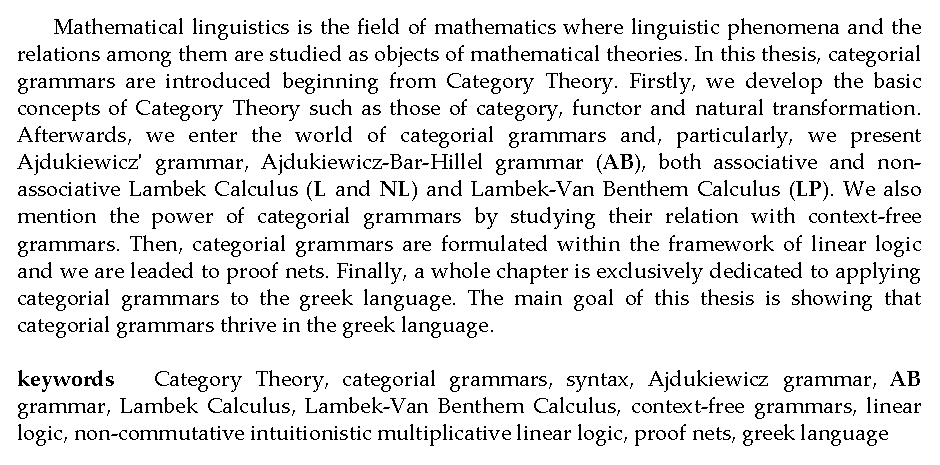
\includegraphics[scale=1]{abstract}
\end{center}
\chapter*{Πρόλογος}
\addcontentsline{toc}{chapter}{Πρόλογος}
Η παρούσα διπλωματική εργασία φιλοδοξεί να αναγνωσθεί ως μία μικρή εισαγωγή στη μαθηματική γλωσσολογία. Η μαθηματική γλωσσολογία υπάγεται στην υπολογιστική γλωσσολογία, η οποία εντάσσεται στην εφαρμοσμένη γλωσσολογία. Η \textbf{υπολογιστική γλωσσολογία}\index{γλωσσολογία!υπολογιστική} μπορεί να θεωρηθεί ως συνώνυμο της αυτόματης επεξεργασίας φυσικών γλωσσών,\footnote{Είθισται η χρήση του όρου \textit{φυσική γλώσσα} στην Επιστήμη των Υπολογιστών, όταν αναφερόμαστε σε κάποια από τις ομιλούμενες γλώσσες, καθώς υπάρχει ανάγκη διάκρισής του από τον όρο \textit{προγραμματιστική γλώσσα}.} αφού κύριος σκοπός της είναι η κατασκευή υπολογιστικών προγραμμάτων για την επεξεργασία λέξεων και κειμένων φυσικών γλωσσών.

Η \textbf{μαθηματική γλωσσολογία}\index{γλωσσολογία!μαθηματική} συγκαταλέγεται στην υπολογιστική, αλλά διαφοροποιείται σημαντικά από αυτήν. Αποτελεί την τομή της γλωσσολογίας και των μαθηματικών, δηλαδή είναι το πεδίο των μαθηματικών όπου εξετάζονται γλωσσικά φαινόμενα και οι σχέσεις μεταξύ τους ως αντικείμενα των μαθηματικών θεωριών \citep{bolshakov2004computational}. Επομένως, η μαθηματική γλωσσολογία αφορά κατά μείζονα λόγο τα εφαρμοσμένα μαθηματικά και δευτερευόντως τη γλωσσολογία. Στο σχήμα \ref{panorama}, αποτυπώνεται ένα πανόραμα της γλωσσολογίας προς διασάφηση των προηγουμένων.

\begin{figure}[ht]
\begin{center}
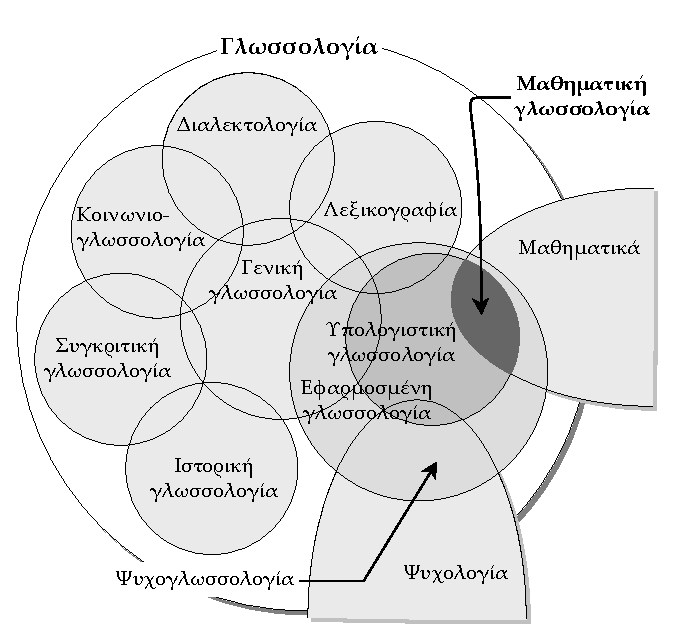
\includegraphics[scale=1]{glossologia.eps}
\caption{Η θέση της μαθηματικής γλωσσολογίας στο πανόραμα της γλωσσολογίας}
\label{panorama}
\end{center}
\end{figure}

Στη μαθηματική γλωσσολογία, όπως σε όλο το φάσμα των εφαρμοσμένων μαθηματικών, το πρόβλημα της μαθηματικής διατύπωσης και συστηματοποίησης θεωριών, οι οποίες έχουν διατυπωθεί είτε ανεπίσημα είτε ημιεπίσημα, ανακύπτει αρκετά συχνά. Ένα από τα πρώτα παραδείγματα είναι η μελέτη της δομής των προτάσεων, όπου ο Τσόμσκι \citep{citeulike:158531} επιχείρησε να αντικαταστήσει το ανεπίσημο σύστημα της ανάλυσης σε άμεσα συστατικά με τις ασυμφραστικές γραμματικές. Η ποιότητα της μαθηματικής διατύπωσης εξαρτάται τόσο από την πιστότητα στις αρχικές ιδέες όσο και από τη μαθηματική κομψότητα του συστήματος που δημιουργείται. Εδώ, επιχειρείται η συντακτική ανάλυση προτάσεων φυσικών γλωσσών από μαθηματική σκοπιά.

Στην εργασία αυτή, σημείο εκκίνησης είναι η \textbf{Θεωρία Κατηγοριών}, η οποία προσφέρει αυτά τα μαθηματικά αντικείμενα που αποζητούμε, έτσι ώστε να περιγράψουμε τα γλωσσικά φαινόμενα. Στο πρώτο κεφάλαιο, παρουσιάζονται οι βασικές έννοιες της Θεωρίας Κατηγοριών, όπως αυτές της κατηγορίας, του συναρτητή και του φυσικού μετασχηματισμού, και διάφορες καθολικές κατασκευές. Αν και οι έννοιες γύρω από τις οποίες περιστρέφονται τα άλλα τρία κεφάλαια αφορούν κατά βάση την κατηγορία και το συναρτητή, παρουσιάζουμε μια γενική εικόνα\footnote{Και πάλι, δεδομένης της βιβλιογραφίας, αρκετά περιορισμένη.} της Θεωρίας Κατηγοριών με στόχο τη συμπαγή θεμελίωση των επομένων.

Στο δεύτερο κεφάλαιο, έχοντας αναπτύξει τη Θεωρία Κατηγοριών, προχωρούμε στις \textbf{κατηγοριακές γραμματικές}. Από τη γένεσή τους, τουλάχιστον εννοιολογικά, χρησιμοποιούνταν οι όροι κατηγορία και συναρτητής για την περιγραφή τους. Ο Λάμπεκ κατάφερε να γεφυρώσει το μαθηματικό χάσμα εισάγοντας παράλληλα και έναν αυστηρό φορμαλισμό της μαθηματικής λογικής. Εδώ, παρουσιάζουμε τις κύριες κατηγοριακές γραμματικές: τις κλασικές γραμματικές, τους Λογισμούς Λάμπεκ και τους Λογισμούς Λάμπεκ-Φαν Μπένθεμ και δείχνουμε αυτήν τη μετάβαση. Πρέπει να σημειωθεί ότι ο Φαν Μπένθεμ είναι αυτός που εμφυσά δυναμικά τη σημασιολογία στις κατηγοριακές γραμματικές.

Στο τρίτο κεφάλαιο, επιχειρείται η κατάδειξη του ρόλου της \textbf{γραμμικής λογικής} στις κατηγοριακές γραμματικές. Μολονότι μετά την περιγραφή του βασικού πλέγματος των κατηγοριακών γραμματικών οι δρόμοι που μπορούμε να ακολουθήσουμε είναι πάρα πολλοί, επιλέξαμε αυτόν, επειδή μας προσφέρει τα \textbf{δίκτυα αποδείξεων}. Τα δίκτυα αποδείξεων αναπαριστούν την αποδεικτική διαδικασία μοναδικά, αφού συμπεριλαμβάνουν όλες τις δυνατές αποδείξεις μιας πρότασης σε ένα γράφημα. Επομένως, η συντακτική ανάλυση γίνεται επιτυχέστερα, γρηγορότερα και είναι μοναδική.

Στο τέταρτο κεφάλαιο, πραγματοποιείται μία απόπειρα εφαρμογής των κατηγοριακών γραμματικών και, ειδικότερα, της κατηγοριακής λογικής στην \textbf{ελληνική γλώσσα}. Σκοπός του κεφαλαίου αυτού είναι η κατάδειξη της ευδοκίμησης των προηγουμένων στη γλώσσα αυτή, κάτι το οποίο δεν υπάρχει στη βιβλιογραφία. Τα δίκτυα απόδειξης αποτελούν σημαντικό αρωγό στο έργο αυτό.

Καθ'όλη την εργασία, υπήρχε η ανησυχία αν όλος αυτός ο μαθηματικός φορμαλισμός έχει να προσφέρει στη μελέτη των φυσικών γλωσσών, αφού αυτό είναι το ζητούμενο. Επίσης, ισόβαρη ήταν και η ανησυχία κατά πόσο όλα αυτά μπορούν να αξιοποιηθούν υπολογιστικά, έτσι ώστε να μας δώσουν ορθούς τρόπους συντακτικής ανάλυσης χωρίς τη συνεχή μεσολάβηση του ανθρώπου. Ακόμα κι αν οι τελικές απαντήσεις σε αυτά τα ερωτήματα κρίνονται αβέβαιες, αξίζει να ρωτήσουμε, όχι μόνο λόγω, αλλά και έργω, διότι, αλλιώς, πώς θα μάθουμε;
\chapter*{Ευχαριστίες}
\addcontentsline{toc}{chapter}{Ευχαριστίες}
Η προκείμενη εργασία δε θα μπορούσε να πραγματοποιηθεί χωρίς την καθοδήγηση του επιβλέποντα κυρίου Πέτρου Στεφανέα, Λέκτορα ΕΜΠ, τον οποίο θα ήθελα να ευχαριστήσω θερμά, καθώς ήταν αυτός που με εισήγαγε στο θαυμαστό κόσμο της Θεωρίας Κατηγοριών και των κατηγοριακών γραμματικών. Επίσης, οφείλω να ευχαριστήσω τον Αναπληρωτή Καθηγητή κύριο Γεώργιο Κολέτσο και τον κύριο Αριστείδη Αραγεώργη, Λέκτορα ΕΜΠ, οι οποίοι δέχτηκαν να αξιολογήσουν το εν λόγω πόνημα και έλαβαν μέρος στην τριμελή επιτροπή.

Η εργασία αυτή αποτελεί το επιστέγασμα των σπουδών μου στη ΣΕΜΦΕ γι'αυτό και θα ήθελα να ευχαριστήσω δύο ανθρώπους που με βοήθησαν σε κρίσιμες φάσεις αυτής της πολυετούς προσπάθειας: την Τόνια για την αισιοδοξία της και για το κουράγιο που μου έδωσε σε πάρα πολλές δύσκολες στιγμές και το Μανιά για την ειλικρινή φιλία του και για το ότι έκανε τα μαθήματα να μοιάζουν πιο εύκολα.

Τέλος, θα ήθελα να ευχαριστήσω όλους εκείνους που με βοήθησαν να φτάσω εδώ, συμφοιτητές και μη, καθώς και τους γονείς μου, οι οποίοι με θυσίες μού έδωσαν τη δυνατότητα να σπουδάσω αυτό το αντικείμενο.
\cleardoublepage
\begingroup
\hypersetup{linkcolor=black}
\pdfbookmark[chapter]{Περιεχόμενα}{toc}
\tableofcontents

\clearpage

\pdfbookmark[chapter]{Κατάλογος σχημάτων}{lof}
\listoffigures
\cleardoublepage
\pdfbookmark[chapter]{Κατάλογος πινάκων}{anchor}
\listoftables

\endgroup

\bookmarksetupnext{bold}
\chapter{Στοιχεία Θεωρίας Κατηγοριών}
\pagenumbering{arabic}
Η \textbf{Θεωρία Κατηγοριών} είναι μια καθολική μαθηματική γλώσσα, όπως η Συνολοθεωρία. Η ειδοποιός διαφορά μεταξύ των δύο είναι ότι ενώ η Θεωρία Συνόλων περιστρέφεται γύρω από την έννοια του συνόλου, η κεντρική έννοια της Θεωρίας Κατηγοριών είναι η συνάρτηση. Να σημειωθεί πως η λέξη συνάρτηση χρησιμοποιείται προσεγγιστικά και όχι με την αυστηρή έννοια που έχει στη Συνολοθεωρία, δηλαδή μια απεικόνιση μεταξύ συνόλων.

Η έννοια της συνάρτησης είναι μία από τις θεμελιωδέστερες έννοιες στα μαθηματικά και στην επιστήμη. Ως μια πρώτη προσέγγιση, θα μπορούσε κανείς να πει πως η Θεωρία Κατηγοριών είναι η άλγεβρα των συναρτήσεων. Με τον ίδιο τρόπο που η θεωρία ομάδων αποτελεί μια αφαίρεση της ιδέας ενός συστήματος μεταθέσεων ενός συνόλου ή συμμετριών ενός γεωμετρικού αντικειμένου, έτσι και η θεωρία κατηγοριών ανακύπτει από την ιδέα ενός συστήματος συναρτήσεων μεταξύ αντικειμένων.

Οι κατηγορίες προέκυψαν, αρχικά, στα μαθηματικά από την ανάγκη ενός φορμαλισμού ικανού να περιγράψει τη μετάβαση από μία μαθηματική δομή ενός τύπου σε μία άλλη κάποιου άλλου. Οπότε, μια κατηγορία αντιπροσωπεύει ένα είδος μαθηματικών και μπορεί να θεωρηθεί ως ένα πεδίο μαθηματικής μελέτης. Η κατηγορία είναι επίσης μια μαθηματική δομή αυτή καθ'εαυτήν. Τέλος, η κατηγορία μπορεί να ιδωθεί ως μια κατασκευή που τυποποιεί τη μαθηματική περιγραφή μιας δομής. Αυτός είναι ο ρόλος της κατηγορίας ως θεωρίας.

Η Θεωρία Κατηγοριών ξεκινά με την παρατήρηση πως πολλές ιδιότητες μαθηματικών συστημάτων μπορούν να ενοποιηθούν και να απλοποιηθούν παρουσιαζόμενες με τη βοήθεια διαγραμμάτων βελών.

\begin{note}
Η βιβλιογραφία στη Θεωρία Κατηγοριών είναι πραγματικά πολύ μεγάλη. Σε αυτήν την εργασία, συμβουλευτήκαμε κυρίως το κλασικό \cite{lane1998categories}, καθώς και τα  \citep{PIERCE91}\citep{awodey2006category}\citep{van1995basic}.
\end{note}
\section{Τι είναι η κατηγορία}
\begin{definition}\label{category}\index{κατηγορία}
Μια \textbf{κατηγορία} $\mathcal{C}$ αποτελείται από:
\begin{itemize}
\item \textbf{Αντικείμενα} $ A,B,C,..., X,Y,... $
\item \textbf{Βέλη}\index{βέλος|see{μορφισμός}} ή \textbf{μορφισμούς}\index{μορφισμός} $ f,g,h,..., \alpha, \beta, \gamma,... $
\end{itemize}
Η συλλογή των αντικειμένων συμβολίζεται ως obj $\mathcal{C}$, ενώ αυτή των βελών ως arr $\mathcal{C}$.
\end{definition}
Επιπλέον, κάθε μορφισμός διαθέτει μία \textbf{αρχή}\index{μορφισμός!αρχή ή πεδίο ορισμού του} (πεδίο ορισμού) και ένα \textbf{τέλος}\index{μορφισμός!τέλος ή συμπεδίο ορισμού του} (συμπεδίο ορισμού)\index{συμπεδίο ορισμού} εντός της obj $\mathcal{C}$. Όταν η αρχή της $f$ είναι το $A$, δηλαδή $dom(f)=A$, και το τέλος της το $B$, δηλαδή $cod(f)=B$, γράφουμε $f:A \to B$. Μπορούμε επίσης να γράψουμε \begin{equation*}
A \xrightarrow{f} B.
\end{equation*}
Η συλλογή όλων των βελών με πεδίο ορισμού το Α και συμπεδίο ορισμού το Β συμβολίζεται ως $\mathcal{C}(A,B)$ ή ως $hom_{\mathcal{C}}(A,B)$.

Για κάθε ζεύγος μορφισμών
\begin{center}$A \xrightarrow{f} B$ και $ B \xrightarrow{g} C $\end{center}
υπάρχει μία καθορισμένη \textbf{σύνθεση μορφισμών}\index{σύνθεση μορφισμών}
\begin{center}$g \circ f: A \to C$\end{center}
\begin{displaymath}
	\xymatrix{
	A \ar@/_/[rr]_{g\circ f} \ar[r]^f & B \ar[r]^g & C
	}
\end{displaymath}
Κάθε αντικείμενο A έχει έναν \textbf{ταυτοτικό μορφισμό}\index{μορφισμός!ταυτοτικός} $1_{A}:A\to A$.

Τα παραπάνω προϋποτίθενται για την ικανοποίηση των ακόλουθων νόμων:
\begin{itemize}
\item Ταυτότητες: Αν $ A \xrightarrow{f} B $ τότε
\begin{center}$1_{B} \circ f=f $ και $ f \circ 1_{A}=f $\end{center}
\item Προσεταιριστικότητα: Αν $A \xrightarrow{f} B \xrightarrow{g} C \xrightarrow{h} D$ τότε
\begin{center}$ h \circ (g \circ f)=(h \circ g) \circ f : A \to D$.\end{center}\end{itemize}
Σχηματοποιώντας την παραπάνω σχέση, λαμβάνουμε
\begin{displaymath}
    \xymatrix{
A \ar@/_2pc/[rrr]_{h \circ (g \circ f)=(h \circ g) \circ f} \ar@/_/[rr]_{g\circ f} \ar[r]^f & B \ar@/^1.2pc/[rr]^{h\circ g} \ar[r]^g & C\ar[r]^h & D    
    }
\end{displaymath}
\begin{remark} Οφείλουμε να έχουμε πάντα υπόψη ότι η έννοια της άλγεβρας συναρτήσεων εισάγεται για δική μας διευκόλυνση και δεν αποτελεί επίσημο ορισμό της κατηγορίας. Η έννοια της κατηγορίας ορίζεται, όπως είδαμε, \textbf{αξιωματικά}. Τα αντικείμενα της κατηγορίας δεν είναι απαραιτήτως σύνολα και οι μορφισμοί δεν είναι απαραιτήτως συναρτήσεις, όπως τις ξέρουμε. Ως συνήθως, οι αξιωματικοί ορισμοί μάς προσφέρουν μεγάλη ευελιξία στην κατασκευή των κατηγοριών. Αυτή η ευελιξία είναι κρίσιμη στην εφαρμογή των τελευταίων.
\end{remark}
Ένα σημαντικό εργαλείο για την εξοικείωση με τη Θεωρία Κατηγοριών είναι τα διαγράμματα. Τα διαγράμματα αξιοποιούνται στην κατάδειξη και απόδειξη ιδιοτήτων των κατηγορικών κατασκευών.
\begin{definition}\label{diagram}
Ένα \textbf{διάγραμμα}\index{διάγραμμα!κατηγορίας} μιας κατηγορίας $\mathcal{C}$ είναι μια συλλογή κορυφών και ακμών, στις οποίες αντιστοιχούν \textbf{με συνέπεια} αντικείμενα και βέλη της $\mathcal{C}$. Η συνέπεια έγκειται στο ότι εάν σε μία ακμή έχει αποδοθεί το βέλος $f$, με πεδίο ορισμού το A και συμπεδίο το Β, τότε, υποχρεωτικά, οι κορυφές τις οποίες το βέλος ενώνει πρέπει να έχουν ονομαστεί Α και Β.
\end{definition} 
\begin{definition}\label{commutativeDiagram}
Ένα διάγραμμα μιας κατηγορίας $\mathcal{C}$ είναι \textbf{αντιμεταθετικό}\index{διάγραμμα!αντιμεταθετικό} αν για κάθε ζεύγος κορυφών K και L, όλα τα μονοπάτια του διαγράμματος από το K στο L είναι ίσα, δηλαδή αν κάθε μονοπάτι του διαγράμματος ορίζει ένα βέλος και αυτά τα βέλη είναι ίσα στην $\mathcal{C}$. Συνεπώς, η έκφραση «το διάγραμμα
\begin{displaymath}
\xymatrix
{
K \ar[d]_{g'} \ar[r]^{f'} & N \ar[d]^g \\
M \ar[r]_f & L
}
\end{displaymath}
είναι αντιμεταθετικό»
και η έκφραση $f\circ g'=g\circ f'$ θεωρούνται ισοδύναμες.
\end{definition} 
Στο νόμο της προσεταιριστικότητας, όπως τον δείξαμε προηγουμένως, το διάγραμμα είναι αντιμεταθετικό και τα αντίστοιχα βέλη είναι ίσα μεταξύ τους.
\begin{note}
Ο ορισμός του διαγράμματος, όπως τον διατυπώσαμε, δεν είναι αυστηρός. Αρκούμαστε, όμως, στην εξήγηση της αντιμεταθετικότητας ενός διαγράμματος, η οποία εν πολλοίς παίζει τον ρόλο των εξισώσεων στη Θεωρία Κατηγοριών.
\end{note}
\paragraph{Mερικά στοιχειώδη παραδείγματα κατηγοριών}
\label{ElementaryCategories}
\begin{itemize}
\item Η κατηγορία \textbf{0} είναι η κενή κατηγορία. Δεν έχει ούτε αντικείμενα, ούτε βέλη.
\item Η κατηγορία \textbf{1} είναι η κατηγορία $ \circlearrowleft $ με ένα αντικείμενο και ένα βέλος.
\item Η κατηγορία \textbf{2} είναι η κατηγορία $ \circlearrowleft \to \circlearrowleft $ με δύο αντικείμενα $A,B$ και μόνο ένα βέλος, $A \to B$, όχι της ταυτότητας.
\item Η κατηγορία \textbf{3} είναι η κατηγορία με τρία αντικείμενα και δύο βέλη, διαφορετικά από αυτά των ταυτοτήτων.
\begin{displaymath}
\xymatrix{
&\circlearrowleft \ar[dl]  \\
\circlearrowleft \ar[rr] && \circlearrowleft \ar[ul]
}
\end{displaymath}
\end{itemize}
\paragraph{Συνήθη παραδείγματα κατηγοριών}
\label{ExamplesOfCategories}
\begin{enumerate}
\item Η κατηγορία \textbf{Set}. Τα σύνολα είναι τα αντικείμενά της και οι συναρτήσεις μεταξύ αυτών τα βέλη της. Η ταυτοτική συνάρτηση αντιστοιχεί στον ταυτοτικό μορφισμό και η σύνθεση συναρτήσεων στη σύνθεση μορφισμών.
\item Η κατηγορία \textbf{Grp}. Αντικείμενά της είναι οι ομάδες και βέλη της οι μορφισμοί μεταξύ των ομάδων αυτών. Ομοίως με τη \textbf{Set}, ο ταυτοτικός μορφισμός μιας ομάδας αντιστοιχεί στον ταυτοτικό μορφισμό ενός αντικειμένου, ενώ η σύνθεση μορφισμών μεταξύ ομάδων στη σύνθεση βελών.
\item Η κατηγορία \textbf{Rel}. Έχει τα ίδια αντικείμενα με τη \textbf{Set}, αλλά εδώ κάθε βέλος $R: A\to B$ είναι μία διμελής σχέση $R\subseteq A \times B$. Δοθέντων δύο βελών $R: A\to B$ και $S: B\to C$, η σύνθεσή τους αποτελεί το \textbf{σχεσιακό γινόμενο}
\begin{center}
$R\circ S :A\to C = \{(a,c)\in A \times C \mid \exists b \in B$ ώστε $(a,b)\in R$ και $(b,c)\in S\}$.
\end{center}
Τα ταυτοτικά βέλη $id_{A}:A\to A$ δίνονται από τις διαγώνιες σχέσεις $\{(a,a)\mid a\in A\}$.
\item Η κατηγορία \textbf{Mon}. Αποτελείται από μόνο ένα αντικειμένο, το μονοειδές. Τα βέλη της κατηγορίας αυτής είναι τα στοιχεία του μονοειδούς, το ταυτοτικό βέλος είναι το μοναδιαίο στοιχείο $u$, ενώ η σύνθεση βελών είναι η διμελής πράξη $m \cdot n$ του μονοειδούς.

Ένα \textbf{μονοειδές}\index{μονοειδές}, γνωστό και ως ημιομάδα με μοναδιαίο στοιχείο, είναι ένα σύνολο M εφοδιασμένο με μια διμελή πράξη $\cdot : M \times M \to M$ και ένα μοναδικό στοιχείο $u \in M$ τέτοιο ώστε $\forall x,y,z \in M$
\begin{center}
$x\cdot (y \cdot z)=(x\cdot y)\cdot z$
και $u \cdot x = x \cdot u = x$
\end{center}
\item Η κατηγορία του \textbf{ομαδοειδούς}\index{ομαδοειδές}. Αποτελείται από μια συλλογή αντικειμένων και βασική ιδιότητά του είναι πως κάθε βέλος του είναι ισομορφισμός, δηλαδή αντιστρέψιμο, όπως θα δούμε παρακάτω.
\item Η κατηγορία \textbf{Poset}, των μερικώς διατεταγμένων συνόλων\footnote{Η λέξη Poset προέρχεται από τη συνένωση των λέξεων \textbf{P}artially \textbf{o}rdered set.} και των μονότονων συναρτήσεων μεταξύ τους.

Μία \textbf{μερική διάταξη}\index{μερική διάταξη} είναι μια διμελής σχέση σε ένα σύνολο $X$, η οποία είναι
\begin{enumerate} [i.]
\item  \textbf{αυτοπαθής} ($x\leq x$, $\forall x \in X$)
\item \textbf{αντισυμμετρική} (αν $x\leq y$ και $y \leq x$, τότε $x=y$, $\forall x,y \in X$)
\item \textbf{μεταβατική} (αν $x\leq y$ και $y\leq z$, τότε $x\leq z$, $\forall x,y,z \in X$).
\end{enumerate}
Έστω το ζεύγος $\langle P, \sqsubseteq \rangle$, όπου $P$ σύνολο και $(\sqsubseteq)\subseteq P \times P$ μια μερική διάταξη. Τότε μια \textbf{μονότονη} συνάρτηση $f$ από το $\langle P, \sqsubseteq \rangle$ στο $\langle Q, \leqslant \rangle$ είναι μια συνάρτηση $f\in Q^P$ τέτοια ώστε αν $a \sqsubseteq b$, τότε $f(a)\leqslant f(b)$, $\forall a,b\in P$.
\item Η κατηγορία $\Omega$-\textbf{Alg}. Αντικείμενά της είναι οι Ω-άλγεβρες και βέλη της οι μορφισμοί μεταξύ τους.

Έστω $\Omega$ ένα σύνολο τελεστικών συμβόλων, εφοδιασμένο με μια απεικόνιση $a \in \mathbb{N}^{\Omega}$, τέτοια ώστε για κάθε $\omega \in \Omega$, η $a(\omega)$ να είναι η \textbf{τάξη}\footnote{Αποδίδουμε με τον όρο τάξη την αγγλική λέξη \textit{arity}.} του $\omega$. Το $\Omega_{n}=\{s \in \Omega : a(s)=n\}$ καλείται σύνολο των ν-τάξιων τελεστικών συμβόλων του $\Omega$. Μία \textbf{Ω-άλγεβρα} είναι ένα ζεύγος $\langle A,\delta \rangle$, όπου Α είναι ένα σύνολο που καλείται φορέας της άλγεβρας και $\delta$ μια οικογένεια πράξεων στο Α, τέτοια ώστε \begin{center} $\delta=\bigcup_{s \in \Omega}(\delta_{s})$ και $\delta_{s} \in A^{A^{(n)}}$ για κάθε $s \in \Omega_{n}$ και για κάθε $n \in \mathbb{N}$. \end{center}
Για κάθε $s \in \Omega$, το $\delta_{s}$ καλείται \textbf{ερμηνεία}\index{ερμηνεία} του s.

Ένας μορφισμός μεταξύ μιας Ω-άλγεβρας $\langle A,\delta \rangle$ και μιας άλλης $\langle B,\varepsilon \rangle$ είναι μια απεικόνιση $f \in B^{A}$ ώστε
\begin{center}
$f(\delta_{s}(a_{1},...,a_{n}))=\varepsilon_{s}(f(a_{1}),...,f(a_{n})) $ για κάθε $ \langle a_{1},...,a_{n} \rangle \in A^{(n)}, s \in \Omega_{n}, n \in \mathbb{N}$.
\end{center}
\end{enumerate}
Ας δούμε τώρα, μια εξαιρετικά χρήσιμη θεώρηση μιας κατηγορίας, η οποία άπτεται της μαθηματικής λογικής. Πρόκειται για την κατηγοριακή λογική\index{λογική!κατηγοριακή} κατά Λάμπεκ, της οποίας την περιγραφή λαμβάνουμε από το Στεφανέα \citep{stefaneas}. Οι λογικές παραγωγές της είναι της μορφής
\begin{equation*}A_{1}A_{2}...A_{n}\to A_{n+1}
\end{equation*}
όπου οι φόρμουλες $A_{1},...,A_{n}$ είναι οι υποθέσεις που παράγουν λογικά το $A_{n+1}$. Αρχικά, ορίζουμε το πολυγράφημα.
\begin{definition}
Ένα \textbf{πολυγράφημα}\index{πολυγράφημα} αποτελείται από
\begin{itemize}
\item μία κλάση βελών $A$ καλούμενα \textbf{λογικές παραγωγές}\index{παραγωγή!λογική}
\item μία κλάση αντικειμένων $O$ καλούμενα \textbf{φόρμουλες}
\end{itemize}
και δύο απεικονίσεις
\begin{enumerate}[(i)]
\item $\theta_{0}:A\to O^{*}$ (αρχή)
\item $\theta_{1}:A\to O$ (τέλος).
\end{enumerate}
Το $O^{*}$ αποτελείται από λίστες της μορφής $A_{i_{1}}A_{i_{2}}...A_{i_{k}}$, όπου $A_{i_{1}},A_{i_{2}},...,A_{i_{k}}\in O$. Οπότε, για κάθε βέλος του πολυγραφήματος
\begin{equation*}
f:A_{1}A_{2}...A_{n}\to A_{n+1}
\end{equation*}
έχουμε ότι
\begin{center}
$\theta_{0}(f)=A_{1}A_{2}...A_{n}$ και $\theta_{1}(f)=A_{n+1}$
\end{center}
\end{definition}
Τώρα, μπορούμε να ορίσουμε το σύστημα λογικής παραγωγής κατά Λάμπεκ.
\begin{definition}
Ένα \textbf{σύστημα λογικής παραγωγής κατά Λάμπεκ} είναι ένα πολυγράφημα, το οποίο ικανοποιεί τα εξής:
\begin{itemize}
\item Για κάθε αντικείμενο $A$ υπάρχει ένας ταυτοτικός μορφισμός $1_{A}:A\to A$.
\item Για κάθε δύο μορφισμούς $f:\Theta\to A$ και $g:\Gamma A \Delta\to B$ υπάρχει ένας μορφισμός $g\langle f\rangle :\Gamma\Theta\Delta\to B$ τέτοιος ώστε
\begin{prooftree}
\AxiomC{$f:\Theta\to A$}
\AxiomC{$g:\Gamma A\Delta\to B$}
\BinaryInfC{$g\langle f\rangle :\Gamma\Theta\Delta\to B$}
\end{prooftree}
δηλαδή ισχύει η τομή κατά Γκέντζεν.\footnote{Στο επόμενο κεφάλαιο, θα επεκταθούμε σχετικά με το συγκεκριμένο λογικό κανόνα.}
\end{itemize}
\end{definition}
\begin{definition}\label{subcategory}
Έστω μια κατηγορία $\mathcal{C}$. Η κατηγορία $\mathcal{B}$ καλείται \textbf{υποκατηγορία}\index{κατηγορία!υποκατηγορία} της $\mathcal{C}$ αν ισχύουν τα ακόλουθα
\begin{enumerate}[(i)]
\item Κάθε αντικείμενο της $\mathcal{B}$ ανήκει στη $\mathcal{C}$.
\item Για κάθε αντικείμενο B και B' της $\mathcal{B}$ $hom_{\mathcal{B}}(B,B') \subset hom_{\mathcal{C}}(B,B')$.
\item Οι συνθέσεις και τα ταυτοτικά βέλη είναι ίδια στην $\mathcal{B}$ και στη $\mathcal{C}$.
\end{enumerate}
\end{definition}
\begin{definition}\label{dual}
Για κάθε κατηγορία $\mathcal{C}$, υπάρχει η \textbf{δυϊκή}\index{κατηγορία!δυϊκή} αυτής και συμβολίζεται ως $C^{op}$. Τα αντικείμενα της τελευταίας είναι τα ίδια με της πρώτης, ενώ τα βέλη της $C^{op}$ είναι τα αντίθετα αυτών της $\mathcal{C}$. Δηλαδή, εάν το $f:A\to B$ είναι ένα βέλος της $\mathcal{C}$, τότε το $g:B\to A$ είναι ένα βέλος της $C^{op}$.
\end{definition}
\begin{proposition}\label{DualCategory}
Η δυϊκή μιας κατηγορίας είναι και αυτή κατηγορία.
\end{proposition}
\begin{proof}
Από τον ορισμό, προκύπτει άμεσα.
\end{proof}
\begin{proposition}\label{dualOfdual}
Για κάθε κατηγορία $\mathcal{C}$ ισχύει $(\mathcal{C}^{op})^{op}=\mathcal{C}$.
\end{proposition}
\begin{proof}
Πάλι από τον ορισμό, τα αντικείμενα της $(\mathcal{C}^{op})^{op}$ είναι ίδια με αυτά της $\mathcal{C}$, ενώ τα αντεστραμμένα βέλη των αντεστραμμένων βελών της $\mathcal{C}^{op}$, δηλαδή τα βέλη της $(\mathcal{C}^{op})^{op}$, έχουν την ίδια φορά με αυτά της $\mathcal{C}$.
\end{proof}
\begin{remark}[Αρχή δυϊκότητας]\label{dualityPrinciple}\index{αρχή δυϊκότητας}
Κάθε κατηγορική έννοια έχει και τη δυϊκή της. Έτσι, όπως έχουμε πεδίο ορισμού και συμπεδίο ορισμού, προκύπτουν τα αρχικά και τελικά αντικείμενα, οι εξισωτές και οι συνεξισωτές, τα γινόμενα και τα συγγινόμενα, τα όρια και τα συνόρια, έννοιες τις οποίες θα δούμε αναλυτικά παρακάτω. Κάθε πρόταση που αφορά μια έννοια στην $\mathcal{C}$, η ίδια ισχύει και για την αντίστοιχη δυϊκή πρόταση της $C^{op}$. Συνεπώς, όποτε ορίζουμε κάποια έννοια, τις περισσότερες φορές θα ακολουθεί και η δυϊκή αυτής. Επίσης, αν $\Sigma$ είναι μια πρόταση της $\mathcal{C}$ και $\Sigma^*$ μια πρόταση της $C^{op}$, τότε $\Sigma^{**}=\Sigma$ και, αν μια πρόταση εμπεριέχει ένα διάγραμμα, τότε η δυϊκή αυτής εμπεριέχει το ίδιο διάγραμμα με τα βέλη αντεστραμμένα. Τα παραπάνω μπορούν να συνοψισθούν στο ακόλουθο:
\begin{center}
\AxiomC{$f:A \to B$ στη $\mathcal{C}$} 
			  \UnaryInfC{$g:B\to A$ στη $\mathcal{C}^{op}$}
			  \DisplayProof
\end{center}
\end{remark}
Είδαμε, λοιπόν, τι είναι η κατηγορία και μερικά παραδείγματα κατηγοριών, διάφορες άλλες βασικές έννοιες, καθώς και την πολύ σημαντική για την παρούσα εργασία άποψη ότι μια τυχαία κατηγορία μπορεί να αντιμετωπιστεί ως ένα τυπικό σύστημα συμπερασμού. Ας προχωρήσουμε τώρα στον ορισμό της δεύτερης σημαντικότερης έννοιας της Θεωρίας Κατηγοριών: την έννοια του συναρτητή.
\section{Τι είναι ο συναρτητής}
\label{whatAFunctorIs}
Ελαφρώς απομακρυνόμενοι από το τοπίο των κατηγοριών, παρατηρούμε ότι αυτές ξεκινούν να δημιουργούν μια δομή, η οποία διαφαίνεται από τις απεικονίσεις μεταξύ τους. Αυτές τις απεικονίσεις τις αποκαλούμε συναρτητές.
\begin{definition}\label{functor}
Ένας \textbf{συναρτητής}\index{συναρτητής}
\begin{center}
$F:\mathcal{C}\to \mathcal{D}$
\end{center}
μεταξύ δύο κατηγοριών $\mathcal{C}$ και $\mathcal{D}$ είναι μία απεικόνιση αντικειμένων σε αντικείμενα και βελών σε βέλη, έτσι ώστε
\begin{itemize}
\item $F(f:A \to B)=F(f): F(A) \to F(B)$
\item $F(g \circ f)=F(g) \circ F(f)$
\item $F(1_{A})=1_{F(A)}$
\end{itemize}
\end{definition}
Με τον ίδιο τρόπο που ορίσαμε τη σύνθεση βελών, αναλόγως ορίζουμε και τη σύνθεση συναρτητών.
\begin{definition}\label{compositionOfFunctors}
Έστω $F:\mathcal{C}\to\mathcal{D}$ και $G:\mathcal{D}\to\mathcal{E}$ συναρτητές. Τότε η \textbf{σύνθεση}\index{συναρτητής!σύνθεση} των δύο αυτών συναρτητών \begin{equation*}
(G\circ F):\mathcal{C}\to\mathcal{E}
\end{equation*}
είναι επίσης συναρτητής.
\end{definition}
\begin{definition}\label{unitaryFunctor}
Για κάθε κατηγορία $\mathcal{C}$, ο \textbf{ταυτοτικός συναρτητής}\index{συναρτητής!ταυτοτικός} $I_{\mathcal{C}}$ απεικονίζει κάθε αντικείμενο και κάθε βέλος της $\mathcal{C}$ στον εαυτό του.
\end{definition}
\begin{definition}\label{endofunctor}
Ένας συναρτητής $F:\mathcal{C}\to\mathcal{C}$ λέγεται \textbf{ενδοσυναρτητής}\index{συναρτητής!ενδοσυναρτητής} στη $\mathcal{C}$.
\end{definition}
Συνεπώς, η σύνθεση συναρτητών, δηλαδή η σύνθεση των βελών και, αντίστοιχα, η σύνθεση των αντικειμένων δύο κατηγοριών ευσταθεί και, ως εκ τούτου, λαμβάνουμε άλλη μια κατηγορία, γνωστή ως \textbf{Cat}. Τα αντικείμενα της κατηγορίας αυτής είναι κατηγορίες, ενώ τα βέλη της συναρτητές.
\begin{remark}\label{foundationalQuestions}
Με την ανάδυση της κατηγορίας \textbf{Cat} και φέρνοντας κατά νου το \textit{Παράδοξο του Ράσελ}\index{Ράσελ!παράδοξο του}\footnote{Έστω $S=\{x : x \notin x \}$. Τότε $S \in S$ αν και μόνο αν $S \notin S$.} μπορούμε να παρατηρήσουμε πως ο ορισμός της είναι προβληματικός. Στη Θεωρία Κατηγοριών αυτό το πρόβλημα ξεπερνιέται με τη διάκριση των κατηγοριών σε \textbf{μικρές}\index{κατηγορία!μικρή} και \textbf{μεγάλες}\index{κατηγορία!μεγάλη}, όπου μικρές είναι οι κατηγορίες των οποίων τα αντικείμενα μπορούν να θεωρηθούν και σύνολα. Επομένως, η \textbf{Cat} ορίζεται πλέον καλώς ως η κατηγορία των μικρών κατηγοριών, η οποία είναι μία μεγάλη κατηγορία.
\end{remark}
Για την περαιτέρω κατανόηση και εξοικείωση με την έννοια του συναρτητή παρατίθενται μερικά παραδείγματα.
\paragraph{Παραδείγματα Συναρτητών}
\begin{enumerate}
\item \label{powersetFunctor}
Ο συναρτητής του δυναμοσυνόλου $P :\textbf{Set} \to \textbf{Set}$ είναι ένας ενδοσυναρτητής της \textbf{Set}. Η συνάρτηση αντικειμένων αντιστοιχίζει σε καθε σύνολο $X$ το σύνηθες δυναμοσύνολο $P(X)$ με στοιχεία όλα τα υποσύνολα $S\subset X$, ενώ η συνάρτηση βελών αντιστοιχίζει κάθε συνάρτηση $f:X \to Y$ στην  $P(f): P(X) \to P(Y)$, η οποία απεικονίζει κάθε $S \subset X$ στο σύνολο $f(S)$, όπου $f(S) \subset Y$. Ο συναρτητής είναι καλώς ορισμένος, επειδή ισχύει ότι $P(1_{x})=1_{P(X)}$ και $P(g \circ f)= P(g) \circ  P(f)$.
\item Ο \textbf{εγκλειστικός συναρτητής}\index{συναρτητής!εγκλειστικός} $Inc:\textbf{Vec}_{fd}\rightarrow\textbf{Vec}$, ο οποίος απεικονίζει κάθε διανυσματικό χώρο πεπερασμένης διάστασης στον εαυτό του, περιλαμβάνοντας όμως στην κατηγορία που καταλήγει και όλους τους υπόλοιπους, δηλαδή και τους απειροδιάστατους χώρους.
\item \label{constantFunctor}
Ο \textbf{σταθερός συναρτητής}\index{συναρτητής!σταθερός} απεικονίζει κάθε αντικείμενο $A$ της $\mathcal{C}$ σε ένα αντικείμενο $B$ της $\mathcal{D}$ και κάθε βέλος της $\mathcal{C}$ στο ταυτοτικό βέλος της $\mathcal{D}$.
\item \label{forgetfulFunctor}
Ο \textbf{επιλήσμων συναρτητής}\index{συναρτητής!επιλήσμων} $U: \bf Mon \to \bf Set$ απεικονίζει κάθε μονοειδές $(M,\cdot,e)$ στο σύνολο M και κάθε ομοιομορφισμό $h: (M,\cdot,e) \to (M',\cdot ',e')$ στην αντίστοιχη συνάρτηση $h:M \to M'$ μεταξύ των συγκεκριμένων συνόλων. Ονομάζεται έτσι διότι «ξεχνά» τη δομή που χαρακτηρίζει το μονοειδές.
\item \label{freeFunctor}
Ο \textbf{ελεύθερος συναρτητής}\index{συναρτητής!ελεύθερος}, σε αντίθεση με τον επιλήσμονα συναρτητή, δημιουργεί μια πλουσιότερη δομή σε μια κατηγορία. Παραδείγματος χάρη, ελεύθερος είναι ο συναρτητής $F: \textbf{Set}\to \textbf{Grp}$, ο οποίος αντιστοιχίζει κάθε σύνολο στην ελεύθερη ομάδα\footnote{Μία ομάδα $G$ ονομάζεται \textbf{ελεύθερη} αν υπάρχει σύνολο $S\subset G$ τέτοιο ώστε κάθε στοιχείο της $G$ να μπορεί να γραφτεί με έναν και μοναδικό τρόπο ως γινόμενο πεπερασμένου πλήθους στοιχείων του $S$ και των αντιστρόφων αυτών των στοιχείων.} που δημιουργείται από αυτό και κάθε συνάρτηση στον ομομορφισμό μεταξύ των αντίστοιχων ελεύθερων ομάδων.
\end{enumerate}
\begin{definition}
Έστω ο συναρτητής $F: \mathcal{C}\to \mathcal{D}$. Τότε ο συναρτητής $F^{op}: \mathcal{C}^{op}\to \mathcal{D}$ λέγεται \textbf{ανταλλοίωτος}\index{συναρτητής!ανταλλοίωτος ή αντίθετος} ή \textbf{αντίθετος} και απεικονίζει κάθε αντικείμενο $A$ της $\mathcal{C}$ σε ένα αντικείμενο $F^{op}(A)$ της $\mathcal{D}$ και κάθε βέλος $f:A\to B$ σε ένα βέλος $F^{op}(f):F^{op}(B)\to F^{op}(A)$ της $\mathcal{D}$.
\end{definition}
\begin{example}
Όπως ορίσαμε το συναρτητή του δυναμοσυνόλου, $P$, μπορούμε να ορίσουμε τον αντίθετό του, $P^{op}:\textbf{Set}^{op}\to \textbf{Set}$, για τον οποίο ισχύει ότι
\begin{center}
$A \mapsto P^{op}(A)=\{X\mid X \subseteq A\}$\\
$f:A\to B \mapsto P^{op}(f):P^{op}(B)\to P^{op}(A)$, όπου $P^{op}(f)(Y)=f^{-1}[Y]$.
\end{center}\end{example}

\begin{definition}\label{homsetFunctor}
Έστω μια κατηγορία $\mathcal{C}$. Αν $A$ αντικείμενό της, τότε ορίζεται ο συναρτητής $\mathcal{C}(A,-):\mathcal{C}\to \textbf{Set}$. Αυτός ο συναρτητής αντιστοιχίζει κάθε αντικείμενο $B$ της $\mathcal{C}$ στο σύνολο $\mathcal{C}(A,B)$ των βελών από το $A$ στο $B$ και κάθε βέλος $f:B\to C$ της $\mathcal{C}$ στη συνάρτηση $\mathcal{C}(A,f):\mathcal{C}(A,B)\to \mathcal{C}(A,C)$ με $\mathcal{C}(A,f)(g:A \to B)=f\circ g$, όπου προφανώς η σύνθεση στο δεξί μέλος της ισότητας διενεργείται εντός της $\mathcal{C}$. Ο συναρτητής $\mathcal{C}(A,-)$ λέγεται \textbf{συναρτητής ομομορφισμού}\index{συναρτητής!ομομορφισμού} (hom-functor). Αντίστοιχα ορίζεται και ο \textbf{ανταλλοίωτος συναρτητής ομομορφισμού}\index{συναρτητής!ανταλλοίωτος ομομορφισμού} $\mathcal{C}(-,B)$.
\end{definition}
Σε αυτήν την ενότητα, λοιπόν, είδαμε το συναρτητή, ο οποίος γενικεύει την έννοια της συνάρτησης, αφού τα ορίσματά του είναι και συναρτήσεις. Στην επόμενη ενότητα θα δούμε πώς σχετίζονται οι συναρτητές μεταξύ τους.
\section{Τι είναι ο φυσικός μετασχηματισμός}
Το πλέγμα των κατηγοριών και των συναρτητών μεταξύ των κατηγοριών εμπλουτίζεται ακόμα περισσότερο με την εμφάνιση απεικονίσεων μεταξύ των συναρτητών. Αυτές τις απεικονίσεις τις αποκαλούμε φυσικούς μετασχηματισμούς.
\begin{definition}\label{naturalTransformation}
Έστω δύο συναρτητές $F,G:\mathcal{C}\to \mathcal{D}$. Ένας \textbf{φυσικός μετασχηματισμός}\index{φυσικός μετασχηματισμός} $\vartheta : F\dot{\to}G$ είναι μια απεικόνιση, η οποία αντιστοιχίζει κάθε αντικείμενο A της $\mathcal{C}$ σε ένα βέλος $\vartheta_{A}:F(A)\to G(A)$ της $\mathcal{D}$, το οποίο καλείται \textbf{συνιστώσα}\index{φυσικός μετασχηματισμός!συνιστώσα του} του $\vartheta$ στη $\mathcal{C},$ έτσι ώστε για κάθε μορφισμό $f:A\to B$ να ισχύει \begin{center}
$\vartheta_{B}\circ F(f) = G(f) \circ \vartheta_{A}$
\end{center} δηλαδή το διάγραμμα
\begin{displaymath}
\xymatrix{
F(A) \ar[d]_{\vartheta_{A}} \ar[r]^{F(f)} & F(B) \ar[d]^{\vartheta_{B}}\\
G(A) \ar[r]_{G(f)} & G(B)
}
\end{displaymath}
να είναι αντιμεταθετικό. Όταν ισχύει η προηγούμενη σχέση, μπορούμε επίσης να πούμε πως ο μορφισμός $\vartheta_{A}:F(A)\to G(A)$ είναι \textbf{φυσικός}\index{μορφισμός!φυσικός} στο Α.
\end{definition}
\begin{definition}\label{naturalIsomorphism}
Αν κάθε συνιστώσα $\vartheta_{A}$ του $\vartheta$ είναι ισομορφισμός\footnote{Όπως προαναφέρθηκε, ισομορφισμός λέγεται κάθε αντιστρέψιμο βέλος. Στην επόμενη ενότητα θα ασχοληθούμε εκτενέστερα με την έννοια αυτή.} στην $\mathcal{D}$, τότε ο $\vartheta$ ονομάζεται \textbf{φυσικός ισομορφισμός}\index{φυσικός ισμορφισμός}. Δύο συναρτητές λέγονται \textbf{φυσικά ισομορφικοί} ή απλώς \textbf{ισομορφικοί}\index{συναρτητής!ισομορφικός}, αν υπάρχει φυσικός ισομορφισμός μεταξύ αυτών.
\end{definition}
\begin{remark}
Αν φανταστούμε το συναρτητή $F$ ως αυτόν που μας δίνει την εικόνα όλων των αντικειμένων και των βελών της $\mathcal{C}$ στην $\mathcal{D}$, τότε ο φυσικός μετασχηματισμός $\vartheta$ είναι μία συλλογή βελών που απεικονίζουν (ή μεταφράζουν) την εικόνα του $F$ στην εικόνα του $G$, έτσι ώστε το διάγραμμα
\begin{displaymath}
\xymatrix{
F(A) \ar[dd]_{F(h)} \ar[dr]^{F(f)} \ar[rrr]^{\vartheta_{A}} &&& G(A) \ar[dd]_<(.2){G(h)}|!{[d]}\hole \ar[dr]^{G(f)} \\
& F(B) \ar[dl]^{F(g)} \ar[rrr]^<(.2){\vartheta_{B}} &&& G(B) \ar[dl]^{G(g)} \\
F(C) \ar[rrr]_{\vartheta_{C}} &&& G(C)
}
\end{displaymath}
να είναι αντιμεταθετικό.
\end{remark}
Ακολουθεί ένα παράδειγμα έτσι ώστε να καταστεί αντιληπτό το τι νοούμε ως φυσικό και ειδικότερα ισομορφικό μετασχηματισμό.
\begin{proposition}\label{naturalIsomorpismExample}
Κάθε ομάδα είναι φυσικά ισόμορφη με την αντίθετή της.\footnote{Αν $G$ μια ομάδα, τότε η αντίθετή της $G^{op}$ αναφέρεται στο ίδιο σύνολο, ενώ οι μορφισμοί της είναι αντεστραμμένοι, δηλαδή $a \ast b \in G \mapsto b \ast^{op} a \in G^{op}$.} Αυτό μπορεί να οριστεί ως συναρτητής από ομάδες σε ομάδες, έτσι ώστε $f^{op}=f$ για κάθε ομομορφισμό ομάδων $f: G \to H$. Για τον ορισμό αυτού του συναρτητή, η απεικόνιση $f^{op}: G^{op} \to H^{op}$ πρέπει να είναι ομομορφισμός. Αυτό ισχύει πράγματι, καθώς παρατηρούμε πως για κάθε $a,b \in G$ και $f: G \to H$ έχουμε ότι
\begin{center}
$f^{op}(a\ast b)=f(b\ast a)=f^{op}(a) \ast^{op} f^{op}(b)$
\end{center}
Το τελευταίο μάς δείχνει τι χρειάζεται για να επιβεβαιώσουμε τη φυσικότητα του μετασχηματισμού: πρέπει να αποδείξουμε ότι ο ταυτοτικός συναρτητής μεταξύ ομάδων είναι φυσικά ισομορφικός με τον αντίθετο συναρτητή, όπως αυτός ορίστηκε πρωτύτερα. Έτσι, πρέπει να δώσουμε τον ισομορφισμό $\vartheta_{G}:G\to G^{op}$ ώστε το σχετικό διάγραμμα που θα ορίζει τη φυσικότητα να είναι αντιμεταθετικό.
\end{proposition}
\begin{proof}
Έστω $\vartheta_{G}(a)=a^{-1}, \forall a \in G$. Έχουμε ότι $(ab)^{-1}=b^{-1}a^{-1}$ και $(a^{-1})^{-1}=a$, δηλαδή η $\vartheta_{G}$ είναι η αντίστροφη του εαυτού της. Έστω, τώρα, $f: G \to H$ ένας ομομορφισμός ομάδων. Έχοντας υπόψη ότι $f^{op}=f$ και $f(a)^{-1}=f(a^{-1})$, το διάγραμμα
\begin{displaymath}
\xymatrix{
G \ar[r]^f \ar[d]_{\vartheta_{G}} & H \ar[d]^{\vartheta_{H}} \\
G^{op} \ar[r]_{f^{op}} & H^{op}
}
\end{displaymath}
μας δίνει το φυσικό μετασχηματισμό.

Για την ισομορφία του μετασχηματισμού, αρκεί να δείξουμε ότι κάθε $\vartheta_{G}$ έχει πράγματι αντίστροφο. Έστω ο μορφισμός $\vartheta_{G^{op}}$ με $\vartheta_{G^{op}}(b)=b^{-1}$. Όμως, από τον ορισμό του $G^{op}$, ισχύει ότι $b^{-1}\in G$. Οπότε $\vartheta_{G}^{-1}=\vartheta_{G^{op}}$ για κάθε $G$, άρα ο μετασχηματισμός είναι ισομορφικός.
\end{proof}

\begin{definition}\label{adjunction}
Μια \textbf{σύζευξη}\index{σύζευξη} αποτελείται από
\begin{itemize}
\item ένα ζεύγος κατηγοριών $\mathcal{C},\mathcal{D}$
\item ένα ζεύγος συναρτητών $F:\mathcal{C}\to \mathcal{D},G:\mathcal{D}\to \mathcal{C}$
\item ένα φυσικό μετασχηματισμό $\vartheta : I_{\mathcal{C}}\dot{\to} (G\circ F)$
\end{itemize}
ώστε για κάθε $\mathcal{C}$-αντικείμενο $A$ και $\mathcal{C}$-βέλος $f:A\to G(B)$, να υπάρχει μοναδικό $\mathcal{D}$-βέλος $f^{\sharp}:F(A)\to B$ ώστε το διάγραμμα
\begin{displaymath}
\xymatrix{
A \ar[dr]_{f}  \ar[r]^<(.2){\vartheta_{A}} & G(F(A)) \ar@{-->}[d]^{G(f^{\sharp})}\\
& G(B)
}
\end{displaymath}
να είναι αντιμεταθετικό. Σε αυτήν την περίπτωση λέμε πως οι συναρτητές $(F,G)$ είναι \textbf{συζυγείς}\index{συναρτητής!συζυγής} και ότι ο $F$ είναι ο \textbf{αριστερά συζυγής} του $G$ και ο $G$ ο \textbf{δεξιά συζυγής} του $F$. Ο φυσικός μετασχηματισμός $\vartheta$ λέγεται \textbf{μονάδα}\index{σύζευξη!μονάδα της} της σύζευξης, ενώ \textbf{συμμονάδα}\index{σύζευξη!συμμονάδα της} της σύζευξης λέγεται ο φυσικός μετασχηματισμός $\varepsilon: F\circ G \to 1_{\mathcal{D}}$ και αποτελεί τη δυϊκή έννοια της μονάδας.
\end{definition}

\section{Τα περιεχόμενα μιας κατηγορίας}
Μετά την παρουσίαση των τριών βασικών εννοιών της Θεωρίας Κατηγοριών, δηλαδή της κατηγορίας, του συναρτητή και του φυσικού μετασχηματισμού, επιστρέφουμε για μια ενδοσκόπηση στην ίδια την κατηγορία: στα αντικείμενά της, στα βέλη της και στον κόσμο τον οποίο αμφότερα δημιουργούν.

\subsection{Τα βέλη}
Όταν πραγματευόμαστε συναρτήσεις, συχνά ενδιαφερόμαστε για διάφορες ιδιότητές τους, όπως το αν είναι 1-1, επί ή αμφιμονοσήμαντες. Αντίστοιχο ενδιαφέρον τρέφουμε και για τα βέλη μιας κατηγορίας.
\begin{definition}\label{mono}
Ένα βέλος $f:B \to C$ σε μια κατηγορία $\mathcal{C}$ είναι \textbf{μονομορφισμός}\index{μορφισμός!μονομορφισμός} αν για κάθε ζεύγος $\mathcal{C}$-βελών $g,h: A \to B$ που ικανοποιεί την ισότητα $f \circ g=f \circ h$ έπεται ότι $g=h$.
\end{definition}
\begin{proposition}\label{monoInSet}
Στην κατηγορία \textbf{Set}, οι μονομορφισμοί είναι αποκλειστικά οι 1-1 συναρτήσεις.\footnote{Μια συνάρτηση $f:X\to Y$ λέγεται 1-1 αν για $x,y \in X$, ισχύει $f(x)=f(y)\Rightarrow x=y$ ή $x\neq y\Rightarrow f(x)\neq f(y)$.}
\end{proposition}
\begin{proof}
Θα δείξουμε το ζητούμενο με απαγωγή σε άτοπο. Έστω $f:B \to C$ μια 1-1 συνάρτηση και $g,h:A\to B$ με $f\circ g=f \circ h$. Έστω ότι $g \neq h$. Τότε για κάποιο $a\in A$, $g(a)\neq h(a)$. Επειδή, όμως, η $f$ είναι 1-1 έχουμε ότι $f(g(a))\neq f(h(a))$. Άτοπο, διότι από υπόθεση $f\circ g=f \circ h$. Άρα, το βέλος $f$ είναι μονομορφισμός.

Αντίστροφα, έστω $f:B \to C$ μονομορφισμός. Αν η $f$ δεν είναι 1-1, τότε υπάρχουν $b,b'\in B$ τέτοια ώστε $b\neq b'\Rightarrow f(b)=f(b')$. Έστω $A=\{a\}$, $g:A\to B$ με $g(a)=b$ και $h:A\to B$ με $h(a)=b'$. Τότε έχουμε $f(g(a))=f(h(a))$. Άτοπο, διότι το βέλος $f$ είναι μονομορφισμός.
\end{proof}
\begin{definition}\label{epi}
Ένα βέλος $f:A \to B$ είναι \textbf{επιμορφισμός}\index{μορφισμός!επιμορφισμός} αν για κάθε ζεύγος βελών $g,h:B \to C$ που ικανοποιεί την ισότητα $g \circ f=h \circ f$ έπεται ότι $g=h$.
\end{definition}
\begin{proposition}\label{epiInSet}
Στην κατηγορία \textbf{Set}, οι επιμορφισμοί είναι αποκλειστικά οι συναρτήσεις που είναι επί.\footnote{Μια συνάρτηση $f:X \to Y$ λέγεται επί αν $\forall x\in X \; \exists y\in Y : f(x)=y$.}
\end{proposition}
\begin{remark}
Βλέπουμε πως ο επιμορφισμός είναι η δυϊκή έννοια του μονομορφισμού. Ο μονομορφισμός διέπεται από τον αριστερό νόμο της διαγραφής, ενώ ο επιμορφισμός από το δεξιό νόμο της διαγραφής, όπως ακριβώς τους ξέρουμε από την Άλγεβρα.
\end{remark}
\begin{definition}\label{iso}
Ένα βέλος $f:A \to B$ είναι \textbf{ισομορφισμός}\index{μορφισμός!ισομορφισμός} εάν υπάρχει ένα βέλος $f^{-1}: B\to A$, καλούμενο αντίστροφο του $f$, τέτοιο ώστε $f^{-1}\circ f=id_{A}$ και $f\circ f^{-1}=id_{B}$. Τα αντικείμενα Α και Β καλούνται ισομορφικά. Δύο ισομορφικά αντικείμενα συχνά αναφέρονται ως ταυτόσημα \textbf{μέχρις ισομορφισμού}\index{μέχρις ισομορφισμού}.
\end{definition}
\subsection*{Καθολικές κατασκευές}
Στην ενότητα αυτή θα εξετάσουμε μερικές καθολικές κατασκευές στις κατηγορίες. Οι απλούστερες αυτών είναι το αρχικό και η δυϊκή του έννοια: το τελικό αντικείμενο.
\subsection{Αρχικά και τελικά αντικείμενα}
\begin{definition}\label{initial}
Ένα αντικείμενο 0 λέγεται \textbf{αρχικό}\index{αντικείμενο!αρχικό} αν για κάθε αντικείμενο Α υπάρχει μόνο ένα βέλος από το 0 στο Α.
\end{definition}
\begin{definition}\label{final}
Ένα αντικείμενο 1 λέγεται \textbf{τελικό}\index{αντικείμενο!τελικό ή συναρχικό} ή \textbf{συναρχικό} αν για κάθε αντικείμενο Α υπάρχει μόνο ένα βέλος από το Α στο 1.
\end{definition}
Τα βέλη που ξεκινούν από ένα αρχικό αντικείμενο ή καταλήγουν σε ένα τελικό αντικείμενο συχνά συμβολίζονται ως
\begin{center}
$A \xrightarrow{!} 1 $
\end{center}
έτσι ώστε να επισημανθεί η μοναδικότητά τους.
\begin{example}\label{objectsInSet}
Στην κατηγορία \textbf{Set}, το κενό σύνολο είναι το μόνο αρχικό αντικείμενο. Για κάθε σύνολο Α, η κενή συνάρτηση είναι η μοναδική συνάρτηση από το $\emptyset$ στο Α. Κάθε μονοσύνολο είναι τελικό αντικείμενο, αφού για κάθε σύνολο Α υπάρχει μια συνάρτηση από το Α στο μονοσύνολο $\{x\}$ που απεικονίζει κάθε στοιχείο του Α στο $x$.
\end{example}
\begin{proposition}\label{uniquenessOfObjects}
Τα αρχικά αντικείμενα μιας κατηγορίας είναι μοναδικά μέχρις ισομορφισμού, δηλαδή δύο αρχικά αντικείμενα στην ίδια κατηγορία πρέπει να είναι ισομορφικά. Αντίστοιχα, δύο τελικά αντικείμενα μέσα στην ίδια κατηγορία είναι ισομορφικά.
\end{proposition}
\begin{proof}
Έστω δύο αρχικά αντικείμενα $s,s'$. Τότε υπάρχουν μοναδικά βέλη $f:s \to s'$ και $g:s' \to s$. Επίσης, υπάρχουν μοναδικά ταυτοτικά βέλη $s\to s$ και $s'\to s'$. Επειδή $f\circ g=g\circ f=1_{s}=1_{s'}$, τότε τα $s,s'$ είναι ισομορφικά. Ομοίως, αποδεικνύεται και η μοναδικότητα μέχρις ισομορφισμού των τελικών αντικειμένων.
\end{proof}
\begin{definition}\label{globalElement}
Ένα βέλος από ένα τελικό αντικείμενο σε ένα αντικείμενο Α λέγεται \textbf{γενικό στοιχείο} ή \textbf{σταθερά}\index{μορφισμός!γενικό στοιχείο ή σταθερά} του Α.
\end{definition}
\subsection{Γινόμενα}
\paragraph{}
Ο συνήθης συνολοθεωρητικός ορισμός του καρτεσιανού γινομένου δύο συνόλων Α και Β είναι ο ακόλουθος:
\begin{center}
$A \times B=\{(a,b) : a \in A $ και $ b \in B\}$
\end{center}
Επίσης, με τον ορισμό του γινομένου, ορίζουμε τις συναρτήσεις προβολής
\begin{center}
$\pi_{1}: A \times B \to A$ και $\pi_{2}: A \times B \to B$.
\end{center}
\begin{proposition}\label{cartesianProduct}
Έστω το καρτεσιανό γινόμενο ($A\times B$) δύο συνόλων Α, Β και οι αντίστοιχες προβολές τους $\pi_{1}\in A^{(A\times B)}, \langle x,y\rangle \longmapsto x $ και $\pi_{2}\in B^{(A\times B)}, \langle x,y\rangle\longmapsto y $. Τότε για κάθε σύνολο C και συναρτήσεις $f\in A^{C},g\in B^{C}$ υπάρχει μοναδική συνάρτηση $h\in (A\times B)^{C}$ τέτοια ώστε το διάγραμμα
\begin{displaymath}
\xymatrix{
&C \ar[dl]_f \ar@{-->}[d]^h \ar[dr]^g \\
A & (A \times B) \ar[l]^{\pi_{1}} \ar[r]_{\pi_{2}} & B}
\end{displaymath}
να είναι αντιμεταθετικό.
\end{proposition}
\begin{proof}
Η μοναδική συνάρτηση $h \in (A\times B)^{C}$ ορίζει την απεικόνιση $x\longmapsto \langle f(x), g(x) \rangle$.
\end{proof}
\begin{definition}\label{binaryProduct}
Ένα \textbf{γινόμενο}\index{γινόμενο} (ζεύγους) δύο αντικειμένων Α και Β μιας κατηγορίας είναι ένα αντικείμενο $A \times B$ μαζί με δύο \textbf{βέλη προβολής}\index{γινόμενο!βέλος προβολής του} $\pi_{1}: A \times B \to A$ και $\pi_{2}: A \times B \to B$, έτσι ώστε για κάθε αντικείμενο C και κάθε ζεύγος βελών $f:C\to A$ και $g:C\to B$ να υπάρχει ακριβώς ένα \textbf{παρεμβαλλόμενο βέλος}\index{γινόμενο!παρεμβαλλόμενο βέλος του} $\langle f,g \rangle:C \to A \times B$, το οποίο θα επιτρέπει στο διάγραμμα
\begin{displaymath}
\xymatrix{
&C \ar[dl]_f \ar@{-->}[d]^{\langle f,g \rangle} \ar[dr]^g \\
A & (A \times B) \ar[l]^{\pi_{1}} \ar[r]_{\pi_{2}} & B}
\end{displaymath}
να είναι αντιμεταθετικό. Δηλαδή, $\pi_{1}\circ\langle f,g \rangle=f$ και $\pi_{2}\circ\langle f,g \rangle=g$
\end{definition}
\begin{definition}
Αν $A \times C,B\times D$ είναι γινόμενα, τότε για κάθε ζεύγος βελών $\langle f,g\rangle$ με $f:A\to B$ και $g:C\to D$, η \textbf{απεικόνιση γινομένου} $f\times g:A \times C \to B\times D$ είναι το βέλος $\langle f\circ \pi_{1}, g \circ \pi_{2}\rangle$.
\end{definition}
\begin{definition}\label{coproduct}
Ένα \textbf{συγγινόμενο}\index{συγγινόμενο} δύο αντικειμένων Α και Β είναι ένα αντικείμενο $A+B$ μαζί με δύο βέλη προβολής $\iota_{1}:A\to A+B$ και $\iota_{2}:B\to A+B$, έτσι ώστε για κάθε αντικείμενο C και κάθε ζεύγος βελών $f:A\to C$ και $g:B\to C$ να υπάρχει ακριβώς ένα βέλος $[f,g] : A+B \to C$, το οποίο θα επιτρέπει στο διάγραμμα
\begin{displaymath}
\xymatrix{
A \ar[r]^{\iota_{1}} \ar[dr]_f& A+B \ar@{-->}[d]^{[f,g]}& B \ar[l]_{\iota_{2}} \ar[dl]^g \\
& C}
\end{displaymath}
να είναι αντιμεταθετικό. Δηλαδή $[f,g]\circ\iota_1 =f $ και $[f,g]\circ \iota_2 = g$.
\end{definition}
\begin{definition}\label{product}
Ένα γινόμενο μιας οικογένειας αντικειμένων $(A_{i})_{i\in I}$ αποτελείται από ένα αντικείμενο $\prod_{i\in I}{A_{i}}$ και μια οικογένεια βελών προβολής $(\pi_{i}:(\prod_{i\in I}{A_{i}})\to A_{i})_{i \in I}$, έτσι ώστε για κάθε αντικείμενο C και κάθε οικογένεια βελών $(f_{i}:C \to A_{i})_{i \in I}$ να υπάρχει ένα μοναδικό βέλος $\langle f_{i} \rangle_{i \in I} : C \to (\prod_{i\in I}{A_{i}})$ που θα επιτρέπει στο διάγραμμα
\begin{displaymath}
\xymatrix{
C \ar@{-->}[d]_{\langle f_{i} \rangle_{i \in I}} \ar[dr]^{f_{i}} \\
\prod_{i\in I}{A_{i}} \ar[r]_{\pi_{i}} & A_{i}
}
\end{displaymath}
να είναι αντιμεταθετικό για κάθε $i \in I$. Δηλαδή $\pi_i\circ\langle f_i \rangle =f_i$, $\forall i\in I$. 
\end{definition}
Αφού είδαμε παραδείγματα καθολικών κατασκευών μπορούμε τώρα να αποσαφηνίσουμε την έννοια της καθολικής κατασκευής.
\begin{definition}\label{universalConstruction}
Μία \textbf{καθολική κατασκευή}\index{καθολική!κατασκευή} περιγράφει μια κλάση αντικειμένων συνοδευόμενων από βέλη, τα οποία μοιράζονται μια κοινή ιδιότητα, και επιλέγει τα αντικείμενα που είναι τελικά όταν η κλάση αυτή θεωρείται κατηγορία.
\end{definition}
\begin{example}\label{exampleOfUniCon}
O ορισμός των γινομένων $A$ και $B$ στη $\mathcal{C}$ περιγράφει μία κλάση νιάδων $(X,x_{1},x_{2})$ με $A\xleftarrow{x_{1}}X\xrightarrow{x_{2}} B$. Μπορούμε να αποκαλέσουμε τις νιάδες αυτές «σφήνες πάνω από τα $A,B$» και να τις φανταστούμε ως αντικείμενα της κατηγορίας των «σφηνών πάνω από τα $A,B$». Ένα βέλος της κατηγορίας αυτής, έστω $m:(W,w_{1},w_{2})\to (X,x_{1},x_{2})$ είναι ένα $\mathcal{C}$-βέλος $m:W\to X$ με $w_{1}=x_{1}\circ m$ και $w_{2}=x_{2}\circ m$, δηλαδή
\begin{displaymath}
\xymatrix{
& W \ar[ddl]_{w_{1}} \ar[d]^<(.6){m} \ar[ddr]^{w_{2}} \\
& X \ar[dl]^{x_{1}} \ar[dr]_{x_{2}} \\
A && B
}
\end{displaymath}
Ένα τελικό αντικείμενο στην κατηγορία των κορυφών, έστω $(P,p_{1},p_{2})$ είναι ένα αντικείμενο με μοναδικό βέλος προς αυτό από κάθε κορυφή, δηλαδή
\begin{displaymath}
\xymatrix{
& W \ar[ddl]_{w_{1}} \ar[d]^<(.5){!} \ar[ddr]^{w_{2}} \\
& X \ar[dl]^{p_{1}} \ar[dr]_{p_{2}} \\
A && B
}
\end{displaymath}
\end{example}
Οι έννοιες που ορίζονται από μια καθολική κατασκευή λέγονται \textbf{καθολικές} μεταξύ αυτών που ικανοποιούν μια δεδομένη ιδιότητα ή λέμε απλώς πως ικανοποιούν μια \textbf{καθολική ιδιότητα}\index{καθολική!ιδιότητα}. Τέλος, οι καθολικές κατασκευές είναι μοναδικές μέχρις ισομορφισμού.
\subsection{Εξισωτές}
\label{equalizers}
\begin{definition}\label{equalizer}
Έστω $f,g:A \to B$ δύο βέλη στη $\mathcal{C}$. Το ζεύγος $\langle E,e \rangle$ λέγεται \textbf{εξισωτής}\index{εξισωτής} των $f$ και $g$ στη $\mathcal{C}$ αν και μόνο αν ισχύουν τα ακόλουθα:
\begin{enumerate}[i.]
\item Το $e:E\to A$ είναι βέλος της $\mathcal{C}$.
\item $ f \circ e= g \circ e$
\item Για κάθε $ e': E' \to A$ με $f \circ e'=g\circ e'$ υπάρχει ένα βέλος $\bar{e}:E' \to E$, τέτοιο ώστε το διάγραμμα
\begin{displaymath}
\xymatrix{
E' \ar@{-->}[d]_{\bar{e}} \ar[dr]^{e'} \\
E \ar[r]_e & A \ar@<2pt>[r]^f \ar@<-2pt>[r]_g & B
}
\end{displaymath}
να είναι αντιμεταθετικό.
\end{enumerate}
\end{definition}
\begin{definition}\label{coequalizer}
Έστω  $f,g:A \to B$ δύο βέλη στη $\mathcal{C}$. Το ζεύγος $\langle Q,q \rangle$ λέγεται \textbf{συνεξισωτής}\index{συνεξισωτής} των $f$ και $g$ στη $\mathcal{C}$ αν και μόνο αν ισχύουν τα ακόλουθα:
\begin{enumerate}[i.]
\item Το $q:B\to Q$ είναι βέλος της $\mathcal{C}$.
\item $ q \circ f= q \circ g$
\item  Για κάθε $ q': B \to Q'$ με $q' \circ f=q'\circ g$ υπάρχει ένα βέλος $\bar{q}:Q \to Q'$, τέτοιο ώστε το διάγραμμα
\end{enumerate}
\begin{displaymath}
\xymatrix{
A \ar@<2pt>[r]^f \ar@<-2pt>[r]_g & B \ar[r]^q \ar[dr]_{q'} & Q \ar@{-->}[d]^{\bar{q}} \\
&& Q'}
\end{displaymath}
να είναι αντιμεταθετικό.
\end{definition}
\begin{definition}\label{pullback}
Έστω ένα αντικείμενο $C$ και ένα ζεύγος βελών $f:A \to C$ και $g: B\to C$. Μία \textbf{εφέλκυση}\index{εφέλκυση} της τριάδας $\langle C,f,g \rangle$ αποτελείται από ένα αντικείμενο $P$ μαζί με δύο βέλη  $g':P \to A$, $f': P\to B$ ώστε $f \circ g'=g \circ f'$ και για κάθε $i:X \to A$, $j:X \to B$ ώστε $f \circ i = g \circ j$, να υπάρχει ένα μοναδικό βέλος $k: X \to P$, το οποίο θα επιτρέπει στο διάγραμμα
\begin{displaymath}
\xymatrix{
X \ar@/_/[ddr]_i \ar@/^/[drr]^j	\ar@{-->}[dr] |-{k}\hole	\\
	& P \ar[d]^{g'} \ar[r]_{f'}	& B \ar[d]^g \\
	& A \ar[r]_f & C
	}
\end{displaymath}
να είναι αντιμεταθετικό.
Η εφέλκυση συμβολίζεται επίσης ως $P = A \underset{C}{\times} B$.
\end{definition}
\begin{example}
Στην κατηγορία \textbf{Set}, αν $A\xrightarrow{f}C \xleftarrow{g}B$, τότε μια εφέλκυση των $f,g$ είναι το
\begin{center}
$A\underset{C}{\times} B= \{(a, b) \in A \times B\mid f(a) = g(b)\}$
\end{center}
με συναρτήσεις προβολής $f',g'$ τέτοιες ώστε
$f'(a,b)=b$ και $g'(a,b)=a$.
\end{example}
Ας δούμε τώρα τη δυϊκή έννοια της εφέλκυσης, την εξώθηση, η οποία ουσιαστικά προκύπτει αν αντιστρέψουμε όλα τα βέλη του διαγράμματος της εφέλκυσης.
\begin{definition}\label{pushout}
Έστω ένα αντικείμενο C και ένα ζεύγος βελών $f:C \to A$ και $g: C\to B$. Μία \textbf{εξώθηση}\index{εξώθηση} της τριάδας $\langle C,f,g \rangle$ αποτελείται από ένα αντικείμενο P μαζί με δύο βέλη  $g':A \to P$,$f': B\to P$ ώστε $g' \circ f=f' \circ g$ και για κάθε $i:A \to Q$, $j:B \to Q$ ώστε $i \circ f = j \circ g$, να υπάρχει ένα μοναδικό βέλος $u: P \to Q$, το οποίο θα επιτρέπει στο διάγραμμα
\begin{displaymath}
\xymatrix{
Q \\
& P \ar@{-->}[ul]_{u} & B \ar@/_/[ull]_j \ar[l]^{f'} \\
& A \ar[u]_{g'} \ar@/^/[luu]^i & C \ar[l]^f \ar[u]_g
	}
\end{displaymath}
να είναι αντιμεταθετικό.
\end{definition}
\subsection{Όρια}
\label{limits}
Τα αρχικά και τελικά αντικείμενα, τα γινόμενα και τα συγγινόμενα, οι εξισωτές και οι συνεξισωτές, οι εφελκύσεις και οι εξωθήσεις είναι παραδείγματα καθολικών και συγκαθολικών κατασκευών. Όλα αυτά αποτελούν ειδικές εκφράσεις των γενικοτέρων εννοιών, του ορίου και του συνορίου ενός διαγράμματος.
\begin{definition}\label{cone}
Έστω η κατηγορία $\mathcal{C}$ και \textbf{D} ένα διάγραμμα της $\mathcal{C}$. Ένας \textbf{κώνος}\index{κώνος} του \textbf{D} είναι ένα αντικείμενο $X$ της $\mathcal{C}$ και μια οικογένεια βελών $f_{i}:X\to D_{i}$, όπου $D_{i}$ αντικείμενα του \textbf{D}, τέτοια ώστε για κάθε βέλος $g$ του \textbf{D}, το διάγραμμα
\begin{displaymath}
\xymatrix{
 & X \ar[dl]_{f_{i}} \ar[dr]^{f_{j}} \\
D_{i} \ar[rr]_g && D_{j}
}
\end{displaymath}
να είναι αντιμεταθετικό. Οι κώνοι συμβολίζονται ως $\{ f_{i}:X\to D_{i} \}$.
\end{definition}
\begin{definition}\label{limit}
Ένα \textbf{όριο}\index{όριο} ενός διαγράμματος \textbf{D} είναι ο κώνος $\{ f_{i}:X\to D_{i} \}$ με την ακόλουθη ιδιότητα:
Αν $\{ f'_{i}:X'\to D_{i} \}$ είναι ένας άλλος κώνος του \textbf{D}, τότε υπάρχει μοναδικό βέλος $k:X' \to X$ τέτοιο ώστε το διάγραμμα

\begin{displaymath}
\xymatrix{
X' \ar[dr]_{f'_{i}} \ar@{-->}[rr]^k & & X \ar[dl]^{f_{i}}\\
& D_{i}
}
\end{displaymath}
να είναι αντιμεταθετικό.
\end{definition}
\begin{definition}\label{colimit}
Ένας \textbf{συγκώνος}\index{συγκώνος} ενός διαγράμματος \textbf{D} μιας κατηγορίας $\mathcal{C}$ είναι ένα αντικείμενο $X$ και μια οικογένεια βελών $f_{i}:D_{i}\to X$ τέτοια ώστε $f_{j}\circ g=f_{i}$, για κάθε $g$ του \textbf{D}. Ένα \textbf{συνόριο}\index{συνόριο} του \textbf{D} είναι ένας συγκώνος $\{ f_{i}:D_{i}\to X \}$ με την ακόλουθη συγκαθολική ιδιότητα: Αν $\{ f'_{i}:D_{i}\to X'  \}$ είναι ένας άλλος συγκώνος του \textbf{D}, τότε υπάρχει μοναδικό βέλος  $k:X \to X'$ ώστε το διάγραμμα
\begin{displaymath}
\xymatrix{
X \ar@{-->}[rr]^k && X' \\
& D_{i} \ar[ul]^{f_{i}} \ar[ur]_{f'_{i}}
}
\end{displaymath}
να είναι αντιμεταθετικό για κάθε αντικείμενο $D_{i}$ του \textbf{D}.
\end{definition}

\subsection{Εκθετικότητα}
\label{exponentiation}
Η τελευταία καθολική κατασκευή που εξετάζουμε αφορά μια ερμηνεία του currying από την οπτική της Θεωρίας Κατηγοριών. Το \textbf{currying}\index{currying} είναι μια διαδικασία μετασχηματισμού μιας συνάρτησης που δέχεται περισσότερα από ένα ορίσματα σε μία άλλη που δέχεται ένα όρισμα. Η τελευταία επιστρέφει μια νέα συνάρτηση, η οποία ως ορίσματα έχει αυτά που έχουν απομείνει από την αρχική.

Για να γίνει αντιληπτή αυτή η διαδικασία θα δούμε πώς εφαρμόζεται στην κατηγορία \textbf{Set}. Έστω $A,B$ σύνολα. Τότε η συλλογή $B^{A}=\{f:A\to B\}$ είναι επίσης σύνολο. Εμείς όμως θέλουμε να χαρακτηρίσουμε το σύνολο αυτό βάσει των βελών του. Συνεπώς, παρατηρούμε ότι το $B^{A}$ σχετίζεται με μια ειδική \textbf{συνάρτηση εκτίμησης}\index{συνάρτηση εκτίμησης}, την $eval:(B^{A}\times A) \to B$ με $eval(f,a)=f(a)$. Δηλαδή δοθέντος ενός ζεύγους $(f,a)$ με $f:A\to B$ και $a\in A$, αυτή επιστρέφει $f(a)\in B$.

Η κατηγορική οπτική του $B^{A}$ στηρίζεται στο ότι η συνάρτηση εκτίμησης φέρει μια καθολική ιδιότητα σε σχέση με όλες τις $g:C\times A\to B$. Για κάθε $g$, υπάρχει μοναδική $curry(g):C\to B^{A}$ τέτοια ώστε το διάγραμμα
\begin{displaymath}
\xymatrix{
B^{A}\times A \ar[r]^<(0.4){eval} & B \\
C \times A \ar@{-->}[u]^{curry(g)\times id_{A}} \ar[ur]_{g}
}
\end{displaymath}
να είναι αντιμεταθετικό. Η συνάρτηση $curry(g) \times id_{A}$ είναι μια απεικόνιση γινομένου, η οποία ορίζεται ως \begin{equation*}
(c,a)\to (curry(g)(c),a).
\end{equation*}Για την $g$ ισχύει $g_{c}(a)=g(c,a)$, ενώ για την $curry(g)$ ισχύει $curry(g)(c)=g_{c}$. Άρα, για κάθε $(c,a)\in C\times A$ έχουμε ότι
\begin{center}
$(eval \circ (curry(g)\times id_{A}))(c,a)=eval(curry(g)(c),a)=eval(g_{c},a)=g_{c}(a)=g(c,a)$.
\end{center}
Το τελευταίο αποδεικνύει ότι το προηγούμενο διάγραμμα είναι αντιμεταθετικό.
\begin{definition}\label{exponentialObject}
Έστω $\mathcal{C}$ μια κατηγορία όλων των γινομένων ζεύγους και $X,Y$ αντικείμενα της $\mathcal{C}$. Το αντικείμενο $Y^{X}$ είναι \textbf{εκθετικό}\index{αντικείμενο!εκθετικό} αν υπάρχει ένα βέλος $eval_{X}:(Y^{X}\times X)\to Y$ τέτοιο ώστε για κάθε αντικείμενο $Z$ και βέλος $g:(Z\times X)\to Y$ να υπάρχει μοναδικό βέλος $curry(g):Z\to Y^{X}$, το οποίο να καθιστά το διάγραμμα
\begin{displaymath}
\xymatrix{
Y^{X}\times X \ar[r]^<(0.4){eval_{XY}} & Y \\
Z \times X \ar@{-->}[u]^{curry(g)\times id_{X}} \ar[ur]_{g}
}
\end{displaymath}
αντιμεταθετικό.
\end{definition}
Αν η κατηγορία $\mathcal{C}$ έχει ένα εκθετικό αντικείμενο $Y^{X}$ για κάθε ζεύγος αντικειμένων $X,Y$, τότε αυτή είναι \textbf{εκθετική}\index{κατηγορία!εκθετική}.
\section{Καρτεσιανά κλειστές κατηγορίες}
\label{CartesianClosedCategories}
Ας δούμε, τώρα, ένα απλό παράδειγμα για το πώς μπορούν να συνδυαστούν όλα τα προηγούμενα έτσι ώστε να δομηθεί μία πολυπλοκότερη κατασκευή που να τα αξιοποιεί και να έχει νόημα. Πρόκειται για την κατασκευή της καρτεσιανά κλειστής κατηγορίας.
\begin{definition}\label{cartesianClosedCategory}
Μία κατηγορία $\mathcal{C}$ λέγεται \textbf{καρτεσιανά κλειστή}\index{κατηγορία!καρτεσιανά κλειστή} αν και μόνο αν ισχύουν τα ακόλουθα
\begin{itemize}
\item Έχει ένα τελικό αντικείμενο.
\item Κάθε ζεύγος αντικειμένων $A,B$ σχηματίζει ένα γινόμενο $A\times B$ στη $\mathcal{C}$.
\item Κάθε ζεύγος αντικειμένων $B,C$ σχηματίζει ένα εκθετικό $C^{B}$ στη $\mathcal{C}$.
\end{itemize}
\end{definition}
Ας δούμε δύο καρτεσιανά κλειστές κατηγορίες για να καταλάβουμε καλύτερα περί τίνος πρόκειται.
\begin{itemize}
\item Η \textbf{Set}. Τελικό της αντικείμενο είναι το μονοσύνολο (το οποίο είναι μοναδικό μέχρις ισομορφισμού), γινόμενό της είναι το καρτεσιανό γινόμενο πεπερασμένου αριθμού συνόλων και εκθετικό της αντικείμενο είναι το σύνολο των συναρτήσεων μεταξύ δύο συνόλων.
\item Έστω η συνάρτηση του δυναμοσυνόλου $P:S \to P(S) $ με $P(S)= \lbrace T : T \subseteq S \rbrace $, η οποία αντιστοιχίζει κάθε σύνολο $S$ στο σύνολο όλων των υποσυνόλων του. Ο μερικά διατεταγμένος χώρος \textbf{$(P(S),\subseteq )$} είναι μια καρτεσιανά κλειστή κατηγορία. Πράγματι, τελικό αντικείμενο της \textbf{$(P(S),\subseteq)$} είναι το σύνολο $S$, αφού $\forall T\in P(S), T\subseteq S$. Επίσης, γινόμενό της είναι το καρτεσιανό γινόμενο πεπερασμένου αριθμού υποσυνόλων του $S$ και εκθετικό της αντικείμενο είναι το σύνολο των συναρτήσεων μεταξύ δύο υποσυνόλων του $S$.
\end{itemize}
Οι καρτεσιανά κλειστές κατηγορίες ανακύπτουν και στο πεδίο της Μαθηματικής Λογικής. Για να δοθεί ένα παράδειγμα, ας ορίσουμε πρώτα μερικές έννοιες που θα μας βοηθήσουν στην κατανόησή του, τις οποίες τις λαμβάνουμε από το \citep{coletsos}.

\begin{definition}\label{alphabet}
Το \textbf{αλφάβητο}\index{γλώσσα!αλφάβητο της} μιας γλώσσας είναι ένα σύνολο συμβόλων αποτελούμενο από
\begin{itemize}
\item τα σύμβολα λογικών συνδέσμων $ \neg$ (όχι), $\vee$ (ή), $\wedge$ (και), $\rightarrow$ (συνεπάγεται)\footnote{Στο επόμενο κεφάλαιο θα αναλυθούν οι σύνδεσμοι λεπτομερέστερα.}
\item παρενθέσεις, αριστερή ( και δεξιά )
\item σύμβολα προτάσεων ή προτασιακές μεταβλητές, δηλαδή ένα αριθμήσιμο σύνολο συμβόλων $A_{1},A_{2},...,A_{n},...$.
\end{itemize}
\end{definition}
\begin{definition}
\textbf{Έκφραση}\index{γλώσσα!έκφραση} μιας γλώσσας είναι μία πεπερασμένη ακολουθία συμβόλων του αλφαβήτου.
\end{definition}
\begin{definition}\label{well-formedFormulas}
\textbf{Σωστές εκφράσεις}\index{γλώσσα!σωστή έκφραση} ή \textbf{προτασιακοί τύποι} μιας γλώσσας είναι οι εκφράσεις που ορίζονται, επαγωγικά, ως εξής:
\begin{enumerate}[(i)]
\item Τα σύμβολα προτάσεων είναι προτασιακοί τύποι.
\item Αν $\phi$ και $\psi$ είναι προτασιακοί τύποι, τότε οι εκφράσεις $(\phi\wedge \psi), (\phi \vee \psi),(\phi \to \psi), (\neg \phi)$ είναι προτασιακοί τύποι.
\item Μόνο οι εκφράσεις που σχηματίζονται από μια διαδοχική εφαρμογή των (i), (ii) είναι προτασιακοί τύποι.
\end{enumerate}
\begin{definition}\label{proposition}
\textbf{Πρόταση} είναι μια έκφραση που επιδέχεται μόνο μία αληθοτιμή, δηλαδή είναι είτε αληθής είτε ψευδής.
\end{definition}
\begin{definition}\label{propositionalCalculus}
\textbf{Προτασιακός λογισμός}\index{λογισμός!προτασιακός} είναι η τυπική λογική βάση που αφορά τις σχέσεις μεταξύ προτάσεων, οι οποίες συνδέονται με λογικούς συνδέσμους.
\end{definition}
\end{definition}
Μια καρτεσιανά κλειστή κατηγορία, λοιπόν, είναι η κατηγορία των προτασιακών τύπων του προτασιακού λογισμού. Αντικείμενά της είναι οι προτασιακοί τύποι και βέλη της οι συνεπαγωγές μεταξύ αυτών. Τελικό αντικείμενό της είναι η ταυτολογία $\top$. Αν $P,Q$ προτάσεις και η σύζευξη $\wedge$ αντιστοιχεί στην έννοια του καρτεσιανού γινομένου, τότε γινόμενο της συγκεκριμένης κατηγορίας είναι το αντικείμενο $P\wedge Q$. Εκθετικό της αντικείμενο είναι το $Q^{P}$ που αντιστοιχεί στη συνεπαγωγή $P \to Q$.

\section{Συμμετρικές μονοειδείς κλειστές κατηγορίες}
\label{symetricMonoidalClosedCategories}
Όπως ορίσαμε το γινόμενο μεταξύ αντικειμένων μιας κατηγορίας (\ref{binaryProduct}) , αντίστοιχα ορίζεται και η κατηγορία γινομένου.
\begin{definition}\label{productCategory}
Δοθεισών δύο κατηγοριών $\mathcal{C},\mathcal{D}$, κατασκευάζουμε μια νέα, $\mathcal{C}\times \mathcal{D}$ καλούμενη \textbf{κατηγορία γινομένου}\index{κατηγορία!γινομένου}, με τον εξής τρόπο:
\begin{itemize}
\item Κάθε αντικείμενο της $\mathcal{C}\times \mathcal{D}$ είναι ένα ζεύγος $(A,B)$, αντικειμένων $A$ της $\mathcal{C}$ και $B$ της $\mathcal{D}$.
\item Κάθε βέλος $(A,B)\to (A',B')$ της $\mathcal{C}\times \mathcal{D}$ είναι ένα ζεύγος βελών $(f,g)$ με $f:A\to A',g:B\to B'$.
\item Η σύνθεση δύο τέτοιων βελών
\begin{center}
$(A,B)\xrightarrow{f,g} (A',B') \xrightarrow{f',g'} (A'',B'')$
\end{center}
ορίζεται με τη βοήθεια των συνθέσεων εντός των $\mathcal{C}$ και $\mathcal{D}$ ως $(f',g')\circ (f,g)=(f'\circ f, g' \circ g)$.
\end{itemize}
\end{definition}
Οι συναρτητές $\mathcal{C}\xleftarrow{F} \mathcal{C}\times \mathcal{D} \xrightarrow{G} \mathcal{D}$ λέγονται προβολές του γινομένου και έχουν την ακόλουθη ιδιότητα:

Δοθείσης μιας κατηγορίας $\mathcal{E}$ και δύο συναρτητών $\mathcal{C}\xleftarrow{R} \mathcal{E} \xrightarrow{T}\mathcal{D}$, υπάρχει μοναδικός συναρτητής $H:\mathcal{E}\to \mathcal{C}\times \mathcal{D}$, τέτοιος ώστε το διάγραμμα
\begin{displaymath}
\xymatrix{
&\mathcal{E} \ar[dl]^{R} \ar@{-->}[d]^{H} \ar[dr]^{T} \\
\mathcal{C} & \mathcal{C}\times\mathcal{D} \ar[l]^{F} \ar[r]^{G} & \mathcal{D}
}
\end{displaymath}
να είναι αντιμεταθετικό.

\begin{definition}\label{monoidalCategory}
Μια \textbf{μονοειδής κατηγορία}\index{κατηγορία!μονοειδής} $\mathcal{V}=(\mathcal{V}_{0},\otimes,I,a,l,r)$ αποτελείται από μία κατηγορία $\mathcal{V}_{0}$, ένα συναρτητή $\otimes:\mathcal{V}_{0}\times \mathcal{V}_{0}\to \mathcal{V}_{0}$, ένα αντικείμενο $I$ της $\mathcal{V}_{0}$ και τρεις φυσικούς μετασχηματισμούς $a_{XYZ}:(X\otimes Y) \otimes Z\to X\otimes (Y\otimes Z)$, $l_{X}:I\otimes X\to X$, $r_{X}:X\otimes I \to X$ που υπόκεινται σε δύο αξιώματα συνέπειας τέτοια ώστε τα διαγράμματα
\begin{displaymath}
\xymatrix{
((W\otimes X)\otimes Y)\otimes Z \ar[r]^{a} \ar[d]_{a\otimes 1} & (W\otimes X) \otimes (Y \otimes Z) \ar[r]^{a} & W\otimes (X\otimes (Y\otimes Z)) \\
(W \otimes (X \otimes Y)) \otimes Z \ar[rr]_{a} && W\otimes ((X \otimes Y)\otimes Z) \ar[u]_{1\otimes a}
}
\end{displaymath}
\begin{displaymath}
\xymatrix{
(X\otimes I) \otimes Y \ar[dr]_{r\otimes 1} \ar[rr]^{a} && X\otimes (I \otimes Y) \ar[dl]^{1\otimes l} \\
& X \otimes Y
}
\end{displaymath}
να είναι αντιμεταθετικά.
\end{definition}

\begin{definition}
Έστω ότι υπάρχει φυσικός μετασχηματισμός $s_{XY}:X\otimes Y\to Y\otimes X$, τέτοιος ώστε τα διαγράμματα
\begin{displaymath}
\xymatrix{
	X\otimes Y \ar[r]^{s_{X,Y}} \ar[dr]_{id} & Y\otimes X  \ar[d]^{s_{Y,X}} & & Y\otimes I \ar[rr]^{s_{Y,I}} \ar[dr]_{\simeq} && I\otimes Y \ar[dl]^{\simeq} \\
	& X\otimes Y &&& Y
}
\end{displaymath}
\begin{displaymath}
\xymatrix{
X\otimes (Y\otimes Z) \ar[r]^{a} \ar[d]_{id_{X}\otimes s_{Y,Z}} & (X\otimes Y)\otimes Z \ar[r]^{s_{X\otimes Y,Z}} & Z\otimes (X\otimes Y) \ar[d]^{a} \\
X\otimes (Z\otimes Y) \ar[r]^{a} & (X\otimes Z)\otimes Y \ar[r]^{s_{X,Z}\otimes id} & (Z\otimes X)\otimes Y
}
\end{displaymath}
να είναι αντιμεταθετικά. Τότε η μονοειδής κατηγορία $\mathcal{V}$ είναι \textbf{συμμετρική}\index{κατηγορία!συμμετρική μονοειδής}.
\end{definition}

\begin{definition}
Μία \textbf{συμμετρική μονοειδής κλειστή κατηγορία}\index{κατηγορία!συμμετρική μονοειδής κλειστή} (σμκκ) $\mathcal{C}$ είναι μία συμμετρική μονοειδής κατηγορία τέτοια ώστε κάθε αντικείμενο $X$ της $\mathcal{C}$ με $-\otimes X:\mathcal{C}\to \mathcal{C}$ έχει δεξί συζυγή $X\multimap -$, δηλαδή έναν ισομορφισμό φυσικό στα $Y,Z$, ο οποίος ικανοποιεί την ισοδυναμία $\mathcal{C}(Z\otimes X,Y)\cong\mathcal{C}(Z,X\multimap Y)$. Αυτό είναι το ανάλογο του μονοεδιούς της καρτεσιανά κλειστής κατηγορίας. Το $X\multimap Y$ είναι το «γραμμικό εκθετικό» ή ο «χώρος γραμμικής συνάρτησης». Πιο συγκεκριμένα, υπάρχουν απεικονίσεις εκτίμησης και συνεκτίμησης ώστε να ικανοποιούνται οι συζεύξεις
\begin{center}
$(X\multimap Y) \otimes X\to Y$ και $Z\to(X\multimap (Z\otimes X))$.
\end{center}
\end{definition}
Ακολούθως παραθέτουμε τους ορισμούς του μοναδοειδούς και του συμμοναδοειδούς, οι οποίοι θα μας χρειαστούν στο τρίτο κεφάλαιο.
\begin{definition}
Ένα \textbf{μοναδοειδές}\index{μοναδοειδές} μιας κατηγορίας $\mathcal{C}$ είναι μια τριάδα $(T,\eta,\mu )$, όπου $T:\mathcal{C}\to \mathcal{C}$ συναρτητής και $\eta :Id\to T$ (μονάδα) και $\mu :T^{2}\to T$ (πολλαπλασιασμός) δύο φυσικοί ισομορφισμοί τέτοιοι ώστε τα διαγράμματα
\begin{displaymath}
\xymatrix{
T \ar[r]^{T\eta} \ar[d]_{\eta T} \ar[dr]^{id} & T^{2} \ar[d]^{\mu} && T^{3} \ar[r]^{\mu T} \ar[d]_{T\mu} & T^{2} \ar[d]^{\mu} \\
T^{2} \ar[r]_{\mu} &  T && T^{2} \ar[r]_{\mu} & T
}
\end{displaymath}
να είναι αντιμεταθετικά.
\end{definition}
\begin{definition}
Ένα \textbf{συμμοναδοειδές}\index{συμμοναδοειδές} στην κατηγορία $\mathcal{D}$ είναι ένα μοναδοειδές στην $\mathcal{D}^{op}$. Επομένως, ένα μοναδοειδές είναι ένας συναρτητής $G:\mathcal{D}\to\mathcal{D}$ μαζί με δύο φυσικούς μετασχηματισμούς $\varepsilon :G\to Id$ (συμμονάδα) και $\delta :G\to G^{2}$ (συμπολλαπλασιασμός), οι οποίοι ικανοποιούν τα δυϊκά των δύο παραπάνω διαγραμμάτων.
\end{definition}
\bookmarksetupnext{bold}
\chapter{Κατηγοριακές γραμματικές}
\label{intro_kef2}
\begin{quote}\itshape
Οι ποσότητες του λόγου και οι σχέσεις μεταξύ τους συχνά δύνανται να εκφραστούν στη θεμελιακή τους φύση με τη βοήθεια μαθηματικών τύπων.[...] Η απλή έκφραση [σ.σ. των γλωσσικών εννοιών] είτε θα είναι αλγεβρική είτε δε θα είναι τίποτα.[...] Καταλήγουμε σε θεωρήματα που πρέπει να αποδείξουμε.
\begin{flushright}
Ferdinand de Saussure\footnote{Το απόσπασμα είναι παρμένο από το \citep{godel}.}
\end{flushright}
\end{quote}

Η \textbf{γραμματική}\index{γραμματική} είναι ένας τυπικός μηχανισμός που χαρακτηρίζει μια γλώσσα. Αυτό σημαίνει ότι, δοθείσης μιας σειράς συμβόλων, η γραμματική αποφασίζει, σε ένα πεπερασμένο αριθμό βημάτων, αν αυτή η έκφραση ανήκει ή όχι στη γλώσσα \citep{Chomsky1991}. Μία γραμματική μπορεί να ιδωθεί ως ένα είδος συστήματος συμπερασμού, υποκείμενο σε συγκεκριμένους περιορισμούς.

Οι \index{γραμματική!κατηγοριακή}\textbf{κατηγοριακές γραμματικές}\footnote{Οι κατηγοριακές γραμματικές (categorial grammars) δεν πρέπει να συγχέονται με τις κατηγορικές γραμματικές (attribute gramamars) καθώς οι πρώτες σχετίζονται άμεσα με τη Θεωρία Κατηγοριών, ενώ οι δεύτερες αφορούν τις τυπικές γραμματικές (formal grammars).} είναι τυπικά συστήματα για την περιγραφή των φυσικών γλωσσών και αποτελούν έναν από τους παλαιότερους φορμαλισμούς λεξικοποιημένων γραμματικών, όπου όλα τα γραμματικά συστατικά\index{γραμματικό συστατικό}\footnote{Στη συντακτική ανάλυση, συστατικό ονομάζεται μία λέξη ή ομάδα λέξεων που λειτουργεί ως μία αυτοτελής μονάδα εντός μιας ιεραρχημένης δομής.} κατηγοριοποιούνται βάσει του συντακτικού τους τύπου, πληροφορία η οποία δίνεται από το λεξικό της γλώσσας υπό μελέτη. Ο τύπος κάθε γραμματικού συστατικού αποτελεί είτε ένα όρισμα, δηλαδή μια κατηγορία, είτε μια συνάρτηση, δηλαδή ένα συναρτητή, που δέχεται ορίσματα ενός τύπου και επιστρέφει ορίσματα ενός άλλου τύπου. Αυτοί οι τύποι, οι κατηγορίες και οι συναρτητές, συνδέονται με προφανή τρόπο με τους σημασιολογικούς τύπους της γλωσσικής έκφρασης αυτής καθ'εαυτήν. Διαφοροποιούνται κυρίως στην πληροφορία που φέρουν σχετικά με τη γραμμική διάταξη της εκάστοτε γλώσσας στην οποία αναφέρονται.
\begin{remark}
\label{categorial-categorical}
Το επίθετο \textit{κατηγορικός} αναφέρεται συνήθως είτε στις κατηγορίες, τόσο με την αριστοτελική έννοια του όρου όσο και μια ευρύτερη έννοια, είτε γενικώς στη Θεωρία κατηγοριών, όπως παραδείγματος χάρη στην κατηγορική θεωρία των Τόπων. Αντιθέτως, ο όρος \textit{κατηγοριακός} αναφέρεται αποκλειστικά στη σύνδεση της γλωσσολογίας με τη Θεωρία Κατηγοριών, γέννημα της οποίας είναι οι κατηγοριακές γραμματικές.
\end{remark}
Εφόσον μιλάμε για γραμματικές, αυτό που θα επιζητούμε κάθε φορά θα είναι η γραμματικότητα. Τί είναι όμως η γραμματικότητα; Όσοι μιλούν μια γλώσσα έχουν μάλλον μια διαίσθηση έτσι ώστε να κρίνουν ποιες εκφράσεις είναι σωστές και ποιες όχι. Παραδείγματος χάρη, η φράση \textit{τα φύλλα θροΐζουν} θα ήταν αποδεκτή από κάποιον του οποίου τα ελληνικά είναι η μητρική του γλώσσα, ενώ σίγουρα θα απέρριπτε τις φράσεις \textit{φύλλα τα θροΐζουν} ή \textit{φύλλα θροΐζουν τα}. Η γραμματικότητα μπορεί να ιδωθεί ως ένας τρόπος περιγραφής των επιτρεπτών συνδυασμών λέξεων, έτσι ώστε αυτές να σχηματίσουν ένα συνεκτικό νόημα.

Πρέπει να σημειωθεί ότι αυτή η έννοια της γραμματικότητας διαφέρει από αυτήν που προωθείται από τα λεξικά, τα βιβλία εκμάθησης μιας γλώσσας και από τους δασκάλους. Λόγου χάρη, ένα ευρέως διαδεδομένο γραμματικό λάθος που απαντάται συχνά είναι η προσαύξηση που παίρνουν στην προστακτική αορίστου του β΄ προσώπου ενικού τα σύνθετα ρήματα και λαμβάνουμε τους γλωσσικούς τύπους \textit{παρήγγειλε}, \textit{επέτρεψε}, \textit{επέλεξε}. Προφανώς, οι τρεις αυτοί τύποι αντιστοιχούν στην οριστική αορίστου του γ΄ προσώπου ενικού και κάθε δάσκαλος της ελληνικής θα θεωρούσε λάθος τη χρήση αυτή στην προστακτική.
Συνεπώς, εμάς μας αφορά η πρώτη θεώρηση της γραμματικότητας και αυτήν τη γραμματικότητα θα επιζητήσουμε από εδώ και πέρα.

Οι γραμματικότητα δε συνεπάγεται το νόημα. Υπάρχουν γραμματικές εκφράσεις που στερούνται νοήματος, όπως η πρόταση \textit{η θάλασσα ξέρει κολύμπι}. Παρόλο που η έκφραση αυτή είναι εμφανώς μια αερολογία, παραμένει γραμματική. Οι γραμματικές εκφράσεις μιας γλώσσας καλούνται προτάσεις.
\paragraph{Η τσομσκιανή παράδοση}
Η διαφορά των κατηγοριακών γραμματικών από τις γραμματικές φραστικής δομής είναι ότι στις τελευταίες, οι λέξεις και οι φράσεις ταξινομούνται σύμφωνα με τις ατομικές κατηγορίες ή τους τύπους, ενώ οι πρώτες χαρακτηρίζονται από την ταξινόμηση των λέξεων και των φράσεων σε ατομικούς και σύνθετους κλασματικούς τύπους, οι οποίοι, όμως, αναφέρονται στην πληρότητα ή μη των εκφράσεων που αναπαριστούν. Επίσης, όπως προείπαμε, το λεξικό είναι αυτό που παίζει πρωταρχικό ρόλο στις κατηγοριακές γραμματικές, ενώ στις γραμματικές φραστικής δομής το βάρος της θεωρίας μετατοπίζεται στους κανόνες παραγωγής. Τη σχέση των δύο γραμματικών θα την εξετάσουμε διεξοδικότερα παρακάτω.
\paragraph{}
Ας καταδυθούμε, τώρα, στον κόσμο των κατηγοριακών γραμματικών ξεκινώντας από την αρχή: από τη Λβοφ της Πολωνίας και το σπουδαίο μαθηματικό Καζίμιερτζ Αϊντουκιέβιτς.\footnote{Λβοφ: Η πόλη Λεόπολις ή Λεοντόπολις. Σήμερα, ανήκει στην Ουκρανία. Γενέτειρα του Αϊντουκιέβιτς.}\textsuperscript{,}\footnote{Ένα συνοπτικό πλην πλήρες χρονικό των κατηγοριακών γραμματικών έχει συντάξει ο Μόριλ\index{Μόριλ} \citep{history}.}



\section{Η γραμματική του Αϊντουκιέβιτς}
\label{sec:AdjukiewiczCG}
\begin{quote}\itshape
Αυτό που μας αφορά ως προς το πρόβλημα αυτό [σ.σ. της συντακτικής συνοχής] είναι να διατυπώσουμε συνθήκες τέτοιες ώστε, όταν ικανοποιούνται, να επιτρέπουν σε μία ρηματική δομή αποτελούμενη από απλούς όρους που έχουν νόημα, να αποτελέσει μια έκφραση που να έχει μοναδικό νόημα (ένα νόημα, όμως, που θα συντίθεται από τα νοήματα των διακριτών όρων που θα συναπαρτίζουν την έκφραση). Μία τέτοια διάταξη των εκφράσεων αυτών διαθέτει συντακτική συνοχή.
\begin{flushright}
Kazimierz Ajdukiewicz, Περί της Συντακτικής Συνοχής, 1935
\end{flushright}
\end{quote}
Ο Αϊντουκιέβιτς\index{Αϊντουκιέβιτς}, στη μνημειώδη δημοσίευσή του \textit{Περί της Συντακτικής Συνοχής},\footnote{Πρωτότυπο \citep{citeulike:5026071} και μεταφρασμένο στα αγγλικά από τον Γκιτς\index{Γκιτς} \citep{Ajdukiewicz1967-AJDOSC}.} ορμώμενος από το πεδίο της μαθηματικής λογικής, διατύπωσε την πρώτη κατηγοριακή γραμματική. Αφετηρία στάθηκαν οι σημασιολογικές κατηγορίες του Στάνισλαβ Λεσνιέφσκι\index{Λεσνιέφσκι},\footnote{\citet{leśniewski1929grundzüge}. Για μια εκτενή περιγραφή, βλέπε επίσης \citep{blanc1991lesniewski}.} οι οποίες πρωτοεισήχθησαν από τον Έντμουντ Χούσερλ\index{Χούσερλ} \citep{nla.cat-vn1181375}. Σύμφωνα με τον τελευταίο, οι απλοί όροι και οι σύνθετες εκφράσεις μιας γλώσσας μπορούν να διαιρεθούν σε δύο κλάσεις, έτσι ώστε, όταν δύο όροι ή εκφράσεις που ανήκουν στην ίδια κλάση αντικαταστήσουν ο ένας τον άλλο σε κάποιο κείμενο που έχει μοναδικό νόημα, το νέο κείμενο να μην αποτελεί μια διάταξη ασύνδετων λέξεων ή να μην χάνει καθ'ολοκληρία κάποιο μοναδικό του νόημα, κυρίως αναφορικά με τη σύνταξη και όχι τη σημασιολογία\index{σημασιολογία}.\footnote{Σημασιολογία είναι η μελέτη του νοήματος. Η σημασιολογία είναι κλάδος της γλωσσολογίας, αλλά και της επιστήμης των υπολογιστών, καθώς και της ψυχολογίας.}
\begin{example}
\label{uniqueMeaning}
Έστω ότι έχουμε την πρόταση \textit{το τρένο περνά}. Μπορούμε να αντικαταστήσουμε το \textit{περνά} με το \textit{σταματά}, \textit{τρέχει} ή ακόμα και με το \textit{σκέπτεται}. Έτσι, θα λάβουμε μια πρόταση με ένα μοναδικό νόημα, αληθή ή ψευδή. Αν όμως αντικαταστήσουμε το \textit{περνά} με τη λέξη \textit{αν} ή τη λέξη \textit{κόκκινο}, τότε λαμβάνουμε μια ασύνδετη αλληλουχία λέξεων.
\end{example}
Ο Χούσερλ αποκάλεσε τις συγκεκριμένες αυτές κλάσεις σημασιολογικές κατηγορίες\index{κατηγορία!σημασιολογική}.\footnote{Οι σημασιολογικές αυτές κατηγορίες αφορούν περισσότερο το συντακτικό παρά το νόημα, συνεπώς μπορούν να ερμηνευθούν ως συντακτικές κατηγορίες \citep{Schmicking2009}. Παρόλα αυτά, δεν αναφέρονται αποκλειστικά στο συντακτικό, αλλά και στη σημασιολογία, όπως θα δούμε παρακάτω.} Ο Αϊντουκιέβιτς διέκρινε δύο τέτοιες κατηγορίες: τις \textbf{βασικές}\index{κατηγορία!βασική} και τις \textbf{συναρτητικές}\index{κατηγορία!συναρτητική}. Ουσιαστικά, η διάκριση έγινε βάσει τις θεωρίας του Φρέγκε\index{Φρέγκε} περί συνάρτησης και περί της πληρότητας ή μη μιας πρότασης \citep{Frege1891-FREFUB}. Η έννοια της συνάρτησης, όπως την όρισε ο Φρέγκε, έχει σημαίνοντα ρόλο στην τυπική ανάλυση της φυσικής γλώσσας και ειδικά στη θεμελίωση των κατηγοριακών γραμματικών. Η θεωρία συναρτήσεων του Φρέγκε, η οποία συνδέεται στενά με τις ενοράσεις του Χούσερλ περί νοήματος και γλώσσας, θα μπορούσε να συνοψισθεί στις εξής αρχές:
\begin{enumerate}[(i)]
\label{FregeTheory}
\item Υπάρχουν μέρη του λόγου που είναι ημιτελή.
\item Αυτά τα μέρη του λόγου αντιστοιχούν σε συναρτήσεις που μπορούν να αναπαρασταθούν από κατηγορίες συναρτητών.
\item Η γλωσσική συρραφή είναι το αποτέλεσμα του συνδυασμού συναρτητικών κατηγοριών με τα ορίσματά τους, ώστε να παραχθούν πλήρεις εκφράσεις.
\end{enumerate}
Ο Αϊντουκιέβιτς, ορμώμενος από τη θεωρία του Λεσνιέφσκι, όρισε δύο βασικές κατηγορίες: τα \textbf{ονόματα}\index{κατηγορία!βασική!όνομα} και τις \textbf{προτάσεις}\index{κατηγορία!βασική!πρόταση}, συμβολίζοντας την καθεμία αντίστοιχα ως $n$ (από τη γερμανική λέξη Name που σημαίνει όνομα) και $s$ (από τη λέξη Satz που σημαίνει πρόταση με τη μαθηματική έννοια) και ονομάζοντάς τες \textbf{δείκτες}\index{δείκτης}.\footnote{Από το λατινικό index, το οποίο μεταφράζεται στα ελληνικά ως δείκτης.}
Αυτοί οι δείκτες αντιστοιχούν στους τύπους της Θεωρίας Τύπων του Ράσελ\index{Ράσελ} \citep{citeulike:266343}. Συνεπώς, οποιεσδήποτε δύο προτάσεις ανήκουν στην ίδια σημασιολογική κατηγορία. Οι υπόλοιπες κατηγορίες που δεν είναι βασικές, είναι οι συναρτητικές. Είναι αξιοσημείωτο πως δεν υποχρεούμεθα να περιοριστούμε στον αριθμό των κατηγοριών, τόσο των βασικών όσο και των συναρτητικών, καθώς αυτές μπορεί να ποικίλλουν από γλώσσα σε γλώσσα.

Ας εξετάσουμε, όμως, μία απλή πρόταση. Ο Αριστοτέλης\index{Αριστοτέλης}, στο έργο του \textit{Περί Ερμηνείας}, όπου γίνεται για πρώτη φορά λόγος για τη σύνταξη μιας πρότασης, υποστηρίζει πως το απλούστερο είδος πρότασης είναι αυτή με δύο λέξεις αποτελούμενη από δύο ετερογενή μέρη: ένα όνομα και ένα ρήμα.\footnote{[Ἔ]σται πᾶσα κατάφασις ἢ ἐξ ὀνόματος καὶ ῥήματος ἢ ἐξ ἀορίστου ὀνόματος καὶ ῥήματος (Αριστοτέλους, Περί Ερμηνείας, 19b \citep{aristotle}).}
\begin{example}
\label{ex:SocratesPetetai}
Έστω, λοιπόν, η πρόταση \textit{Σωκράτης πέτεται}.\footnote{Η συγκεκριμένη πρόταση αποτελεί το θεμελιώδες παράδειγμα στην εργασία του Γκιτς \citep{Geach87}. Η φράση απαντάται στο έργο \textit{Πλατωνικά Ζητήματα} του Πλουτάρχου \citep{plutarch}, όπου σχολιάζεται η έννοια της πρότασης βάσει του έργου των \textit{παλαιῶν}, δηλαδή του Αριστοτέλη.} Η λέξη Σωκράτης ανήκει στη βασική κατηγορία $n$, αυτή των ονομάτων. Η λέξη πέτεται (από το ρήμα πέτομαι, δηλαδή ίπταμαι) ανήκει στη συναρτητική κατηγορία $s/n$, αφού αποτελεί ημιτελή έκφραση και χρειάζεται κάποιο όνομα, ως υποκείμενο, ώστε να ολοκληρωθεί.
\begin{center}
Σωκράτης πέτεται\\
\begin{tikzpicture}
\node {$s$} [grow'=up]
child {node {$n$}}
child {node {$s/n$}}
;
\end{tikzpicture}
\end{center}
O συναρτητής $s/n$ δέχθηκε ένα όνομα κατηγορίας $n$ ως όρισμα και επέστρεψε μια έκφραση κατηγορίας $s$. Ο τρόπος που δημιουργήθηκε η κατηγορία $s/n$ ακολουθεί τη θεωρία του Φρέγκε, καθώς οι συναρτήσεις (εδώ συναρτητές) αυξανόμενου βαθμού λαμβάνονται από πλήρη αντικείμενα, όπως είναι τα ονόματα και οι προτάσεις, με την απαλοιφή κάποιου πλήρους αντικειμένου που αποτελεί μέρος αυτών. Κατ'αυτόν τον τρόπο πριν, απαλείψαμε το όνομα από μια πρόταση έτσι ώστε να λάβουμε τη συναρτητική κατηγορία του αμετάβατου ρήματος. 
\end{example}
Ο φορμαλισμός αυτός, λοιπόν, για τις συναρτητικές κατηγορίες, δηλαδή τις ημιτελείς, είναι αυτός του κλάσματος. Στον αριθμητή βρίσκεται η σημασιολογική κατηγορία που θα προκύψει, αφού ο συγκεκριμένος τύπος συνδυαστεί με την κατηγορία που βρίσκεται στον παρανομαστή, όπως είδαμε στο προηγούμενο παράδειγμα. Επίσης, ένας συναρτητής μπορεί να έχει δύο ορίσματα, δηλαδή να είναι της μορφής $s/(n n)$. Αν θεωρήσουμε τη φράση \textit{πήρα κάποιον τηλέφωνο} τότε η λέξη \textit{πήρα} είναι αυτής της μορφής. Ας δούμε, όμως, ένα πιο σύνθετο παράδειγμα.
\begin{example}
\label{ex:Ajdukiewicz}
Χάριν απλότητας, θα θεωρήσουμε ως ενιαίο τύπο τα έναρθρα ουσιαστικά.\footnote{Μπορούμε εύκολα να διαπιστώσουμε πως αν τα ονόματα ανήκουν στην κατηγορία $n$, τότε τα άρθρα ανήκουν στην κατηγορία $n/n$. Συνεπώς, ο συνδυασμός τους επιστρέφει $n$. Βέβαια, και πάλι, οφείλουμε να μετέλθουμε μια πιο εκλεπτυσμένη μέθοδο ανάθεσης κατηγοριών σε λέξεις, κάτι το οποίο θα επιχειρήσουμε στα επόμενα κεφάλαια.}
\begin{center}
\begin{tabular}{ccccccc}
Ο ήλιος & κοιμάται & πολύ & βαριά & και & τα άστρα & φέγγουν \\ 
$n$ & $s/n$ & $\frac{\frac{s/n}{s/n}}{\frac{s/n}{s/n}}$ & $\frac{s/n}{s/n}$ & $\frac{s}{ss}$ & $n$ & $s/n$ \\ 
\end{tabular}
\end{center}
Για να αναλύσουμε την παραπάνω πρόταση θα εισαγάγουμε πρώτα κάποιες απαραίτητες έννοιες.
\end{example}
Σε κάθε σύνθετη έκφραση υπάρχει ο \textbf{κύριος συναρτητής}\index{συναρτητής!κύριος}, ενώ τα υπόλοιπα γραμματικά συστατικά θεωρούνται ορίσματά του. Εδώ, αυτός είναι η λέξη \textit{και}, κατηγορίας $s/ss$ και χρειάζεται δύο προτάσεις (παρανομαστής) για να παράξει μία πρόταση (αριθμητής). Αν μια σύνθετη πρόταση μπορεί να αναλυθεί στον κύριο συναρτητή της και στα ορίσματά του, τότε λέμε πως είναι \textbf{καλοσχηματισμένη}\index{έκφραση!καλοσχηματισμένη}. Ο κύριος συναρτητής μιας έκφρασης, μαζί με τα ορίσματά του, αποτελούν τα πρωτοτάξια μέλη της έκφρασης. Αν αυτά είναι απλοί όροι ή σύνθετες εκφράσεις, τότε είναι προφανώς καλοσχηματισμένες εκφράσεις. Εάν αναλύσουμε αυτά τα μέλη περαιτέρω και συνεχίσουμε τη διαδικασία αυτή, αν καταλήξουμε σε κάποιου βαθμού καλοσχηματισμένη έκφραση, τότε λέμε πως η έκφραση είναι \textbf{καθ'ολοκληρίαν καλοσχηματισμένη}\index{έκφραση!καλοσχηματισμένη!καθ'ολοκληρίαν}. Για να αναλύσουμε μια έκφραση θα πρέπει να συντάξουμε την \textbf{ορθή σειρά των δεικτών}\index{έκφραση!ορθή σειρά των δεικτών της} της. Στη συνέχεια, με συνεχείς \textbf{παραγωγές}\index{παραγωγή} (Ableitung) θα φτάσουμε στον \textbf{εκθέτη}\index{έκφραση!εκθέτης της} της. Για το σύνθετο παράδειγμά μας έχουμε λοιπόν:
\begin{center}
\begin{tabular}{cccccccc}

$\frac{s}{ss}$ &  $\frac{\frac{s/n}{s/n}}{\frac{s/n}{s/n}}$ & $\frac{s/n}{s/n}$ & $s/n$ & $n$ & $s/n$ & $n$ & ορθή σειρά των δεικτών \\ 

$\frac{s}{ss}$ & $\frac{s/n}{s/n}$ & $s/n$ & $n$ & $s/n$ & $n$ & & α΄ παραγωγή \\ 

$\frac{s}{ss}$ & $s/n$ & $n$ & $s/n$ & $n$ & & & β΄ παραγωγή \\ 

$\frac{s}{ss}$ & $s$ & $s/n$ & $n$ & & & & γ΄ παραγωγή\\ 

$\frac{s}{ss}$ & $s$ & $s$ & & & & & δ΄ παραγωγή \\ 

$s$ & & & & & & & τελική παραγωγή ή \textbf{εκθέτης}\\ 
\end{tabular}
\end{center}
Οπότε, ο ορισμός της συντακτικής συνοχής προκύπτει ως εξής:
\begin{definition}
\label{syntacticalCoherence}
Μια έκφραση έχει \textbf{συντακτική συνοχή}\index{συντακτική συνοχή} εάν
\begin{enumerate}
\item είναι καθ'ολοκληρίαν καλοσχηματισμένη
\item κάθε κύριος συναρτητής αυτής, οποιασδήποτε τάξης, έχει συσχετιστεί με τόσα ορίσματα όσα επιβάλλει ο παρανομαστής του
\item έχει εκθέτη έναν απλό δείκτη.
\end{enumerate}
\end{definition}
Άρα, η σύνθετη έκφραση του παραδείγματος \ref{ex:Ajdukiewicz} έχει συντακτική συνοχή.
\paragraph{}
Είμαστε σε θέση, πλέον, να ορίσουμε την κατηγοριακή γραμματική. Ο συγκεκριμένος ορισμός δίνεται μόνο για να έχουμε μία εικόνα του τι πραγματευόμαστε και για να αποσαφηνίσουμε τον όρο.
\begin{definition}
\label{catGrDefinition}
Μία \textbf{κατηγοριακή γραμματική}\index{γραμματική!κατηγοριακή} μιας γλώσσας $L$ αποτελείται από πέντε στοιχεία:
\begin{enumerate}
\item Ένα \textbf{λεξιλόγιο}\index{γραμματική!κατηγοριακή!λεξιλόγιο της} $V$, το οποίο περιέχει όλες τις λέξεις της γλώσσας $L$.
\item Ένα σύνολο \textbf{βασικών} ή \textbf{ατομικών κατηγοριών} $\mathcal{C}_{b}$, όπου εμφανίζεται το ειδικό στοιχείο $s$ (για την πρόταση).
\item \textbf{Κανόνες σχηματισμού κατηγοριών} $R_{t}$, οι οποίοι καθορίζουν τον τρόπο με τον οποίο σύνθετες, δηλαδή συναρτητικές, κατηγορίες παράγονται από βασικές.
\item Μία \textbf{λεξικολογική συνάρτηση}\index{γραμματική!κατηγοριακή!λεξικολογική συνάρτηση της} $F$, η οποία αντιστοιχίζει μία ή περισσότερες κατηγορίες σε κάθε λέξη του λεξιλογίου.
\item Ένα \textbf{συντακτικό}\index{γραμματική!κατηγοριακή!συντακτικό της} $Z$, αποτελούμενο από κανόνες που καταδεικνύουν τον τρόπο με τον οποίο μια ακολουθία εκφράσεων αναγνωρίζεται ως σύνθετη καλοσχηματισμένη έκφραση και τι κατηγορίας είναι η τελευταία.
\end{enumerate}
Αργότερα, θα δούμε πώς αυτός ο ορισμός θα αποκτήσει περαιτέρω χαρακτηριστικά που θα τον μετουσιώσουν τόσο τυπικά όσο και ουσιαστικά.
\end{definition}
\begin{remark}
Ένα ιδιαίτερο χαρακτηριστικό της γραμματικής του Αϊντουκιέβιτς που συνεχίζει να υπάρχει και στις μεταγενέστερες γραμματικές είναι ότι σε μία λέξη μπορούν να αποδοθούν πολλοί τύποι. Παραδείγματος χάρη, η λέξη \textit{και} μπορεί να είναι είτε τύπου $s/ss$, όπως είδαμε πρωτύτερα, είτε $n/nn$, αν θεωρήσουμε την πρόταση
\begin{center}
\begin{tabular}{ccccc}
Ο Γιάννης & και & ο Χρήστος & παίζουν & σκάκι. \\ 
$n$ & $\frac{n}{nn}$ & $n$ & $\frac{s}{nn}$ & $n$ \\ 
\end{tabular} 
\end{center}
Αυτό το πρόβλημα λύνεται είτε εποπτικά, αν η συντακτική ανάλυση έχει ανατεθεί σε κάποιον άνθρωπο, είτε πιθανοκρατικά αν μεσολαβεί κάποιος υπολογιστής.\footnote{Μια αναλυτική έρευνα για το πώς θα μπορούσε να πραγματοποιηθεί αυτή η πιθανοκρατική συντακτική ανάλυση βρίσκεται στο \citep{watkinson.s.manandhar.s:unsupervised1}. Στο τέταρτο κεφάλαιο θα αναλυθεί εκτενέστερα το θέμα αυτό.}
\end{remark}




\section{Η γραμματική ΑΒ}
\label{sec:AB-Grammar}
\begin{quote}\itshape
Η ειδοποιός διαφορά μεταξύ αυτής της μεθόδου [σ.σ. των κατηγοριακών γραμματικών] και αυτών που δεσπόζουν σήμερα έγκειται στο γεγονός ότι το μόνο που απαιτείται, εκτός του πίνακα όπου κάθε γλωσσικό στοιχείο (συνήθως κάθε λέξη) απεικονίζεται σε μία ή περισσότερες κατηγορίες, είναι ένας απλός κανόνας οιονεί αριθμητικού χαρακτήρα, ο οποίος μας επιτρέπει να «υπολογίσουμε» το συντακτικό χαρακτήρα οποιασδήποτε γλωσσικής διαδοχής στοιχείων (ακολουθία ενός ή περισσότερων στοιχείων) εντός των συμφραζομένων αυτής.
\begin{flushright}
Y. Bar-Hillel, Ένας οιονεί αριθμητικός συμβολισμός για την περιγραφή του συντακτικού, 1953
\end{flushright}
\end{quote}
Ένα από τα κυριότερα ζητήματα που προκάλεσε την ανάγκη αναθεώρησης της γραμματικής του Αϊντουκιέβιτς ήταν η γραμματικότητα και η αδυναμία διαχωρισμού των γραμματικών εκφράσεων από τις μη γραμματικές. Παραδείγματος χάρη, ενώ σε μια έκφραση όπως \textit{το πλοίο πλέει} θα αποδιδόταν ο τύπος $s$, ο ίδιος θα αποδιδόταν και στην έκφραση \textit{πλοίο το πλέει}, η οποία προφανώς δεν έχει συντακτική συνοχή.

Ο Μπαρ-Χιλλέλ\index{Μπαρ-Χιλλέλ} \citep{BarHillel53} διατυπώνοντας μια νέα θεωρία, αργότερα γνωστή ως γραμματική Αϊντουκιέβιτς-Μπαρ-Χιλλέλ\index{γραμματική!κατηγοριακή!Αίντουκιέβιτς-Μπαρ-Χιλλέλ ή ΑΒ} ή, απλούστερα, γραμματική ΑΒ, προσπάθησε να δώσει λύση στο πρόβλημα αυτό. Έτσι, εισήγαγε την έννοια της κατεύθυνσης. Σύμφωνα με τη νέα γραμματική, υπάρχει διαφορά μεταξύ μιας λέξης ή φράσης που ανήκει σε μια συναρτητική κατηγορία και πρέπει να δεχθεί ένα όρισμα από τα δεξιά και μιας άλλης λέξης ή φράσης που ανήκει πάλι σε μια συναρτητική κατηγορία και πρέπει να δεχθεί ένα όρισμα από τα αριστερά.

Οπότε, στο παράδειγμά μας, η λέξη \textit{το} ανήκει στην κατηγορία $n/n$, αφού δέχεται ένα όρισμα από τα δεξιά, η λέξη \textit{πλοίο} στην $n$, ως όνομα, και η λέξη \textit{πλέει} στην $n \backslash s$, αφού χρειάζεται ένα όρισμα από τα αριστερά.\footnote{Ο Μπαρ-Χιλλέλ χρησιμοποίησε ένα συμβολισμό που δεν ακολουθείται πια: $n/[n]$ για τις κατηγορίες που δέχονται όρισμα από τα δεξιά και $n/(n)$ για αυτές που δέχονται όρισμα από τα αριστερά. Παρόλο που ο συμβολισμός αυτός εξέλειψε, η συγκεκριμένη διάκριση απέβη καθοριστική για την εξέλιξη των κατηγοριακών γραμματικών.}
\begin{example}
\label{complexExampleABGr}
Ας δούμε όμως ένα πιο σύνθετο παράδειγμα για να καταλάβουμε τη σημασία της παραπάνω καινοτομίας: έστω η πρόταση \textit{ο Γιάννης πιστεύει ότι η Μαρία είναι όμορφη}. Βρίσκουμε σε ποια κατηγορία ανήκει κάθε λέξη
\begin{center}
\begin{tabular}{cccccc}
Ο Γιάννης & πιστεύει & ότι & η Μαρία & είναι & όμορφη\\ 
$n$ & $(n\backslash s)/n$ & $n/s$ & $n$ & $(n\backslash s)/n$ & $n$ \\ 
\end{tabular} 
\end{center}
και προχωράμε στη συντακτική ανάλυση της πρότασης:
\begin{center}
\begin{tabular}{ccccccc}
$n$ & $(n\backslash s)/n$ & $n/s$ & $n$ & $(n\backslash s)/n$ & $n$ \\
$n$ & $(n\backslash s)/n$ & $n/s$ & $n$ & $(n\backslash s)$ && α΄ παραγωγή\\
$n$ & $(n\backslash s)/n$ & $n/s$ & $s$ &&& β΄ παραγωγή\\
$n$ & $(n\backslash s)/n$ & $n$ &&&& γ΄ παραγωγή\\
$n$ & $(n\backslash s)$ &&&&& δ΄ παραγωγή\\
$s$ &&&&&& εκθέτης
\end{tabular}
\end{center}
\end{example}
Αυτή η καινοτομία είχε μία άλλη σημαντική απότοκο. Έπαψε να υπάρχει η ανάγκη αναδιάταξης των στοιχείων μιας έκφρασης ώστε να σχηματιστεί η ορθή σειρά των δεικτών, δηλαδή η συντακτική ανάλυση θα ξεκινούσε με την παρουσίαση του κειμένου, μετά την ολοκλήρωση της αντιστοίχισης των λέξεων σε κατηγορίες. Αυτό το γεγονός ενέτεινε ακόμα περισσότερο το λεξικισμό\index{λεξικισμός}\footnote{Κύρια ιδέα του λεξικισμού είναι ότι όλη η πληροφορία που αφορά τη σύνταξη περιέχεται στο λεξικό της υπό μελέτη γλώσσας.} στον τομέα των κατηγοριακών γραμματικών.

Η ορολογία του Μπαρ-Χιλλέλ, λόγω των τσομσκιανών καταβολών του, ήταν εντελώς διαφορετική από αυτή του Αϊντουκιέβιτς και μπορεί να θεωρηθεί ακόμα και παραπλανητική, αφού αντί του συναρτητή, ο πρώτος χρησιμοποίησε τον όρο τελεστής και αντί της παραγωγής τη λέξη παράγωγος, η οποία βέβαια αφορά την έννοια του λογισμού, έννοια που εισήγαγε εκείνος για πρώτη φορά. Με την έννοια του λογισμού έδωσε το έναυσμα για μια πιο εφαρμοσμένη, κατά κάποιον τρόπο, νοοτροπία που αφορά όχι τόσο το τι σημαίνουν οι κατηγοριακές γραμματικές, αλλά το τι μπορούμε να κάνουμε με αυτές.

Οπότε, τώρα, αν θέλουμε να ορίσουμε τη γραμματική ΑΒ θα προχωρήσουμε ως εξής, ακολουθώντας τον ορισμό \ref{catGrDefinition}.
\begin{definition}
\label{AB-grammar}
Η \textbf{γραμματική ΑΒ}\index{γραμματική!ΑΒ} είναι μια πεντάδα $\langle V,C_{b},R_{t},F,Z_{AB}\rangle$, όπου $V,C_{b}$ είναι ίδια με αυτά της γραμματικής του Αϊντουκιέβιτς, ενώ για τα τρία τελευταία έχουμε ότι:
\begin{description}
\item[$R_{t}$] \hfill \\
$R_{1}$: Αν $a,b$ κατηγορίες, τότε $a\backslash b$ κατηγορία. \\
$R_{2}$: Αν $a,b$ κατηγορίες, τότε $a/b$ κατηγορία.
\item[$Z_{AB}$] \hfill \\
$1$: $a, a\backslash b \rightsquigarrow b$ \\
$2$: $b/a, a \rightsquigarrow b$
\end{description}
Προφανώς, η συνάρτηση $F$ της γραμματικής ΑΒ είναι διαφορετική από αυτήν του Αϊντουκιέβιτς, αφού έχουμε δύο τρόπους σχηματισμού νέων κατηγοριών.
\end{definition}
Με τη προσπάθεια αυτή του Μπαρ-Χιλλέλ, οι κατηγοριακές γραμματικές απέκτησαν νέο ενδιαφέρον, διότι διατυπώθηκε ένας καλύτερος τρόπος υπολογισμού της συντακτικής συνοχής μιας πρότασης. Οι γραμματικές ΑΒ είναι πια γνωστές ως \textbf{βασικές} ή \textbf{κλασικές} ή \textbf{καθαρές κατηγοριακές γραμματικές}\index{γραμματική!κατηγοριακή!βασική ή κλασική ή καθαρή} και θεωρούνται οι απλούστερες στη βιβλιογραφία.



\section{Έννοιες της λογικής}
\label{sec:LogicIntro}
Στην παρούσα ενότητα παρουσιάζονται μερικές έννοιες της μαθηματικής λογικής. Για λόγους που θα φανούν παρακάτω, θα αναφερόμαστε στη \textbf{διασθητική} (ιντουϊσιονιστική) \textbf{λογική}\index{λογική!διαισθητική (ιντουϊσιονιστική)}, η οποία διαφοροποιείται από την κλασική λογική σε μερικά βασικά σημεία.
\paragraph{Διαισθητική λογική}
\label{IntuitionisticLogic}
Η διαισθητική λογική, γνωστή και ως κατασκευαστική λογική, διαφέρει θεμελιωδώς από την κλασική. Η έννοια γύρω από την οποία περιστρέφεται δεν είναι η αλήθεια, όπως στην κλασική λογική, αλλά η απόδειξη, γι'αυτό και λέγεται κατασκευαστική. Αντιθέτως, η κλασική λογική δεν κατασκευάζει, αλλά ανακαλύπτει μία προϋπάρχουσα αλήθεια. Ας δούμε, συνοπτικά, τις διαφορές των δύο λογικών.
\begin{itemize}
\label{CL-IL}
\item Η \textbf{κλασική λογική}\index{λογική!κλασική} βασίζεται στην έννοια της \textbf{αλήθειας}.
\begin{itemize}
\item Η αλήθεια μιας πρότασης είναι \textit{απόλυτη}: οι προτάσεις είναι είτε αληθείς είτε ψευδείς.
\item Η έννοια ψευδής ταυτίζεται με αυτήν της μη αληθούς.
\item Η πρόταση $\phi \vee \neg \phi$ πρέπει να ισχύει ανεξαρτήτως του νοήματος της $\phi$.
\item Η πληροφορία την οποία ενέχει η $\phi \vee \neg \phi$ είναι αρκετά περιορισμένη.
\item Οι αποδείξεις, όπου χρησιμοποιείται η αρχή του αποκλειόμενου τρίτου, $\phi \vee \neg \phi$ ή ο νόμος διπλής άρνησης, δεν είναι κατασκευαστικές.
\end{itemize}
\item Η \textbf{διαισθητική λογική}\index{λογική!διαισθητική (ιντουϊσιονιστική)} βασίζεται στην έννοια της \textbf{απόδειξης}. Επίσης, αντικαθίσταται το αξιωματικό σχήμα $\neg \neg F \vdash F$ με το $\neg F \vdash (F\vdash G)$.
\begin{itemize}
\item Απορρίπτει την ηγετική αρχή της «απόλυτης» αλήθειας.
\item Η $\phi$ είναι «αληθής» αν μπορούμε να την αποδείξουμε.
\item Η $\phi$ είναι «ψευδής» αν μπορούμε να δείξουμε ότι δοθείσης μιας απόδειξης της $\phi$ καταλήγουμε σε άτοπο.
\item Για να δείξουμε ότι $\phi \vee \neg \phi$ πρέπει να δείξουμε είτε ότι $\phi$ είτε ότι $\neg \phi$. Αν τίποτα από τα δύο δεν μπορεί να αποδειχθεί, τότε η υποτιθέμενη αλήθεια της διάζευξης δεν αιτιολογείται καθόλου.
\item Στο συμπέρασμα, δηλαδή μετά την μπάρα\index{μπάρα}\footnote{Υιοθετούμε τη λέξη \textit{μπάρα} από την αγγλική βιβλιογραφία. Το σύμβολο $\vdash$ ερμηνεύεται ως «συνεπάγεται ότι» ή «συμπεραίνουμε ότι» και αφορά τη λογική διαδικασία της μετάβασης από κάποια προκείμενη σε κάποιο συμπέρασμα.} ($\vdash$), μπορεί να υπάρχει μόνο μία φόρμουλα.
\end{itemize}
\end{itemize}
Υπάρχουν τρεις τρόποι σχηματισμού αποδεικτικών θεωριών για τη λογική: το αξιωματικό σύστημα, ο φυσικός συμπερασμός και ο ακολουθητικός λογισμός. Εδώ, θα εστιάσουμε στους δύο τελευταίους.
\begin{note}
Πριν προχωρήσουμε, οφείλουμε να σημειώσουμε ότι, προς αποφυγή συγχύσεων, για την απόδοση του αγγλικού όρου \textit{formula} θα χρησιμοποιούμε την απλή μεταγραφή \textit{φόρμουλα}\index{φόρμουλα}. Η λέξη \textit{τύπος}\index{τύπος}, η οποία χρησιμοποιείται σε πολλά ελληνικά εγχειρίδια λογικής για την απόδοση της συγκεκριμένης λέξης, αν και ακριβής, είναι ήδη δεσμευμένη από τις κατηγοριακές γραμματικές στην παρούσα εργασία. Συνεπώς, ο λόγος υιοθέτησης αυτής της απόδοσης είναι καθαρά πρακτικός.
\end{note}
\subsection{Φυσικός συμπερασμός}
Ο φυσικός συμπερασμός εφευρέθηκε από τον Γκέντζεν\index{Γκέντζεν} \citep{citeulike:869771} και μελετήθηκε περαιτέρω από τον Prawitz\index{Prawitz} \citep{prawitz2006natural}. Σε αντίθεση με το αξιωματικό σύστημα, το οποίο χαρακτηρίζεται από λίγους συμπερασματικούς κανόνες και πολλά αξιώματα, το σύστημα αυτό του Γκέντζεν έχει μόνο ένα αξίωμα και πολλούς συμπερασματικούς κανόνες.


Η βασική ιδέα του φυσικού συμπερασμού είναι μια ασυμμετρία: μία απόδειξη είναι μία αδρά δενδροειδής δομή με μία ή περισσότερες υποθέσεις (ενδέχεται και καμία), αλλά με μόνο ένα συμπέρασμα. Ο φυσικός συμπερασμός δημιουργήθηκε αρχικά για να αντικατοπτρίσει την τυπική πρακτική της διεκπεραίωσης λογικών αποδείξεων. Χαρακτηρίζεται από δύο συλλογιστικούς κανόνες για τους λογικούς συνδέσμους: έναν κανόνα \textbf{εισαγωγής}\index{κανόνας!εισαγωγής} που υποδεικνύει πώς εισάγεται ένας σύνδεσμος σε μία παραγωγή και έναν κανόνα \textbf{απαλοιφής}\index{κανόνας!απαλοιφής} που υποδεικνύει πώς αφαιρείται ένας σύνδεσμος από μια παραγωγή. Αυτοί οι κανόνες συμβάλλουν σε μία διαισθητική κατανόηση του νοήματος και της χρήσης των συνδέσμων που ορίζουν.

Η απλούστερη μορφή μιας απόδειξης στο πλαίσιο του φυσικού συμπερασμού περιλαμβάνει τις υποθέσεις ή προκείμενες, το συμπέρασμα και μία οριζόντια γραμμή που χωρίζει αυτά τα δύο, ο λεγόμενος modus ponens\index{modus ponens}.\footnote{Η φράση είναι λατινική και μεταφράζεται ως η \textit{μέθοδος που βεβαιώνει}.}

Στον πίνακα \ref{NDforIL} βλέπουμε το αποδεικτικό σύστημα του φυσικού συμπερασμού για τη διαισθητική προτασιακή λογική. Οι σύνδεσμοι είναι η γραμμική συνεπαγωγή $\to$, η σύζευξη $\wedge$ και η διάζευξη $\vee$. Το σύμβολο $\bot$ συμβολίζει το ψεύδος και αφορά την άρνηση μιας πρότασης $A$, δηλαδή
\begin{equation*}\neg A \equiv A \to \bot \end{equation*}
Η σταθερά $\bot$ είναι η μονάδα της διάζευξης. Δηλαδή
\begin{equation*}A \vee \bot \equiv A\end{equation*}
Υπάρχει επίσης άλλη μια μονάδα, η $\top$ για τη σύζευξη. Δηλαδή
\begin{equation*}A \wedge \top \equiv A\end{equation*}
Αυτές τις μονάδες μπορούμε να τις σκεφτούμε ως το $0$ και το $1$ της αριθμητικής, όπου $n+0=n$ και $n \times 1=n$.
\index{συμπερασμός!φυσικός}
\begin{table}[H]
\centering
{\setlength{\extrarowheight}{10pt}
\begin{tabular}{ccccc}
\multicolumn{2}{c}{
\textbf{Εισαγωγή}} & & \multicolumn{2}{c}{\textbf{Απαλοιφή}} \\
\multicolumn{2}{c}{
\AxiomC{$[A]^{i}$}
\noLine
\UnaryInfC{$\vdots$}
\noLine
\UnaryInfC{$B$}
\RightLabel{$\to_{\mathcal{I},i}$}
\UnaryInfC{$A\to B$}
\DisplayProof }
&
&
\multicolumn{2}{c}{
\AxiomC{$A$}
\AxiomC{$A \to B$}
\RightLabel{$\to_{\varepsilon}$}
\BinaryInfC{$B$}
\DisplayProof }
\\
\multicolumn{2}{c}{
\AxiomC{$A$}
\AxiomC{$B$}
\RightLabel{$\wedge_{\mathcal{I}}$}
\BinaryInfC{$A \wedge B$}
\DisplayProof }
&&
\AxiomC{$A\wedge B$}
\RightLabel{$\wedge_\varepsilon$}
\UnaryInfC{$A$}
\DisplayProof
&
\AxiomC{$A\wedge B$}
\RightLabel{$\wedge_\varepsilon$}
\UnaryInfC{$B$}
\DisplayProof
\\
\AxiomC{$A$}
\RightLabel{$\vee_{\mathcal{I}}$}
\UnaryInfC{$A\vee B$}
\DisplayProof
&
\AxiomC{$A$}
\RightLabel{$\vee_{\mathcal{I}}$}
\UnaryInfC{$B \vee A$}
\DisplayProof
&&
\multicolumn{2}{c}{
\AxiomC{$A\vee B$}
\AxiomC{$[A]^{i}$}
\noLine
\UnaryInfC{$\vdots$}
\noLine
\UnaryInfC{$C$}

\AxiomC{$[B]^{j}$}
\noLine
\UnaryInfC{$\vdots$}
\noLine
\UnaryInfC{$C$}
\RightLabel{$\vee_{\varepsilon_{i,j}}$}
\TrinaryInfC{$C$}
\DisplayProof
} \\
\multicolumn{2}{c}{
\AxiomC{$[A]^{i}$}
\noLine
\UnaryInfC{$\vdots$}
\noLine
\UnaryInfC{$\bot$}
\RightLabel{$\neg_{\mathcal{I},i}$}
\UnaryInfC{$\neg A$}
\DisplayProof }
& \AxiomC{$\bot$}
\RightLabel{$\bot_\varepsilon$}
\UnaryInfC{$A$}
\DisplayProof &
\multicolumn{2}{c}{
\AxiomC{$A$}
\AxiomC{$\neg A$}
\RightLabel{$\neg_\varepsilon$}
\BinaryInfC{$\bot$}
\DisplayProof }
\end{tabular}}
\caption{Παρουσίαση κατά Prawitz: Ο φυσικός συμπερασμός για τη διαισθητική  προτασιακή λογική}
\label{NDforIL}
\end{table}

Οι τελείες που χρησιμοποιούνται υποδηλώνουν τα ενδιάμεσα στάδια προτού φτάσουμε από το $A$ στο $B$. Οι υποθέσεις εντός αγκυλών είναι αυτές που έχουν χρησιμοποιηθεί για να παράξουν κάποιο συμπέρασμα και ο εκθέτης τους δείχνει σε ποιο στάδιο της απόδειξης συνέβη αυτό. Μετά το συγκεκριμένο στάδιο, η εκάστοτε υπόθεση δεν είναι διαθέσιμη. 

Τέλος, η τελευταία σχέση του αποδεικτικού συστήματος, προκύπτει από την αντικατάσταση του αξιώματος του αποκλειόμενου τρίτου στην κλασική λογική, κάτι που δεν ισχύει στη διαισθητική λογική.

Πριν περάσουμε στον ακολουθητικό λογισμό, παρατηρούμε πως αν θεωρήσουμε ότι οι παραγωγές του φυσικού συμπερασμού είναι δέντρα της μορφής
\begin{center}
\begin{tabular}{ccc}
$A_{1}$ & $...$ & $A_{n}$ \\
& $\vdots$ \\
& $B$
\end{tabular}
\end{center}
τότε αυτά είναι δυνατόν να συντομευθούν ως
\begin{equation*}
A_{1}, ..., A_{n} \vdash B
\end{equation*}
ή, γενικότερα, ως
\begin{equation*}
\Gamma \vdash B
\end{equation*}
όπου $\Gamma$ σύνολο υποθέσεων-προκειμένων.\index{προκείμενη}

\subsection{Ακολουθητικός λογισμός}\index{λογισμός!ακολουθητικός}
Ο ακολουθητικός λογισμός είναι ένα αποδεικτικό σύστημα, το οποίο διατυπώθηκε, και αυτό, από τον Γκέντζεν \citep{citeulike:869771}. Διαβαθμίζεται σε τρία επίπεδα: σε αυτό των φορμουλών, των ακολουθητών και των αποδείξεων. Οι φόρμουλες σχηματίζονται από τα προτασιακά σύμβολα, τα οποία συμβολίζονται με μικρά γράμματα $\alpha,\beta,\gamma,...$ και με τη βοήθεια των συνδέσμων της λογικής $\wedge,\vee$. Η ισότητα μεταξύ δύο φορμουλών αναφέρεται στην ισότητα μεταξύ ακολουθιών συμβόλων. Παραδείγματος χάρη, θεωρούνται διαφορετικές οι φόρμουλες $(a\vee b)\vee c$ και $a\vee (b\vee c)$, ακόμα κι αν επιτρέπουμε την προσεταιριστικότητα του $\vee$.

Η τυπογραφική σύμβαση για το σύστημα αυτό είναι η εξής: χρησιμοποιούμε κεφαλαία λατινικά γράμματα, $A,B,C,...$, για τις φόρμουλες\index{φόρμουλα} και κεφαλαία ελληνικά γράμματα, $\Gamma,\Delta,\Theta,...$, για τις πεπερασμένες ακολουθίες φορμουλών, πιθανώς κενών.
\begin{definition}
Έστω $\Gamma,\Delta$ πεπερασμένες ακολουθίες φορμουλών με $\Gamma=A_{1},...,A_{i}$ και $\Delta=B_{1},...,B_{j}$ με $i\leq j < \infty$. Ένας \textbf{ακολουθητής}\index{ακολουθητής}\footnote{Αποδίδουμε τη λέξη sequent, η οποία προέρχεται από τη γερμανική Sequenz πρωτοδιατυπωμένη από τον Γκέντζεν, ως ακολουθητής. Αποφεύγουμε τη λέξη ακολουθητικό, καθαρά για πρακτικούς λόγους, αφού η τελευταία αποτελεί (ουσιαστικοποιημένο) επίθετο της ελληνικής και, έτσι, χάνεται η διάκριση μεταξύ των δύο μερών του λόγου, διάκριση την οποία θέλουμε να διατηρήσουμε για λόγους σαφήνειας των προσεχών διατυπώσεων.} είναι μία έκφραση της μορφής
\begin{equation*}
\Gamma \vdash \Delta
\end{equation*}
όπου
\begin{equation*}
A_{1},...,A_{i}\vdash B_{1},...,B_{j}
\end{equation*}
σηματοδοτεί ότι: αν ισχύει η \textit{σύζευξη} $A_{1},...,A_{i}$, τότε ισχύει η διάζευξη $B_{1},...,B_{j}$. Αυτό σημαίνει ότι τα κόμματα έχουν διαφορετική σημασία ανάλογα με τη μεριά στην οποία βρίσκονται. Αριστερά έχουμε συζεύξεις, δεξιά έχουμε διαζεύξεις. Με άλλα λόγια, ένας ακολουθητής $\Gamma \vdash \Delta$ σημαίνει ότι αν κάθε στοιχείο του $\Gamma$ ισχύει, τότε ισχύει τουλάχιστον ένα από τα στοιχεία του $\Delta$. Ενίοτε, για λόγους που αφορούν την περιγραφόμενη λογική, τα $\Gamma, \Delta$ συμβολίζουν πολυσύνολα\index{πολυσύνολο}\footnote{Η έννοια του πολυσυνόλου αποτελεί γενίκευση αυτής του συνόλου και πρόκειται για σύνολο του οποίου τα στοιχεία επιτρέπεται να εμφανίζονται περισσότερες από μία φορές.} φορμουλών. 
\end{definition}
Όπως και στο φυσικό συμπερασμό, οι ακολουθητικοί κανόνες για τους συνδέσμους εμφανίζονται ως ζεύγη. Εδώ, όμως, τα ζεύγη εισάγουν τους συνδέσμους είτε στην \textbf{αριστερή} είτε στη \textbf{δεξιά} μεριά της μπάρας. Επίσης, ένας βασικός περιορισμός του ακολουθητικού λογισμού για τη διαισθητική προτασιακή λογική είναι ότι αν $\Gamma\vdash\Delta$ ακολουθητής, τότε υποχρεωτικά η ακολουθία $\Delta$ αποτελείται από \textbf{το πολύ} μία φόρμουλα.

\paragraph{Αποδείξεις}\index{απόδειξη}
Οι αποδείξεις κυβερνώνται από ένα λογισμό, στην περίπτωσή μας τον ακολουθητικό, ο οποίος τις ορίζει επαγωγικά. Αυτές είναι δένδρα ακολουθητών, των οποίων τα φύλλα είναι είτε συγκεκριμένοι ακολουθητές ονομαζόμενοι υποθέσεις είτε αξιώματα και τα κλαδιά αντιστοιχούν στην εφαρμογή των κανόνων.\index{προκείμενη}\index{συμπέρασμα}
\begin{itemize}
\item Οι κανόνες (συνήθως μονομελείς ή διμελείς) απεικονίζονται ως εξής:
\begin{prooftree}
\AxiomC{(προκείμενη:) $\Gamma\vdash\Gamma'$}
\RightLabel{όνομα κανόνα}
\UnaryInfC{(συμπέρασμα:) $\Theta\vdash\Theta'$}
\DisplayProof

\AxiomC{(προκείμενες:) $\Gamma\vdash\Gamma'$}
\AxiomC{$\Delta\vdash\Delta'$}
\RightLabel{όνομα κανόνα}
\BinaryInfC{(συμπέρασμα:) $\Theta\vdash\Theta'$}
\end{prooftree}
\item Τα αξιώματα συμβολίζονται ως εξής:
\begin{prooftree}
\AxiomC{}
\RightLabel{όνομα αξιώματος}
\UnaryInfC{$\Gamma\vdash\Gamma'$}
\end{prooftree}
\item Οι υποθέσεις είναι απλώς συγκεκριμένοι ακολουθητές.
\item Η ρίζα του δένδρου λέγεται \textbf{ακολουθητής συμπεράσματος}\index{ακολουθητής!συμπεράσματος}.
\begin{prooftree}
\AxiomC{$\vdots$}
\RightLabel{όνομα του τελικώς χρησιμοποιημένου κανόνα}
\UnaryInfC{$\Gamma\vdash\Gamma'$}
\end{prooftree}
\end{itemize}
Μία απόδειξη γίνεται κατανοητή με τον ακόλουθο τρόπο: \textit{από ακολουθητές υποθέσεων καταλήγουμε στον ακολουθητή συμπεράσματος}. Εάν υπάρχει μία απόδειξη άνευ υπόθεσης για έναν ακολουθητή, έστω $s$ εντός ενός λογισμού $SC$, τότε λέμε πως ο ακολουθητής είναι αποδείξιμος και ισχύει $s\in SC$. Ειδικότερα, μία ταυτολογία\index{ταυτολογία} είναι μία φόρμουλα $F$ τέτοια ώστε $(\vdash F)\in SC$.

Παρακάτω (πίνακας \ref{tab:SCforIL}), βλέπουμε τον ακολουθητικό λογισμό για τη διαισθητική προτασιακή λογική. 

\begin{table}[H]
\centering
{\setlength{\extrarowheight}{10pt}
\begin{tabular}{llll}
\multicolumn{4}{l}{
\textbf{Αξίωμα και τομή}
}
\\
\multicolumn{2}{c}{
\AxiomC{}
\RightLabel{αξίωμα}
\UnaryInfC{$A \vdash A$}
\DisplayProof }
&
\multicolumn{2}{c}{
\AxiomC{$\Gamma \vdash A$}
\AxiomC{$A,\Delta\vdash B$}
\RightLabel{τομή}
\BinaryInfC{$\Gamma,\Delta \vdash B$}
\DisplayProof }
\\
\multicolumn{4}{l}{
\textbf{Λογικοί κανόνες} }
\\
\AxiomC{$\Gamma,A \vdash C$}
	\RightLabel{$\wedge_{L_{1}}$}
		\UnaryInfC{$\Gamma , A\wedge B \vdash C$}
\DisplayProof
&
\AxiomC{$\Gamma ,B \vdash C$}
	\RightLabel{$\wedge_{L_{2}}$}
		\UnaryInfC{$\Gamma , A \wedge B \vdash C$}
\DisplayProof
&
\multicolumn{2}{c}{
\AxiomC{$\Gamma\vdash A$}
\AxiomC{$\Gamma' \vdash B$}
\RightLabel{$\wedge_{R}$}
\BinaryInfC{$\Gamma,\Gamma' \vdash A\wedge B$}
\DisplayProof
}
\\
\multicolumn{2}{c}{
\AxiomC{$\Gamma,A\vdash C$}
\AxiomC{$\Gamma,B \vdash C$}
\RightLabel{$\vee_L$}
\BinaryInfC{$\Gamma,A\vee B \vdash C$}
\DisplayProof
}
&
\AxiomC{$\Gamma \vdash A$}
\RightLabel{$\vee_{R_{1}}$}
\UnaryInfC{$\Gamma \vdash A \vee B$}
\DisplayProof
&
\AxiomC{$\Gamma \vdash B$}
\RightLabel{$\vee_{R_{2}}$}
\UnaryInfC{$\Gamma \vdash A\vee B$}
\DisplayProof
\\
\multicolumn{2}{c}{
\AxiomC{$\Gamma \vdash A$}
\AxiomC{$B, \Gamma' \vdash C$}
\RightLabel{$\to_{L}$}
\BinaryInfC{$\Gamma,\Gamma',A\to B\vdash C$}
\DisplayProof
}
&
\multicolumn{2}{c}{
\AxiomC{$\Gamma,A\vdash B$}
\RightLabel{$\to_{R}$}
\UnaryInfC{$\Gamma \vdash A\to B$}
\DisplayProof
}
\\
\multicolumn{2}{c}{
\AxiomC{$\Gamma \vdash A$}
\RightLabel{$\neg_L$}
\UnaryInfC{$\Gamma,\neg A \vdash$}
\DisplayProof
} 
&
\multicolumn{2}{c}{
\AxiomC{$\Gamma,A \vdash$}
\RightLabel{$\neg_R$}
\UnaryInfC{$\Gamma \vdash \neg A$}
\DisplayProof
}
\\
\multicolumn{4}{l}{
\textbf{Δομικοί κανόνες} } \\
\AxiomC{$\Gamma \vdash C$}
\RightLabel{$W$}
\UnaryInfC{$\Gamma,A\vdash C$}
\DisplayProof
&
\AxiomC{$\Gamma,A,A \vdash C$}
\RightLabel{$C$}
\UnaryInfC{$\Gamma,A\vdash C$}
\DisplayProof
&
\AxiomC{$\Gamma,A,B,\Gamma' \vdash C$}
\RightLabel{$E$}
\UnaryInfC{$\Gamma,B,A,\Gamma' \vdash C$}
\DisplayProof
\end{tabular}}
\caption{Ο ακολουθητικός λογισμός για τη διαισθητική προτασιακή λογική}
\label{tab:SCforIL}
\end{table}
Οι \textbf{δομικοί κανόνες}\index{κανόνας!δομικός} είναι αυτοί της εξασθένισης\index{κανόνας!εξασθένισης}, της συστολής\index{κανόνας!συστολής} και της ανταλλαγής\index{κανόνας!ανταλλαγής}.\footnote{\textbf{W}eakening - \textbf{C}ontraction - \textbf{E}xchange} Ο κανόνας της ανταλλαγής δεν είναι απαραίτητος, αν θεωρήσουμε τα $\Gamma,\Delta$ πολυσύνολα\index{πολυσύνολο}. Ας δούμε, όμως, αναλυτικά τους συνδέσμους και το νόημά τους.
\paragraph{Σύζευξη}\index{σύζευξη}
\label{Conjunction}
Ο αριστερός κανόνας της σύζευξης αποτελεί κατάλοιπο του κανόνα απαλοιφής
\begin{prooftree}
\AxiomC{$\Gamma,A\vdash\Delta$}
\RightLabel{$\wedge_{\mathcal{L}}$}
\UnaryInfC{$\Gamma,A\wedge B\vdash \Delta$}
\end{prooftree}
που σημαίνει ότι αν $\Gamma$ και $A$ αποδεικνύουν το $\Delta$ τότε $\Gamma$ και $A\wedge B$ θα αποδεικνύουν το $\Delta$: απλώς απαλείφουμε τη σύζευξη του $B$. Ο δεξιός κανόνας είναι ένα περαιτέρω κατάλοιπο μιας εισαγωγής:
\begin{prooftree}
\AxiomC{$\Gamma \vdash \Delta,A$}
\AxiomC{$\Gamma \vdash \Delta,B$}
\RightLabel{$\wedge_{\mathcal{R}}$}
\BinaryInfC{$\Gamma\vdash \Delta,A\wedge B$}
\end{prooftree}
Αν το $\Gamma$ αποδεικνύει το $\Delta$ ή το $A$ και αποδεικνύει επίσης το $\Delta$ ή το $B$, τότε μπορούμε να συνδυάσουμε τα $A,B$ για να συμπεράνουμε ότι το $\Gamma$ αποδεικνύει το $\Delta$ ή το $A \wedge B$.
\paragraph{Διάζευξη}\index{διάζευξη}
\label{Disjunction}
Ο αριστερός κανόνας της διάζευξης είναι ανάλογος του κανόνα $\vee_{\varepsilon}$
\begin{prooftree}
\AxiomC{$\Gamma,A\vdash \Delta$}
\AxiomC{$\Gamma,A\vdash \Delta$}
	\RightLabel{$\vee_{\mathcal{L}}$}
		\BinaryInfC{$\Gamma,A\vee B \vdash \Delta$}
\end{prooftree}
Αν $\Gamma$ και $A$ αποδεικνύουν το $\Delta$ και $\Gamma$ και $B$ αποδεικνύουν επίσης το $\Delta$, τότε $\Gamma$ και $A\vee B$ θα αποδεικνύουν το $\Delta$, όποιο μέλος της διάζευξης κι αν λάβουμε, είτε το $A$ είτε το $B$, θα μπορούμε σε κάθε περίπτωση να συνάγουμε ότι $\Delta$.
\paragraph{Συνεπαγωγή}\index{συνεπαγωγή}
\label{Implication}
Ο αριστερός κανόνας ουσιαστικά συλλαμβάνει την ουσία του \textit{modus ponens}
\begin{prooftree}
\AxiomC{$\Gamma\vdash\Delta,A$}
\AxiomC{$\Gamma,B\vdash\Delta$}
\RightLabel{$\to_{\mathcal{L}}$}
\BinaryInfC{$\Gamma , A\to B\vdash\Delta$}
\end{prooftree}
Έστω ότι $\Gamma\vdash\Delta,A$, το οποίο σημαίνει ότι το $\Gamma$ είτε αποδεικνύει το $\Delta$ είτε αποδεικνύει το $A$. Αν συμβαίνει το πρώτο, τότε με εξασθένιση θα έχουμε ότι το $\Gamma$ και το $A\to B$ αποδεικνύει το $\Delta$. Έστω τώρα ότι το $\Gamma$ δεν αποδεικνύει το $\Delta$, αλλά μόνο το $A$. Ο δεύτερος ακολουθητής, $\Gamma,B\vdash\Delta$, λέει πως ακόμα κι αν το $\Gamma$ δεν αποδεικνύει το $\Delta$, το $\Gamma$ μαζί με το $B$ θα το αποδείξουν. Γνωρίζουμε επίσης ότι το $\Gamma$ αποδεικνύει το $A$. Συνεπώς, αν προσθέσουμε το $A\to B$ στο $\Gamma$, τότε θα μπορούμε να δείξουμε ότι $B$, το οποίο μας επιτρέπει να δείξουμε το $\Delta$.
\paragraph{Τομή}\index{κανόνας!τομής}
\label{Cut}
Ο κανόνας της τομής είναι απαλείψιμος σε όλους τους καλώς συμπεριφερόμενους ακολουθητικούς λογισμούς (δηλαδή αυτούς που ικανοποιούν το θεώρημα απαλοιφής της τομής):
\begin{prooftree}
\AxiomC{$\Gamma\vdash\Delta,A$}
\AxiomC{$\Gamma',A\vdash\Delta'$}
	\RightLabel{τομή}
		\BinaryInfC{$\Gamma,\Gamma'\vdash\Delta,\Delta'$}
\end{prooftree}
Η τομή μας δίνει έναν τρόπο να τέμνουμε ή να συγκολλούμε ξεχωριστές υπο-παραγωγές. Έστω, λοιπόν, ότι $\Gamma\vdash\Delta$. Τότε, με εξασθένιση τόσο αριστερά όσο και δεξιά, λαμβάνουμε $\Gamma,\Gamma'\vdash\Delta,\Delta'$. Έστω, τώρα, ότι $\Gamma\vdash A$. Τότε δεδομένου ότι $\Gamma',A\vdash\Delta'$, μπορούμε να αντικαταστήσουμε το $A$ και να βάλουμε το $\Gamma$, έτσι ώστε $\Gamma',\Gamma\vdash\Delta'$. Αυτό μπορεί να εξασθενήσει για να δώσει $\Gamma,\Gamma'\vdash\Delta,\Delta'$. Στα συστήματα όπου ικανοποιείται η απαλοιφή της τομής, οι αποδείξεις, στις οποίες χρησιμοποιείται η τομή, μπορούν να αντικατασταθούν από συντομότερες χωρίς τη χρήση αυτής.
\paragraph{}
Είδαμε, λοιπόν, τις βασικές έννοιες της θεωρίας αποδείξεων, οι οποίες θα μας χρησιμεύσουν στα επόμενα κεφάλαια. Η κατανόησή τους κρίνεται σημαντική, καθώς τόσο ο φορμαλισμός των κατηγοριακών γραμματικών όσο και η ίδια η ουσία του βασίζεται κατά πολύ σε αυτές. Αυτά, όμως, θα φανούν διαυγέστερα σε ό,τι ακολουθεί.



\section{Λογισμός Λάμπεκ}
\label{sec:LabmekCalculus}
Η εργασία του Λάμπεκ\index{Λάμπεκ}, \textit{Τα μαθηματικά της προτασιακής δομής} \citep{lamb:math58}, αποτελεί το σημείο καμπής των κατηγοριακών γραμματικών, καθώς για πρώτη φορά διατυπώθηκε ένα ολοκληρωμένο τυπικό σύστημα λογικής για το σκοπό της συντακτικής ανάλυσης μιας φυσικής γλώσσας. Ο ίδιος ο Λάμπεκ το αποκάλεσε \textbf{συντακτικό λογισμό}\index{λογισμός!συντακτικός}, αλλά σήμερα είναι ευρέως γνωστός ως \textbf{Λογισμός Λάμπεκ}\index{Λάμπεκ!Λογισμός} προς τιμή του και συμβολίζεται ως \textbf{L}.\footnote{\textbf{L}: \textbf{L}ambek (Calculus)}

Βασική του ιδέα ήταν η αξιωματικοποίηση της γραμματικής ΑΒ\index{γραμματική!ΑΒ}, με την προσθήκη κάποιων επιπλέον κανόνων, στο πλαίσιο της διαισθητικής λογικής του Γκέντζεν. Επίσης, έγινε αποκλειστική αναφορά σε \textbf{συντακτικούς τύπους}\index{τύπος!συντακτικός}, οι οποίοι αντιστοιχούν σε γενικές γραμμές στα μέρη του λόγου, και κάθε άλλη ορολογία απαλείφθηκε. Στα χνάρια των γραμματικών ΑΒ, ορίστηκαν δύο \textbf{πρωτογενείς τύποι}\index{τύπος!πρωτογενής}: αυτός των ονομάτων, $n$, και αυτός των προτάσεων, $s$. Βέβαια, τονίζεται ότι τόσο οι πρωτογενείς όσο και οι υπόλοιποι συντακτικοί τύποι ορίζονται κατά βούληση και μπορεί να είναι άπειροι τον αριθμό, αναλόγως τη γλώσσα που θέλουμε να περιγράψουμε.


Πλέον, έχουμε να κάνουμε με ένα λογικό σύστημα. Σε αυτό το σύστημα, η συντακτική ανάλυση μιας πρότασης ισοδυναμεί με τη διενέργεια μιας λογικής απόδειξης, όπου οι λέξεις της πρότασης είναι οι προκείμενες και η γραμματική οι κανόνες συμπερασμού. Το συντακτικό δέντρο της πρότασης αντιστοιχεί στο δέντρο απόδειξης της παραγωγής. Έτσι, κάθε έκφραση της γλώσσας, για να δούμε εάν είναι γραμματική ή όχι, οφείλουμε να την \textbf{αποδείξουμε}: αυτή η ιδέα, αργότερα ονομάστηκε \textbf{συντακτική ανάλυση ως συμπερασμός}\index{συμπερασμός!συντακτική ανάλυση ως}. Έτσι, ο συντακτικός αυτός λογισμός μπορεί να ιδωθεί ως ένα \textbf{σύστημα συμπερασμού}\index{συμπερασμός!σύστημα}.
\begin{example}
Έστω ότι θέλουμε να αναλύσουμε συντακτικά την πρόταση \textit{τα παιδιά παίζουν παιχνίδια}. Πρώτα από όλα προβαίνουμε στην αντιστοίχιση των λέξεων σε τύπους:
\begin{center}
\begin{tabular}{cccc}
Τα & παιδιά & παίζουν & παιχνίδια \\ 
$n/n$ & $n$ & $n\backslash s/n$ & $n$ \\ 
\end{tabular}
\end{center}
Και προχωράμε στη συντακτική ανάλυση με τη μορφή του συμπερασμού:
\begin{prooftree}
\AxiomC{Τα}\UnaryInfC{$n/n$}
\AxiomC{παιδιά}\UnaryInfC{$n$}
\BinaryInfC{$n$}
\AxiomC{παίζουν}\UnaryInfC{$n\backslash s/n$}
\BinaryInfC{$s/n$}
\AxiomC{παιχνίδια}\UnaryInfC{$n$}
\BinaryInfC{$s$}
\end{prooftree}
Η πρόταση μπορεί να «υπολογιστεί» σε μία γραμμή:
\begin{equation*}
(n/n)n(n\backslash s/n)n \Rightarrow n(n\backslash s/n)n\Rightarrow (s/n)n\Rightarrow s
\end{equation*}
\end{example}
Ας διατυπώσουμε, τώρα, το Λογισμό Λάμπεκ, όπως παρουσιάστηκε από τον ίδιο, το 1958, ως ένας ακολουθητικός λογισμός. Υιοθετούμε τη διατύπωση του Μόορτγκατ\index{Μόορτγκατ} \cite{Moor:97}, όπου η προσεταιριστικότητα του λογισμού υπονοείται.

\begin{definition}[Λογισμός Λάμπεκ (\textbf{L})]
\label{L}\index{Λάμπεκ!Λογισμός}
Οι ακολουθητές είναι της μορφής $S\vdash \mathcal{F}$ όπου $S::=\mathcal{F}\mid\mathcal{F},S$. (Οι συμφραστικές μεταβλητές $\Gamma,\Gamma'$ μπορούν να είναι κενές, ενώ $\Delta,\Delta'$ είναι μη κενές)

\begin{table}[H]
\centering
{\setlength{\extrarowheight}{20pt}
\begin{tabular}{cc}
\AxiomC{}
\LeftLabel{αξίωμα}
\UnaryInfC{$A \vdash A$}
\DisplayProof
&
\AxiomC{$\Delta \vdash B$}
\AxiomC{$\Gamma, B, \Gamma' \vdash A $}
	\RightLabel{τομή}
		\BinaryInfC{$\Gamma, \Delta , \Gamma' \vdash A$}
			\DisplayProof
			\\
\AxiomC{$\Gamma, A, B, \Gamma' \vdash C$}
	\LeftLabel{$[\bullet L]$}
		\UnaryInfC{$\Gamma, A \bullet B , \Gamma' \vdash C$}
			\DisplayProof
&
\AxiomC{$\Delta \vdash A$}
\AxiomC{$\Delta' \vdash B$}
	\RightLabel{$[ \bullet R]$}
		\BinaryInfC{$\Delta , \Delta' \vdash A \bullet B$}
			\DisplayProof
\\
\AxiomC{$\Delta \vdash A$}
\AxiomC{$\Gamma, B, \Gamma' \vdash C $}
	\LeftLabel{$[ / L]$}
		\BinaryInfC{$\Gamma, B/A , \Delta , \Gamma' \vdash C$}
			\DisplayProof
&
\AxiomC{$\Delta, A \vdash B$}
	\RightLabel{$[ / R]$}
		\UnaryInfC{$\Delta \vdash B/A$}	
			\DisplayProof
\\
\AxiomC{$\Delta \vdash A$}
\AxiomC{$\Gamma, B, \Gamma' \vdash C $}
	\LeftLabel{$[ \backslash L]$}
		\BinaryInfC{$\Gamma, \Delta , A \backslash B, \Gamma' \vdash C$}
			\DisplayProof
&
\AxiomC{$A, \Delta \vdash B$}
	\RightLabel{$[ \backslash R]$}
		\UnaryInfC{$\Delta \vdash A\backslash B$}	
			\DisplayProof
\end{tabular}}
\caption{Ακολουθητικός λογισμός για τον \textbf{L}}
\end{table}
Η προσεταιριστικότητα\index{προσεταιριστικότητα} υπονοείται, διότι θεωρούμε το $S$ ως ακολουθία φορμουλών. Απαιτούμε, επίσης, κάθε ακολουθητής χρησιμοποιούμενος σε μια απόδειξη να έχει μία μη κενή ακολουθία φορμουλών στο μέρος των υποθέσεων. Ο λογισμός όπου απουσιάζει ο εν λόγω περιορισμός συμβολίζεται ως \textbf{L}$_{\varepsilon}$.
\end{definition}

Είναι σημαντικό και πρέπει να αναφερθεί ότι ο κανόνας της τομής συγκαταλέγεται στην ομάδα των αξιωμάτων, καθώς αντικατοπτρίζει την αυτοπάθεια και τη μεταβατικότητα της σχέσης παραγωγής.
Ο ίδιος ο Λάμπεκ, στη δημοσίευσή του, απέδειξε ότι κάθε θεώρημα έχει μια απόδειξη όπου μπορεί να μη χρησιμοποιηθεί η τομή, άρα ο κανόνας αυτός δεν προσθέτει κάτι στην παραγωγική δύναμη του \textbf{L}. Το θεώρημα αυτό είναι γνωστό από τον Γκέντζεν ως θεώρημα ασθενούς κανονικοποίησης ή Hauptsatz και αναφέρεται τόσο στην κλασική όσο και στη διαισθητική λογική.


\begin{theorema}[Απαλοιφής της τομής για τον \textbf{L}]
\label{cutEliminationTheorem}\index{θεώρημα!απαλοιφής της τομής για τον L}
Στον \textbf{L}, κάθε θεώρημα έχει μία απόδειξη όπου δε χρησιμοποιείται η τομή.
\end{theorema}
\begin{proof}
Η απόδειξη βρίσκεται στο \citep{lamb:math58}.
\end{proof}
\begin{corollary}[Ιδιότητα υποφόρμουλας του \textbf{L}]
\label{subFormulaProperty}
Στον \textbf{L}, κάθε θεώρημα έχει μία απόδειξη, η οποία περιέχει μόνο τις υποφόρμουλές του.
\end{corollary}
\begin{proof}
Από το προηγούμενο θεώρημα, κάθε θεώρημα έχει μία απόδειξη ελεύθερη τομής και όλοι οι κανόνες εκτός της τομής έχουν την ιδιότητα της υποφόρμουλας.
\end{proof}
\begin{corollary}[Αποφασισιμότητα του \textbf{L}]
\label{decidabilityOfL}\index{αποφασισιμότητα}
Στον \textbf{L}, είναι αποφασίσιμο εάν ένας ακολουθητής είναι θεώρημα.
\end{corollary}
\begin{proof}
Η απόδειξη βρίσκεται στο \citep{morrill2010categorial}.
\end{proof}
\begin{corollary}[Συνέπεια του \textbf{L}]\index{συνέπεια}
Ο \textbf{L} είναι συνεπής.
\end{corollary}

\begin{note}Η συνέπεια του \textbf{L} συνεπάγεται το ότι υπάρχουν προτάσεις που δεν ανήκουν σε αυτόν, επομένως υπάρχουν μη γραμματικές εκφράσεις.
\end{note}
\begin{remark}
\label{LisAssociative}
Ο \textbf{L} είναι προσεταιριστικός, δηλαδή ισχύει ότι
\begin{center}
$A \bullet (B \bullet C) \leftrightarrow (A\bullet B) \bullet C$.
\end{center}
Αποδεικνύουμε τη συνεπαγωγή. Η αντίστροφη συνεπαγωγή αποδεικνύεται ανάλογα.

Έστω ότι $X\equiv A \bullet ((A\backslash (A\bullet B)) \bullet ((A\bullet B) \backslash ((A\bullet B)\bullet C)))$. Έχουμε ότι
\begin{center}
\AxiomC{$A\backslash B \to (C\backslash A) \backslash (C\backslash B)$}
	\UnaryInfC{$C \backslash A \bullet A \backslash B \to C \backslash B$}
	\UnaryInfC{$C \bullet (C\backslash A \bullet A\backslash B) \to B$}
	\DisplayProof
\end{center}
Συνεπώς,
\paragraph{}
\begin{center}
\AxiomC{$A\to A$}	
\AxiomC{$B \to A \backslash (A\bullet B)$}
\AxiomC{$C \to (A \bullet B)\backslash ((A\bullet B) \bullet C)$}
	\BinaryInfC{$B\bullet C \to (A \backslash (A \bullet B)) \bullet ((A\bullet B) \backslash ((A\bullet B) \bullet C))$}

\BinaryInfC{$A \bullet (B\bullet C) \to X$}
\AxiomC{$X\to (A\bullet B) \bullet C$}
\BinaryInfC{$A \bullet (B\bullet C) \to (A\bullet B) \bullet C$}
\DisplayProof
\end{center}
\end{remark}

\begin{remark}
Κάτι άλλο που βλέπουμε είναι ότι περνάμε από τους νόμους απαλοιφής της γραμματικής ΑΒ, δηλαδή νόμους διαγραφής της μορφής
\begin{center}
\begin{tabular}{ccc}
\AxiomC{$A $}
\AxiomC{$A\backslash B$}
\RightLabel{$\backslash_\varepsilon$}
\BinaryInfC{$B$}
\DisplayProof
& και &
\AxiomC{$B/A$}
\AxiomC{$A$}
\RightLabel{$/_\varepsilon$}
\BinaryInfC{$B$}
\DisplayProof
\end{tabular}
\end{center}
σε νόμους εισαγωγής, δηλαδή
\begin{center}
\begin{tabular}{ccc}
\AxiomC{$A, \Delta \vdash B$}
	\RightLabel{$\backslash_{\mathcal{R}}$}
		\UnaryInfC{$\Delta \vdash A\backslash B$}	
			\DisplayProof
			όπου $\Delta$ μη κενό
& και &
\AxiomC{$\Delta, A \vdash B$}
	\RightLabel{$/_\mathcal{R}$}
		\UnaryInfC{$\Delta \vdash B/A$}	
			\DisplayProof
			όπου $\Delta$ μη κενό.
\end{tabular}
\end{center}
Οι δύο τελευταίοι νόμοι αναφέρονται σε μια σπουδαία έννοια του Λογισμού Λάμπεκ, την έννοια της υποθετικής συλλογιστικής. Τί είναι, όμως, η υποθετική συλλογιστική;
\end{remark}
Ο Λάμπεκ προσπαθώντας να βρει τους τύπους των αντωνυμιών \textit{αυτός} και \textit{αυτόν} διείδε μερικές αδυναμίες της γραμματικής ΑΒ. Η λέξη \textit{αυτός} μπορεί να εμφανιστεί μόνο ως υποκείμενο, όπως στην πρόταση \textit{αυτός περπατά}. Οπότε, η λέξη αυτή χρειάζεται ένα κατηγόρημα, δηλαδή μία πρόταση δίχως υποκείμενο, από τα δεξιά. Οι προτάσεις χωρίς υποκείμενα είναι του τύπου $n\backslash s$, άρα λαμβάνουμε τον τύπο $s/(n\backslash s)$ για τη λέξη \textit{αυτός}. Πράγματι, το αποτέλεσμα είναι το ίδιο:
\begin{center}
\AxiomC{Αυτός}\UnaryInfC{$s/(n\backslash s)$}
\AxiomC{περπατά}\UnaryInfC{$n\backslash s$}
\BinaryInfC{$s$}
\DisplayProof
\end{center}
Η ίδια επιχειρηματολογία οδήγησε στην αντιστοίχιση της λέξης \textit{αυτόν} με τον τύπο $(s/n)\backslash s$.

Έτσι, εισήχθη για πρώτη φορά, αυτό που ονομάστηκε αργότερα \textbf{υποθετική συλλογιστική}\index{υποθετική συλλογιστική}. Όταν χρησιμοποιούμε τους νόμους εισαγωγής σε μια παραγωγή,\footnote{Αργότερα, θα δείξουμε ότι υπάρχει και φυσικός συμπερασμός για τον \textbf{L} ισοδύναμος με τον ακολουθητικό λογισμό, άρα μπορούμε να εφαρμόσουμε το νόμο της εισαγωγής.} η σύμβαση συνίσταται στο να καταδείξουμε την παρουσία ενός τύπου $A$, ο οποίος οδηγεί στο συμπέρασμα τύπου $B$. Αυτό γίνεται εφικτό με την ένθεση της κατάλληλης κατηγορίας στην παραγωγή μαζί με κάποιον αριθμητικό δείκτη: αυτή είναι η υπόθεσή μας. Δηλαδή, έχουμε ότι
\begin{center}

\AxiomC{Αυτός}\UnaryInfC{$n$}
\AxiomC{----1}\UnaryInfC{$n\backslash s$}

\BinaryInfC{$s$}
\UnaryInfC{$s/(n\backslash s)$}

\AxiomC{περπατά}\UnaryInfC{$n\backslash s$}

\BinaryInfC{$s$}
\DisplayProof
\end{center}
Μία βασική ιδιότητα της γραμματικής ΑΒ ήταν ότι μία λέξη μπορούσε να αντιστοιχεί σε πολλούς τύπους, όχι μόνο λόγω του διαφορετικού της ρόλου μέσα σε μια πρόταση, αλλά και εξαιτίας του πώς θα αναλυόταν συντακτικά η πρόταση αυτή.
Έστω η πρόταση \textit{το λιοντάρι βρυχάται}. Έχουμε ότι το ρήμα είναι τύπου $np \backslash s$, όπου $np$ ο τύπος της ονοματικής φράσης (noun phrase), αφού αποτελεί ένα αμετάβατο ρήμα που πρέπει να δεχθεί μία ονοματική φράση από τα αριστερά, ώστε να σχηματίσει μία πρόταση. Θα μπορούσαμε, όμως, να θεωρήσουμε \textit{το λιοντάρι} ως $s/(np \backslash s)$, δηλαδή ως μια πρόταση η οποία δέχεται από τα δεξιά μία άλλη πρόταση που δέχεται από τα αριστερά μία ονοματική φράση. Επομένως, μπορούμε να πούμε ότι ο τύπος A είναι επίσης και $B/A \backslash B$.

Έτσι, ο Λάμπεκ κατέληξε στο θεώρημα της ύψωσης, το οποίο αναφέρουμε παρακάτω μαζί με άλλα θεωρήματα χαρακτηριστικά του Λογισμού Λάμπεκ, μερικά από τα οποία διατυπώθηκαν μετά την εργασία του τελευταίου.
\subsubsection{Θεωρήματα Λογισμού Λάμπεκ (\textbf{L})}
\label{L-theorems}
\begin{tabular}{ll}
1. Εφαρμογή\index{εφαρμογή}: & $A/B \bullet B \to A$, $B\bullet B\backslash A\to A$\\
2. Συνεφαρμογή\index{συνεφαρμογή}: & $A\to (A \bullet B)/B$, $A\to B\backslash (B\bullet A)$ \\
3. Μονοτονία\index{μονοτονία}: & αν $A\to B$ και $C\to D$, τότε $A\bullet C \to B\bullet D$ \\
4. Ισοτονία\index{ισοτονία}: & αν $A\to B$, τότε $A/C \to B/C$ και $C\backslash A\to C\backslash B$\\
5. Αντιτονία\index{αντιτονία}: & αν $A\to B$, τότε $C/B\to C/A$ και $B\backslash C\to A\backslash C$\\
6. Ύψωση\index{ύψωση (τύπου)}: & $A \to B/(A\backslash B)$, $A\to (B/A)\backslash B$\\
7. Geach (κύριος συναρτητής): & $A/B \to (A/C)/(B/C)$, $B\backslash A \to (C\backslash B)\backslash (C\backslash A)$\\
8. Geach (δευτερεύων συναρτητής): & $B/C \to (A/B)\backslash (A/C)$, $C \backslash B \to (C\backslash A)/(B\backslash A)$ \\
9. Σύνθεση\index{σύνθεση}: & $A/B \bullet B/C \to A/C$, $C\backslash B \bullet B\backslash A \to C\backslash A$ \\
10. Αναδόμηση\index{αναδόμηση}: & $(A\backslash B)/C \leftrightarrow A\backslash (B/C)$ \\
11. (De)Currying\index{currying!(de)currying}: & $A/(B\bullet C) \leftrightarrow (A/C)/B$, $(A\bullet B) \backslash C \leftrightarrow B\backslash (A\backslash C)$
\end{tabular}
\begin{remark}
Αξίζει να αναφέρουμε ότι η ύψωση παίζει σημαντικό ρόλο στον \textbf{L}, καθώς μπορεί να μας δώσει νέους τύπους για μια λέξη, οι οποίοι ταυτόχρονα αποκαλύπτουν το συντακτικό της ρόλο. Γι'αυτό και μία διαφορετική ονομασία της είναι η ύψωση τύπου. Βέβαια, ελλοχεύει ο κίνδυνος ένα λεξικό να διογκωθεί ανεξέλεγκτα με τη συνεχή εφαρμογή ενός τέτοιου θεωρήματος, γι'αυτό και πρέπει να είμαστε προσεκτικοί στην εφαρμογή του θεωρήματος αυτού. Σε ανάλογη εγρήγορση οφείλουμε να είμαστε και με τα υπόλοιπα θεωρήματα.
\end{remark}
Ας αποδείξουμε, τώρα, ένα από τα θεωρήματα του \textbf{L}, ενδεικτικά τη μονοτονία
\begin{center}
\AxiomC{$A \to B$}
\AxiomC{$B \bullet C \to B \bullet C$}
	
		\UnaryInfC{$B \to (B \bullet C)/C$}
		
			\BinaryInfC{$A \to (B\bullet C)/C$}
			\UnaryInfC{$A\bullet C \to B\bullet C$}

\AxiomC{$C\to D$}	
\AxiomC{$B\bullet D\to B\bullet D$}
	
			\UnaryInfC{$D\to B\backslash (B\bullet D)$}
		
			\BinaryInfC{$C\to B\backslash (B\bullet D)$}
			\UnaryInfC{$B\bullet C \to B\bullet D$}
		
		\BinaryInfC{$A\bullet C \to B \bullet D$}

\DisplayProof
\end{center}

Από εδώ και στο εξής θα χρησιμοποιούμε έναν αρκετά συγκεκριμένο ορισμό για να ορίσουμε τις κατηγοριακές γραμματικές που θα ανακύψουν. Επειδή αυτές θα βασίζονται σε ένα σύστημα συμπερασμού, οφείλουμε να το ορίσουμε.
\begin{definition}
\label{deductiveSystem}
Ένα \textbf{σύστημα συμπερασμού}\index{συμπερασμός!σύστημα} $D$ είναι μια τριάδα $\langle \mathcal{F},AX,R\rangle$, όπου
\begin{itemize}
\item $AX=\{ \langle \Gamma,\Delta \rangle \mid \Gamma \in \mathcal{F}^{*}, \Delta \in \mathcal{F}^{+} \}$ το σύνολο των αξιωμάτων
\item $R$ το σύνολο των κανόνων συμπερασμού που χαρακτηρίζουν το σύστημα. Αυτοί είναι της μορφής
\begin{center}
\begin{tabular}{lc}
Αν & $\Gamma_{0} \to \Delta_{0}$ και ... και $\Gamma_{\nu}\to \Delta_{\nu}$ \\ 
τότε & $\Gamma \to \Delta$
\end{tabular}
\end{center}
Επίσης, τους κανόνες τους γράφουμε ως
\begin{center}
\AxiomC{$\Gamma_{0} \to \Delta_{0}...\Gamma_{\nu}\to \Delta_{\nu}$}
\UnaryInfC{$\Gamma \to \Delta$}
\DisplayProof
\end{center}
\end{itemize}
\end{definition}
\begin{definition}[Τελικός ορισμός]
\label{finalDefofCatGr}
Μία \textbf{κατηγοριακή γραμματική}\index{γραμματική!κατηγοριακή} βασιζόμενη σε ένα σύστημα συμπερασμού $D$ είναι μια τετράδα $\langle V_{t},s,Lex,\langle \mathcal{F},AX,R\rangle \rangle$ όπου
\begin{itemize}
\item $V_{t}$ \textbf{τερματικό λεξιλόγιο} της γραμματικής
\item $s$ το \textbf{αρχικό σύμβολο}
\item $Lex$, το \textbf{λεξικό}, δηλαδή ένα σύνολο ζευγών $\langle w,c \rangle$, λεξικολογικών αντιστοιχίσεων με $w \in V_{t}$ και $c\in \mathcal{F}$ και γράφουμε $w\to c$.
\end{itemize}
\end{definition}
Άρα, με τον παραπάνω τρόπο, μπορούμε να ορίζουμε διάφορες κατηγοριακές γραμματικές, απλώς παρουσιάζοντας το εκάστοτε σύστημα συμπερασμού. Παραδείγματος χάρη, κάτι τέτοιο μπορούμε να κάνουμε για τη γραμματική ΑΒ.
\begin{definition}
Η γραμματική ΑΒ είναι μία κατηγοριακή γραμματική με το σύστημα συμπερασμού $D=\langle \mathcal{F},AX,R \rangle$ τέτοιο ώστε
\begin{itemize}
\item $AX = \{ a \to a \mid a \in \mathcal{F}\}$
\item το $R$ να αποτελείται από τους κανόνες, οι οποίοι καλούνται \textbf{βασικοί κανόνες διαγραφής}.
\begin{center}
\begin{tabular}{cc}
\AxiomC{$\Gamma \to A/B$}
\AxiomC{$\Delta \to B$}
\BinaryInfC{$\Gamma \Delta \to A$}
\DisplayProof
&
\AxiomC{$\Gamma \to B$}
\AxiomC{$\Delta \to B\backslash A $}
\BinaryInfC{$\Gamma \Delta \to A$}
\DisplayProof
\end{tabular}
\end{center}
\end{itemize}
\end{definition}
Αργότερα, όμως, θα παρουσιάσουμε συνοπτικά τις κατηγοριακές γραμματικές που εμφανίζονται στην παρούσα εργασία, ούτως ώστε να υπάρχει μία συνολική και σαφής παρουσίαση αυτών.

\paragraph{Ιδιότητες του Λογισμού Λάμπεκ}
\label{propertiesOfL}
\begin{itemize}
\item Δεν υπάρχουν κανόνες συστολής ή εξασθένισης. Επομένως, η λογική είναι \textbf{γραμμική}, δηλαδή οι φόρμουλες μπορούν να ιδωθούν ως δεδομένα που δεν μπορούν να αντιγραφούν ή να διαγραφούν.
\item Είναι ένας \textbf{πολλαπλασιαστικός λογισμός}, δηλαδή σε κάθε κανόνα όπου εμπλέκονται δύο προκείμενες, τα συμφραζόμενα του ακολουθητικού συμπεράσματος παρέχονται από την πρόσθεση των συμφραζομένων των δύο ακολουθητών των προκειμένων. Αυτό σημαίνει πως ο λογισμός περιγράφει τον τρόπο με τον οποίο θα συνδυαστούν τα δεδομένα.
\item Είναι ένας \textbf{διαισθητικός λογισμός}, δηλαδή κεντρική θέση στη φιλοσοφία του κατέχει όχι η αλήθεια, αλλά η απόδειξη που ισοδυναμεί με τη συντακτική ανάλυση μιας πρότασης. Επίσης, υφίσταται η απαίτηση της μίας μόνο φόρμουλας δεξιά του $\vdash$.
\item Είναι ένας \textbf{μη αντιμεταθετικός λογισμός}\index{λογισμός!μη αντιμεταθετικός}, δηλαδή δεν υπάρχει κάποιος κανόνας ανταλλαγής και, συνακόλουθα, δεν υπάρχει τρόπος απόδειξης της αντιμεταθετικότητας του γινομένου. Αυτό, διαισθητικά, αντιστοιχεί στο γεγονός ότι διαχειριζόμαστε μία ιεραρχημένη σειρά δεδομένων.
\item Τέλος, μια απόδειξη δεν πρέπει να περιέχει κανέναν ακολουθητή στερούμενο υπόθεσης. Αυτή η απαίτηση είναι μάλλον \textbf{γλωσσολογική} παρά λογική. Χωρίς αυτό το επιπλέον χαρακτηριστικό, οι τύποι της κενής πρότασης θα αποτελούσαν ταυτολογίες σύμφωνα με το Λογισμό Λάμπεκ, επομένως κάποιος θα μπορούσε να ισχυριστεί ότι μια λέξη χρειάζεται στα δεξιά ή στα αριστερά της ένα συστατικό στοιχείο, του οποίου ο τύπος είναι ταυτολογία.
\end{itemize}
Πριν προχωρήσουμε στην επόμενη ενότητα, παρουσιάζουμε έναν πίνακα με κάποια μέρη του λόγου και οι τύποι που μπορούν να αποδοθούν σε αυτά. Προφανώς, εκτός κάποιων περιπτώσεων, κάθε μέρος του λόγου μπορεί να αντιστοιχεί σε πάνω από έναν τύπο.
\paragraph{}
\begin{tabular}{ll}
άρθρα: & $np/n$ \\
ουσιαστικά: & $n$ \\
αμετάβατα ρήματα: & $np\backslash s$ ή $s$ \\
μεταβατικά ρήματα: & $np\backslash s/np$ ή $s/np$ \\
επιρρήματα: & $s\backslash s$ ή $s/s$ \\
\end{tabular}
\begin{note}
Στην ελληνική γλώσσα, λόγω της μορφολογίας\index{μορφολογία} της,\footnote{Η μορφολογία είναι κλάδος της γλωσσολογίας που μελετά τα μορφήματα. Αυτά προκύπτουν από συνδυασμούς φωνημάτων και είναι λέξεις, ρίζες λέξεων και επιθέματα. Αποτελούν τη μονάδα της γλώσσας, δηλαδή τα μικρότερα δομικά στοιχεία που σχηματίζουν νόημα.} το υποκείμενο ενσωματώνεται ενίοτε στο ρήμα και δεν υπονοείται απλώς, αλλά δηλώνεται. Αυτό συμβαίνει στα πρόσωπα του α΄ και β΄ ενικού και πληθυντικού. Σε αυτές τις περιπτώσεις, η προσωπική αντωνυμία χρησιμοποιείται μόνο για να δώσει έμφαση. Επί παραδείγματι, η λέξη \textit{αδρανώ} αποτελεί ολοκληρωμένη πρόταση, της οποίας το υποκείμενο δηλώνεται σαφώς στην κατάληξη. Η πρόταση \textit{εγώ αδρανώ} δίνει έμφαση στο δρουν, εδώ αδρανούν, υποκείμενο. Συνεπώς, στα ρήματα μπορεί να αποδοθεί ο τύπος $s$, κάτι το οποίο δε συμβαίνει σε γλώσσες όπως τα αγγλικά ή τα κινεζικά, όπου το υποκείμενο είναι απαραίτητο.
\end{note}
\section{Μη προσεταιριστικός Λογισμός Λάμπεκ}
\label{sec:NL}
Το 1961, ο Λάμπεκ επανήλθε με τη δημοσίευσή του \textit{Περί του λογισμού των συντακτικών τύπων} \citep{lamb:onth61}, όπου παρουσίασε το μη προσεταιριστικό λογισμό των συντακτικών τύπων, αργότερα γνωστό ως \textbf{μη προσεταιριστικό Λογισμό Λάμπεκ}\index{Λάμπεκ!μη προσεταιριστικός Λογισμός}, ο οποίος συμβολίζεται ως \textbf{NL}.\footnote{\textbf{NL}: \textbf{N}on-associative \textbf{L}ambek (calculus)} Το πρόβλημα που διέγνωσε ο Λάμπεκ ήταν ότι ο πρώτος λογισμός αδυνατούσε να διαχειριστεί και κατ'επέκταση να υπολογίσει προτάσεις με φαινόμενα συστατικότητας\index{συστατικότητα}, όπως η παρατακτική ή η υποτακτική σύνδεση. Λόγου χάρη, προτάσεις όπως \textit{ο Γιάννης είδε τη Μαρία τη Δευτέρα και τον Αλέξη την Τρίτη} ή \textit{ο Γιάννης αγαπά αλλά ο Πέτρος φοβάται τα ζώα}. Σε αυτές τις προτάσεις θα έπρεπε πρώτα να εισαχθούν οι κατάλληλες παρενθέσεις και μετά να αναλυθούν συντακτικά.
\begin{example}
Έστω η πρόταση \textit{νομίζω ότι έχει δίκιο}. Αν θεωρήσουμε πως είναι μια έκφραση του \textbf{L}, τότε εφόσον είναι γραμματική η έκφραση \textit{νομίζω (ότι έχει δίκιο)} είναι και η έκφραση \textit{(νομίζω ότι έχει) δίκιο}. Αυτό, όμως, δεν ισχύει. Πράγματι, αν θεωρήσουμε την πρώτη περίπτωση έχουμε
\begin{center}
\AxiomC{Νομίζω}\UnaryInfC{$s/np$}
\AxiomC{ότι}\UnaryInfC{$np/s$}
\AxiomC{έχει}\UnaryInfC{$s/n$}
\AxiomC{δίκιο}\UnaryInfC{$n$}
\BinaryInfC{$s$}
\BinaryInfC{$np$}
\BinaryInfC{$s$}
\DisplayProof
\end{center}
ενώ αν θεωρήσουμε τη δεύτερη βλέπουμε η έκφρασή μας δεν είναι γραμματική και καταλήγουμε σε άτοπο. Αν, όμως, θεωρήσουμε την πρόταση εντός του \textbf{NL}, τότε λαμβάνουμε μόνο μία περίπτωση και η πρότασή μας είναι σωστή. Υιοθετούμε και εδώ τη διατύπωση του Μόορτγκατ\index{Μόορτγκατ} \citep{Moor:97}.
\end{example}

\begin{definition}[Μη Προσεταιριστικός Λογισμός Λάμπεκ (\textbf{NL})]
\label{NL}
Οι ακολουθητές είναι της μορφής $\mathcal{S}\vdash \mathcal{F}$, όπου $\mathcal{S}::=\mathcal{F}\mid (\mathcal{S},\mathcal{S})$. Γράφουμε $\Gamma [\Delta ]$ όταν ο όρος $\Gamma$ περιέχει μία διακεκριμένη εμφάνιση του υποόρου $\Delta$. (Οι διακεκριμένες εμφανίσεις ενός κανόνα συμπερασμού στην προκείμενη και στο συμπέρασμα θεωρούμε πως καταλαμβάνουν την ίδια θέση εντός του $\Gamma$.)
\begin{table}[H]
\centering
{\setlength{\extrarowheight}{20pt}
\begin{tabular}{cc}
\textbf{Αξίωμα}
&
\textbf{Τομή}
\\
\AxiomC{}
\LeftLabel{αξίωμα}
\UnaryInfC{$A\vdash A$}
\DisplayProof
&
\AxiomC{$\Delta \vdash A$}
\AxiomC{$\Gamma[A]\vdash C$}
\RightLabel{τομή}
\BinaryInfC{$\Gamma[\Delta] \vdash C$}
\DisplayProof
\\
\AxiomC{$\Delta \vdash B$}
\AxiomC{$\Gamma[A] \vdash C$}
\LeftLabel{[$/L$]}
\BinaryInfC{$\Gamma[(A/B,\Delta)]\vdash C$}
\DisplayProof
&
\AxiomC{$(\Gamma,B) \vdash A$}
\RightLabel{[$/R$]}
\UnaryInfC{$\Gamma \vdash A/B$}
\DisplayProof
\\
\AxiomC{$\Delta \vdash B$}
\AxiomC{$\Gamma[A] \vdash C$}
\LeftLabel{[$\backslash L$]}
\BinaryInfC{$\Gamma[(\Delta,B\backslash A)]\vdash C$}
\DisplayProof
&
\AxiomC{$(B,\Gamma) \vdash A$}
\RightLabel{[$\backslash R$]}
\UnaryInfC{$\Gamma \vdash B\backslash A$}
\DisplayProof
\\
\AxiomC{$\Gamma[(A,B)]\vdash C$}
\LeftLabel{[$\bullet L$]}
\UnaryInfC{$\Gamma[A\bullet B] \vdash C$}
\DisplayProof
&
\AxiomC{$\Gamma \vdash A$}
\AxiomC{$\Delta \vdash B$}
\RightLabel{[$\bullet R$]}
\BinaryInfC{$(\Gamma,\Delta)\vdash A\bullet B$}
\DisplayProof
\end{tabular}}
\caption{Ακολουθητικός λογισμός για τον \textbf{NL}}
\label{sequentCalculusNL}
\end{table}
\end{definition}
\paragraph{Από τον \textbf{NL} στον \textbf{L}}
Βλέπουμε ότι, δεδομένου του ορισμού \ref{NL}, για να σχηματίσουμε τον \textbf{L}, αρκεί να προσθέσουμε τον ακόλουθο δομικό κανόνα της προσεταιριστικότητας:
\begin{center}
\AxiomC{$\Gamma[((\Delta_{1},\Delta_{2}),\Delta_{3})]\vdash A$}
\RightLabel{προσ.}
\doubleLine
\UnaryInfC{$\Gamma[(\Delta_{1},(\Delta_{2},\Delta_{3}))]\vdash A$}
\DisplayProof
\end{center}
Η διπλή γραμμή του συμπερασμού υποδηλώνει το αμφίδρομο αυτού.
Συνεπώς, η βασική διαφορά μεταξύ \textbf{L} και \textbf{NL} είναι ότι ο δεύτερος απαιτεί όλοι οι ηγούμενοι όροι να είναι δέντρα φορμουλών, δηλαδή ακολουθίες συμβόλων εντός παρενθέσεων, ενώ, στον πρώτο, οι ηγούμενοι όροι μπορεί να είναι απλώς ακολουθίες τύπων. Εποπτικά, αν ισχύει ο προσεταιριστικός νόμος μπορούμε να διαπιστώσουμε ότι δημιουργούνται πάνω από ένα δέντρα, όπως παρακάτω:
\begin{center}
\begin{tabular}{c p{20pt} c }
\begin{tikzpicture}
\node {$A \bullet( B \bullet C)$}
child {node {$A$}}
child {node {$B\bullet C$}
child {node {$B$}}
child {node {$C$}}
};
\end{tikzpicture}
&&
\begin{tikzpicture}
\node {$(A \bullet B )\bullet C$}
child {node {$A\bullet B$}
child {node {$A$}}
child {node {$B$}}
}
child {node {$C$}};
\end{tikzpicture}
\end{tabular}
\end{center}
\begin{example}
Έστω η πρόταση \textit{κάποιος θέλει κάτι}.
Έχουμε τις παραγωγές
\begin{center}
\begin{tabular}{cc}
\AxiomC{Κάποιος}\UnaryInfC{$n$}
\AxiomC{θέλει}\UnaryInfC{$n\backslash s/n$}
\AxiomC{κάτι}\UnaryInfC{$n$}
\BinaryInfC{$n\backslash s$}
\BinaryInfC{$s$}
\DisplayProof
&
\AxiomC{Κάποιος}\UnaryInfC{$n$}
\AxiomC{θέλει}\UnaryInfC{$n\backslash s/n$}
\BinaryInfC{$s/n$}
\AxiomC{κάτι}\UnaryInfC{$n$}
\BinaryInfC{$s$}

\DisplayProof
\end{tabular}
\end{center}
οι οποίες αντιστοιχούν στις προτάσεις \textit{κάποιος (θέλει κάτι)} και \textit{(κάποιος θέλει) κάτι}. Το παραπάνω λέγεται πρόβλημα της \textbf{πλασματικής αμφισημίας}\index{πλασματική αμφισημία}: σε μία πρόταση αντιστοιχούν πολλά αποδεικτικά δέντρα. Το πρόβλημα αυτό προφανώς οξύνεται με την προσεταιριστικότητα. Άρα, με τον \textbf{NL} επιχειρείται μια απλοποίηση της αποδεικτικής διαδικασίας, παρά το διαφαινόμενο περιορισμό που εισάγει, κάτι το οποίο αποβαίνει εξαιρετικά σημαντικό, ειδικά στο υπολογιστικό κομμάτι της συντακτικής ανάλυσης.
\end{example}
Εξαιτίας της απουσίας δομικών κανόνων στον \textbf{NL} και των ιδιοτήτων που φέρει ο \textbf{L}, ιδιότητες που αναπότρεπτα κληρονομεί ο \textbf{NL}, το συμπερασματικό σύστημα του \textbf{NL} ονομάστηκε αργότερα \textbf{καθαρή λογική υπολειμματικότητας}\index{λογική!καθαρή!υπολειμματικότητας}.\footnote{Μια παρουσίαση των κατηγοριακών λογικών αυστηρά από αυτήν τη σκοπιά μπορεί να βρεθεί στο \citep{Areces:Bernardi:04a}.}
\begin{definition}[Αξιωματικό σύστημα \textbf{NL}]
\label{AxiomaticSystemNL}
Το αξιωματικό σύστημα \textbf{NL} ορίζεται από το αξίωμα και τους κάτωθι κανόνες. Έστω $A,B,C$ τύποι, τότε

\textbf{Αξίωμα}: $A\vdash A$

\textbf{Μεταβατικότητα}\index{μεταβατικότητα}: αν $A\vdash B$ και $B \vdash C$, τότε $A\vdash C$

\textbf{Υπολειμματική τριάδα}\index{υπολειμματική τριάδα}: $A\vdash C/B$ αν και μόνο αν $A\bullet B \vdash C$ αν και μόνο αν $B\vdash A\backslash C$
\end{definition}
Η έννοια της υπολειμματικότητας έπαιξε αργότερα μεγάλο ρόλο στις κατηγοριακές γραμματικές, διότι επέτρεψε την ευχερέστερη οργάνωση και διαχείριση γραμματικών με περισσότερες από μία υπολειμματικές τριάδες, οι οποίες γραμματικές δημιουργήθηκαν πάντα με στόχο την πληρέστερη περιγραφή του γλωσσικού φαινομένου.

\begin{definition}[Υπολειμματικότητα]
\label{Residuation}
Έστω $\mathcal{A}=(A,\sqsubseteq_{A})$, $\mathcal{B}=(B,\sqsubseteq_{B})$ και $\mathcal{C}=(C,\sqsubseteq_{C})$ τρία μερικώς διατεταγμένα σύνολα. Ένα ζεύγος συναρτήσεων $(f,g)$ τέτοιες ώστε $f:A\to B$ και $g:B\to A$ σχηματίζει
ένα \textbf{υπολειμματικό ζεύγος}\index{υπολειμματικό ζεύγος} αν ισχύει η [RES\textsubscript{1}].
\paragraph{}
[RES\textsubscript{1}] $\forall x\in A, y\in B$ ισχύει ότι $fx \sqsubseteq_{B} y \Leftrightarrow x\sqsubseteq_{A} gy$.
\paragraph{}
Μία τριάδα συναρτήσεων $(f,g,h)$ τέτοιες ώστε $f: A\times B \to C$, $g:A\times C\to B$ και $h:C\times B\to A$ σχηματίζει μια \textbf{υπολειμματική τριάδα} αν ισχύει η [RES\textsubscript{2}].
\paragraph{}
[RES\textsubscript{2}] $\forall x\in A, y\in B, z\in C$ ισχύει ότι $f(x,y) \sqsubseteq_{C} z \Leftrightarrow y \sqsubseteq_{B} g(x,z) \Leftrightarrow x \sqsubseteq_{A} h(z,y)$. 
\end{definition}
\begin{remark}
Εύκολα, λοιπόν, βλέπουμε ότι η έννοια της υπολειμματικότητας συνδέεται άμεσα με αυτήν των συζυγών συναρτητών.
\end{remark}
Λόγω αυτής της «καθαρότητας» του \textbf{NL}, τα θεωρήματα, τα οποία ισχύουν σε αυτόν, είναι τα πρώτα έξι του \textbf{L}, δηλαδή αυτά της εφαρμογής, της συνεφαρμογής, της μονοτονίας, της ισοτονίας, της αντιτονίας και της ύψωσης.

Συμπερασματικά, η επιλογή του αξιωματικού συστήματος και κατ'επέκταση των κανόνων αυτού είναι ένα λεπτό ζήτημα: από τη μια μεριά, οι κανόνες οφείλουν να είναι τόσο ισχυροί ώστε να επιτρέπουν το συμπερασμό προτασιακών δομών στο μέτρο που απαιτούμε, κάτι το οποίο αυξάνει την εκφραστικότητα της γραμματικής. Από την άλλη μεριά, οι κανόνες δεν πρέπει να είναι πολύ εκφραστικοί για να μην επιτρέπουν επιπλέον δομικές αναλύσεις, όπως αυτές προκύπτουν λόγου χάρη στην πλασματική αμφισημία, οι οποίες δυσχεραίνουν αντί να διευκολύνουν τη συντακτική ανάλυση. Ένας από τους κύριους λόγους που αναπτύχθηκε ο \textbf{NL}, λοιπόν, είναι ο αποκαλούμενος δομικός έλεγχος.

\section{Λογισμός Λάμπεκ-Φαν Μπένθεμ}\index{Λάμπεκ-Φαν Μπένθεμ!Λογισμός}
\label{sec:Lambek-VanBenthem}
Στην προηγούμενη ενότητα είδαμε ένα από τα πρώτα βήματα της μαθηματικής γλωσσολογίας, το οποίο αργότερα ονομάστηκε \textbf{κατηγοριακή λογική των τύπων}\index{λογική!κατηγοριακή!των τύπων}.\footnote{Categorial Type Logics} Στο πνεύμα αυτό των λογισμών Λάμπεκ (\textbf{L} και \textbf{NL}), συνέχισε ο Φαν Μπένθεμ με τις εργασίες του εισάγοντας δύο νέες γραμματικές: την \textbf{NLP} και την \textbf{LP}, οι οποίες συναποτελούν το Λογισμό Λάμπεκ-Φαν Μπένθεμ.\footnote{Συνήθως, η αναφορά στο λογισμό αυτό περιορίζεται στον \textbf{LP}. Ο λόγος θα φανεί παρακάτω.}

Αν θεωρήσουμε τον \textbf{NL} ως βάση, όπως αυτός διατυπώθηκε στον ορισμό \ref{NL}, μπορούμε να σχηματίσουμε τη γραμματική \textbf{NLP}\footnote{\textbf{NLP}: \textbf{Ν}on-associative \textbf{L}ambek (calculus) with \textbf{P}ermutation} προσθέτοντας τον ακόλουθο δομικό κανόνα της μετάθεσης:
\begin{center}
\AxiomC{$\Gamma[(\Delta_{2},\Delta_{1})]\to A$}
\doubleLine
\RightLabel{μετάθεση}
\UnaryInfC{$\Gamma[(\Delta_{1},\Delta_{2})]\to A$}
\DisplayProof
\end{center}
Αν σε αυτόν προσθέσουμε και τον κανόνα της προσεταιριστικότητας, όπως τον διατυπώσαμε στην προηγούμενη ενότητα, λαμβάνουμε τον \textbf{LP}.\footnote{\textbf{LP}: \textbf{L}ambek with \textbf{P}ermutation} Μία εναλλακτική διατύπωση του \textbf{LP} προκύπτει αν παραλλάξουμε τον ορισμό \ref{L} και απαιτήσουμε οι υποθέσεις των ακολουθητών να μην είναι ακολουθίες φορμουλών, αλλά πολυσύνολα.
\begin{figure}[H]
\centering
\begin{tikzpicture}
\path (0,0) node(a) {\textbf{NL}}
		(2,2) node(b) {\textbf{L}}
		(0,4) node(c)  {\textbf{LP}}
		(-2,2) node(d)  {\textbf{NLP}}
		;
	\draw[thick,->] (node cs:name=a) -- (node cs:name=b)
		node [midway,right]{προσ.};
	\draw[thick,->] (node cs:name=b) -- (node cs:name=c)
		node [midway, right]{μετ.};	
	\draw[thick,->] (node cs:name=a) -- (node cs:name=d)
		node [midway,left]{μετ.}	;
	\draw[thick,->] (node cs:name=d) -- (node cs:name=c)
	 	node [midway,left]{προσ.};
\end{tikzpicture}
\caption{Ιεραρχία Λάμπεκ}
\end{figure}\index{Λάμπεκ!ιεραρχία}

Τα θεωρήματα που χαρακτηρίζουν την \textbf{NLP} είναι τα πρώτα έξι των θεωρημάτων του \textbf{L} συν τα εξής:
\begin{flushleft}
\begin{tabular}{ll}
12. Αντιμετάθεση\index{αντιμετάθεση} & αν $A\to B\backslash C$ τότε $B\to A\backslash C$\\
13. Ανταλλαγή\index{ανταλλαγή} & $A/B \leftrightarrow B\backslash A$\\
14. Πρόθεση/Μετάθεση\index{πρόθεση}\index{μετάθεση} & $A\to B/(B/A)$, $A\to (A\backslash B) \backslash B$
\end{tabular}
\end{flushleft}
ενώ για τον \textbf{LP} ισχύουν όλα (1-14), καθώς και το θεώρημα της μικτής σύνθεσης\index{σύνθεση!μικτή}:

$A/B \bullet C\backslash B \to C\backslash A, B/C \bullet B\backslash A \to A/C$.
\begin{example}
\label{LPexample}
Αρχικά, εισάγουμε την εμπρόθετη φράση ως ατομικό τύπο, έστω $pp$.\footnote{Από το αγγλικό \textit{prepositional phrase}.} Έστω η πρόταση \textit{ο επισκέπτης έφτασε στο σπίτι}. Η συντακτική ανάλυση δίνει
\begin{prooftree}
\AxiomC{Ο}\UnaryInfC{$np/n$}
\AxiomC{επισκέπτης}\UnaryInfC{$n$}
\BinaryInfC{$np$}
\AxiomC{έφτασε}\UnaryInfC{$np\backslash s/pp$}
\AxiomC{στο}\UnaryInfC{$pp/n$}
\AxiomC{σπίτι}\UnaryInfC{$n$}
\BinaryInfC{$pp$}
\BinaryInfC{$np\backslash s$}
\BinaryInfC{$s$}
\end{prooftree}
Εφαρμόζοντας το θεώρημα της ανταλλαγής δύο φορές λαμβάνουμε
\begin{center}
$np \backslash (s/pp) \to np \backslash (pp \backslash s) \to pp\backslash s/np$.
\end{center}
Επομένως, βάσει της γραμματικής μας, συμπεραίνουμε ότι και η έκφραση \textit{στο σπίτι έφτασε ο επισκέπτης} είναι γραμματική.
\end{example}
Βλέπουμε, λοιπόν, τη χρησιμότητα των γραμματικών του Φαν Μπένθεμ για γλώσσες όπως τα ελληνικά, όπου η μεταθέσεις απαντώνται συχνά στη γλώσσα, κάτι το οποίο δε συμβαίνει σε γλώσσες όπως τα αγγλικά ή τα γαλλικά.
\begin{remark}
Είναι αλήθεια ότι μια κατηγοριακή γραμματική όπως η \textbf{NLP}, η οποία επιτρέπει μεταθέσεις ενώ δεν είναι προσεταιριστική, δεν έχει μεγάλη γλωσσολογική αξία. Πράγματι, δοθείσης της ακολουθίας $A\bullet(B\bullet C)$ το μέγιστο που μπορούμε να πράξουμε καταλήγει στο εξής: $A\bullet(B\bullet C)\vdash (C\bullet B)\bullet A$ και όχι λόγου χάρη στο $A\bullet(B\bullet C)\vdash (A\bullet B)\bullet C$. Παρόλα αυτά χρησιμοποιείται στην επιστημική λογική αρκούντως αποτελεσματικά.\footnote{Πιο συγκεκριμένα, χρησιμοποιείται ο μη προσεταιριστικός μεταθετικός Λογισμός Λάμπεκ με άρνηση και ταυτοτικό στοιχείο συμβολιζόμενος ως \textbf{NLP$_{\textbf{01}}$} \citep{citeulike:8401096}.}
\end{remark}
Η προσφορά του Φαν Μπένθεμ, όμως, δεν περιορίζεται απλώς στην εισαγωγή άλλης μιας γραμματικής. Αυτό που προσπάθησε ήταν η δημιουργία μίας διεπαφής μεταξύ του συντακτικού και της σημασιολογίας, μίας ενοποίησης, η οποία ενυπήρχε τουλάχιστον ως τάση ήδη από τον Αϊντουκιέβιτς. Αφετηρία του ήταν το έργο του Μοντέιγκ, όπου συντακτικό και σημασιολογία συμβαδίζουν: για κάθε συντακτικό κανόνα υπάρχει ένας αντίστοιχος σημασιολογικός, ο οποίος δομεί την αναπαράσταση του νοήματος της φράσης που αναλύεται συντακτικά.


\paragraph{$\lambda$-λογισμός}\index{λ-λογισμός}
\label{lambdaCalculus}
Για να γίνουμε πιο σαφείς, πρέπει πρώτα να διατυπώσουμε και να ορίσουμε μερικές έννοιες ξεκινώντας από το \textbf{$\lambda$-λογισμό}. Ο $\lambda$-λογισμός μπορεί να θεωρηθεί ως η μικρότερη καθολική προγραμματιστική γλώσσα του κόσμου. Αποτελείται από ένα μόνο μετασχηματιστικό κανόνα και μία μόνο μέθοδο ορισμού συνάρτησης. Ο $\lambda$-λογισμός είναι καθολικός με την έννοια ότι οποιαδήποτε υπολογίσιμη συνάρτηση μπορεί να εκφραστεί και να χρησιμοποιηθεί με αυτόν το φορμαλισμό.

Κεντρική ιδέα του $\lambda$-λογισμού είναι η \textbf{έκφραση}\index{λ-λογισμός!έκφραση}. Ένα \textbf{όνομα}\index{λ-λογισμός!όνομα} ή \textbf{μεταβλητή}\index{λ-λογισμός!μεταβλητή} είναι ένα αναγνωριστικό, έστω $x,y,z,...$. Μία έκφραση ορίζεται \textbf{αναδρομικά} ως εξής:
\begin{center}
\begin{tabular}{rcl}
<έκφραση> & := & <όνομα> | <συνάρτηση> | <εφαρμογή>\\
<συνάρτηση> & := & $\lambda$<όνομα>.<έκφραση>
<εφαρμογή>\\
<εφαρμογή> & := & <έκφραση><έκφραση>
\end{tabular}
\end{center}
Επίσης, έχουμε ότι
\begin{itemize}
\item αν $M,N$ είναι $\lambda$-όροι τότε $(M,N)$ είναι $\lambda$-όρος (εφαρμογή)
\item αν $M$ είναι $\lambda$-όρος τότε $\lambda x.M$ είναι $\lambda$-όρος ($\lambda$-αφαίρεση)
\item $\Lambda =$ το σύνολο των $\lambda$-όρων
\end{itemize}
Μία έκφραση μπορεί να περιέχει παρενθέσεις ώστε να καθίσταται σαφέστερη. Οι μόνες λέξεις κλειδιά της γλώσσας είναι το $\lambda$ και η τελεία. Η απλούστερη συνάρτηση είναι η 
\begin{center}
$\lambda x.x$
\end{center}
η οποία ορίζεται ως η ταυτοτική. Το όνομα μετά το $\lambda$ είναι το αναγνωριστικό του ορίσματος της συνάρτησης, ενώ το μέρος της έκφρασης μετά την τελεία λέγεται σώμα του ορισμού. Οι συναρτήσεις μπορούν να έχουν τη θέση ορισμάτων σε εκφράσεις, όπως ακολούθως:
\begin{center}
$(\lambda x.x)y$.
\end{center}
Προς το παρόν θα περιοριστούμε σε αυτά τα πολύ λίγα για το $\lambda$-λογισμό και, κατόπιν, αν χρειαστεί, θα επανέλθουμε.
\paragraph{Ο ισομορφισμός Curry-Howard}\index{Curry-Howard!ισομορφισμός}
\label{CurryHoward-Iso}
Ο ισομορφισμός Curry-Howard συνίσταται στον ισχυρισμό ότι υπάρχει μία τέλεια ισοδυναμία μεταξύ τυπικών συστημάτων και του φυσικού συμπερασμού για τη διαισθητική λογική \citep{Sørensen98lectureson}. Μία απόδειξη, βάσει του φυσικού συμπερασμού, μιας πρότασης στη διαισθητική λογική είναι η καστασκευή ενός αντικειμένου που μαρτυρά την πρόταση αυτή. Με τον ισομορφισμό Curry-Howard υποστηρίζεται ότι οι αποδείξεις ισοδυναμούν με προγράμματα.

Ο ισομορφισμός ή, καλύτερα, αντιστοιχία\index{Curry-Howard!αντιστοιχία}\footnote{Επειδή αναφερόμαστε σε λογικές που είναι πιο περιορισμένες από τη διαισθητική λογική,  θα χρησιμοποιούμε τον όρο αντιστοιχία και όχι ισομορφισμός.} Curry-Howard πρόκειται για μια απόπειρα ενοποίησης του συντακτικού και της σημασιολογίας στη λογική μέσω της απεικόνισης φορμουλών σε τύπους και αποδείξεων σε όρους του $\lambda$-λογισμού. Στο πεδίο των κατηγοριακών γραμματικών, οι φόρμουλες αντιστοιχούν σε συντακτικές κατηγορίες. Στον ακόλουθο πίνακα, παρουσιάζονται μερικές αντιστοιχίες Curry-Howard:

\begin{table}[H]
\centering
\begin{tabular}{lll}
\textbf{Λογική} & \textbf{$\lambda$-λογισμός} & \textbf{Κατηγοριακές γραμματικές} \\
\hline
φόρμουλες & τύποι & συντακτικές κατηγορίες \\
αποδείξεις & όροι (προγράμματα) & συντακτική παραγωγή \\
&& σημασιολογική σύνθεση
\end{tabular}
\caption{Αντιστοιχία Curry-Howard μεταξύ λογικής, $\lambda$-λογισμού και κατηγοριακών γραμματικών}
\label{tab:CH-Corr}
\end{table}
Αυτό που πρέπει να τονιστεί εδώ είναι ότι η ισοδυναμία αυτή ισχύει για το φυσικό συμπερασμό και όχι για τον ακολουθητικό λογισμό, κάτι το οποίο αντιμετωπίστηκε με τη διατύπωση του \textbf{L} με το φυσικό συμπερασμό (\ref{NDForL}).\index{συμπερασμός!φυσικός}
\begin{table}[H]
\centering
{\setlength{\extrarowheight}{20pt}
\begin{tabular}{cc}
\AxiomC{$\Gamma \vdash A$}
\AxiomC{$\Delta\vdash A\backslash B$}
\RightLabel{$\backslash_{e}$}
\BinaryInfC{$\Gamma,\Delta\vdash B$}
\DisplayProof
&
\AxiomC{$A,\Gamma\vdash C$}
\RightLabel{$\backslash_{i}$}
\UnaryInfC{$\Gamma\vdash A\backslash C$}
\DisplayProof
$\Gamma\neq \varepsilon$
\\
\AxiomC{$\Delta\vdash B/A$}
\AxiomC{$\Gamma\vdash A$}
\RightLabel{$/_{e}$}
\BinaryInfC{$\Delta,\Gamma\vdash B$}
\DisplayProof
&
\AxiomC{$\Gamma,A\vdash C$}
\RightLabel{$/_{i}$}
\UnaryInfC{$\Gamma\vdash C/A$}
\DisplayProof
$\Gamma\neq\varepsilon$
\\
\AxiomC{$\Delta\vdash A\bullet B$}
\AxiomC{$\Gamma,A,B,\Gamma'\vdash C$}
\RightLabel{$\bullet_{e}$}
\BinaryInfC{$\Gamma,\Delta,\Gamma'\vdash C$}
\DisplayProof
&
\AxiomC{$\Delta\vdash A$}
\AxiomC{$\Gamma\vdash B$}
\RightLabel{$\bullet_{i}$}
\BinaryInfC{$\Delta,\Gamma\vdash A\bullet B$}
\DisplayProof
\\
\multicolumn{2}{c}{
\AxiomC{}
\RightLabel{αξίωμα}
\UnaryInfC{$A\vdash A$}
\DisplayProof
}
\end{tabular}}
\caption{Φυσικός συμπερασμός για τον \textbf{L}}
\label{NDForL}
\end{table}

Εδώ, αποφεύγουμε τον τρόπο Prawitz (\ref{NDforIL}) και θα τον παρουσιάσουμε με τη μορφή ακολουθητών. Παρόλα αυτά, ο εν λόγω λογισμός δεν είναι ακολουθητικός, αφού στερείται δεξιών κανόνων, του κανόνα της τομής και η έννοια της κανονικής απόδειξης, δεδομένης της ιδιότητας της υποφόρμουλας, είναι τελείως διαφορετική.
\begin{note}
Δεν πρέπει να παραγνωρίσουμε ότι οι αποδείξεις του ακολουθητικού λογισμού και του φυσικού συμπερασμού είναι ισοδύναμες, συνεπώς όλες οι γραμματικές εκφράσεις της γλώσσας παραμένουν ανέπαφες. Είναι γνωστό επίσης ότι υπάρχει αντιστοιχία και για τις αποδείξεις, αλλά δεν είναι ένας καθαρός ισομορφισμός \citep{Girard:1989:PT:64805}. 
Μια λεπτομερής πραγματεία των αποδεικτικών συστημάτων που χρησιμοποιούνται στις κατηγοριακές γραμματικές βρίσκεται στο \citep{RETORE-2005-70313}.
\end{note}
Ο Φαν Μπένθεμ, λοιπόν, ξεκινώντας από το μότο \textit{η φυσική γλώσσα είναι μια προγραμματιστική γλώσσα} \citep{Benthem1991-BENLIA}, προσπάθησε να εκμεταλλευτεί αυτές τις ιδέες, καθώς και κάποιες άλλες που είχε πριν από αυτόν διατυπώσει ο Μοντέιγκ σχετικά με τη σημασιολογία της φυσικής γλώσσας \citep{montague73:ptq}. Έτσι, εισήγαγε τη σημασιολογία για τα καλά στις κατηγοριακές γραμματικές.


Έστω η απόδειξη της παραγωγής $A_{1},...,A_{n}\vdash B$. Αυτή μπορεί να αναγνωσθεί ως μια οδηγία κατασκευής του αποδεικτικού όρου $t$ με παραμέτρους εισαγωγής $x_{1},...,x_{n}$. Στην προσέγγιση της συντακτικής ανάλυσης ως συμπερασμού, αυτή η ενέργεια τελικά σημαίνει ότι οι παραγωγές, των οποίων οι τύποι έχουν αντιστοιχηθεί σε σημασιολογικούς όρους, παρέχουν επίσης τη σκιαγράφηση της δόμησης της νοηματικής αναπαράστασης της υπό μελέτη πρότασης, δηλαδή έχουμε ότι
\begin{equation*}
x_{1}: \underbrace{A_{1}}_{w_{1}}, . . . x_{n} : \underbrace{A_{n}}_{w_{n}} \vdash t : B
\end{equation*}
όπου $w_1 , ...,w_n$ λέξεις της γλώσσας.

Ας προχωρήσουμε, λοιπόν, στον ορισμό του \textbf{LP} με όρους του $\lambda$-λογισμού. Να σημειωθεί πως ο \textbf{LP} πρόκειται για μια γλώσσα με φόρμουλες $\mathcal{F}::=\mathcal{A}\mid\mathcal{F}\to \mathcal{F}\mid \mathcal{F}\circ \mathcal{F}$, όπου οι δύο συνεπαγωγές του \textbf{L} ($/,\backslash$) καταλήγουν σε μία λόγω του κανόνα της μετάθεσης\index{κανόνας!μετάθεσης}.
\begin{definition}
\label{LPLabelled}
Απόδοση όρων για τον \textbf{LP}. Ορολογία: $x,y,z$ για μεταβλητές, $t,u,v$ για τυχαίους όρους, $u\left [ t/x \right ] $ για την αντικατάσταση του όρου $t$ με τη μεταβλητή $x$ στον όρο $u$. Στους ακολουθητές $x_{1}:A_{1},...,x_{n}:A_{n}\vdash t:B$, οι όροι των υποθέσεων $x_{i}$ είναι διακριτοί. Για τη συνεπαγωγή $\to$, ο κανόνας χρήσης αντιστοιχεί στη συναρτησιακή εφαρμογή, ο κανόνας απόδειξης στη συναρτησιακή αφαίρεση. Για το $\circ$, ο κανόνας απόδειξης αντιστοιχεί στη ζεύξη, ο κανόνας χρήσης στην προβολή. Ο κανόνας της τομής αντιστοιχεί στην αντικατάσταση.
\begin{center}
{\setlength{\extrarowheight}{20pt}
\begin{tabular}{cc}
\AxiomC{}
\LeftLabel{αξίωμα}
\UnaryInfC{$x:A\vdash x:A$}
\DisplayProof
&
\AxiomC{$\Gamma\vdash t:A$}
\AxiomC{$x:A,\Delta\vdash u:B$}
\RightLabel{τομή}
\BinaryInfC{$\Gamma,\Delta\vdash u\left [ t/x \right ] $}
\DisplayProof
\end{tabular}
\begin{tabular}{c}
\AxiomC{$\Gamma,x:A,y:B,\Delta\vdash t:C$}
\RightLabel{μετάθεση}
\UnaryInfC{$\Gamma,y:B,x:A,\Delta\vdash t:C$}
\DisplayProof
\end{tabular}
\begin{tabular}{cc}
\AxiomC{$\Delta\vdash t:A$}
\AxiomC{$\Gamma,x:B\vdash u:C$}
\LeftLabel{$\to_{\mathcal{L}}$}
\BinaryInfC{$\Gamma,\Delta,y:A\to B\vdash u \left [ y(t)/x \right] :C$}
\DisplayProof
&
\AxiomC{$\Gamma,x:A\vdash t:B$}
\RightLabel{$\to_{\mathcal{R}}$}
\UnaryInfC{$\Gamma\vdash\lambda x.t:A\to B$}
\DisplayProof
\end{tabular}
\begin{tabular}{cc}
\AxiomC{$\Gamma\vdash t:A$}
\AxiomC{$\Delta\vdash u:B$}
\LeftLabel{$\circ_{\mathcal{R}}$}
\BinaryInfC{$\Gamma,\Delta\vdash \langle t,u\rangle :A\circ B$}
\DisplayProof
&
\AxiomC{$\Gamma ,x:A,y:B\vdash t:C$}
\RightLabel{$\circ_{\mathcal{L}}$}
\UnaryInfC{$\Gamma,z:A\circ B\vdash t \left[ (z)_{0}/x,(z)_{1}/y\right] :C$}
\DisplayProof
\end{tabular}}
\end{center}
\end{definition}
Συνεπώς, με αυτήν την πρακτική, υπάρχει αυτό που είναι γνωστό ως \textbf{αυτόματο νόημα}\index{αυτόματο νόημα}, δηλαδή η «απόδειξη» μιας πρότασης της φυσικής γλώσσας έχει δύο προϊόντα: όχι μόνο το συντακτικό αλλά και το σημασιολογικό. Αυτό αποτέλεσε σπουδαίο επίτευγμα για την ανάπτυξη των κατηγοριακών γραμματικών και έθεσε τα θεμέλια της διεπαφής συντακτικού και σημασιολογίας. Η \textbf{LP} παίζει πια τον ρόλο μιας γενικής γλώσσας, η οποία βασίζεται στη σημασιολογική σύνθεση και απομακρύνεται από μια αμιγώς συντακτική θεώρηση της γλώσσας.

Είναι προφανές, πως αυτή η πρακτική δεν περιορίζεται μόνο στην \textbf{LP}, αλλά μπορεί να εφαρμοστεί και στις υπόλοιπες κατηγοριακές γραμματικές με την ίδια επιτυχία. Λόγω αυτής της αντιστοιχίας λογικής και τύπων, οι κατηγοριακές γραμματικές είναι γνωστές και ως \textbf{τυπολογικές γραμματικές}\index{γραμματική!τυπολογική}.\footnote{TLG: Type Logical Grammars}


\label{LambekHierarchy}


Παρακάτω, παρουσιάζουμε τα θεωρήματα που ισχύουν για τους λογισμούς \textbf{NL}, \textbf{L} και \textbf{LP}, οι οποίοι έχουν και τη ζητούμενη γλωσσολογική αξία.
\begin{center}
\begin{tabular}{lllll}
\ldelim\{{15}{6mm}[\textbf{LP}] &
1. Εφαρμογή: & $A/B \bullet B \to A$, $B\bullet B\backslash A\to A$ 
& \rdelim\}{6}{6mm}[\textbf{NL}] & \rdelim\}{11}{0mm}[\textbf{L}] \\
&2. Συνεφαρμογή: & $A\to (A \bullet B)/B$, $A\to B\backslash (B\bullet A)$ \\
&3. Μονοτονία: & αν $A\to B$ και $C\to D$, τότε $A\bullet C \to B\bullet D$ \\
&4. Ισοτονία: & αν $A\to B$, τότε $A/C \to B/C$ και $C\backslash A\to C\backslash B$\\
&5. Αντιτονία: & αν $A\to B$, τότε $C/B\to C/A$ και $B\backslash C\to A\backslash C$\\
&6. Ύψωση: & $A \to B/(A\backslash B)$, $A\to (B/A)\backslash B$\\
&7. Geach (κύρ. συν.): & $A/B \to (A/C)/(B/C)$, $B\backslash A \to (C\backslash B)\backslash (C\backslash A)$ \\
&8. Geach (δευτ. συν.): & $B/C \to (A/B)\backslash (A/C)$, $C \backslash B \to (C\backslash A)/(B\backslash A)$ \\
&9. Σύνθεση: & $A/B \bullet B/C \to A/C$, $C\backslash B \bullet B\backslash A \to C\backslash A$ \\
&10. Αναδόμηση: & $(A\backslash B)/C \leftrightarrow A\backslash (B/C)$ \\
&11. (De)Currying: & $A/(B\bullet C) \leftrightarrow (A/C)/B$, $(A\bullet B) \backslash C \leftrightarrow B\backslash (A\backslash C)$ \\
&12. Αντιμετάθεση: & αν $A\to B\backslash C$ τότε $B\to A\backslash C$\\
&13. Ανταλλαγή: & $A/B \leftrightarrow B\backslash A$\\
&14. Πρόθ./Μετάθεση: & $A\to B/(B/A)$, $A\to (A\backslash B) \backslash B$ \\
&15. Μικτή σύνθεση: & $A/B \bullet C\backslash B \to C\backslash A, B/C \bullet B\backslash A \to A/C$
\end{tabular}
\end{center}
Αφού είδαμε τις σημαντικότερες των κατηγοριακών γραμματικών, θα δούμε πώς σχετίζονται με τις ασυμφραστικές γραμματικές, οι οποίες έχουν κυριαρχήσει τις τελευταίες δεκαετίες στην υπολογιστική γλωσσολογία.
\section{Ασυμφραστικές γραμματικές και κατηγοριακές γραμματικές}
Οι ασυμφραστικές γραμματικές διατυπώθηκαν από τον Τσόμσκι\index{Τσόμσκι} στην προσπάθειά του να βρει \textit{απλές και «αποκαλυπτικές» γραμματικές που να παράγουν όλες τις προτάσεις της αγγλικής και μόνο αυτές τις προτάσεις} \citep{citeulike:158531}. Αυτές οι γραμματικές είναι εξαιρετικά διαδεδομένες τόσο στη γλωσσολογία, καθώς περιγράφουν τη δομή των φυσικών γλωσσών, όσο και στην επιστήμη των υπολογιστών, στην περιγραφή των προγραμματιστικών γλωσσών και άλλων τυπικών γλωσσών.

Συγκεκριμένα, στη γλωσσολογία, χρησιμοποιείται ευρέως ο όρος \textbf{γραμματική φραστικής δομής}\index{γραμματική!φραστικής δομής}, ο οποίος αντιδιαστέλλεται από αυτόν της \textbf{γραμματικής εξάρτησης}\index{γραμματική!εξάρτησης}. Στην επιστήμη των υπολογιστών, οι γραμματικές φραστικής δομής είθισται να παρουσιάζονται στη μορφή Μπάκους-Νάουρ, γνωστότερη ως μορφή BNF.\footnote{Backus-Naur Form} Αυτόν τον τρόπο χρησιμοποιήσαμε και εμείς σε κάποιους από τους ορισμούς, όπως στον ορισμό του $\lambda$-λογισμού στην ενότητα \ref{lambdaCalculus}.

Σε ό,τι ακολουθεί θα χρησιμοποιήσουμε τον ακόλουθο συμβολισμό: έστω $\mathcal{M}$ ένα μη κενό σύνολο, το οποίο καλούμε \textbf{αλφάβητο}\index{αλφάβητο}, του οποίου τα στοιχεία τα καλούμε \textbf{λέξεις}\index{λέξη}. Ορίζουμε ως \textbf{ακολουθία λέξεων} ή απλούστερα \textbf{ακολουθία} επί του $\mathcal{M}$ μία πεπερασμένη (πιθανώς κενή) ακολουθία $t_{1}t_{2}...t_{n}$ στοιχείων του $\mathcal{M}$. Συμβολίζουμε την κενή ακολουθία με το γράμμα $\varepsilon$. Συμβολίζουμε με $\mathcal{M}^{*}$ το σύνολο όλων των ακολουθιών επί του αλφαβήτου $\mathcal{M}$. Το σύνολο όλων των μη κενών ακολουθιών επί του αλφαβήτου $\mathcal{M}$ το συμβολίζουμε με $\mathcal{M}^{+}$. Πριν ορίσουμε την ελεύθερη συμφραζομένων γραμματική, ας δούμε από πού γεννάται: είναι μία τυπική γραμματική.
\begin{definition}
Μία \textbf{τυπική γραμματική}\index{γραμματική!τυπική (formal)}\footnote{Προς αποφυγή συγχύσεων, είναι απαραίτητο να διευκρινίσουμε πως, στο πλαίσιο των τυπικών γραμματικών του Τσόμσκι, το επίθετο \textit{τυπικός} αντιστοιχεί στο αγγλικό \textit{formal} και δεν έχει καμία σχέση με την αγγλική λέξη \textit{type} και τα παράγωγά της.} είναι μια τετράδα $\langle \mathcal{T},\mathcal{N},s,R \rangle$, όπου
\begin{itemize}
\item $\mathcal{N}$ \textbf{αλφάβητο μη τερματικών συμβόλων}\index{αλφάβητο!μη τερματικών συμβόλων}
\item $\mathcal{T}$ \textbf{αλφάβητο τερματικών συμβόλων}\index{αλφάβητο!τερματικών συμβόλων} τέτοιο ώστε $\mathcal{T}\cap\mathcal{N}=\emptyset$
\item $s$ το \textbf{αρχικό σύμβολο}\index{αρχικό σύμβολο}
\item $R$ \textbf{σύνολο κανόνων παραγωγής}\index{παραγωγή!σύνολο κανόνων} της μορφής $\alpha\to\beta$, όπου $\alpha,\beta$ συμβολοσειρές που περιέχουν τερματικά και μη τερματικά σύμβολα.
\end{itemize}
\end{definition}
Οπότε, ο ορισμός \ref{finalDefofCatGr} είναι, ουσιαστικά, ένας ορισμός στο πλαίσιο των τυπικών γραμματικών, όπου το σύστημα συμπερασμού παίζει το ρόλο του συνόλου των κανόνων παραγωγής. Το αλφάβητο των τερματικών συμβόλων αντιστοιχεί στις μεταβλητές τις γλώσσας, δηλαδή εκφράσεις που μπορούν να αλλάξουν με την εφαρμογή των κανόνων παραγωγής, ενώ το αλφάβητο των τερματικών συμβόλων αντιστοιχεί στις σταθερές τις γλώσσας, οι οποίες δεν μπορούν να αναλυθούν σε απλούστερες μονάδες.
\begin{definition}
\label{formalLang-Equiv}
Η \textbf{τυπική γλώσσα}\index{γλώσσα!τυπική (formal)} $\mathcal{L}$ ορίζεται ως το υποσύνολο όλων των πιθανών ακολουθιών επί ενός αλφαβήτου $\Sigma$, δηλαδή $\mathcal{L}\subset \Sigma^{*}$. Εάν υπάρχει μια συγκεκριμένη γραμματική, έστω $G$, η οποία παράγει μια γλώσσα, τότε η γλώσσα αυτή συμβολίζεται ως $\mathcal{L}(G)$. Δύο γραμματικές, έστω $G,H$, λέγονται \textbf{ισοδύναμες}\index{γραμματική!ισοδύναμη}, εάν παράγουν την ίδια γλώσσα, δηλαδή αν $\mathcal{L}(G)=\mathcal{L}(H)$ και \textbf{ισχυρά ισοδύναμες}\index{γραμματική!ισχυρά ισοδύναμη} εάν έχουν ίδια συντακτικά δένδρα\index{δένδρο!συντακτικό}.
\end{definition}
Αφού ορίσαμε την τυπική γραμματική, συνεχίζουμε με τον ορισμό της ασυμφραστικής γραμματικής.

\begin{definition}
\label{contextFreeGrammar}
Μία \textbf{ασυμφραστική γραμματική}\index{γραμματική!ασυμφραστική} είναι μία τετράδα $\langle \mathcal{T},\mathcal{W},\sigma,\mathcal{R} \rangle$, όπου $\mathcal{T}$ και $\mathcal{W}$ δύο ξένα πεπερασμένα σύνολα, $\sigma \in \mathcal{W}$ και $\mathcal{R}$ ένα πεπερασμένο \textbf{σύνολο ασυμφραστικών παραγωγών} της μορφής $\alpha \to u$, όπου $\alpha \in \mathcal{W}$ και $u \in (\mathcal{T} \cup \mathcal{W})^{*}$. Το σύνολο $\mathcal{T}$ είναι το αλφάβητο των τερματικών συμβόλων, ενώ το $\mathcal{W}$ το αλφάβητο των μη τερματικών συμβόλων. Το σύμβολο $\sigma$ είναι το αρχικό σύμβολο.
\end{definition}
Μία γλώσσα λέγεται ασυμφραστική αν και μόνο αν υπάρχει μία ασυμφραστική γραμματική η οποία την παράγει.

Μία ασυμφραστική γραμματική είναι στην \textbf{κανονική μορφή Τσόμσκι}\index{Τσόμσκι!κανονική μορφή} αν οι κανόνες παραγωγής της είναι της μορφής $x\to y \; z$ ή $x\to a$, όπου $x,y,z\in \mathcal{W}$ και $a\in\mathcal{T}$. Μία ασυμφραστική γραμματική είναι στην \textbf{κανονική μορφή Γκρέιμπατς}\index{Γκρέιμπατς!κανονική μορφή} αν οι κανόνες παραγωγής της είναι της μορφής: $w\to a w_{1}...w_{n}$, όπου $w_{1},...,w_{n}\in\mathcal{W}$ και $a\in \mathcal{T}$.

\paragraph{Ιεραρχία Τσόμσκι}
Ο Τσόμσκι ταξινόμησε τις τυπικές γραμματικές σύμφωνα με τον τύπο των κανόνων παραγωγής τους (πίνακας \ref{chomskyHierarchy}).\index{Τσόμσκι!ιεραρχία}\index{γραμματική!γενική}\index{γραμματική!κανονική}
\begin{table}[H]
\centering
\begin{tabular}{cl p{7cm}}
\textbf{Τύπος} & \textbf{Γραμματική} & \textbf{Μορφή κανόνων παραγωγής} \\ \hline
0 & γενική & $\alpha\to\beta$, όπου $\alpha,\beta\in (\mathcal{N}\cup\mathcal{T})^{*}$ και $\alpha\in\varepsilon$ \\
1 & συμφραστική & $\alpha\to\beta$, όπου $\alpha,\beta\in (\mathcal{N}\cup\mathcal{T})^{*}$ και $\left | \alpha \right | \leq \left | \beta \right |$ (μπορεί επιπλέον να επιτρέπεται $s\to\varepsilon$, όπου $s\in \mathcal{N})$
\\
2 & ασυμφραστική & $A\to\alpha$, όπου $A\in\mathcal{N}$ και $\alpha\in (\mathcal{N}\cup\mathcal{T})^{*}$ \\
3 & κανονική & $A\to w$, $A\to wB$ ή $A\to w$, $A\to Bw$, όπου $w\in T^{*}$, $A,B\in\mathcal{N}$
\end{tabular}
\caption{Ιεραρχία Τσόμσκι}
\label{chomskyHierarchy}
\end{table}
Οι γραμματικές κατατάσσονται με αυξανόμενους περιορισμούς, δηλαδή ισχύει ότι
\begin{center}
γραμ. τύπου 3 $\subset$ γραμ. τύπου 2 $\subset$ γραμ. τύπου 1 $\subset$ γραμ. τύπου 0
\end{center}

Να σημειωθεί ότι οι γραμματικές παράγουν ομώνυμες γλώσσες εκτός από τις γενικές, οι οποίες παράγουν τις \textbf{αναδρομικά απαριθμήσιμες}\index{γλώσσα!αναδρομικά απαριθμήσιμη} γλώσσες.

Μία σημαντική έννοια, την οποία δεν εξηγήσαμε, είναι αυτή του συντακτικού δένδρου. Για να την ορίσουμε, θα παραθέσουμε μερικούς ορισμούς ξεκινώντας από το γράφημα.\footnote{Οι ορισμοί που ακολουθούν λαμβάνονται από το \citep{sipser}.} Ένα \textbf{ακατεύθυντο γράφημα}\index{γράφημα!ακατεύθυντο}, ή απλώς \textbf{γράφημα}, είναι ένα σύνολο σημείων και ένα σύνολο γραμμών οι οποίες συνδέουν μεταξύ τους κάποια από αυτά τα σημεία. Τα σημεία ονομάζονται \textbf{κόμβοι}\index{κόμβος ή κορυφή} ή \textbf{κορυφές} και οι γραμμές ονομάζονται \textbf{ακμές}\index{ακμή}. Το πλήθος των ακμών που απολήγουν σε κάποιο συγκεκριμένο κόμβο λέγεται \textbf{βαθμός}\index{βαθμός} του κόμβου αυτού.

Μία \textbf{διαδρομή}\index{διαδρομή} σε ένα γράφημα είναι οποιαδήποτε ακολουθία κόμβων συνδεόμενων διαδοχικά μεταξύ τους με ακμές. Αν κάθε κόμβος μιας διαδρομής εμφανίζεται σε αυτή μία μόνο φορά, η διαδρομή λέγεται \textbf{απλή}\index{διαδρομή!απλή}. Αν ο πρώτος και ο τελευταίος κόμβος μιας διαδρομής ταυτίζονται, η διαδρομή λέγεται \textbf{κύκλος}\index{κύκλος}. \textbf{Απλός κύκλος}\index{κύκλος!απλός} είναι κάθε κύκλος που περιέχει τουλάχιστον τρεις κόμβους, από τους οποίους ταυτίζονται μόνο ο πρώτος και ο τελευταίος. 

Ένα γράφημα λέγεται \textbf{συνδεδεμένο}\index{γράφημα!συνδεδεμένο} αν όλοι οι κόμβοι του συνδέονται ανά δύο μεταξύ τους μέσω κάποιας διαδρομής. Ένα συνδεδεμένο γράφημα χωρίς απλούς κύκλους λέγεται \textbf{δένδρο}\index{δένδρο}. Ένα δένδρο ενδέχεται να περιέχει κάποιο διακεκριμένο κόμβο ο οποίος ονομάζεται \textbf{ριζικός κόμβος}\index{κόμβος!ριζικός} ή \textbf{ρίζα}. Οι κόμβοι του δένδρου οι οποίοι έχουν βαθμό 1, εκτός από τον ριζικό, λέγονται \textbf{καταληκτικοί κόμβοι}\index{κόμβος!καταληκτικός} ή \textbf{φύλλα}.

\paragraph{Ασυμφραστικές και ΑΒ γραμματικές}\index{γραμματική!ΑΒ}
Η σχέση μεταξύ των κλασικών γραμματικών και των ασυμφραστικών μελετήθηκε εξ ολοκλήρου, λίγο αφότου ο Μπαρ-Χιλλέλ πρωτοδιατύπωσε τις πρώτες \citep{BGS63}. Αποδείχτηκε ότι κάθε ασυμφραστική γραμματική άνευ κενής ακολουθία στη μορφή Γκρέιμπατς είναι ισχυρά ισοδύναμη με μία γραμματική ΑΒ. Επίσης, κάθε γραμματική ΑΒ είναι ισχυρά ισοδύναμη με μία ασυμφραστική γραμματική στην κανονική μορφή Τσόμσκι. Άρα, οι κατηγοριακές γραμματικές ταυτίζονται με τις γραμματικές ΑΒ.
\paragraph{\textbf{L}, \textbf{NL}, \textbf{LP} και ασυμφραστικές γραμματικές}
Ο Τσόμσκι \citep{chomsky1963} είχε υποθέσει ότι οι γραμματικές Λάμπεκ είναι επίσης ισοδύναμες με τις ασυμφραστικές. Αυτήν την υπόθεση τη χαρακτήρισε ο Φαν Μπένθεμ \citep{Benthem1991-BENLIA} ως \textit{ένα ανοιχτό πρόβλημα της σύγχρονης μαθηματικής γλωσσολογίας}. Ο Κόεν \citep{Cohen1967475} απέδειξε ότι κάθε βασική κατηγοριακή γραμματική, δηλαδή κάθε ασυμφραστική γραμματική, είναι ισοδύναμη με μία γραμματική Λάμπεκ. O Μπουσκόφσκι \citep{MALQ:MALQ19850312402} απέδειξε ότι κάποια είδη γραμματικών Λάμπεκ, όπως αυτή με μόνο ένα σύνδεσμο $\textbf{L}^{\backslash}$ ή $\textbf{L}^{/}$ καλούμενη και μονοκατεύθυντη, είναι ασυμφραστικές γραμματικές.

Ο Πέντους \citep{Pentus93LICS} απέδειξε ότι οι γραμματικές Λάμπεκ παράγουν μόνο τις ασυμφραστικές γλώσσες\index{γλώσσα!ασυμφραστική}. Θεωρώντας τις υποθέσεις των ακολουθητών ως πολυσύνολα,\footnote{Είναι ο εναλλακτικός τρόπος σχηματισμού του \textbf{LP}, όπως τον περιγράψαμε στην ενότητα \ref{sec:Lambek-VanBenthem}.} απεδείκνυε το ίδιο και για τον \textbf{LP}. Άρα, οι \textbf{L} και \textbf{LP} είναι ισοδύναμες με τις ασυμφραστικές γραμματικές που δεν περιέχουν την κενή ακολουθία. Ο Καντούλσκι \citep{MALQ:MALQ19880340106} απέδειξε ότι ο \textbf{NL} είναι ισοδύναμος με τις ασυμφραστικές γραμματικές. Σε απάντηση όλων αυτών, ο Τίντε \citep{tiede1999deductive} απέδειξε ότι ο \textbf{L} δεν είναι ισχυρά ισοδύναμος με τις ασυμφραστικές γραμματικές.

Ο Σίμπερ στην εργασία του \citep{citeulike:3363352} απέδειξε ότι οι φυσικές γλώσσες είναι \textbf{ελαφρώς ασυμφραστικές}\index{γλώσσα!ελαφρώς ασυμφραστική} και, κατά συνέπεια, θα πρέπει να βρούμε κάποιον άλλο φορμαλισμό για να τις περιγράψουμε. Εφόσον είναι και οι κατηγοριακές γραμματικές που είδαμε μέχρι τα τώρα ασυμφραστικές θα πρέπει να κατασκευάσουμε νέες ισχυρότερες. Ας δούμε τη θέση των φυσικών γλωσσών στην ιεραρχία Τσόμσκι.
\begin{figure}[H]
\centering
\begin{tikzpicture}
\node at (0,5.5) {αναδρομικά απαριθμήσιμες};
\node at (-1.2,3.5) {ασυμφραστικές};
\node at (-1.2,0.5) {συμφραστικές};
\node at (0,-1) {κανονικές};
\draw (0,1.7) ellipse (130pt and 143pt);
\draw (0,1) ellipse (100pt and 110pt);
\draw (0,0) ellipse (80pt and 70pt);
\draw (0,-1) circle (30pt);
\draw[fill=gray] (1.5,2) circle (40pt);
\node[text width=5em, text centered,color=white] at (1.5,2) {φυσικές γλώσσες};
\end{tikzpicture}
\caption{Η θέση των φυσικών γλωσσών στην ιεραρχία Τσόμσκι}
\label{naturalLanguagesInCH}
\end{figure}

Τέλος, αξίζει να σημειωθεί ότι οι Μόορτγκατ και Μόοτ, αναγνωρίζοντας τη φύση των φυσικών γλωσσών με τις εργασίες τους στις πολυτροπικές κατηγοριακές γραμματικές\index{γραμματική!κατηγοριακή!πολυτροπική} \citep{citeulike:5027224}\citep{Moot01proofnets} και στο λογισμό Λάμπεκ-Γκρίσιν\index{Λάμπεκ-Γκρίσιν!λογισμός} \citep{moortgat:2009}\citep{DBLP:journals/corr/abs-1112-6384}, προσπαθούν να ισχυροποιήσουν τις κατηγοριακές γραμματικές. Ο χώρος δεν επιτρέπει να επεκταθούμε σχετικά με αυτές. Απλώς, αναφέρουμε ότι το κλειδί στην κατασκευή αυτών είναι η έννοια της υπολειμματικότητας όπως την ορίσαμε στην ενότητα \ref{sec:NL}, η οποία επιτρέπει την εισαγωγή ομάδων τροπικών συνδέσμων,\footnote{Στο επόμενο κεφάλαιο, θα διευκρινιστεί η έννοια της τροπικότητας στην αποδεικτική θεωρία.} μονομελών ή διμελών, οι οποίοι ορίζονται μέσω υπολειμματικών τριάδων.
\bookmarksetupnext{bold}


\chapter{Γραμμική λογική και κατηγοριακές γραμματικές}

Η \textbf{γραμμική λογική}, η οποία εισήχθη από το Ζιράρ\index{Ζιράρ} το 1987 \citep{DBLP:journals/tcs/Girard87}, μπορεί να θεωρηθεί ως ένα παράδειγμα λογικής \textit{συνειδητής ως προς τους πόρους της}\index{λογική!συνειδητή ως προς τους πόρους της}: οι φόρμουλες αντιπροσωπεύουν τύπους κάποιων πόρων και οι πόροι δεν μπορούν να χρησιμοποιηθούν κατά βούληση. Δηλαδή, δοθέντος του ακολουθητή $A,A \vdash B$, έχουμε ότι: χρησιμοποιούμε δύο δεδομένα (πόρους)\index{πόρος} τύπου $A$ ώστε να λάβουμε ένα δεδομένο τύπου $B$.

Αυτή η συνείδηση ως προς τους πόρους υπήρξε αναμφισβήτητα πόλος έλξης για τους γλωσσολόγους, καθώς οι πόροι αυτοί μπορούν κάλλιστα να θεωρηθούν προτάσεις μιας γλώσσας. Παραδείγματος χάρη, η γραμμική λογική είναι σε θέση να περιγράψει τον τρόπο με τον οποίο μία αλληλουχία λέξεων παράγει μία ακολουθία πόρων που μπορεί να καταναλωθεί για να δομήσει τη συντακτική ανάλυση μιας πρότασης. Επίσης, πώς τα νοήματα των λέξεων παρέχουν μία πλειάδα πόρων που μπορούν να χρησιμοποιηθούν για να δομήσουν το νόημα μιας πρότασης.

Βέβαια, η γραμμική λογική δε δημιουργήθηκε αρχικά ως λογική των πόρων, αλλά προήλθε από αναζητήσεις σχετικά με το ρόλο των αποδείξεων στη λογική. Όπως το θέτει ο Ζιράρ, \textit{η γραμμική λογική προέρχεται από μία ανάλυση της συνήθους λογικής από τη σκοπιά της αποδεικτικής θεωρίας} \citep{Girard95logic:its}. Και εδώ, η βαρύτητα δίνεται στην απόδειξη. Το ερώτημα δεν είναι \textit{πότε αληθεύει το $A$}, αλλά \textit{ποια είναι η απόδειξη του $A$}.
\section{Από τη Θεωρία Κατηγοριών στη γραμμική λογική}
Η θεμελιώδης ιδέα μιας κατηγορικής αντιμετώπισης της αποδεικτικής θεωρίας, όπως είδαμε στο πρώτο κεφάλαιο, είναι ότι οι προτάσεις θα πρέπει να ερμηνευθούν ως αντικείμενα μιας κατηγορίας και οι αποδείξεις ως μορφισμοί. Οι αποδεικτικοί κανόνες αντιστοιχούν σε φυσικούς ισομορφισμούς μεταξύ κατάλληλων συναρτητών ομομορφισμών (hom-functor). Πώς ορίζεται, τώρα, η γραμμική λογική βάσει της ιδέας αυτής;

Παραθέτουμε το κατηγορικό μοντέλο που προτείνει ο Μπίρμαν στην εργασία του \citep{Bierman95whatis}.
\begin{definition}
Μία \textbf{γραμμική κατηγορία}\index{κατηγορία!γραμμική} $\mathcal{C}$ αποτελείται από
\begin{enumerate}
\item Μία συμμετρική μονοειδή κλειστή κατηγορία\index{κατηγορία!συμμετρική μονοειδής κλειστή} $\mathcal{C}$ μαζί με
\item ένα συμμετρικό μονοειδικό συμμοναδοειδές\index{συμμοναδοειδές!μονοειδικό} $(!,\varepsilon ,\delta ,m_{A,B},m_{I})$ τέτοιο ώστε
\begin{enumerate}[(i)]
\item Για κάθε ελεύθερη $!$-συνάλγεβρα\index{συνάλγεβρα}\footnote{Ένα απλό παράδειγμα συνάλγεβρας είναι η συνάρτηση ${Z}\xrightarrow {n\mapsto (n-1,n+1)}\mathbb{Z}\times \mathbb{Z}$.} $(!A,\delta_{A})$ να υπάρχουν δύο διακεκριμένοι μονοειδείς φυσικοί μετασχηματισμοί με συστατικά $e_{A}:!A\to I$ και $d_{A}:!A\to !A\otimes !A^{2}$, οι οποίοι συναπαρτίζουν ένα αντιμεταθετικό συμμονοειδές και είναι συναλγεβρικοί μορφισμοί\index{μορφισμός!συναλγεβρικός},
\item Όποτε $f:(!A,\delta_{A})\to(!B,\delta_{B})$ συναλγεβρικός μορφισμός μεταξύ ελεύθερων συναλγεβρών, τότε είναι επίσης συμμονοειδής μορφισμός\index{μορφισμός!συμμονοειδής}.
\end{enumerate}
\end{enumerate}
\end{definition}
Ο Μπίρμαν\index{Μπίρμαν} στην εργασία του, την οποία αναφέραμε, αναλύει διεξοδικά την κατασκευή αυτή με αντιμεταθετικά διαγράμματα που επιβεβαιώνουν το καλώς ορισμένο του ορισμού. Έτσι, προκύπτει το θεώρημα που περιγράφει ένα τμήμα της γραμμικής λογικής βάσει της θεωρίας κατηγοριών.
\begin{theorema}
Μία γραμμική κατηγορία $\mathcal{C}$ είναι ένα κατηγορικό μοντέλο της πολλαπλασιαστικής εκθετικής γραμμικής λογικής\index{λογική!γραμμική!πολλαπλασιαστική εκθετική} (\textbf{MELL}).\footnote{MELL: \textbf{M}ultiplicative \textbf{E}xponential \textbf{L}inear \textbf{L}ogic. Αρκούμαστε σε αυτήν τη λογική, αφού, όπως θα δούμε, θα ασχοληθούμε κυρίως με ένα της κομμάτι.}
\end{theorema}
\begin{proof}
Η απόδειξη βρίσκεται στο \citep{Bierman95whatis}.
\end{proof}
Έτσι, λοιπόν, μεταβαίνουμε από τη Θεωρία Κατηγοριών στη γραμμική λογική. Ακολούθως, θα μεταβούμε από τις κατηγοριακές γραμματικές στη γραμμική λογική. Πρώτα, όμως, θα παρουσιάσουμε εν συντομία τη γραμμική λογική.
\section{Ορισμοί}
Η γραμμική λογική προκύπτει από την αφαίρεση των δομικών, μη γραμμικών, κανόνων από τη διαισθητική λογική, γι'αυτό και λέγεται \textbf{υποδομική λογική}\index{λογική!υποδομική}.\footnote{Είναι προφανές πως και ο \textbf{NL} αποτελεί υποδομική λογική, αφού στερείται δομικών κανόνων.} Αφαιρούνται, λοιπόν, οι κανόνες της εξασθένισης\index{κανόνας!εξασθένισης} και της συστολής\index{κανόνας!συστολής}
\begin{center}
\begin{tabular}{cc}
\AxiomC{$\Gamma\vdash B$}
\RightLabel{$\mathcal{W}$}
\UnaryInfC{$\Gamma,A\vdash B$}
\DisplayProof
&
\AxiomC{$\Gamma,A,A\vdash B$}
\RightLabel{$\mathcal{C}$}
\UnaryInfC{$\Gamma,A\vdash B$}
\DisplayProof
\end{tabular}
\end{center}
Από τη μεριά των γλωσσολογικών εφαρμογών, η απουσία των δύο αυτών δομικών κανόνων μοιάζει μια καλή αφετηρία, αφού, σε γενικές γραμμές, το πλήθος των εμφανίσεων μιας λέξης μέσα σε μια πρόταση σχετίζεται άμεσα με τη γραμματικότητα της πρότασης αυτής.

Και σε αυτήν τη λογική ισχύει το Hauptsatz\index{Hauptsatz} του Γκέντζεν\index{Γκέντζεν} και, μάλιστα, η απόδειξή του είναι απλούστερη λόγω της απουσίας των δύο αυτών δομικών κανόνων. Η ιδιότητα απαλοιφής της τομής έχει πάντα βέβαια δύο ευχάριστα επακόλουθα: τη συνέπεια του συστήματος και την ιδιότητα της υποφόρμουλας.

Η γραμμική λογική υιοθετεί τελείως διαφορετικά σύμβολα από την παραδοσιακή λογική. Το εντυπωσιακότερο γεγονός είναι ότι υπάρχουν δύο μορφές σύζευξης ($\otimes$ και $\with$) και δύο μορφές διάζευξης ($\parr$ και $\oplus$). Υπάρχουν, επίσης, δύο μορφές αλήθειας ($\top$ και \textbf{1}) και δύο μορφές ψεύδους ($\bot$ και \textbf{0}). Τέλος, υπάρχουν δύο μορφές συνεπαγωγής ($\multimap$ και $\multimapinv$). Ας δούμε, όμως, τα σύμβολα της γραμμικής λογικής, τη σημασία τος και τι ρόλο παίζουν στο σύστημα συμπερασμού μας.
\begin{description}
\label{symbolsOfLinearLogic}
  \item[Γραμμική συνεπαγωγή: $\multimap$] \hfill \\
  Το $A\multimap B$ σημαίνει πως μπορούμε να καταναλώσουμε έναν πόρο $A$  για να παραγάγουμε έναν πόρο $B$.\index{συνεπαγωγή!γραμμική}\footnote{Η αντίστροφη γραμμική συνεπαγωγή $\multimapinv$ λειτουργεί με αντίστοιχο τρόπο.}
  
  \item[Άρνηση: $^{\bot}$] \hfill \\
  Το $A^{\bot}$ σε γενικές γραμμές συμβολίζει αυτό που θα καταναλώσει έναν πόρο $A$. Οι πόροι εμφανίζονται κατά ζεύγη, κάπως σαν την ύλη και την αντιύλη. Μία παραγωγή $A$ συναντά μία υπόθεση $A^{\bot}$ και δεν αφήνει τίποτα. Η άρνηση ενός καταναλωτή ταυτίζεται με την εμφάνιση ενός παραγωγού και αντιστρόφως, έτσι ώστε $A^{\bot\bot}\equiv A$.\index{άρνηση}
  
  \item[Τανυστής (πολλαπλασιαστική σύζευξη): $\otimes$] \hfill \\
  Το $A\otimes B$ σημαίνει ότι οι πόροι καθιστούν διαθέσιμο και το $A$ και το $B$. Αν έχουμε έναν πόρο $A\otimes B$, μπορούμε να λάβουμε ταυτόχρονα και το $A$ και το $B$. Άρα $A\otimes B\nvdash B$.\index{σύζευξη!πολλαπλασιαστική}\index{τανυστής}
  
  \item[Παρά (par) (πολλαπλασιαστική διάζευξη): $\parr$] \hfill \\
  Ο σύνδεσμος παρά\footnote{Το par το μεταφράζουμε ως παρά ακολουθώντας την εννοιολογική νύξη του Τροέλστρα \citep{troelstra1992lectures}, ο οποίος το εξηγεί ως σύντμηση της \textit{παράλληλης διάζευξης}.} είναι σχετικά δυσερμήνευτος. Μπορεί να ιδωθεί ως μία επισήμανση ότι $A\multimap B$ μπορεί να οριστεί ως $A^{\bot}\parr B$, δηλαδή ότι είτε έχουμε κάτι το οποίο ζητά να καταναλώσει έναν πόρο $A$ είτε παράγουμε έναν πόρο $B$. Μπορούμε να παραφράσουμε το $A\parr B$ ως \textit{αν δεν έχεις ένα $A$, τότε έχεις ένα $B$} και αντιστρόφως.\index{διάζευξη!πολλαπλασιαστική}\index{παρά}
  
  \item[Με (προσθετική σύζευξη): $\with$] \hfill \\
  Το $A\with B$ σημαίνει ότι οι πόροι μας καθιστούν το $A$ διαθέσιμο και μπορούν να καταστήσουν το $B$ διαθέσιμο, αλλά όχι και τα δύο ταυτόχρονα. Με αποδεικτικούς όρους, οι προκείμενες επιτρέπουν μία απόδειξη του $A$ και επιτρέπουν επίσης μία διαχωρισμένη απόδειξη του $B$. Επειδή, όμως, οι αποδείξεις καταναλώνουν προκείμενες, δεν μπορούμε να διενεργήσουμε τις αποδείξεις μαζί χρησιμοποιώντας μόνο αυτό το σύνολο των προκειμένων. Αυτό ενίοτε ονομάζεται \textbf{εσωτερική επιλογή}: επιλέγουμε είτε τη λήψη του $A$ είτε τη λήψη του $B$.\index{σύζευξη!προσθετική}\index{με}\index{επιλογή!εσωτερική}
  
  \item[Συν (προσθετική διάζευξη): $\oplus$] \hfill \\
  Το $A\oplus B$ σημαίνει ότι οι πόροι καθιστούν είτε το $A$ είτε το $B$ διαθέσιμο, αλλά δε γνωρίζουμε ποιο. Αυτό τιτλοφορείται συνήθως ως \textbf{εξωτερική επιλογή}.\index{σύζευξη!προσθετική}\index{συν}\index{επιλογή!εξωτερική}
  
  \item[Φυσικά: $!$] \hfill \\
  Το $!A$ (στα αριστερά του $\vdash$) ερμηνεύεται ως ένας τυχαίος αριθμός εμφανίσεων της φόρμουλας $A$, όπου επιλέγουμε εμείς πόσες θα είναι οι εμφανίσεις αυτές. Συνεπώς, μπορούμε να παραγάγουμε όσα αντίγραφα του πόρου $A$ θέλουμε συμπεριλαμβανομένων των μηδενικών αντιγράφων.\index{φυσικά}
   
   \item[Γιατί όχι: $?$] \hfill \\
	Το $?A$ (στα αριστερά του $\vdash$) ερμηνεύεται ως μια άγνωστη ποσότητα εμφανίσεων της φόρμουλας $A$. Επομένως, μπορούμε να καταναλώσουμε όσα αντίγραφα του πόρου $A$ θέλουμε συμπεριλαμβανομένων των μηδενικών αντιγράφων.\index{γιατί όχι}
   
   \item[Μονάδα: \textbf{1}] \hfill \\
   Το ταυτοτικό στοιχείο του τανυστή, δηλαδή $(A\otimes \textbf{1})\equiv A$. Η μονάδα είναι ο στοιχειώδης πόρος που μπορεί να παραχθεί αφ'εαυτού. Με άλλα λόγια, εάν μια συλλογή πόρων παράγει το \textbf{1} (και τίποτα άλλο), τότε μπορούμε να καταναλώσουμε, να εξοβελίσουμε αυτήν τη συλλογή πόρων.\index{μονάδα}
   \item[Κορυφή: $\top$] \hfill \\
   Το ταυτοτικό στοιχείο του $\with$, έτσι ώστε $(A\with\top)\equiv A$. Η κορυφή καταναλώνει όλους τους πόρους.\index{κορυφή}
   \item[Αδύνατο: \textbf{0}] \hfill \\
   Το ταυτοτικό στοιχείο του $\oplus$, δηλαδή $(A\oplus\textbf{0})\equiv A$. Αντιστοιχεί στον αδύνατο πόρο, έτσι ώστε η εξωτερική επιλογή μεταξύ $A$ και \textbf{0} να δίνει πάντα $A$. Ισχύει επίσης ότι $\textbf{0}\equiv \top^{\bot}$. Εφόσον το $\top$ καταναλώνει όλους τους πόρους, το \textbf{0} παράγει όλους τους πόρους. Από αυτήν τη σκοπιά, μοιάζει με το λογικό ψεύδος, από το οποίο οποιοδήποτε συμπέρασμα μπορεί να προκύψει.\index{αδύνατο}
      
   \item[Πυθμένας: $\bot$] \hfill \\
   Το ταυτοτικό στοιχείο του $\parr$, δηλαδή $(A\parr\bot)\equiv A$. Είναι επίσης το δυϊκό του \textbf{1}, δηλαδή $\textbf{1}^{\bot}\equiv\bot$.  
\end{description}
Οι σύνδεσμοι $\otimes,\parr,\multimap$ μαζί με τα ουδέτερα στοιχεία \textbf{1} και $\bot$, των $\otimes$ και $\parr$ αντίστοιχα, λέγονται \textbf{πολλαπλασιαστικοί}\index{σύνδεσμος!πολλαπλασιαστικός}. Οι σύνδεσμοι $\with$ και $\oplus$ μαζί με τα ουδέτερα στοιχεία $\top$ και \textbf{0}, των $\with$ και $\oplus$ αντίστοιχα, λέγονται \textbf{προσθετικοί}\index{σύνδεσμος!προσθετικός}. Οι σταθερές $!$ και $?$ λέγονται \textbf{εκθετικά}\index{εκθετικό ή σταθερά}.\footnote{Τα εκθετικά ως έννοιες αντιστοιχούν ακριβώς σε αυτές των μονομελών συνδέσμων της τροπικής λογικής.}
\begin{table}[H]
\label{multiplicativesAdditives}
\centering
\begin{tabular}{l}
πολλαπλασιαστικοί
\\
προσθετικοί
\end{tabular}
$\to \left\lbrace {\begin{array}{ll}
\multimap \\ \rightsquigarrow
\end{array}}\right.
\wedge \left \lbrace {\begin{array}{ll}
\otimes \\ \with
\end{array}}\right.
\vee \left \lbrace {\begin{array}{ll}
\parr \\ \oplus
\end{array}}
 \right. 
\top \left\lbrace {\begin{array}{ll}
\textbf{1} \\\top
 \end{array}}\right. 
\bot \left\lbrace {\begin{array}{ll}
\bot \\ \textbf{0} 
 \end{array}}\right. 
 $
\caption{Σύνδεσμοι και σταθερές της γραμμικής λογικής}
\label{tab:connectivesAndConstantsOfLL}
\end{table}


Παρακάτω (πίνακας \ref{SCforILL}), βλέπουμε τον ακολουθητικό λογισμό για την (προτασιακή) \textbf{ILL}.\footnote{\textbf{ILL}: \textbf{I}ntuitionistic \textbf{L}inear \textbf{L}ogic} Παρατηρούμε την απουσία της πολλαπλασιαστικής διάζευξης $\parr$. Αυτό συμβαίνει επειδή ο σύνδεσμος αυτός απαιτεί πάνω από μία φόρμουλες στα δεξιά της μπάρας, κάτι το οποίο απαγορεύει η συγκεκριμένη λογική.

\begin{table}[H]\index{λογική!γραμμική!διαισθητική}
\centering
{\setlength{\extrarowheight}{10pt}
\begin{tabular}{ll}
\AxiomC{}
	\RightLabel{αξίωμα}
\UnaryInfC{$A\vdash A$}
\DisplayProof
&
\AxiomC{$\Gamma\vdash A$}
\AxiomC{$A,\Delta\vdash B$}
\RightLabel{τομή}
\BinaryInfC{$\Gamma,\Delta\vdash B$}
\DisplayProof
\\
\multicolumn{2}{c}{
\AxiomC{$\Gamma,A,B,\Delta\vdash C$}
\RightLabel{ανταλλαγή}
\UnaryInfC{$\Gamma,B,A,\Delta\vdash C$}
\DisplayProof
}
\\
\AxiomC{$\Gamma\vdash A$}
\AxiomC{$\Delta,B\vdash C$}
	\RightLabel{$\multimap_{\mathcal{L}}$}
		\BinaryInfC{$\Gamma,\Delta,A\multimap B\vdash C$}
\DisplayProof
&
\AxiomC{$\Gamma,A\vdash B$}
	\RightLabel{$\multimap_{\mathcal{R}}$}
		\UnaryInfC{$\Gamma\vdash A\multimap B$}
\DisplayProof
\\
\AxiomC{$\Gamma,A,B\vdash C$}
	\RightLabel{$\otimes_{\mathcal{L}}$}
		\UnaryInfC{$\Gamma,A\otimes B\vdash C$}
\DisplayProof
&
\AxiomC{$\Gamma\vdash A$}
\AxiomC{$\Delta\vdash B$}
	\RightLabel{$\otimes_{\mathcal{R}}$}
		\BinaryInfC{$\Gamma,\Delta\vdash A\otimes B$}
\DisplayProof
\\
\AxiomC{$\Gamma,A\vdash C$}
	\RightLabel{$\with_{\mathcal{L}_{1}}$}
		\UnaryInfC{$\Gamma,A\with B\vdash C$}
\DisplayProof

\AxiomC{$\Gamma,B\vdash C$}
	\RightLabel{$\with_{\mathcal{L}_{2}}$}
		\UnaryInfC{$\Gamma,A\with B\vdash C$}
\DisplayProof
&
\AxiomC{$\Gamma\vdash A$}
\AxiomC{$\Gamma\vdash B$}
	\RightLabel{$\with_{\mathcal{R}}$}
		\BinaryInfC{$\Gamma\vdash A\with B$}
\DisplayProof
\\
\AxiomC{$\Gamma,A\vdash C$}
\AxiomC{$\Gamma,B\vdash C$}
	\RightLabel{$\oplus_{\mathcal{L}}$}
		\BinaryInfC{$\Gamma,A\oplus B\vdash C$}
\DisplayProof
&
\AxiomC{$\Gamma\vdash A$}
	\RightLabel{$\oplus_{\mathcal{R}_{1}}$}
		\UnaryInfC{$\Gamma\vdash A\oplus B$}
\DisplayProof

\AxiomC{$\Gamma\vdash B$}
	\RightLabel{$\oplus_{\mathcal{R}_{2}}$}
		\UnaryInfC{$\Gamma\vdash A\oplus B$}
\DisplayProof
\\
\AxiomC{$\Gamma\vdash B$}
	\RightLabel{$W_{\mathcal{L}}$}
		\UnaryInfC{$\Gamma,!A\vdash B$}
\DisplayProof
&
\AxiomC{$\Gamma,!A,!A\vdash B$}
	\RightLabel{$C_{\mathcal{L}}$}
		\UnaryInfC{$\Gamma,!A\vdash B$}
\DisplayProof
\\
\AxiomC{$\Gamma,A\vdash B$}
	\RightLabel{παραμέληση$_{\mathcal{L}}$}
		\UnaryInfC{$\Gamma,!A\vdash B$}
\DisplayProof
&
\AxiomC{$!\Gamma\vdash A$}
	\RightLabel{προβιβασμός$_{\mathcal{L}}$}
		\UnaryInfC{$!\Gamma\vdash !A$}
\DisplayProof
\\
\AxiomC{$\Gamma\vdash A$}
	\RightLabel{$\textbf{1}_{\mathcal{L}}$}
		\UnaryInfC{$\Gamma,\textbf{1}\vdash A$}
\DisplayProof
&
\AxiomC{}
	\RightLabel{$\textbf{1}_{\mathcal{R}}$}
		\UnaryInfC{$\vdash\textbf{1}$}
\DisplayProof
\\
\AxiomC{}
	\RightLabel{$\textbf{0}_{\mathcal{L}}$}
		\UnaryInfC{$\Gamma,\textbf{0}\vdash A$}
\DisplayProof
&
\AxiomC{}
	\RightLabel{$\top_{\mathcal{R}}$}
		\UnaryInfC{$\Gamma\vdash \top$}
\DisplayProof
\end{tabular}}
\caption{Ακολουθητικός λογισμός για τη διαισθητική γραμμική λογική (\textbf{ILL})}
\label{SCforILL}
\end{table}

\begin{note}
Γενικώς, όταν αναφερόμαστε στις λογικές, ακολουθώντας τη βιβλιογραφία, θεωρούμε πάντα πως είναι μηδενικού βαθμού. Όταν ο βαθμός είναι 1 ή 2, η αντίστοιχη λογική συμβολίζεται με έναν δείκτη που υποδεικνύει το βαθμό. Επίσης, σύνηθες είναι να μην αναφέρεται ούτε η απουσία των εκθετικών στη διατύπωση των λογικών, σύμβαση την οποία θα ακολουθήσουμε κι εμείς χάριν απλότητας.
\end{note}
Ένα από τα σημαντικότερα ερωτήματα που θέτουμε σε ένα λογικό σύστημα είναι αν αυτό είναι συνεπές, δηλαδή αν υπάρχουν ακολουθητές που είναι μη αποδείξιμοι στη λογική αυτή. Στον ακολουθητικό λογισμό για τη γραμμική λογική, όπως αποδεικνύουν τόσο ο Ρόορντα \citep{roorda1991resource} όσο και ο Τροέλστρα \citep{troelstra1992lectures}, μπορούμε να απαλείψουμε τον κανόνα της τομής. Αυτό, βέβαια, όπως έχουμε πει και πρωτύτερα, συνεπάγεται ότι το συγκεκριμένο λογικό σύστημα είναι συνεπές, καθώς επίσης ότι ισχύει η ιδιότητα της υποφόρμουλας.

Πριν προχωρήσουμε στη σχέση κατηγοριακών γραμματικών και γραμμικής λογικής, αξίζει να αναφέρουμε ότι η \textbf{IMLL} έχει το φυσικό συμπερασμό ως εναλλακτική διατύπωση. Επομένως, ισχύει ο ισομορφισμός Curry-Howard\index{Curry-Howard!ισομορφισμός}, αν θεωρήσουμε μία σημασιολογικά επισημασμένη εκδοχή του φυσικού συμπερασμού, αντιστοίχως όπως την ορίσαμε στο δεύτερο κεφάλαιο για τον \textbf{LP}.
\paragraph{Κανονικοποίηση}\index{κανονικοποίηση} Η διαισθητική γραμμική λογική είναι ισχυρά κανονικοποιήσιμη, αφού ικανοποιείται η απαλοιφή της τομής. Την απόδειξη αυτού τη διατύπωσε ο Ζιράρ με τη βοήθεια των δικτύων αποδείξεων στο άρθρο όπου εισήγαγε τη γραμμική λογική. Επίσης, στη γραμμική λογική ισχύει η συμβολή, δηλαδή το θεώρημα Church-Rosser\index{Church-Rosser!θεώρημα}, οπότε κάθε απόδειξη έχει μοναδική κανονική μορφή.
\section{Γραμμική λογική και Λογισμός Λάμπεκ}\index{Λάμπεκ!Λογισμός}
Ένα από τα κύρια προβλήματα στην εφαρμογή της γραμμικής λογικής στη γλωσσολογία είναι η καθολική διαθεσιμότητα του κανόνα της μετάθεσης. Συνεπώς, αυτός θα πρέπει τουλάχιστον να περιοριστεί, όπως αυτοί της συστολής και της εξασθένισης στη γραμμική λογική.

Ο Αμπρούσι \citep{Abrusci90}, μετά την εμφάνιση της γραμμικής λογικής, διείδε πως ο Λογισμός Λάμπεκ αποτελεί ένα μέρος της. Έτσι, διατύπωσε τον ακολουθητικό λογισμό της μη αντιμεταθετικής διαισθητικής λογικής.\footnote{\textbf{NC-ILL}: \textbf{N}on-\textbf{C}ommutative \textbf{I}ntuitionistic \textbf{L}inear \textbf{L}ogic}
\begin{definition}
Η γλώσσα $\mathcal{L}$(\textbf{NC-ILL}) του ακολουθητικού λογισμού για τη διαισθητική γραμμική προτασιακή λογική ορίζεται ως εξής:
\begin{enumerate}[i.]
\item Το \textbf{αλφάβητο}\index{αλφάβητο} της $\mathcal{L}$(\textbf{NC-ILL}) αποτελείται από τα ακόλουθα σύμβολα:
\begin{itemize}
\item τις προτασιακές μεταβλητές $a,b,c,...$
\item τις προτασιακές σταθερές $\textbf{1},\top$
\item τους μονομελείς συνδέσμους $^{\bot}$(πριν), $^{\bot}$(μετά), $!$, $?$
\item τους διμελείς συνδέσμους $\otimes,\with,\oplus,\multimap,\multimapinv$
\item το ακολουθητικό σύμβολο $\vdash$ και τα συνήθη βοηθητικά σύμβολα
\end{itemize}
\item Οι φόρμουλες\index{φόρμουλα} της $\mathcal{L}$(\textbf{NC-ILL}) ορίζονται επαγωγικά ως εξής:
\begin{itemize}
\item κάθε προτασιακή μεταβλητή είναι μια φόρμουλα
\item οι \textbf{1} και $\top$ είναι φόρμουλες
\item αν $A$ είναι φόρμουλα, τότε $A^{\bot}, {}^{\bot}A,!A,?A$ είναι φόρμουλες
\item αν $A$ και $B$ είναι φόρμουλες, τότε $A\otimes B, A\oplus B,A\with B,A\multimap B$ και $A\multimapinv B$ είναι φόρμουλες
\item τίποτα άλλο δεν είναι φόρμουλα
\end{itemize}
\item Οι ακολουθητές της $\mathcal{L}$(\textbf{NC-ILL}) ορίζονται ως εξής:
\begin{itemize}
\item $\Gamma \vdash A$ και $\Gamma \vdash$ είναι ακολουθητές, όπου $\Gamma$ πεπερασμένη ακολουθία φορμουλών της γλώσσας $\mathcal{L}$(\textbf{NC-ILL}) και $A$ φόρμουλα.
\end{itemize}
\end{enumerate}
\begin{table}[H]\index{λογική!γραμμική!διαισθητική!μη αντιμεταθετική}
{\setlength{\extrarowheight}{10pt}
\begin{tabular}{lll}
\textbf{Βασικοί κανόνες}
\\
\AxiomC{}
\RightLabel{αξίωμα}
\UnaryInfC{$A \vdash A$}
\DisplayProof
&
\AxiomC{$\Gamma\vdash A$}
\AxiomC{$\Gamma_{1},A,\Gamma_{2}\vdash \Delta$}
\RightLabel{τομή}
\BinaryInfC{$\Gamma_{1},\Gamma,\Gamma_{2}\vdash \Delta$}
\DisplayProof
\end{tabular}
\\
\centering
\begin{tabular}{lllll}
\multicolumn{3}{l}{
\textbf{Κανόνες}
}
\\
$^{\bot}$(μετά)
&
\AxiomC{$\Gamma\vdash A$}
\RightLabel{$^{\bot}$(μετά)$_{\mathcal{L}}$}
\UnaryInfC{$\Gamma,A^{\bot}\vdash$}
\DisplayProof
&
\AxiomC{$A,\Gamma\vdash$}
\RightLabel{$^{\bot}$(μετά)$_{\mathcal{R}}$}
\UnaryInfC{$\Gamma\vdash A^\bot$}
\DisplayProof
\\
$^{\bot}$(πριν)
&
\AxiomC{$\Gamma\vdash A$}
\RightLabel{$^{\bot}$(πριν)$_{\mathcal{L}}$}
\UnaryInfC{$^{\bot}A,\Gamma\vdash$}
\DisplayProof
&
\AxiomC{$\Gamma,A\vdash$}
\RightLabel{$^{\bot}$(πριν)$_{\mathcal{R}}$}
\UnaryInfC{$\Gamma\vdash ^{\bot}A$}
\DisplayProof
\\
\textbf{1}
&
\AxiomC{$\Gamma\vdash\Delta$}
\RightLabel{\textbf{1}$_{\mathcal{L}_{1}}$}
\UnaryInfC{$\Gamma,\textbf{1}\vdash\Delta$}
\DisplayProof

\AxiomC{$\Gamma\vdash\Delta$}
\RightLabel{\textbf{1}$_{\mathcal{L}_{2}}$}
\UnaryInfC{$\textbf{1},\Gamma\vdash\Delta$}
\DisplayProof
&
\AxiomC{}
\RightLabel{$\textbf{1}_{\mathcal{R}}$}
\UnaryInfC{$\vdash\textbf{1}$}
\DisplayProof
\\
$\top$
&
\AxiomC{}
\RightLabel{$\top$}
\UnaryInfC{$\Gamma\vdash\top$}
\DisplayProof
\\
$\otimes$
&
\AxiomC{$\Gamma_{1},A,B,\Gamma_{2}\vdash\Delta$}
\RightLabel{$\otimes_{\mathcal{L}}$}
\UnaryInfC{$\Gamma_{1},(A\otimes B),\Gamma_{2}\vdash\Delta$}
\DisplayProof
&
\AxiomC{$\Gamma_{1}\vdash A$}
\AxiomC{$\Gamma_{2}\vdash B$}
\RightLabel{$\otimes_{\mathcal{R}}$}
\BinaryInfC{$\Gamma_{1},\Gamma_{2}\vdash A\otimes B$}
\DisplayProof
\\
$\with$
&
\AxiomC{$\Gamma_{1},A,\Gamma_{2}\vdash\Delta$}
\RightLabel{$\with_{\mathcal{L}_{1}}$}
\UnaryInfC{$\Gamma_{1},(A\with B),\Gamma_{2}\vdash\Delta$}
\DisplayProof
&
\AxiomC{$\Gamma\vdash A$}
\AxiomC{$\Gamma\vdash B$}
\RightLabel{$\with_{\mathcal{R}}$}
\BinaryInfC{$\Gamma\vdash A\with B$}
\DisplayProof
\\
&
\AxiomC{$\Gamma_{1},B,\Gamma_{2}\vdash\Delta$}
\RightLabel{$\with_{\mathcal{L}_{2}}$}
\UnaryInfC{$\Gamma_{1},(A\with B),\Gamma_{2}\vdash\Delta$}
\DisplayProof
\\
$\oplus$
&
\AxiomC{$\Gamma_{1},A,\Gamma_{2}\vdash\Delta$}
\AxiomC{$\Gamma_{1},B,\Gamma_{2}\vdash\Delta$}
\RightLabel{$\oplus_{\mathcal{L}}$}
\BinaryInfC{$\Gamma_{1},(A\oplus B),\Gamma_{2}\vdash\Delta$}
\DisplayProof

&
\AxiomC{$\Gamma\vdash A$}
\RightLabel{$\oplus_{\mathcal{R}_{1}}$}
\UnaryInfC{$\Gamma\vdash A\oplus B$}
\DisplayProof
&
\AxiomC{$\Gamma\vdash B$}
\RightLabel{$\oplus_{\mathcal{R}_{2}}$}
\UnaryInfC{$\Gamma\vdash A\oplus B$}
\DisplayProof
\\
$\multimap$
&
\AxiomC{$\Gamma\vdash A$}
\AxiomC{$\Gamma_{1},B,\Gamma_{2}\vdash \Delta$}
\RightLabel{$\multimap_{\mathcal{L}}$}
\BinaryInfC{$\Gamma_{1},\Gamma,(A\multimap B),\Gamma_{2}\vdash\Delta$}
\DisplayProof
&
\AxiomC{$A,\Gamma\vdash B$}
\RightLabel{$\multimap_{\mathcal{R}}$}
\UnaryInfC{$\Gamma\vdash A\multimap B$}
\DisplayProof
\\
$\multimapinv$
&
\AxiomC{$\Gamma\vdash A$}
\AxiomC{$\Gamma_{1},B,\Gamma_{2}\vdash \Delta$}
\RightLabel{$\multimapinv_{\mathcal{L}}$}
\BinaryInfC{$\Gamma_{1},\Gamma,(A\multimapinv B),\Gamma_{2}\vdash\Delta$}
\DisplayProof
&
\AxiomC{$A,\Gamma\vdash B$}
\RightLabel{$\multimapinv_{\mathcal{R}}$}
\UnaryInfC{$\Gamma\vdash A\multimapinv B$}
\DisplayProof
\\
$!$
&
\AxiomC{$\Gamma_{1},A,\Gamma_{2}\vdash\Delta$}
\RightLabel{$!_{\mathcal{L}}$}
\UnaryInfC{$\Gamma_{1},!A,\Gamma_{2}\vdash\Delta$}
\DisplayProof
&
\AxiomC{$!\Gamma\vdash A$}
\RightLabel{$!_{\mathcal{R}}$}
\UnaryInfC{$!\Gamma\vdash !A$}
\DisplayProof
&
\AxiomC{$\Gamma\vdash\Delta$}
\RightLabel{$!_{\mathcal{W}}$}
\UnaryInfC{$\Gamma,!A\vdash\Delta$}
\DisplayProof

\\
&
\AxiomC{$\Gamma_{1},!A,!A,\Gamma_{2}\vdash\Delta$}
\RightLabel{$!_{\mathcal{C}}$}
\UnaryInfC{$\Gamma_{1},!A,\Gamma_{2}\vdash\Delta$}
\DisplayProof
&
\AxiomC{$\Gamma_{1},!A,!B,\Gamma_{2}\vdash\Delta$}
\RightLabel{$!_{\mathcal{E}}$}
\UnaryInfC{$\Gamma_{1},!B,!A,\Gamma_{2}\vdash\Delta$}
\DisplayProof
\\
$?$
&
\multicolumn{2}{l}{
\AxiomC{$!\Gamma,A\vdash ?\Delta$}
\RightLabel{$?_{\mathcal{L}}$}
\UnaryInfC{$!\Gamma,?A\vdash?\Delta$}
\DisplayProof

\AxiomC{$\Gamma\vdash A$}
\RightLabel{$?_{\mathcal{R}}$}
\UnaryInfC{$\Gamma\vdash ?A$}
\DisplayProof

\AxiomC{$\Gamma\vdash$}
\RightLabel{$?_{\mathcal{W}}$}
\UnaryInfC{$\Gamma\vdash ?A$}
\DisplayProof
}
\end{tabular}}
\caption{Ακολουθητικός λογισμός: πλήρης μη αντιμεταθετική διαισθητική προτασιακή γραμμική λογική}
\label{NC-ILL}
\end{table}
\end{definition}
Βασιζόμενοι στον ορισμό του Αμπρούσι, οι ασχολούμενοι με τις κατηγοριακές γραμματικές, θεωρούν πως ο \textbf{L} ταυτίζεται με ένα μέρος της \textbf{NC-ILL}, το πολλαπλασιαστικό και ελεύθερο εκθετικών. Έτσι, ο \textbf{L} μπορεί να παρουσιάζεται ως \textbf{NC-IMLL}.\footnote{\textbf{NC-IMLL}: \textbf{N}on-commutative \textbf{I}ntuitionistic \textbf{M}utliplicative \textbf{L}inear \textbf{L}ogic. Ακριβέστερα, ο \textbf{L} ταυτίζεται με την \textbf{NC-IMLL}$^{*}$, αφού εξ ορισμού το σύνολο των προκειμένων ενός ακολουθητή δεν μπορεί να είναι κενό.} Ας ορίσουμε, λοιπόν, εκ νέου το Λογισμό Λάμπεκ με όρους γραμμικής λογικής αυτήν τη φορά.\footnote{Τον ορισμό αυτόν τον λαμβάνουμε από την Καζάντιο \citep{Casadio01}.}

\begin{table}[H]
\centering
{\setlength{\extrarowheight}{10pt}
\begin{tabular}{cc}
\multicolumn{2}{l}{
\textbf{Βασικοί κανόνες}} \\
\AxiomC{}
\RightLabel{αξίωμα}
\UnaryInfC{$A\vdash A$}
\DisplayProof
&
\AxiomC{$\Gamma\vdash A$}
\AxiomC{$\Gamma_{1},A,\Gamma_{2}\vdash \Delta$}
\RightLabel{τομή}
\BinaryInfC{$\Gamma_{1},\Gamma,\Gamma_{2}\vdash \Delta$}
\DisplayProof
\\
\multicolumn{2}{l}{\textbf{Κανόνες για το} $\otimes$ $(\equiv \bullet)$} \\
\AxiomC{$\Gamma_{1},A,B,\Gamma_{2}\vdash\Delta$}
\RightLabel{$\otimes_{\mathcal{L}}$}
\UnaryInfC{$\Gamma_{1},(A\otimes B),\Gamma_{2}\vdash\Delta$}
\DisplayProof
&
\AxiomC{$\Gamma_{1}\vdash A$}
\AxiomC{$\Gamma_{2}\vdash B$}
\RightLabel{$\otimes_{\mathcal{R}}$}
\BinaryInfC{$\Gamma_{1},\Gamma_{2}\vdash A\otimes B$}
\DisplayProof
\\
\multicolumn{2}{l}{\textbf{Κανόνες για το} $\multimapinv$ $(\equiv /)$} \\
\AxiomC{$\Gamma\vdash A$}
\AxiomC{$\Gamma_{1},B,\Gamma_{2}\vdash \Delta$}
\RightLabel{$\multimapinv_{\mathcal{L}}$}
\BinaryInfC{$\Gamma_{1},\Gamma,(A\multimapinv B),\Gamma_{2}\vdash\Delta$}
\DisplayProof
&
\AxiomC{$A,\Gamma\vdash B$}
\RightLabel{$\multimapinv_{\mathcal{R}}$}
\UnaryInfC{$\Gamma\vdash A\multimapinv B$}
\DisplayProof
\\
\multicolumn{2}{l}{\textbf{Κανόνες για το} $\multimap$ $(\equiv \backslash)$} \\
\AxiomC{$\Gamma\vdash A$}
\AxiomC{$\Gamma_{1},B,\Gamma_{2}\vdash \Delta$}
\RightLabel{$\multimap_{\mathcal{L}}$}
\BinaryInfC{$\Gamma_{1},\Gamma,(A\multimap B),\Gamma_{2}\vdash\Delta$}
\DisplayProof
&
\AxiomC{$A,\Gamma\vdash B$}
\RightLabel{$\multimap_{\mathcal{R}}$}
\UnaryInfC{$\Gamma\vdash A\multimap B$}
\DisplayProof
\end{tabular}}
\caption{\textbf{L}: Μη αντιμεταθετική πολλαπλασιαστική διαισθητική προτασιακή γραμμική λογική}
\label{LorNC-IMLL}
\end{table}
Ας δούμε μερικά παραδείγματα λογικών τύπων του Λογισμού Λάμπεκ και πώς μεταφράζονται στο λογικό σύστημα που ορίσαμε, ξεκινώντας από τους βασικούς τύπους $np$, $pp$ και $s$.
\begin{center}
\begin{tabular}{lll}
Αμετάβατο ρήμα: & $np\backslash s$ & $np \multimap s$ \\
Μεταβατικό μονόπτωτο ρήμα: & $(np\backslash s)/np$ & $(np\multimap s)\multimapinv np$ \\
Μεταβατικό δίπτωτο ρήμα: & $((np\backslash s)/np)/pp$ & $((np\multimap s)\multimapinv np)\multimapinv pp$ \\
Επίρρημα: & $(np\backslash s)\backslash (np\backslash s)$ &$(np\multimap s)\multimap (np\multimap s)$ \\
Πρόθεση: & $pp/np$ & $pp\multimapinv np$
\end{tabular}
\end{center}
\begin{example}
Έστω η πρόταση \textit{ο Γιάννης έδωσε στη Μαρία μία συμβουλή}. Αν θεωρήσουμε ότι
\begin{itemize}
\item ο Γιάννης $\to np$ 
\item έδωσε $\to ((np\multimap s)\multimapinv np)\multimapinv pp$
\item στη Μαρία $\to pp$
\item μία συμβουλή $\to np$
\end{itemize}
έχουμε ότι
\begin{prooftree}
\AxiomC{ο Γιάννης}
\UnaryInfC{$np$}

\AxiomC{έδωσε}
\UnaryInfC{$((np\multimap s)\multimapinv np)\multimapinv pp$}

\AxiomC{στη Μαρία}
\UnaryInfC{$pp$}

\BinaryInfC{$(np\multimap s)\multimapinv np$}

\AxiomC{μία συμβουλή}
\UnaryInfC{$np$}

\BinaryInfC{$np\multimap s$}

\BinaryInfC{$s$}
\end{prooftree}
\end{example}
Μετά την παρουσίαση του \textbf{L} στο πλαίσιο της γραμμικής λογικής, μπορούμε να δούμε τον τρόπο με τον όποιο διαμορφώνονται και ο \textbf{LP}. Παρατηρούμε ότι εάν αφαιρέσουμε τον περιορισμό της μη αντιμεταθετικότητας, επιστρέφουμε στον \textbf{LP} (πίνακας \ref{LPorMLL}), ο οποίος αντιστοιχεί στην \textbf{IMLL}. Διατυπωμένος με αυτόν τον τρόπο, ο \textbf{LP} δεν απαιτεί δύο συνεπαγωγές, αλλά μία, χάρη ακριβώς στον κανόνα της μετάθεσης της κατηγοριακής γραμματικής, δηλαδή του δομικού κανόνα της ανταλλαγής της γραμμικής λογικής. Πράγματι, εφόσον ισχύει ότι $A \otimes B \leftrightarrow B\otimes A$, τότε αποδεικνύεται εύκολα ότι $A\multimap B \leftrightarrow B\multimapinv A$.

\begin{table}[H]\index{λογική!γραμμική!διαισθητική!πολλαπλασιαστική}
\centering
{\setlength{\extrarowheight}{10pt}
\begin{tabular}{cc}
\multicolumn{2}{l}{
\textbf{Βασικοί κανόνες}} \\
\AxiomC{}
\RightLabel{αξίωμα}
\UnaryInfC{$A\vdash A$}
\DisplayProof
&
\AxiomC{$\Gamma\vdash A$}
\AxiomC{$\Gamma_{1},A,\Gamma_{2}\vdash \Delta$}
\RightLabel{τομή}
\BinaryInfC{$\Gamma_{1},\Gamma,\Gamma_{2}\vdash \Delta$}
\DisplayProof
\\
\multicolumn{2}{l}{\textbf{Δομικοί κανόνες}}
\\
\AxiomC{$\Gamma,A,B,\Gamma' \vdash C$}
\RightLabel{μετάθεση}
\UnaryInfC{$\Gamma,B,A,\Gamma' \vdash C$}
\DisplayProof
\\
\multicolumn{2}{l}{\textbf{Κανόνες για το} $\otimes$ $(\equiv \bullet)$} \\
\AxiomC{$\Gamma_{1},A,B,\Gamma_{2}\vdash\Delta$}
\RightLabel{$\otimes_{\mathcal{L}}$}
\UnaryInfC{$\Gamma_{1},(A\otimes B),\Gamma_{2}\vdash\Delta$}
\DisplayProof
&
\AxiomC{$\Gamma_{1}\vdash A$}
\AxiomC{$\Gamma_{2}\vdash B$}
\RightLabel{$\otimes_{\mathcal{R}}$}
\BinaryInfC{$\Gamma_{1},\Gamma_{2}\vdash A\otimes B$}
\DisplayProof
\\
\multicolumn{2}{l}{\textbf{Κανόνες για το} $\multimap$ $(\equiv \backslash)$} \\
\AxiomC{$\Gamma\vdash A$}
\AxiomC{$\Gamma_{1},B,\Gamma_{2}\vdash \Delta$}
\RightLabel{$\multimap_{\mathcal{L}}$}
\BinaryInfC{$\Gamma_{1},\Gamma,(A\multimap B),\Gamma_{2}\vdash\Delta$}
\DisplayProof
&
\AxiomC{$A,\Gamma\vdash B$}
\RightLabel{$\multimap_{\mathcal{R}}$}
\UnaryInfC{$\Gamma\vdash A\multimap B$}
\DisplayProof
\end{tabular}}
\caption{\textbf{LP}: Πολλαπλασιαστική διαισθητική γραμμική λογική}
\label{LPorMLL}
\end{table}

Όπως θα παρατηρήθηκε, τα μελετώμενα λογικά συστήματα δεν περιέχουν προσθετικούς συνδέσμους, μοναδιαία στοιχεία και εκθετικά. Το γεγονός αυτό οφείλεται κυρίως στην ανάγκη απλούστευσης των συστημάτων, έτσι ώστε να αυξάνεται η ευχρηστία τους, και όχι στο ότι αυτά τα επιπλέον σύμβολα δεν έχουν γλωσσολογική αξία.
\subsection*{Προσθετικοί σύνδεσμοι}
Σύμφωνα με το Μόοτ\index{Μόοτ}, \textit{η πρωτότυπη γλωσσολογική χρησιμότητα των προσθετικών συνδέσμων θα ήταν η περίπτωση της λεξικής αμφισημίας} \citep{moot2002proof}. Δηλαδή, δοθείσης μιας λέξης στην οποία αντιστοιχούν δύο φόρμουλες, έστω $A,B$, μπορούμε να της αποδώσουμε μόνο μία: την $A\with B$. Έτσι, μεταφέρουμε την αμφισημία από το λεξικό στο λογικό μας σύστημα. Παραδείγματος χάρη, το ρήμα \textit{πιστεύω} μπορεί κατά περίπτωση να εκφράζει μια σχέση είτε μεταξύ δύο προσώπων είτε μεταξύ ενός προσώπου και μιας δήλωσης, όπου στη γραμματική μας ερμηνεύεται ως πρόταση $s$:
\begin{enumerate}[(1)]
\item Ο Πέτρος πιστεύει τον Κώστα.
\item Ο Πέτρος πιστεύει ότι ο Κώστας τον εμπιστεύεται.
\end{enumerate}
Μπορούμε να αντιστοιχήσουμε στο ρήμα δύο τύπους
\begin{itemize}
\item πιστεύει $\to np\multimap (np\multimap s)$
\item πιστεύει $\to s\multimap (np\multimap s)$
\end{itemize}
ή να επωφεληθούμε του προσθετικού συνδέσμου και να έχουμε
\begin{itemize}
\item πιστεύει $\to np\multimap (np\multimap s)\with s\multimap (np\multimap s)$.
\end{itemize}
Χρησιμοποιώντας τώρα το θεώρημα $(A\multimap C)\with (B\multimap C)\vdash (A\oplus B)\multimap C$, καταλήγουμε σε μία συμπαγέστερη λεξικολογική καταχώρηση για το δοθέν ρήμα:
\begin{itemize}
\item πιστεύει $\to (s\oplus np)\multimap (np\multimap s)$.
\end{itemize}
Συνεπώς, οι προσθετικοί σύνδεσμοι μπορούν να μας διευκολύνουν γεφυρώνοντας το χάσμα μεταξύ του λεξικού και του συστήματος λογικής που υιοθετούμε, αλλά δεν κρίνεται απαραίτητη η παρουσία τους, γι'αυτόν το λόγο εκλείπουν από τις διατυπώσεις των κατηγοριακών γραμματικών με όρους γραμμικής λογικής.
\subsection*{Μοναδιαία στοιχεία}
Σύμφωνα ξανά με τον Μόοτ \citep{moot2002proof}, η μονάδα (\textbf{1}) της γραμμικής λογικής μπορεί να χρησιμεύσει σε ένα φαινόμενο που απαντάται και στην ελληνική γλώσσα: αυτό της παράλειψης της προσωπικής αντωνυμίας, όπως είδαμε στο δεύτερο κεφάλαιο της εργασίας. Αν έχουμε το ρήμα \textit{υπάρχω}, τότε μπορούμε να πούμε ότι έχει τον τύπο $(np\multimap s)\with s$. Αν εφαρμόσουμε πάλι το θεώρημα που προαναφέραμε έχουμε ότι
\begin{center}
υπάρχω $\to (np\multimap s)\with s = (np\oplus 1)\multimap s $.
\end{center}
Η γενική μέθοδος που ακολουθούμε εδώ συνίσταται στο ότι η φόρμουλα $A\oplus \textbf{1}$ αναπαριστά ένα \textit{προαιρετικό} όρισμα τύπου $A$. Συνεπώς, όταν θα υπάρχουν πολλά προαιρετικά ορίσματα, η συγκεκριμένη αναπαράσταση αυτών καθίσταται οικονομικότερη από την περίπτωση όπου δε θα μπορούσαμε να χρησιμοποιήσουμε τις σταθερές που μας παρέχει η γραμμική λογική. Παρόλη τη χρησιμότητά τους, ούτε τα μοναδιαία στοιχεία εμφανίζονται στις διατυπώσεις των κατηγοριακών γραμματικών εντός των συμφραζομένων της γραμμικής λογικής.
\begin{note}
Αξίζει να αναφερθεί ότι αρκετές έρευνες της σχέσης Λογισμού Λάμπεκ και γραμμικής λογικής, όπου αναλύονται διεξοδικά πολλές πτυχές του ζητήματος αυτού, έχουν εκπονηθεί από το Ρετορέ\index{Ρετορέ} \citep{Retore02}\citep{citeulike:1224022}.
\end{note}
\section{Από τη διαισθητική στην κλασική γραμμική λογική}\index{λογική!γραμμική!κλασική}\index{λογική!γραμμική!κλασική!πολλαπλασιαστική!μη αντιμεταθετική}
Η διαισθητική γραμμική λογική υπήρξε η νέα «γλώσσα» των κατηγοριακών γραμματικών. Γρήγορα όμως, ανέκυψε η ανάγκη μετάβασης στην κλασική γραμμική λογική και ξανά πίσω στη διαισθητική, έτσι ώστε να υπάρχει μια ισχυρή θεμελίωση των δικτύων αποδείξεων που σχετίζονται με αυτήν. Θα δούμε πρώτα αυτήν τη μετάβαση για να μπορέσουμε να κατανοήσουμε καλύτερα τα δίκτυα αποδείξεων.\footnote{Υιοθετούμε τη μετάβαση την οποία ακολουθεί η Καζάντιο \citep{Casadio01}, δηλαδή από τον \textbf{L} στην \textbf{NC-MLL}. Οι Ρετορέ και Λαμάρς \citep{Lamarche96proofnets} ακολουθούν την οδό από τον \textbf{LP} στην \textbf{MLL}.}

Λαμβάνουμε, λοιπόν, το αλφάβητο της $\mathcal{L}$(\textbf{NC-ILL}), όπως το ορίσαμε στην προηγούμενη ενότητα και προχωράμε στην ανάπτυξη της \textbf{NC-MLL}, δηλαδή της πολλαπλασιαστικής μη αντιμεταθετικής (κλασικής) γραμμικής λογικής. Εφόσον επιστρέφουμε στην κλασική λογική, δεν υφίσταται πια ο περιορισμός της διαισθητικής λογικής: τώρα επιτρέπονται παραπάνω από μία φόρμουλες στα δεξιά της μπάρας. Επίσης, ισχύουν οι κλασικοί λογικοί νόμοι, όπως αυτοί του Ντε Μόργκαν και της διπλής άρνησης, αν και ο τελευταίος είναι λίγο διαφοροποιημένος λόγω των δύο ειδών άρνησης που διαθέτουμε. Έχουμε τον ακόλουθο ορισμό του ακολουθητή στο μονοπλευρικό ακολουθητικό λογισμό:
\begin{center}
$\vdash \Gamma$ είναι ένας ακολουθητής αν και μόνο αν η $\Gamma$ είναι μία πεπερασμένη ακολουθία φορμουλών του \textbf{NC-MLL}.
\end{center}
Ένα βασικό χαρακτηριστικό της μη αντιμεταθετικής γραμμικής λογικής είναι η παρουσία δύο αρνήσεων:
\begin{itemize}
\item μεταάρνηση του $A\equiv A^{\bot}$
\item προάρνηση του $A\equiv {}^{\bot}A $
\end{itemize}
Οι φόρμουλες του \textbf{NC-MLL} ορίζονται ως εξής:
\begin{itemize}
\item κάθε προτασιακή μεταβλητή είναι μία φόρμουλα του \textbf{NC-MLL}
\item αν $A$ φόρμουλα της \textbf{NC-MLL}, τότε $A^{\bot}, {}^{\bot}A$ φόρμουλες του \textbf{NC-MLL}
\item αν $A$ και $B$ φόρμουλες της \textbf{NC-MLL}, τότε $A\otimes B$ φόρμουλα του \textbf{NC-MLL}
\item αν $A$ και $B$ φόρμουλες της \textbf{NC-MLL}, τότε $A\parr B$ φόρμουλα του \textbf{NC-MLL}
\item τίποτα άλλο δεν αποτελεί φόρμουλα της \textbf{NC-MLL}.
\end{itemize}
Οι φόρμουλες που περιέχουν τις δύο συνεπαγωγές $\multimap$ και $\multimapinv$ της \textbf{NC-IMLL}, οι οποίες, όπως δείξαμε, αντιστοιχούν στους συνδέσμους $\backslash$ και $/$ του \textbf{L}, μπορούν να μεταφραστούν σε φόρμουλες του \textbf{NC-MLL} που περιέχουν το σύνδεσμο $\parr$ και μία από τις δύο αρνήσεις. Αν $A,B$ φόρμουλες, τότε ισχύουν τα
\begin{center}
{\setlength{\extrarowheight}{5pt}
\begin{tabular}{ccc}
\textbf{L} & \textbf{NC-IMLL} & \textbf{NC-MLL}  \\ \hline
$A\backslash B$ & $A\multimap B$ & $A^{\bot}\parr B$ \\
$B/A$ & $B \multimapinv A$ & $B\parr {}^{\bot}A$
\end{tabular}}
\end{center}
Ένα σημαντικό χαρακτηριστικό της \textbf{NC-MLL} είναι η συμμετρική αρχιτεκτονική της, όπου ισχύον οι νόμοι Ντε Μόργκαν για τα δυϊκά σύνολα των συνδέσμων και ειδικότερα για τους πολλαπλασιαστικούς συνδέσμους παρά $(\parr)$ και επί $(\otimes)$:
\begin{flushleft}
{\setlength{\extrarowheight}{5pt}
\begin{tabular}{cc}
\textbf{Νόμοι Ντε Μόργκαν}
\\
$(A \parr B)^{\bot}=B^{\bot}\otimes A^{\bot}$
&
${}^{\bot}(A\parr B)={}^{\bot}B\otimes {}^{\bot}A$
\\
$(A\otimes B)^{\bot}=B^{\bot}\parr A^{\bot}$
&
${}^{\bot}(A\otimes B)={}^{\bot}B\parr {}^{\bot}A$
\end{tabular}}
\end{flushleft}
Η άρνηση στις φόρμουλες $A,B$ προκαλεί αφενός την αλλαγή του συνδέσμου στο δυϊκό του και αφετέρου την αναδιάταξη των φορμουλών. Μέσα σε έναν ακολουθητή λειτουργεί ως εξής:
\begin{center}
{\setlength{\extrarowheight}{10pt}
\begin{tabular}{cccc}
\AxiomC{$A,\Gamma\vdash \Delta$}
\RightLabel{$()^{\bot}$}
\UnaryInfC{$\Gamma\vdash A^{\bot},\Delta$}
\DisplayProof
&
\AxiomC{$\Gamma\vdash A,\Delta$}
\RightLabel{${}^{\bot}()$}
\UnaryInfC{${}^{\bot}A,\Gamma\vdash \Delta$}
\DisplayProof
&
\AxiomC{$\Gamma,B\vdash \Delta$}
\RightLabel{${}^{\bot}()$}
\UnaryInfC{$\Gamma\vdash \Delta,{}^{\bot}B$}
\DisplayProof
&
\AxiomC{$\Gamma\vdash \Delta,B$}
\RightLabel{$()^{\bot}$}
\UnaryInfC{$\Gamma,B^{\bot}\vdash \Delta$}
\DisplayProof
\end{tabular}}
\end{center}
Ως αποτέλεσμα, τώρα, των ιδιοτήτων των δύο αρνήσεων στην \textbf{NC-MLL}, ο λογικός νόμος της διπλής άρνησης ισχύει μόνο για συμμετρικές αρνήσεις, απαγορεύοντας τη φόρμουλα με διπλή άρνηση ${}^{\bot\bot}A, A^{\bot\bot}$ να αναχθεί στην αρχική $A$:
\begin{flushleft}
{\setlength{\extrarowheight}{5pt}
\begin{tabular}{c}
\textbf{Νόμοι διπλής άρνησης}
\\
${}^{\bot}(A^{\bot})\leftrightarrow (^{\bot}A)^{\bot} \leftrightarrow A$
\\
${}^{\bot\bot}(A)\nleftrightarrow (A)^{\bot\bot}\nleftrightarrow A$
\end{tabular}}
\end{flushleft}
Μπορούμε τώρα να ορίσουμε το μονοπλευρικό ακολουθητικό λογισμό για την \textbf{NC-MLL}.\index{λογική!γραμμική!κλασική!πολλαπλασιαστική!μη αντιμεταθετική}
\begin{table}[H]
\centering
{\setlength{\extrarowheight}{10pt}
\begin{tabular}{cc}
\AxiomC{}
\RightLabel{αξίωμα}
\UnaryInfC{$\vdash A^{\bot},A$}
\DisplayProof
\\
\AxiomC{$\vdash\Gamma,A,\Gamma'$}
\AxiomC{$\vdash A^{\bot},\Delta$}
\RightLabel{τομή$_{1}$}
\BinaryInfC{$\vdash\Gamma,\Delta,\Gamma'$}
\DisplayProof
&
\AxiomC{$\vdash \Gamma,A$}
\AxiomC{$\vdash\Delta,A^{\bot},\Delta'$}
\RightLabel{τομή$_{2}$}
\BinaryInfC{$\vdash\Delta,\Gamma,\Delta'$}
\DisplayProof
\\
\AxiomC{$\vdash\Gamma,A,\Gamma'$}
\AxiomC{$\vdash B,\Delta$}
\RightLabel{$\otimes_1$}
\BinaryInfC{$\Gamma,A\otimes B,\Delta,\Gamma'$}
\DisplayProof
&
\AxiomC{$\vdash\Gamma,A$}
\AxiomC{$\vdash\Delta,B,\Delta'$}
\RightLabel{$\otimes_2$}
\BinaryInfC{$\vdash\Delta,\Gamma,A\otimes B,\Delta'$}
\DisplayProof
\\
\AxiomC{$\vdash \Gamma,A,B$}
\RightLabel{$\parr$}
\UnaryInfC{$\Gamma,A\parr B$}
\DisplayProof
\end{tabular}}
\caption{Μονοπλευρικός ακολουθητικός λογισμός για την \textbf{NC-MLL}}
\label{one-sidedSCforNC-MLL}
\end{table}

Στη λογική που μόλις περιγράψαμε ενυπάρχει και ο κανόνας της κυκλικής ανταλλαγής\index{κανόνας!κυκλικής ανταλλαγής}
\begin{prooftree}
\AxiomC{$\vdash \Gamma,A$}
\RightLabel{κυκλική ανταλλαγή}
\UnaryInfC{$\vdash A,\Gamma$}
\end{prooftree}
Σύμφωνα με το Ζιράρ, \textit{ο φυσικός τρόπος για να εισαγάγουμε τη μη αντιμεταθετικότητα δεν είναι η αποβολή του κανόνα της ανταλλαγής, αλλά ο περιορισμός του σε κυκλικές μεταθέσεις} \citep{Girard:1989:PT:64805}. Έτσι, η λογική αυτή είναι γνωστή και ως κυκλική πολλαπλασιαστική γραμμική λογική\index{λογική!γραμμική!πολλαπλασιαστική!κυκλική}. Πρωτοδιατυπώθηκε από τον Γέτερ\index{Γέτερ} \citep{Yetter1990} και συμβολίζεται ως \textbf{CyMLL}. Εάν, τώρα, σε αυτήν τη λογική προσθέσουμε τον κανόνα της ανταλλαγής με εναλλαγή\index{κανόνας!ανταλλαγής!με εναλλαγή}\footnote{Χρησιμοποιούμε τον όρο \textit{εναλλαγή} για την αγγλική λέξη \textit{transposition} και όχι τον όρο αντιμετάθεση, γιατί ο τελευταίος έχει δεσμευθεί από τη λέξη \textit{commutativity}.}
\begin{prooftree}
\AxiomC{$\vdash\Gamma,A,B,\Delta$}
\RightLabel{ανταλλαγή με εναλλαγή}
\UnaryInfC{$\vdash\Gamma,B,A,\Delta$}
\end{prooftree}
οδηγούμαστε στην (αντιμεταθετική) πολλαπλασιαστική γραμμική λογική, την οποία συμβολίζουμε ως \textbf{MLL}. Ας δούμε ένα παράδειγμα για να κατανοήσουμε πώς λειτουργεί η \textbf{CyMLL}.
\begin{example}
\label{exampleCyMLL}
Έστω η πρόταση \textit{ο ψαράς ψαρεύει ψάρια}. Θεωρούμε ενιαίο το έναρθρο ουσιαστικό και έχουμε:
\begin{center}
\begin{tabular}{llll}
μ.ρήμα: ψαρεύει & $np^{\bot}\parr s\parr^{\bot}n\vdash np^{\bot}\parr s\parr^{\bot}n$ & ή & ψαρεύει $\vdash np^{\bot}\parr s\parr^{\bot}n$
\end{tabular}\end{center}
Μπορούμε, χάριν ευκολίας, να αντικαταστήσουμε το $\parr$ με κόμμα, οπότε θα έχουμε:
\begin{flushleft}
μεταβατικό ρήμα: $\vdash$ ψαρεύει$^{\bot},np^{\bot},s,{}^{\bot}np$
\end{flushleft}
Αντίστοιχα αποτελέσματα θα λάβουμε για τις άλλες λέξεις. Συνεπώς, λαμβάνουμε:
\begin{prooftree}
\AxiomC{$\vdash$ ο-ψαράς$^{\bot},np$}
\AxiomC{$\vdash$ ψαρεύει$^{\bot},np^{\bot},s,{}^{\bot}np$}
\RightLabel{τομή}
\BinaryInfC{$\vdash$ψαρεύει$^{\bot}$,o-ψαράς$^{\bot},s,^{\bot}np$}
\AxiomC{$\vdash$ψάρια$^{\bot},n$}
\RightLabel{τομή}
\BinaryInfC{$\vdash$ψάρια$^{\bot}$, ψαρεύει$^{\bot}$, ο-ψαράς$^{\bot},s$}
\UnaryInfC{ο-ψαράς, ψαρεύει, ψάρια $\vdash s$}
\end{prooftree}

\end{example}
Στον πίνακα \ref{tab:LinearLogic&CatGr} και, εποπτικά, στο σχήμα \ref{fig:linearLogicsAndCatGr}, ανακεφαλαιώνουμε αυτά που διαπιστώσαμε για τη σχέση των (διαισθητικών) κατηγοριακών γραμματικών\index{γραμματική!κατηγοριακή} και της γραμμικής λογικής: κλασικής και διαισθητικής. Συμβολίζουμε με $\not{\varepsilon}$, όπου δεν υπάρχει ταυτολογία, δηλαδή κάθε ακολουθητής έχει κατ'ελάχιστο δύο συμπεράσματα.\footnote{Τα συγκεντρωτικά αυτά στοιχεία τα λαμβάνουμε από το \citep{Retore02}.}

\begin{table}[H]
\centering
\begin{tabular}{ccccc}
διαισθ. & μη αντιμ. & $\not{\varepsilon}$ & όν. γραμ. λογ. & όν. κατ. γραμ.
\\
\hline
\tickYes & \tickYes & \tickYes & \textbf{NC-IMLL}$^{*}$ & \textbf{L} \\
\tickYes & \tickYes & \tickNo & \textbf{NC-IMLL} & \textbf{L}$_{\varepsilon}$ \\
\tickYes & \tickNo & \tickYes & \textbf{IMLL}$^{*}$ & \textbf{LP} \\
\tickYes & \tickNo & \tickNo&  \textbf{IMLL} & \textbf{LP}$_{\varepsilon}$ \\
\tickNo & \tickYes & \tickYes & \textbf{NC-MLL}$^{*}$ \\
\tickNo & \tickYes & \tickNo & \textbf{NC-MLL} \\
\tickNo & \tickNo & \tickYes & \textbf{MLL}$^{*}$ \\
\tickNo & \tickNo & \tickNo & \textbf{MLL}
\end{tabular}
\caption{Γραμμική λογική και κατηγοριακές γραμματικές}
\label{tab:LinearLogic&CatGr}
\end{table}

\begin{figure}[H]
\centering
\begin{tikzpicture}
\tikzstyle{every node} = [text width=5em,text centered]
\tikzstyle {block} = [text width=10em]
\path (0,0) node  (mll) {\textbf{MLL}}
		(3,0) node  (mllastro) {\textbf{MLL$^{*}$}}		
		(-3,3) node  (nc-mll)  {\textbf{NC-MLL}}
		(0,3) node  (nc-mllastro)	{\textbf{NC-MLL$^{*}$}}
		(3,3) node  (lpempty) {\textbf{LP$_{\varepsilon}$} ή \textbf{IMLL}}
		(6,3) node  (lp) {\textbf{LP} ή \textbf{IMLL}$^{*}$}
		(0,6) node  (lempty)  {\textbf{L$_{\varepsilon}$} ή \textbf{NC-IMLL}}
		(3,6) node  (l) {\textbf{L} ή \textbf{NC-IMLL}$^{*}$}	;

	\draw[ultra thick, rounded corners] (-1,5) -- (2,2) -- (7,2) -- (7,4) -- (4,7) -- (-1,7) -- (-1,5)
	node [block] [at start,above right] {διαισθητικές λογικές}	;
	\draw[thick,dashed,->] (node cs:name=mll) -- (node cs:name=nc-mll);
	\draw[thick,dashed,->] (node cs:name=lpempty) -- (node cs:name=lempty);
	\draw[thick,dashed,->] (node cs:name=lp) -- (node cs:name=l);
	\draw[thick,dashed,->] (node cs:name=mllastro) -- (node cs:name=nc-mllastro);
	\draw[thick,dotted,->] (node cs:name=nc-mll) -- (node cs:name=lempty);	
	\draw[thick,dotted,->] (node cs:name=mll) -- (node cs:name=lpempty);
	\draw[thick,dotted,->] (node cs:name=mllastro) -- (node cs:name=lp);
	\draw[thick,dotted,->] (node cs:name=nc-mllastro) -- (node cs:name=l);	
	\draw[thick,->] (node cs:name=nc-mll) -- (node cs:name=nc-mllastro);
	\draw[thick,->] (node cs:name=lpempty) -- (node cs:name=lp);
	\draw[thick,->] (node cs:name=lempty) -- (node cs:name=l);
	\draw[thick,->] (node cs:name=mll) -- (node cs:name=mllastro);
\end{tikzpicture}
\begin{tikzpicture}
\draw[thick,dashed,->] (0,0) -- (-1,1)
node[midway, above right] {μη αντιμεταθετικότητα};
\draw[thick,dotted,->] (4,0) -- (5,1)
node[midway, below right] {διαισθητικότητα};
\draw[thick,->] (9,0) -- (10,0)
node[midway, above,text width=7em] {άνευ κενής ακολουθίας};
\end{tikzpicture}
\caption{Γραμμική λογική και κατηγοριακές γραμματικές}
\label{fig:linearLogicsAndCatGr}
\end{figure}

Οι κλασικές μορφές των γραμμικών λογικών που παρουσιάσαμε δεν έχουν βέβαια αντιστοιχία σε κάποια κατηγοριακή γραμματική, αφού, όπως έχουμε πει, οι κατηγοριακές γραμματικές αποτελούν ασθενείς διαισθητικές λογικές. Αυτό, όμως, δε μας εμποδίζει να χρησιμοποιήσουμε τις κλασικές μορφές, καθώς, αφενός μοιράζονται εγγενείς συμμετρίες (κανόνες Ντε Μόργκαν) και αφετέρου εξομαλύνουν την οδό από τα κλασικά στα διαισθητικά δίκτυα αποδείξεων.

Ας επιστρέψουμε στο παράδειγμα \ref{exampleCyMLL}, όπου είδαμε μια παραγωγή της πρότασης \textit{ο ψαράς ψαρεύει ψάρια}. Αυτή η πρόταση έχει άλλη μία παραγωγή:
\begin{prooftree}
\AxiomC{$\vdash$ ο-ψαράς$^{\bot},np$}
\AxiomC{$\vdash$ ψαρεύει$^{\bot},np^{\bot},s,{}^{\bot}np$}
\AxiomC{$\vdash$ψάρια$^{\bot},n$}
\RightLabel{τομή}
\BinaryInfC{$\vdash$ψάρια$^{\bot}$, ψαρεύει$^{\bot},n^{\bot},s$}
\RightLabel{τομή}
\BinaryInfC{$\vdash$ψάρια$^{\bot}$, ψαρεύει$^{\bot}$, ο-ψαράς$^{\bot},s$}
\UnaryInfC{ο-ψαράς, ψαρεύει, ψάρια $\vdash s$}
\end{prooftree}
Αυτό συμβαίνει διότι χρησιμοποιούμε την τομή με δύο τρόπους: την πρώτη φορά αριστερά του ρήματος και τη δεύτερη δεξιά. Ο ακολουθητικός λογισμός, όμως, έχει την ιδιότητα της απαλοιφής της τομής,\footnote{Το θεώρημα απαλοιφής της τομής για την \textbf{NC-MLL} έχει αποδειχθεί από τον Αμπρούσι \citep{journals/jsyml/Abrusci91}.} άρα αυτή η πλασματική αμφισημία παύει να υπάρχει.
\begin{prooftree}
\AxiomC{$\vdash n,^{\bot}n$}

\AxiomC{$\vdash s,{}^{\bot}s$}
\AxiomC{$\vdash np^{\bot},np$}
\RightLabel{$\otimes_2$}
\BinaryInfC{$\vdash np^{\bot},s,(^{\bot}s\otimes np)$}
\RightLabel{$()^{\bot\bot}$}
\UnaryInfC{$\vdash (s\otimes np^{\bot\bot}),np^{\bot},s$}
\RightLabel{$\otimes_1$}
\BinaryInfC{$\vdash (n\otimes s^{\bot}\otimes np^{\bot\bot}),np^{\bot},s,^{\bot}n$}
\RightLabel{$^{\bot}(1)$}
\UnaryInfC{$\vdash (np^{\bot}\parr s\parr^{\bot}n\vdash np^{\bot},s,^{\bot}n$}
\RightLabel{$^{\bot}(1)(3)^{\bot}$}
\UnaryInfC{$np,(np^{\bot}\parr s\parr^{\bot}n),n\vdash s$}
\UnaryInfC{ο-ψαράς, ψαρεύει, ψάρια $\vdash s$}
\end{prooftree}
Τα δίκτυα αποδείξεων έχουν την ιδιότητα να αναπαριστούν ταυτόχρονα όλες τις ισοδύναμες παραγωγές χωρίς να χρειάζεται να επιστρατεύσουμε την απαλοιφή της τομής. Πώς γίνεται αυτό, θα το δούμε στην ενότητα που ακολουθεί.

\section{Δίκτυα αποδείξεων}\index{απόδειξη!δίκτυο}
Στην ερώτηση «ποια είναι η καθαρή, γεωμετρική δομή μιας απόδειξης» υπάρχει μια αρκετά καλή απάντηση στην περίπτωση, παραδείγματος χάρη, της διαισθητικής λογικής με συνεπαγωγή: είναι η δομή του φυσικού συμπερασμού κατά Prawitz. Για τη γραμμική λογική υπάρχει μια διαφορετική απάντηση: η γεωμετρία των αποδείξεων δίνεται από την έννοια του δικτύου απόδειξης. Αρχικά, ορίζουμε τα δίκτυα αποδείξεων εντός της \textbf{MLL}.\footnote{Τους ορισμούς τούς λαμβάνουμε από το \citep{moot2002proof}.}
\begin{definition}[Δίκτυο απόδειξης]
Το σύνολο των δικτύων απόδειξης ορίζεται επαγωγικά:
\begin{description}
\item[Αξίωμα] Αν $A$ φόρμουλα της \textbf{MLL}, τότε το ακόλουθο είναι ένα \textbf{δίκτυο απόδειξης}  με συμπεράσματα $A,A^{\bot}$:
\begin{center}
\begin{tikzpicture}
\path (0,0) node (start)  {$A$}
		(2,0) node (end)  {$A^{\bot}$};
\draw (node cs:name=start) .. controls +(0,1) and +(0,1) .. (node cs:name=end);
\end{tikzpicture}
\end{center}
Η σύνδεση\index{σύνδεση} του αξιώματος είναι συμμετρική, οπότε η σειρά των συμπερασμάτων δε μας αφορά.
\item[Τομή] Έστω $S_{1}$ δίκτυο απόδειξης με συμπέρασμα $A$ και $S_{2}$ δίκτυο απόδειξης με συμπέρασμα $A^{\bot}$. Τότε μπορούμε να τα συνδυάσουμε με μία σύνδεση τομής ως ακολούθως:
\begin{center}
\begin{tikzpicture}[scale=.6]
\path (2,0) node (start)  {$A$}
		(5,0) node (end)  {$A^{\bot}$}
		(1.5,1) node {$S_{1}$	}
		(5.5,1) node {$S_{2}$	}
		;

\draw [rounded corners] (0,0) -- (0,2) -- (3,2) -- (3,0) -- (node cs:name=start) -- (0,0);
\draw [rounded corners] (4,0) -- (4,2) -- (7,2) -- (7,0) -- (node cs:name=end) -- (4,0);
\draw (node cs:name=start) .. controls +(0,-1) and +(0,-1) .. (node cs:name=end);
\end{tikzpicture}
\end{center}
Όπως και η σύνδεση του αξιώματος, η σύνδεση της τομής είναι συμμετρική.
\begin{center}
\begin{tikzpicture}[scale=.6]
\path (0,0) node (a) {$a$}
		(3,0) node (abotb) {$a^{\bot}\otimes b$}
		(7,0) node (bbotc) {$b^{\bot}\otimes c$}
		(10,0) node (cbot) {$c^{\bot}$}
		(2,2) node (abot) {$a^{\bot}$}
		(4,2) node (b) {$b$}
		(6,2) node (bbot) {$b^{\bot}$}
		(8,2) node (c) {$c$}
		;

\draw  	(node cs:name=a) -- (0,3) -- (2,3) -- (node cs:name=abot);
\draw	(node cs:name=b) -- (4,3) -- (6,3) -- (node cs:name=bbot);
\draw  	(node cs:name=c) -- (8,3) -- (10,3) -- (node cs:name=cbot);
\draw  	(node cs:name=abot) -- (node cs:name=abotb);
\draw  	(node cs:name=b) -- (node cs:name=abotb);
\draw  	(node cs:name=bbot) -- (node cs:name=bbotc);
\draw  	(node cs:name=c) -- (node cs:name=bbotc);
\end{tikzpicture}
\\
Δίκτυο απόδειξης του ακολουθητή $\vdash a,a^{\bot}\otimes b,b^{\bot}\otimes c, c^{\bot}$
\end{center}
\item[Παρά] Έστω $S$ ένα δίκτυο απόδειξης με συμπεράσματα $A,B$. Τότε μπορούμε να δημιουργήσουμε μία σύνδεση $\parr$ σε αυτό ως ακολούθως:
\begin{center}
\begin{tikzpicture}[scale=.6]
\path (1,0) node (a) {$A$}
		(3,0) node (b) {$B$}
		(2,1) node (s) {$S$}
		(2,-1) node (aparb) {$A\parr B$};
		
\draw [rounded corners] (node cs:name=a) -- (0,0) -- (0,2) -- (4,2) -- (4,0) -- (node cs:name=b);
\draw [dotted] (node cs:name=a) -- (node cs:name=aparb);
\draw [dotted] (node cs:name=b) -- (node cs:name=aparb);
\end{tikzpicture}
\end{center}
Η σειρά των φορμουλών $A,B$ παίζει ρόλο, καθώς καθορίζει εάν το συμπέρασμα του νέου δικτύου απόδειξης είναι $A\parr B$ ή $B\parr A$.

\item[Τανυστής] Έστω $S_{1}$ δίκτυο απόδειξης με συμπέρασμα $A$ και $S_{2}$ δίκτυο απόδειξης με συμπέρασμα $B$. Τότε μπορούμε να τα συνδυάσουμε με μία σύνδεση τανυστή ως εξής:
\begin{center}
\begin{tikzpicture}[scale=.6]
\path (2,0) node (start)  {$A$}
		(5,0) node (end)  {$B$}
		(3.5,-1) node (atimesb) {$A\otimes B$}
		(1.5,1) node {$S_{1}$	}
		(5.5,1) node {$S_{2}$	}
		;

\draw [rounded corners] (0,0) -- (0,2) -- (3,2) -- (3,0) -- (node cs:name=start) -- (0,0);
\draw [rounded corners] (4,0) -- (4,2) -- (7,2) -- (7,0) -- (node cs:name=end) -- (4,0);
\draw (node cs:name=start) -- (node cs:name=atimesb);
\draw (node cs:name=end) -- (node cs:name=atimesb);
\end{tikzpicture}
\end{center}
Όπως και στη σύνδεση του $\parr$, η σειρά των $A,B$ σε σχέση με τη σύνδεση του τανυστή παίζει ρόλο.
\end{description}

\begin{table}[H]
\centering
\begin{tabular}{cc ll}
\multicolumn{3}{c}{\textbf{Αξίωμα}}
\\ 
\multicolumn{2}{c}{
\multirow{3}{*}{
\begin{tikzpicture}
\path (0,0) node (start)  {$A$}
		(2,0) node (end)  {$A^{\bot}$};
\draw (node cs:name=start) -- (0,1) -- (2,1) -- (node cs:name=end);
\end{tikzpicture}
}}\\
&& Προκείμενες: & Καμία
\\ 
&& Συμπεράσματα: & $A,A^{\bot}$ \\ 
\\
\multicolumn{3}{c}{\textbf{Τομή}}
\\ 
\multicolumn{2}{c}{
\multirow{3}{*}{
\begin{tikzpicture}
\path (0,0) node (start)  {$A$}
		(2,0) node (end)  {$A^{\bot}$};
\draw (node cs:name=start) -- (0,-1) -- (2,-1) -- (node cs:name=end);
\end{tikzpicture}
}} \\
&& Προκείμενες: & $A,A^{\bot}$
\\ 
&& Συμπεράσματα: & Κανένα \\ 
\\
\multicolumn{3}{c}{\textbf{Τανυστής}}
\\ 
\multicolumn{2}{c}{
\multirow{3}{*}{
\begin{tikzpicture}
\path (0,0) node (start)  {$A$}
		(2,0) node (end)  {$B$}
		(1,-1) node (atimesb) {$A\otimes B$};
\draw (node cs:name=start) -- (node cs:name=atimesb);
\draw (node cs:name=end) -- (node cs:name=atimesb);
\end{tikzpicture}
}} \\
&& Προκείμενες: & $A,B$
\\ 
&& Συμπεράσματα: & $A\otimes B$ \\ 
\\
\multicolumn{3}{c}{\textbf{Παρά}}
\\ 
\multicolumn{2}{c}{
\multirow{3}{*}{
\begin{tikzpicture}
\path (0,0) node (start)  {$A$}
		(2,0) node (end)  {$B$}
		(1,-1) node (parr) {$A\parr B$};
\draw [dotted] (node cs:name=start) -- (node cs:name=parr);
\draw [dotted] (node cs:name=end) -- (node cs:name=parr);
\end{tikzpicture}
}} \\
&& Προκείμενες: & $A,B$
\\ 
&& Συμπεράσματα: & $A\parr B$
\end{tabular}
\caption{Συνδέσεις της \textbf{MLL}}
\label{linksForMLL}
\end{table}

Δεν υπάρχει ανάγκη να ερμηνεύσουμε τον κανόνα της ανταλλαγής, αφού το απώτερο νόημά του είναι ότι δεν υπάρχει συγκεκριμένη διάταξη των συμπερασμάτων ενός ακολουθητή. 
\end{definition}

\begin{theorema}
Κάθε δίκτυο απόδειξης της \textbf{MLL} αντιστοιχεί σε τουλάχιστον μία απόδειξη του ακολουθητικού λογισμού της \textbf{MLL}.
\end{theorema}
\begin{proof}
Η απόδειξη βρίσκεται στο \citep{Retore:2003:HPP:763666.763673}.
\end{proof}
Το ερώτημα που τίθεται, λοιπόν, έχει ως εξής: δοθείσης μιας σειράς φορμουλών, υπάρχει δίκτυο απόδειξης, το οποίο θα έχει αυτές τις φόρμουλες ως συμπέρασμα;

\begin{definition}[Δομή απόδειξης]\index{απόδειξη!δομή}
Μία \textbf{δομή απόδειξης} $\langle S,\mathcal{L}\rangle$ αποτελείται από ένα σύνολο $S$ φορμουλών και ένα σύνολο $\mathcal{L}$ συνδέσεων στο $S$, όπου οι συνδέσεις είναι όπως στον πίνακα \ref{linksForMLL}. Επίσης, μια δομή απόδειξης πρέπει να ικανοποιεί τα ακόλουθα:
\begin{itemize}
\item κάθε φόρμουλα είναι το πολύ μία φορά προκείμενη μίας σύνδεσης,
\item κάθε φόρμουλα είναι ακριβώς μία φορά συμπέρασμα μίας σύνδεσης.
\end{itemize}
Οι φόρμουλες που δεν είναι προκείμενες καμίας σύνδεσης λέγονται \textbf{συμπεράσματα} της δομής απόδειξης.
\end{definition}
Είναι προφανές ότι δεν είναι όλες οι δομές απόδειξης δίκτυα απόδειξης. Επί παραδείγματι, δεδομένου ότι ο ακολουθητής $\vdash(a^{\bot}\parr b)\otimes b^{\bot}$ δεν είναι αποδείξιμος, η δομή απόδειξης
\begin{center}
\begin{tikzpicture}[scale=0.8]
\path 
		(0,4) node (abot) {$a^{\bot}$}
		(2,4) node (b) {$b$}
		(4,0) node (a) {$a$}
		(3,2) node (bbot) {$b^{\bot}$}
		(1,2) node (abotb) {$a^{\bot}\parr b$}
		(2,0) node (abotbbot) {$(a^{\bot}\parr b)\otimes b^{\bot}$}
		;

\draw  	(node cs:name=abot) -- (0,5) -- (4,5) -- (node cs:name=a);
\draw	(node cs:name=b) -- (2,4.5) -- (3,4.5) -- (node cs:name=bbot);
\draw [dotted]  	(node cs:name=abot) -- (node cs:name=abotb);
\draw [dotted] 	(node cs:name=b) -- (node cs:name=abotb);
\draw  	(node cs:name=bbot) -- (node cs:name=abotbbot);
\draw  	(node cs:name=abotb) -- (node cs:name=abotbbot);
\end{tikzpicture}
\end{center}
δεν αποτελεί δίκτυο απόδειξης. Άρα, χρειαζόμαστε ένα κριτήριο που θα μας επιτρέπει να αναγνωρίζουμε τα δίκτυα απόδειξης μεταξύ των διαφόρων δομών απόδειξης.
\begin{definition}
Δοθείσης μιας δομής απόδειξης $S$, μία \textbf{διαλλαγή}\index{διαλλαγή} είναι μία απεικόνιση $\omega$ από το σύνολο των κόμβων $\parr$ στο σύνολο $\{$αριστερά,δεξιά$\}$, δηλαδή η διαλλαγή επιλέγει μία σύνδεση παρά μία από τις προκείμενές του.
\end{definition}
\begin{definition}
Έστω $S$ αποδεικτική δομή και $\omega$ διαλλαγή. Τότε λαμβάνουμε ένα διορθωτικό γράφημα $\omega S$ αντικαθιστώντας όλες τις συνδέσεις παρά
\begin{center}
\begin{tikzpicture}
\path (0,0) node (b) {$B$}
		(2,0) node (c) {$C$}
		(1,-1) node (a) {$A$};

\draw [dotted] (node cs:name=b) -- (node cs:name=a);
\draw [dotted] (node cs:name=c) -- (node cs:name=a);
\end{tikzpicture}
\end{center}
μία από τις κάτωθι συνδέσεις
\begin{center}
\begin{tikzpicture}
\path (0,0) node (b) {$B$}
		(2,0) node (c) {$C$}
		(1,-1) node (a) {$A$}
		(4,0) node (bb) {$B$}
		(6,0) node (cc) {$C$}
		(5,-1) node (aa) {$A$};

\draw (node cs:name=b) -- (node cs:name=a);
\draw (node cs:name=cc) -- (node cs:name=aa);
\end{tikzpicture}
\end{center}
ανάλογα με την προκείμενη της σύνδεσης που επέλεξε ο $\omega$.
\end{definition}

\begin{theorema}
Μία αποδεικτική δομή είναι αποδεικτικό δίκτυο αν και μόνο αν όλα τα διορθωτικά γραφήματά της είναι άκυκλα\index{γράφημα!άκυκλο}\footnote{Ένα κατευθυντό γράφημα είναι \textbf{άκυκλο} αν δεν περιέχει κατευθυντούς κύκλους.} και συνδεδεμένα.
\end{theorema}
Παραδείγματος χάρη, η αποδεικτική δομή
\begin{center}
\begin{tikzpicture}[scale=0.8]
\path (0,6) node (a) {$a$}
		(2,6) node (abot) {$a^{\bot}$}
		(4,6) node (aa) {$a$}
		(6,6) node (aabot) {$a^{\bot}$}
		(8,6) node (aaa) {$a$}
		(10,6) node (aaabot) {$a^{\bot}$}
		(3,5) node (parr) {$\parr$}
		(9,3) node (parrr) {$\parr$}
		(7,1) node (parrrr) {$\parr$}
		(5,4) node (otimes) {$\otimes$}
		(1,3) node (otimess) {$\otimes$};

\draw [ultra thick] (node cs:name=a) -- (0,7) -- (2,7) -- (node cs:name=abot);
\draw (node cs:name=aa) -- (4,8) -- (10,8) -- (node cs:name=aaabot);
\draw (node cs:name=aabot) -- (6,7) -- (8,7) -- (node cs:name=aaa);
\draw [ultra thick] (node cs:name=a) -- (node cs:name=otimess);
\draw [ultra thick] (node cs:name=abot) -- (node cs:name=parr);
\draw (node cs:name=aa) -- (node cs:name=parr);
\draw (node cs:name=aabot) -- (node cs:name=otimes);
\draw (node cs:name=aaa) -- (node cs:name=parrr);
\draw (node cs:name=aaabot) -- (node cs:name=parrr);
\draw (node cs:name=otimess) -- (node cs:name=parrrr);
\draw [ultra thick] (node cs:name=otimes) -- (node cs:name=otimess);
\draw [ultra thick] (node cs:name=parr) -- (node cs:name=otimes);
\draw (node cs:name=parrr) -- (node cs:name=parrrr);
\end{tikzpicture}
\end{center}
δεν είναι δίκτυο απόδειξης και αυτό συμβαίνει για δύο λόγους: κάθε διαλλαγή που αφαιρεί το δεξί κλαδί πάνω από τον αριστερό $\parr$-κόμβο θα αποφέρει έναν κύκλο. Επιπλέον, οποιαδήποτε διαλλαγή που θα αφαιρέσει το δεξί κλαδί πάνω από το δεξιότερο $\parr$-κόμβο θα καταστήσει το γράφημα ασύνδετο.

Ας δούμε, τώρα, πώς εφαρμόζεται η θεωρία των δικτύων αποδείξεων στον ίδιο το Λογισμό Λάμπεκ. Ο πρώτος που προσάρμοσε τα δίκτυα αποδείξεων, όπως αυτά ορίστηκαν από το Ζιράρ \citep{DBLP:journals/tcs/Girard87}, στον \textbf{L} ήταν ο Ρόορντα \citep{roorda1991resource}. Πρώτα, πρέπει να δούμε πώς μεταφράζονται οι διαισθητικές σε κλασικές φόρμουλες. Για τη μετάφραση αυτή απαιτείται η έννοια της πολικότητας.

\begin{definition}
Μία \textbf{πολική φόρμουλα}\index{φόρμουλα!πολική} είναι ένας κατηγοριακός τύπος του \textbf{L}, στον οποίο έχει αποδοθεί πολικότητα. Υπάρχουν δύο πολικότητες: \textbf{εισροής}\index{πολικότητα!εισροής} ($^{\bullet}$), η οποία θεωρείται αρνητική και αναφέρεται στις φόρμουλες αριστερά της μπάρας και \textbf{εκροής}\index{πολικότητα!εκροής} ($^{\circ}$), η οποία θεωρείται θετική και αναφέρεται στις φόρμουλες δεξιά της μπάρας. Ένα δένδρο πολικών φορμουλών είναι ένα διμελές διατεταγμένο δένδρο, στου οποίου τα φύλλα έχουν αποδοθεί πολικά άτομα και κάθε τοπικό δένδρο είναι ένα από τις ακόλουθες συνδέσεις.
\begin{center}
\begin{tikzpicture}
\path (0,0) node (a) {$A^{\bullet}$}
		(2,0) node (a+) {$A^{\circ}$}
		(3,1) node (a-) {$A^{\bullet}$}
		(5,1) node (a++) {$A^{\circ}$}		
		;
\draw (node cs:name=a) -- (0,1) -- (2,1) -- 	(node cs:name=a+);
\draw (node cs:name=a-) -- (3,0) -- (5,0) -- 	(node cs:name=a++);
\end{tikzpicture}
\paragraph{}

\begin{tikzpicture}
\path (0,1) node (b) {$B^{\bullet}$}
		(1,0) node (ab) {$(A\bullet B)^{\bullet}$}
		(2,1) node (a) {$A^{\bullet}$}
		(3,1) node (bb) {$A^{\bullet}$}
		(4,0) node (abab) {$(A/B)^{\bullet}$}
		(5,1) node (aa) {$B^{\circ}$}
		(6,1) node (aaa) {$A^{\circ}$}
		(7,0) node (ababab) {$(A\backslash B)^{\bullet}$}
		(8,1) node (bbb) {$B^{\bullet}$}
		;
\draw [dotted] (node cs:name=b) -- (node cs:name=ab);
\draw [dotted] (node cs:name=a) -- (node cs:name=ab);
\draw (node cs:name=bb) -- (node cs:name=abab);
\draw (node cs:name=aa) -- (node cs:name=abab);
\draw (node cs:name=bbb) -- (node cs:name=ababab);
\draw (node cs:name=aaa) -- (node cs:name=ababab);
\end{tikzpicture}
\paragraph{}
\begin{tikzpicture}
\path (0,1) node (b) {$A^{\circ}$}
		(1,0) node (ab) {$(A \bullet B)^{\circ}$}
		(2,1) node (a) {$B^{\circ}$}
		(3,1) node (bb) {$A^{\circ}$}
		(4,0) node (abab) {$(A/B)^{\circ}$}
		(5,1) node (aa) {$B^{\bullet}$}
		(6,1) node (aaa) {$B^{\bullet}$}
		(7,0) node (ababab) {$(A\backslash B)^{\circ}$}
		(8,1) node (bbb) {$A^{\circ}$}
		;
\draw  (node cs:name=b) -- (node cs:name=ab);
\draw  (node cs:name=a) -- (node cs:name=ab);
\draw [dotted] (node cs:name=bb) -- (node cs:name=abab);
\draw [dotted] (node cs:name=aa) -- (node cs:name=abab);
\draw [dotted] (node cs:name=bbb) -- (node cs:name=ababab);
\draw [dotted] (node cs:name=aaa) -- (node cs:name=ababab);
\end{tikzpicture}
\end{center}
Η μη αντιμεταθετικότητα του \textbf{L} στα δίκτυα αποδείξεων μεταφράζεται ως απαίτηση τα παραγόμενα γραφήματα να είναι \textbf{επιπεδικά}\index{γράφημα!επιπεδικό}.\footnote{Ένα γράφημα λέγεται \textbf{επιπεδικό}, αν μπορεί να αποτυπωθεί στο επίπεδο χωρίς να διασταυρώνονται οι ακμές του.}
\end{definition}
\begin{remark}
Ένα παράδειγμα όπου μπορούμε να δούμε την απαίτηση που φέρει η αντιμεταθετικότητα είναι να δούμε ένα μη θεώρημα του \textbf{L}: $A \bullet B \nvdash B \bullet A$. Υπάρχει μόνο μία δομή απόδειξης του ακολουθητή, η οποία δεν είναι επιπεδική.
\begin{center}
\begin{tikzpicture}
\path (1,0) node  (ab-) {$(A \bullet B)^{\bullet}$}
		(4,0) node (ab+) {$(B\bullet A)^{\circ}$}
		(0,1) node (b-) {$B^{\bullet}$}
		(2,1) node (a-) {$A^{\bullet}$}
		(3,1) node (b+) {$B^{\circ}$}
		(5,1) node (a+) {$A^{\circ}$}
					;
\draw (node cs:name=b-) -- (node cs:name=ab-);
\draw (node cs:name=a-) -- (node cs:name=ab-);
\draw [dotted] (node cs:name=b+) -- (node cs:name=ab+);
\draw [dotted] (node cs:name=a+) -- (node cs:name=ab+);
\draw (node cs:name=b-) -- (0,1.5) -- (3,1.5) -- (node cs:name=b+);
\draw (node cs:name=a-) -- (2,2) -- (5,2) -- (node cs:name=a+);
\end{tikzpicture}
\end{center}
\end{remark}
\begin{theorema}[\citet{roorda1991resource}]
Ένα δίκτυο απόδειξης είναι έγκυρο εντός του \textbf{L}, αν και μόνο αν
\begin{itemize}
\item όλα τα διορθωτικά γραφήματά του είναι άκυκλα και συνδεδεμένα
\item όλες οι συνδέσεις αξιώματος είναι επιπεδικές.
\end{itemize}
\end{theorema}
Έχουμε,τώρα, τις ακόλουθες μεταφράσεις
\begin{itemize}
\item $(A)^{\circ}=A^{\circ}$, αν $A^{\circ}$ είναι ατομική φόρμουλα
\item $(A\backslash B)^{\circ}=B^{\circ}\parr A^{\bullet}$
\item $(A/B)^{\circ}=B^{\bullet}\parr A^{\circ}$
\item $(A\bullet B)^{\circ}=B^{\circ}\otimes A^{\circ}$
\item $(A)^{\bullet}=A^{\bullet}$, αν $A^{\circ}$ είναι ατομική φόρμουλα
\item $(A\backslash B)^{\bullet}=A^{\circ}\otimes B^{\bullet}$
\item $(A/B)^{\bullet}=A^{\bullet}\otimes B^{\circ}$
\item $(A\bullet B)^{\bullet}=A^{\bullet}\parr B^{\bullet}$
\end{itemize}
οι οποίες επιτρέπουν τη μετατροπή οποιουδήποτε διαισθητικού ακολουθητή $A_{0},...,A_{n}\vdash B$ του \textbf{L} σε μια ακολουθία ${A_{0}}^{\bullet},...,{A_{n}}^{\bullet},B^{\circ}$ φορμουλών της μη αντιμεταθετικής πολλαπλασιαστικής γραμμικής λογικής.
\begin{proposition}
Ένας ακολουθητής είναι αποδείξιμος εντός του \textbf{L} αν και μόνο αν υπάρχει το αντίστοιχο δίκτυο απόδειξής του.
\end{proposition}
\begin{proof}
Η απόδειξη βρίσκεται στο \citep{Bechet96constructingdifferent}.
\end{proof}
\begin{example}
Έστω η πρόταση \textit{ο μουσικός συνθέτει μία φούγκα}. Η παραγωγή της πρότασης είναι
\begin{prooftree}
\AxiomC{}
\RightLabel{αξ}
\UnaryInfC{$n \vdash n$}

\AxiomC{}
\RightLabel{αξ}
\UnaryInfC{$np\vdash np$}
\RightLabel{$/_{\mathcal{L}}$}
\BinaryInfC{$np/n,n\vdash np$}

\AxiomC{}
\RightLabel{αξ}
\UnaryInfC{$s\vdash s$}
\RightLabel{$\backslash_{\mathcal{L}}$}
\BinaryInfC{$np/n,n,np\backslash s\vdash s$}

\AxiomC{}
\RightLabel{αξ}
\UnaryInfC{$n\vdash n$}

\AxiomC{}
\RightLabel{αξ}
\UnaryInfC{$np \vdash np$}
\RightLabel{$/_{\mathcal{L}}$}
\BinaryInfC{$np/n,n\vdash np$}
\RightLabel{$/_{\mathcal{L}}$}
\BinaryInfC{$np/n,n,np\backslash s/np,np/n,n\vdash s$}
\end{prooftree}
και το δίκτυο απόδειξης είναι
\begin{center}
\begin{tikzpicture}
\path (0,2) node (np-) {$np^{\bullet}$}
		(1,1) node (npn) {$(np / n)^{\bullet}$}
		(2,2) node (n+) {$n^{\circ}$}
		(3,1) node (n-) {$n^{\bullet}$}
		(4,3) node (np+) {$np^{\circ}$}
		(5,2) node (nps) {$(np \backslash s)^{\bullet}$}
		(6,3) node (s-) {$s^{\bullet}$}
		(7,1) node (npsnp) {$((np \backslash s) / np)^{\bullet}$}
		(8,2) node (np++) {$np^{\circ}$}
		(9,2) node (np--) {$np^{\bullet}$}
		(10,1) node (npn-) {$(np / n)^{\bullet}$}
		(11,2) node (n++) {$n^{\circ}$}
		(12,1) node (n--) {$n^{\bullet}$}
		(13,1) node (s+) {$s^{\circ}$}
		(1,0.5) node {Ο}
		(3,0.5) node {μουσικός}
		(7,0.5) node {συνθέτει}
		(10,0.5) node {μία}
		(12,0.5) node {φούγκα}
		(1,1.5) node {$\otimes$}
		(5,2.5) node {$\otimes$}
		(7,1.5) node {$\otimes$}
		(10,1.5) node {$\otimes$}
;

\draw (node cs:name=np-) -- (node cs:name=npn);
\draw (node cs:name=n+) -- (node cs:name=npn);
\draw (node cs:name=np+) -- (node cs:name=nps);
\draw (node cs:name=s-) -- (node cs:name=nps);
\draw (node cs:name=nps) -- (node cs:name=npsnp);
\draw (node cs:name=np++) -- (node cs:name=npsnp);
\draw (node cs:name=np--) -- (node cs:name=npn-);
\draw (node cs:name=n++) -- (node cs:name=npn-);


\draw (node cs:name=np-) -- (0,4) -- (4,4) -- (node cs:name=np+) ;
\draw (node cs:name=n+) -- (2,3) -- (3,3) -- (node cs:name=n-);
\draw (node cs:name=s-) -- (6,4) -- (13,4) -- (node cs:name=s+);
\draw (node cs:name=np++) -- (8,3) -- (9,3) -- (node cs:name=np--);
\draw (node cs:name=n++) -- (11,3) -- (12,3) -- (node cs:name=n--);

	
\end{tikzpicture}
\end{center}
\end{example}
Βλέπουμε πόσο εύκολα προκύπτει το δίκτυο απόδειξης, το οποίο αποσαφηνίζει την εκάστοτε παραγωγή. Ας δούμε, τώρα, άλλο ένα παράδειγμα.
\begin{example}
Έστω η πρόταση \textit{μαγείρεψε διότι ήθελε να φάει}. Η παραγωγή είναι
\begin{prooftree}
\AxiomC{}
\RightLabel{αξ}
\UnaryInfC{$s\vdash s$}

\AxiomC{}
\RightLabel{αξ}
\UnaryInfC{$s\vdash s$}

\RightLabel{$\backslash_{\mathcal{L}}$}
\BinaryInfC{$s,s\backslash s\vdash s$}

\AxiomC{}
\RightLabel{αξ}
\UnaryInfC{$s\vdash s$}

\AxiomC{}
\RightLabel{αξ}
\UnaryInfC{$vp\vdash vp$}

\RightLabel{$/_{\mathcal{L}}$}
\BinaryInfC{$vp/s,s\vdash vp$}

\AxiomC{}
\RightLabel{αξ}
\UnaryInfC{$s\vdash s$}

\RightLabel{$/_{\mathcal{L}}$}
\BinaryInfC{$s,vp,vp/s,s\vdash s$}
\RightLabel{$/_{\mathcal{L}}$}
\BinaryInfC{$s,s\backslash s/s,s/vp/vp/s,s\vdash s$}
\end{prooftree}
και το δίκτυο απόδειξης είναι
\begin{center}
\begin{tikzpicture}
\path (0,1) node (s-) {$s^{\bullet}$}
		(0,.5) node {Μαγείρεψε}
		(3,1) node (sss) {$(s\backslash s/s)^{\bullet}$}
		(3,.5) node {διότι}
		(6,1) node (svp) {$(s/vp)^{\bullet}$}
		(6,.5) node {ήθελε}
		(9,1) node (vps) {$(vp/s)^{\bullet}$}
		(9,.5) node {να}
		(11,1) node (s--) {$s^{\bullet}$}
		(11,.5) node {φάει}
		(12,1) node (s+) {$s^{\circ}$}
		(1,3) node (s++) {$s^{\circ}$}
		(2,2) node (ss) {$(s\backslash s)^{\bullet}$}
		(3,3) node (s---) {$s^{\bullet}$}
		(4,2) node (s+++) {$s^{\circ}$}
		(5,2) node (s----) {$s^{\bullet}$}
		(7,2) node (vp+) {$s^{\circ}$}
		(8,2) node (vp-) {$vp^{\bullet}$}
		(10,2) node (s++++) {$s^{\circ}$};
		
\draw (node cs:name=s++) -- (node cs:name=ss);
\draw (node cs:name=s---) -- (node cs:name=ss) -- (node cs:name=sss);
\draw (node cs:name=s+++) -- (node cs:name=sss);
\draw (node cs:name=s----) -- (node cs:name=svp);
\draw (node cs:name=vp+) -- (node cs:name=svp);
\draw (node cs:name=vp-) -- (node cs:name=vps);
\draw (node cs:name=s++++) -- (node cs:name=vps);

\draw (node cs:name=s-) -- (0,4) -- (1,4) -- (node cs:name=s++);
\draw (node cs:name=s---) -- (3,4) -- (12,4) -- (node cs:name=s+);
\draw (node cs:name=s+++) -- (4,3) -- (5,3) -- (node cs:name=s----);
\draw (node cs:name=vp+) -- (7,3) -- (8,3) -- (node cs:name=vp-);
\draw (node cs:name=s++++) -- (10,3) -- (11,3) -- (node cs:name=s--);
\end{tikzpicture}
\end{center}
Μπορούμε να παραλείψουμε την επισήμανση των συνδέσεων, καθώς όλες είναι πάλι συνδέσεις τανυστή.
\end{example}
\begin{note}
Οι λογικές με δίκτυα απόδειξης είναι ισχυρά κανονικοποιήσιμες. Αυτό σημαίνει ότι κάθε δίκτυο απόδειξης, αν κανονικοποιηθεί διαδοχικά, καταλήγει στην κανονική μορφή του, η οποία στερείται συνδέσεων τομής. Επειδή ικανοποιείται η ιδιότητα συμβολής, όπως αναφέραμε πρωτύτερα, η κανονική μορφή καθενός δικτύου απόδειξης είναι μοναδική.
\end{note}
\section*{Η αξία των δικτύων αποδείξεων}
Τα δίκτυα απόδειξης κρίνονται εξαιρετικά σημαντικά για τρεις κυρίως λόγους:
\begin{itemize}
\item Θέτουν οριστικό τέλος στην πλασματική αμφισημία\index{πλασματική αμφισημία}, πρόβλημα που ταλανίζει μέχρι και τώρα τις κατηγοριακές γραμματικές.
\item Με τη βοήθεια της αντιστοιχίας Curry-Howard\index{Curry-Howard!αντιστοιχία} παράγονται δίκτυα απόδειξης με τύπους επισημασμένους με όρους του $\lambda$-λογισμού.
\item Το νόημα ταυτίζεται με την κανονική μορφή αναπαράστασης\index{αναπαράσταση!κανονική μορφή της}, η οποία είναι μοναδική. Αυτό σημαίνει ότι προτάσεις με διαφορετική διατύπωση, οι οποίες έχουν το ίδιο νόημα, θα πρέπει να έχουν το ίδιο δίκτυο απόδειξης.
\end{itemize}
Πρέπει να τονίσουμε ότι αν μία πρόταση του \textbf{L} δέχεται παραπάνω από μία σημασιολογικές αναπαραστάσεις, τότε θα παράγει αντίστοιχο αριθμό δικτύων απόδειξης. Αυτό σημαίνει ότι τα δίκτυα αποδείξεων μας δίνουν την ευχέρεια με κριτήρια της αποδεικτικής θεωρίας και όχι υποκειμενικά να ξεχωρίζουμε διαφορετικά νοήματα, τα οποία ενδέχεται να παράγονται από πανομοιότυπες προτάσεις. Βλέπουμε, λοιπόν, ότι τα δίκτυα αποδείξεων ισχυροποιούν τη διεπαφή σύνταξης-σημασιολογίας δίνοντάς μας ένα ευεργετικότατο εργαλειο.

Τέλος, οφείλουμε να μνημονεύσουμε ένα εξαιρετικά χρήσιμο εργαλείο για τη συντακτική ανάλυση των προτάσεων των φυσικών γλωσσών, το \textit{Grail}\index{Grail}, το οποίο έχει αναπτυχθεί από το Μόοτ\index{Μόοτ} \citep{Moot99grail:an}. Το Grail είναι μια εφαρμογή ανοικτού λογισμικού\footnote{Το Grail τρέχει σε Λίνουξ και βρίσκεται στην προσωπική ιστοσελίδα του Μόοτ όπου διατίθεται δωρεάν, στην ηλεκτρονική διεύθυνση \href{http://www.labri.fr/perso/moot}{www.labri.fr/perso/moot}.} και αποτελεί ένα συντακτικό αναλυτή. Τα δεδομένα που εισάγονται είναι οι κανόνες παραγωγής (γραμματικών \textbf{ΑΒ}, \textbf{NL} ή πολυτροπικών κατηγοριακών γραμματικών)\index{γραμματική!κατηγοριακή!πολυτροπική} και οι προτάσεις. Έπειτα, η εφαρμογή αναλύει συντακτικά τις προτάσεις παράγοντας τα αντίστοιχα δίκτυα αποδείξεων.

\bookmarksetupnext{bold}
\chapter{Κατηγοριακές γραμματικές στην ελληνική γλώσσα}
Η \textbf{ελληνική γλώσσα}\footnote{Στην παρούσα εργασία, όταν αναφερόμαστε στην ελληνική γλώσσα θα εννοούμε τη νέα ελληνική και όχι την αρχαιοελληνική. Στην ξένη βιβλιογραφία, η ορολογία διαφέρει, καθώς ο όρος \textit{ελληνικά} (greek) αντιστοιχεί στην αρχαιοελληνική γλώσσα, ενώ για τη νέα ελληνική γλώσσα χρησιμοποιείται ο όρος \textit{νέα ελληνικά} (modern greek).} δεν είχε την τύχη να εξετασθεί από τη σκοπιά της κατηγοριακής λογικής\index{λογική!κατηγοριακή}, παρότι ο Καραμάνης\index{Καραμάνης} εξετάζει φαινόμενα της ελληνικής \citep{Karamanisacategorial}, όπως αυτό της ανακατάταξης και της σύνδεσης προτάσεων, μετερχόμενος τη συνδυαστική κατηγοριακή γραμματική\index{γραμματική!κατηγοριακή!συνδυαστική} και, πιο συγκεκριμένα, τη συνδυαστική κατηγοριακή γραμματική διατεταγμένου συνόλου \citep{Karamanisorderedset}. Αυτό το υποστηρίζουμε, επειδή η συνδυαστική κατηγοριακή γραμματική \citep{Stee:03d} διαφοροποιείται σημαντικά από τις άλλες κατηγοριακές γραμματικές, καθώς, ενώ και αυτή ξεκινά από τις κλασικές γραμματικές, βασικές αναφορές της είναι η συνθεσιακή σημασιολογία και η επέκταση των ασυμφραστικών γραμματικών. Επιπλέον, χρησιμοποιείται ελαφρώς διαφορετικός συμβολισμός,\footnote{Παραδείγματος χάρη, ένας τύπος της μορφής $np\backslash s$, όπως αυτός του αμετάβατου ρήματος, γράφεται ως $s\backslash np$.} ο οποίος μπορεί να προκαλέσει συγχύσεις. Τέλος, η συνδυαστική κατηγοριακή γραμματική είναι ένα πεδίο που αναφέρεται σχεδόν αποκλειστικά στη γλωσσολογία, χωρίς να ερευνάται το μέρος της αποδεικτικής θεωρίας, δηλαδή το καθαρά μαθηματικό μέρος.
 
Συνεπώς, μπορούμε ασφαλώς να υποθέσουμε ότι δεν έχει επιχειρηθεί μια πραγμάτευση της ελληνικής γλώσσας υπό το μαθηματικό πρίσμα των (μη συνδυαστικών) κατηγοριακών γραμματικών.

Είναι προφανές πως η παρούσα εργασία και πολύ περισσότερο το εν λόγω κεφάλαιο δε θα μπορούσε να θεωρηθεί επ'ουδενί μια ολοκληρωμένη πρόταση της εφαρμογής των κατηγοριακών γραμματικών στην ελληνική. Αυτό που θα επιχειρηθεί είναι μία σκιαγράφηση του τρόπου με τον οποίο θα μπορούσαν να χρησιμοποιηθούν οι κατηγοριακές γραμματικές και ο ιδιαίτερος μαθηματικός φορμαλισμός τους σε κάποια τμήματα της ελληνικής σταχυολογώντας διάφορα παραδείγματα από τον πλούτο της γλώσσας.

Όπως και στα προηγούμενα κεφάλαια, θα εξετάσουμε προτάσεις αποφαντικές\index{πρόταση!αποφαντική}, δηλαδή προτάσεις στις οποίες είτε εκφράζεται κάποια γνώμη, κρίση ή διατυπώνεται μια ανακοίνωση: \textit{οι μαθηματικοί αποδεικνύουν θεωρήματα}. Δε θα ασχοληθούμε με προτάσεις προστακτικές\index{πρόταση!προστακτική}, όπως η πρόταση \textit{δώσε μου το τετράδιο}, επιφωνηματικές\index{πρόταση!επιφωνηματική}, όπως η πρόταση \textit{τι όμορφη παραλία}, ή ερωτηματικές\index{πρόταση!ερωτηματική}: \textit{τί είναι τα μαθηματικά};
\paragraph{}
Παρακαλείται η επιείκεια του αναγνώστη, καθώς το παρόν κεφάλαιο διέπεται από ένα αμιγώς ερασιτεχνικό γλωσσολογικό ενδιαφέρον και, ως εκ τούτου, είναι πολύ πιθανό να υπάρχουν αβλεψίες γλωσσολογικής φύσης.
\begin{note}
Οδηγός μας στην περιδιάβαση της ελληνικής γλώσσας θα είναι η \textit{Γραμματική Νέας Ελληνικής Γλώσσας} των Σωφρόνη Χατζησαββίδη και Αθανασίας Χατζησαββίδου, του Οργανισμού Εκδόσεων Διδακτικών Βιβλίων \citep{grammatiki}. Επίσης, για να έχουμε μια εικόνα του συντακτικού ρόλου που παίζουν οι λέξεις που πραγματευόμαστε, θα συμβουλευόμαστε το ηλεκτρονικό \href{http://www.sek.edu.gr}{Σώμα Ελληνικών Κειμένων},\footnote{Επιστημονικός υπεύθυνος του Σώματος Ελληνικών Κειμένων είναι ο Διονύσης Γούτσος \citep{goutsos} ενώ η ηλεκτρονική του μορφή έχει σχεδιαστεί και υλοποιηθεί από τον Κώστα Περήφανο.} και τα στατιστικά εργαλεία που παρέχει, όπως τα διγράμματα\index{δίγραμμα}, όπου εισάγουμε κάποια λέξη και η εφαρμογή επιστρέφει τις λέξεις που έπονται αυτής με σειρά πιθανότητας εμφάνισης. Έτσι, θα έχουμε κάποιο σημείο αναφοράς για τους διάφορους τύπους μιας λέξης και πώς αυτοί μπορούν να ταξινομηθούν.
\end{note}
\section{Η ιδιαιτερότητα της ελληνικής γλώσσας}
Στις κατηγοριακές γραμματικές, όπως αναφέραμε και στο δεύτερο κεφάλαιο, το λεξικό της γλώσσας υπό μελέτη κατέχει κεντρική θέση. Με την έννοια λεξικό δεν εννοούμε μόνο τις λέξεις που εμφανίζονται σε ένα πλήρες λεξικό, αλλά και τους γλωσσικούς τύπους κάθε λέξης. Εάν θεωρήσουμε ένα μέρος του λόγου, όπως το ουσιαστικό, αυτό δεν περιορίζεται σε ένα μόνο γλωσσικό τύπο, αυτόν που εμφανίζεται στο λεξικό, αλλά οχτώ το μέγιστο: όσες είναι οι πτώσεις της λέξης (ονομαστική, γενική, αιτιατική και κλητική) και οι αριθμοί της (ενικός και πληθυντικός). Το λεξικό επεκτείνεται ακόμα περισσότερο, αν σκεφτούμε ότι για ένα σύνηθες ρήμα όπως το ρήμα \textit{χτίζω} δημιουργούνται είκοσι οκτώ γλωσσικοί τύποι: εάν το κλίνουμε σε όλες τις εγκλίσεις και σε όλους τους χρόνους.

Το παραπάνω οφείλεται στο ότι η ελληνική γλώσσα είναι \textbf{κλιτική}\index{γλώσσα!κλιτική}. Αντίστοιχα, το ίδιο συμβαίνει και για άλλες γλώσσες όπως η ρωσική ή η τουρκική.\footnote{Οι δύο γλώσσες αποτελούν χαρακτηριστικά παραδείγματα. Στη ρωσική υπάρχουν έξι πτώσεις: η ονομαστική, η γενική, η δοτική, η αιτιατική, η οργανική και η προθετική. Στην τουρκική επίσης έξι: αντί για οργανική και προθετική, υπάρχει η αφαιρετική και η τοπική, οι οποίες διαφέρουν εννοιολογικά από αυτές της ρωσικής.} Για να το καταλάβουμε αυτό, μπορούμε να δούμε μια γλώσσα που δε μοιράζεται αυτό το χαρακτηριστικό, όπως η αγγλική. Στα αγγλικά, η λέξη \textit{take} μπορεί να σημαίνει είτε \textit{λαμβάνω} είτε \textit{λήψη}. Το συγκεκριμένο πρόβλημα είναι γνωστό ως \textbf{πρόβλημα ονόματος-ρήματος}\index{πρόβλημα!ονόματος-ρήματος} (noun-verb problem). Τα πράγματα μπορούν να χειροτερέψουν εάν σκεφτούμε λέξεις όπως η λέξη \textit{cut}, όπου συνωστίζονται τρεις έννοιες: \textit{κόβω, κοπή} και \textit{κομμένος}.

Αυτό που μας αφορά δεν είναι τόσο οι διαφορετικές έννοιες που μπορεί να έχει μία συγκεκριμένη λέξη, δηλαδή η λεξική αμφισημία, αλλά οι συντακτικές της ιδιότητες.\footnote{Σε σημασιολογικό επίπεδο, βέβαια, μας αφορά και η λεξική αμφισημία, για να είμαστε σε θέση να κατανοούμε σωστά τις προτάσεις που αναλύουμε.} Κάτι τέτοιο είναι συνηθισμένο σε όλες τις γλώσσες και φυσικά στην ελληνική. Μια λέξη όπως το \textit{άτομο} μπορεί να αναφέρεται είτε σε κάποιο πρόσωπο είτε στο \textit{ελάχιστο μη διαιρετό στοιχείο με συνηθισμένες μεθόδους τμήμα της ύλης ενός στοιχείου} \citep{lexiko}. Παραμένει όμως, σε αμφότερες τις περιπτώσεις, το ίδιο μέρος του λόγου: ουσιαστικό.

Εάν δούμε, όμως, μία λέξη της αγγλικής, όπως τη λέξη \textit{fine}, η οποία σημαίνει \textit{επιβάλλω πρόστιμο} (ρήμα), \textit{πρόστιμο} (ουσιαστικό), \textit{περίφημα} (επίρρημα) και \textit{καλός} (επίθετο), τότε μπορούμε να καταλάβουμε πώς περιπλέκονται τα πράγματα, αφού αν θέλαμε να αποδώσουμε έναν κατηγοριακό τύπο θα είχαμε την εξής πολλαπλή αντιστοιχία:
\begin{itemize}
\item fine$\to np\backslash s/np$, εάν θεωρηθεί ρήμα
\item fine$\to n$, εάν θεωρηθεί ουσιαστικό
\item fine$\to s\backslash s$, εάν θεωρηθεί επίρρημα
\item fine$\to np/n$, εάν θεωρηθεί επίθετο.
\end{itemize}
Έχοντας παρόμοιες ιδέες, ο Λάμπεκ\index{Λάμπεκ} \citep{lamb:math58} παρουσιάζει τη φράση \textit{time flies} που μπορεί να έχει διαφορετικές παραγωγές, ανάλογα με τους τύπους που θα αναθέσουμε στις λέξεις, καθώς η λέξη \textit{time} σημαίνει \textit{χρονομετρώ} και \textit{χρόνος} και η λέξη \textit{fly} σημαίνει \textit{ίπταμαι}, \textit{αποστέλλω αεροπορικώς} και \textit{μύγα}.\footnote{Σε όλα τα παραπάνω έρχεται να προστεθεί και το γεγονός ότι στην αγγλική είναι συνήθης η πρακτική ένα ουσιαστικό να χρησιμοποιείται ως επίθετο, το οποίο προσομοιάζει στη δική μας γενική πτώση, όπως, ας πούμε, στη φράση \textit{language family} (γλωσσική οικογένεια ή οικογένεια γλωσσών).}

Το φαινόμενο αυτό είναι αρκετά σπάνιο στην ελληνική. Αν θεωρήσουμε τη λέξη \textit{ηχώ}, αυτή μπορεί να εκληφθεί είτε ως ρήμα είτε ως ουσιαστικό. Αυτό, όμως, πέραν του ότι σπανίζει, συμβαίνει «μόνο μία φορά», καθώς μόλις αρχίσουμε να κλίνουμε μία από τις δύο λέξεις αίρεται αυτή η διένεξη, κάτι που δε συμβαίνει σε μη κλιτικές γλώσσες ή που ακόμα κι αν συμβεί, η διένεξη διατηρείται: η λέξη \textit{fines} μπορεί να σημαίνει \textit{πρόστιμα}, αλλά σημαίνει επίσης \textit{(αυτός) επιβάλλει πρόστιμο}.

\xeCJKsetup{xeCJKactive=true}
Παραδόξως, το ίδιο πρόβλημα με την αγγλική έχει μία παντελώς διαφορετική και «μακρινή» γλώσσα: η κινεζική. Πολλοί κινεζικοί χαρακτήρες αποτελούν ταυτόχρονα πολλά μέρη του λόγου, όπως η λέξη 下(xià σια),\footnote{Στο σύστημα λατινοποίησης της κινεζικής, ονόματι pinyin, το \textit{x} διαβάζεται ως \textit{σ}. Για τον αναλυτικό πίνακα αντιστοίχισης των φθόγγων της κινεζικής σε pinyin, όπου υπάρχει και μεταγραφή στα ελληνικά, βλέπε \citep{chalikias}.} η οποία σημαίνει \textit{κατεβαίνω}, \textit{επόμενος} και \textit{κάτω} ή η λέξη 对(duì τουέι) που σημαίνει \textit{απαντώ}, \textit{αντίθετος} και \textit{εναντίον}
\xeCJKsetup{xeCJKactive=false} \citep{wu2001new}.

Εν πάση περιπτώσει, το συγκεκριμένο πρόβλημα είναι υπολογιστικής υφής με την έννοια ότι, εάν δε μεσολαβεί υπολογιστής, οι τύποι ανατίθενται εποπτικά στις λέξεις, ανάλογα με τη δοθείσα πρόταση. Την τακτική αυτή την έχουμε ακολουθήσει καθ'όλον το ρου της εργασίας και το ίδιο θα πράξουμε και ακολούθως. Παρόλα αυτά, είναι από τα πρώτα προβλήματα που εξετάζονται, κυρίως για να καταδειχθεί αυτή η πολλαπλή αντιστοιχία, από την οποία ενδέχεται να προκύψουν παραπάνω από μία παραγωγές για μια μοναδική πρόταση. Παρακάτω, θα εξετάσουμε αυτό το ζήτημα περαιτέρω.

Το πρώτο στοιχείο της ιδιαιτερότητας της ελληνικής είναι, λοιπόν, ότι το λεξικό της μας γλιτώνει, τουλάχιστον σε πρώτη φάση, από το πρόβλημα της αντιστοιχίας διαφορετικών μερών του λόγου σε μία λέξη. Οπότε, αυτή η αφετηρία προαναγγέλλει ένα κάποιο ταίριασμα των κατηγοριακών γραμματικών με την ελληνική γλώσσα. 
\paragraph{}
Ένα άλλο στοιχείο που χαρακτηρίζει τη σύνταξη της ελληνικής είναι η \textbf{ανακατάταξη}\index{ανακατάταξη}. Οι λέξεις ή καλύτερα σύνολα λέξεων μπορούν να μετατίθενται μέσα σε μια πρόταση διατηρώντας τη συντακτική συνοχή. Σύνολα λέξεων θεωρούνται λέξεις ή συλλογές λέξεων τις οποίες μπορούμε να αντικαταστήσουμε από άλλες ισοδύναμου συντακτικού ρόλου εντός της πρότασης. Αυτά τα λεκτικά σύνολα θεωρούνται ενιαία και μετακινούνται ως τέτοια. Ονοματίζονται αναλόγως του βασικού γραμματικού στοιχείου που περιέχουν και τους αποδίδουμε τους ακόλουθους τύπους:
\begin{itemize}\renewcommand*\labelitemi{$\circ$}
\item ονοματική φράση: $np$
\item επιρρηματική φράση: $s/s$ ή $s\backslash s$ ή $s\backslash (s/s)$ ή $(s/s)/s$
\item προθετική φράση: $s/s$
\end{itemize}
Λόγου χάρη, δοθείσης της πρότασης \textit{ο γλύπτης θεραπεύει την τέχνη}, προτάσεις θεωρούνται και οι κάτωθι εκφράσεις:
\begin{itemize}
\item την τέχνη θεραπεύει ο γλύπτης
\item την τέχνη ο γλύπτης θεραπεύει
\item θεραπεύει την τέχνη ο γλύπτης
\item θεραπεύει ο γλύπτης την τέχνη
\item ο γλύπτης την τέχνη θεραπεύει
\end{itemize}
Όπως είναι φυσικό, το νόημα μπορεί να διαφοροποιείται ελαφρά, αφού η σειρά των λέξεων αποτελεί μία τεχνοτροπία απόδοσης έμφασης σε κάποια από αυτές. Παρόλα αυτά, συντακτικώς, οι προτάσεις παραμένουν τέτοιες.

Βέβαια, μπορούμε να διαπιστώσουμε ότι η συντακτική συνοχή\index{συντακτική συνοχή} μετά την ανακατάταξη διατηρείται και σε άλλες γλώσσες, όπως, λόγου χάρη, στα γαλλικά, όπου απουσιάζουν οι πτώσεις από τις λέξεις, τουλάχιστον μορφολογικά. Παραδείγματος χάρη, η πρόταση \textit{le soleil éclaire la terre}, δηλαδή \textit{ο ήλιος φωτίζει τη γη}, ανήκει στη γαλλική, καθώς και η πρόταση \textit{la terre éclaire le soleil}, δηλαδή \textit{η γη φωτίζει τον ήλιο}. Η σημασιολογία τους, όμως, είναι εντελώς διαφορετική. Αυτό μπορεί να μη μας αφορά άμεσα, αλλά η επιδίωξη του \textit{αυτόματου νοήματος}\index{αυτόματο νόημα} μας υποχρεώνει να θεωρούμε διαφορετικές τις δύο προτάσεις. Αυτό το πρόβλημα δεν υφίσταται στα ελληνικά χάρη ακριβώς στις πτώσεις τον ονομάτων.

Βλέπουμε, λοιπόν, ότι τη συντακτική συνοχή την καθορίζει κατά πολύ οι διάφορες κλίσεις και πτώσεις της ελληνικής, αφού, παραδείγματος χάρη, τα ονόματα στην ονομαστική επέχουν θέση υποκειμένου, ενώ στην αιτιατική επέχουν θέση αντικειμένου.

Θα μπορούσε κάποιος κάλλιστα να πει, όπως κι εμείς δείξαμε στο δεύτερο κεφάλαιο, ότι ένα αρκετά καλό πρότυπο για την ελληνική θα ήταν ο \textbf{LP}\index{Λάμπεκ-Φαν Μπένθεμ!Λογισμός} ή, προτιμότερα, ο \textbf{NLP}, αφού η προσεταιριστικότητα δημιουργεί προβλήματα στις προτάσεις που περιέχουν συνδέσμους. Το πρόβλημα είναι πως αν χρησιμοποιήσουμε τη μετάθεση του \textbf{NLP}, καταλήγουμε στο να αποδίδουμε γραμματικότητα σε μη προτάσεις, κάτι που δεν επιθυμούμε να συμβαίνει στη γραμματική μας.

Συνεπώς, η προσθήκη της μετάθεσης στο λογισμό μας, ίσως δημιουργήσει περισσότερα προβλήματα από όσα λύσει. Επιστρέφουμε, λοιπόν, στην απλούστερη κατηγοριακή γραμματική: στον \textbf{NL}. Βέβαια, για να επωφεληθούμε των ισχυρών εποπτικών εργαλείων των αποδεικτικών δικτύων, θα βρισκόμαστε εντός του \textbf{L}\index{Λάμπεκ!Λογισμός}. Για λόγους οικονομίας, όμως, θα αποφύγουμε να χρησιμοποιήσουμε τα θεωρήματα αυτού, καθώς, όπως έχουμε δείξει, δημιουργούνται προβλήματα στη σύνδεση των προτάσεων, γεγονός το οποίο θέλουμε να αποφύγουμε.

\section{Παραδείγματα στην ελληνική}
\subsection{Αντωνυμίες}
Για την εξέταση κάποιων αντωνυμιών\index{αντωνυμία}, θα ασχοληθούμε για μια ακόμα φορά με τις πτώσεις\index{πτώση} της ελληνικής. Ξεκινούμε από την εργασία του Καπελέτι \citep{capelleti07}, όπου εξετάζεται η ιταλική γλώσσα και, πιο συγκεκριμένα, το φαινόμενο της \textbf{αριστερής αποτοποθέτησης κλιτικού}\index{αριστερή αποτοποθέτηση κλιτικού}, όπου προτείνονται λύσεις εφαρμόζοντας τον \textbf{NL} για φαινόμενα που απαντώνται και στην ελληνική. Παρόλο που δε διακρίνονται οι πτώσεις στην ιταλική, αυτές υπάρχουν και καθορίζουν τη σύνταξή της. Για να καταλάβουμε την ισχύ των πτώσεων της ελληνικής, ας δούμε κάποιες αντωνυμίες και πώς αυτές εμφανίζονται.

Η λέξη \textit{τον}, αρχικά, βλέπουμε ότι αποτελεί άρθρο και συμβολευόμενοι το σώμα κειμένων που αναφέραμε είναι ο συνηθέστερός του ρόλος, οπότε θα της αναθέταμε τον τύπο $np/n$. Λόγω του ότι βρίσκεται στην αιτιατική\index{πτώση!αιτιατική}, θα μπορούσαμε να της αναθέσουμε κάποιον ειδικό τύπο όπως $np/n_{cau}$, έτσι ώστε να μπορούμε να χειριστούμε πιο εύκολα μια πιθανή παραγωγή. Η λέξη, όμως, αυτή αποτελεί επίσης και προσωπική αντωνυμία του γ΄ προσώπου ενικού. Έστω η πρόταση \textit{η Άννα τον κοιτάει}. Αν αποδώσουμε στη λέξη \textit{τον} τον τύπο $(np\backslash s)/s$, τότε έχουμε
\begin{center}
$np/n, n, (np\backslash s)/s,s\vdash s$
\end{center}
και το δίκτυο απόδειξης
\begin{center}
\begin{tikzpicture}
\path (0,2) node (np-) {$np^{\bullet}$}
		(1,1) node (npn) {$(np / n)^{\bullet}$}
		(2,2) node (n+) {$n^{\circ}$}
		(3,1) node (n-) {$n^{\bullet}$}
		(4,3) node (np+) {$np^{\circ}$}
		(5,2) node (nps) {$(np \backslash s)^{\bullet}$}
		(6,3) node (s-) {$s^{\bullet}$}
		(7,1) node (npsnp) {$((np \backslash s) / s)^{\bullet}$}
		(8,2) node (np++) {$s^{\circ}$}
		(9,1) node (npn-) {$s^{\bullet}$}
		(10,1) node (s+) {$s^{\circ}$}
		(1,0.5) node {Η}
		(3,0.5) node {Άννα}
		(7,0.5) node {τον}
		(9,0.5) node {κοιτάει};

\draw (node cs:name=np-) -- (node cs:name=npn);
\draw (node cs:name=n+) -- (node cs:name=npn);
\draw (node cs:name=np+) -- (node cs:name=nps);
\draw (node cs:name=s-) -- (node cs:name=nps);
\draw (node cs:name=nps) -- (node cs:name=npsnp);
\draw (node cs:name=np++) -- (node cs:name=npsnp);

\draw (node cs:name=np-) -- (0,4) -- (4,4) -- (node cs:name=np+) ;
\draw (node cs:name=n+) -- (2,3) -- (3,3) -- (node cs:name=n-);
\draw (node cs:name=s-) -- (6,4) -- (10,4) -- (node cs:name=s+);
\draw (node cs:name=np++) -- (8,3) -- (9,3) -- (node cs:name=npn-);
\end{tikzpicture}
\end{center}
Η αριστερή αποτοποθέτηση κλιτικού, όπως την ορίζει ο Καπελέτι, είναι \textit{η παρουσία ενός συστατικού το οποίο έχει τοποθετηθεί στην αρχή της πρότασης και μιας κλιτικής αντωνυμίας, η οποία έχει συσχετιστεί με αυτό}. Αυτό, παραδείγματος χάρη, συμβαίνει στην πρόταση \textit{τον Αντρέα τον είδα χτες}.

Πάλι, όπως και πριν, το δεύτερο \textit{τον} λογίζεται ως αντωνυμία με συναρτητικό τύπο $(np\backslash s)/(s/np)$, διότι η λέξη απαιτεί ένα μεταβατικό ρήμα από τα δεξιά και, στη συνέχεια, μία ονοματική πρόταση από τα αριστερά, δηλαδή το κλιτικό, έτσι ώστε να παραχθεί μία πρόταση. Οπότε έχουμε την παραγωγή
\begin{center}
$np/n,n,(np\backslash s)/(s/np),s/np,s\backslash s\vdash s$
\end{center}
και το δίκτυο απόδειξης
\begin{center}
\begin{tikzpicture}
\path (0,2) node (np-) {$np^{\bullet}$}
		(1,1) node (npn) {$(np / n)^{\bullet}$}
		(2,2) node (n+) {$n^{\circ}$}
		(3,1) node (n-) {$n^{\bullet}$}
		(4,3) node (np+) {$np^{\circ}$}
		(5,2) node (nps) {$(np \backslash s)^{\bullet}$}
		(6,3) node (s-) {$s^{\bullet}$}
		(6,1) node (npsnp) {$((np \backslash s) / (s/np))^{\bullet}$}
		(7,2) node (np++) {$(s/np)^{\circ}$}
		(9,1) node (npn-) {$(s/np)^{\bullet}$}
		(11,1) node (ss) {$(s\backslash s)^{\bullet}$}
		(13,1) node (s+) {$s^{\circ}$}
		(1,0.5) node {Τον}
		(3,0.5) node {Αντρέα}
		(6,0.5) node {τον}
		(9,0.5) node {είδα}
		(11,0.5) node {χτες}
		(10,2) node (sss) {$s^{\circ}$}
		(12,2) node (ssss) {$s^{\bullet}$}
		;

\draw (node cs:name=np-) -- (node cs:name=npn);
\draw (node cs:name=n+) -- (node cs:name=npn);
\draw (node cs:name=np+) -- (node cs:name=nps);
\draw (node cs:name=s-) -- (node cs:name=nps);
\draw (node cs:name=nps) -- (node cs:name=npsnp);
\draw (node cs:name=np++) -- (node cs:name=npsnp);
\draw (node cs:name=ssss) -- (node cs:name=ss);
\draw (node cs:name=sss) -- (node cs:name=ss);

\draw (node cs:name=np-) -- (0,4) -- (4,4) -- (node cs:name=np+) ;
\draw (node cs:name=n+) -- (2,3) -- (3,3) -- (node cs:name=n-);
\draw (node cs:name=s-) -- (6,4) -- (10,4) -- (node cs:name=sss);
\draw (node cs:name=np++) -- (7,3) -- (9,3) -- (node cs:name=npn-);
\draw (node cs:name=ssss) -- (12,3) -- (13,3) -- (node cs:name=s+);
\end{tikzpicture}
\end{center}
\begin{remark}
Μπορούμε εύκολα να δούμε ότι ανακύπτει πρόβλημα στην παραγωγή της πρότασης \textit{τον κοιτώ}, αφού στη λέξη \textit{τον} πρέπει να αποδοθεί ο τύπος $s/(s/np)$, έτσι ώστε να συμπεράνουμε ότι $s$. Αυτό που πρέπει να έχουμε κατά νου είναι πως ο συναρτητικός τύπος της αντωνυμίας καταδεικνύει την έντονη εξάρτησή της από τις υπόλοιπες λέξεις. Και εδώ, όμως, το υπολογιστικό ζήτημα παραμένει, αφού έχουμε ήδη τρεις τύπους για ένα συγκεκριμένο ρόλο μίας λέξης συν του ότι αυτή μπορεί να επέχει θέση άρθρου.
\end{remark}
Αντιστοίχως, μεταχειριζόμαστε και τη γενική πτώση\index{πτώση!γενική}, όπως στη λέξη \textit{μου}, στην πρόταση \textit{ο Μάριος μου έδωσε την εφημερίδα}. Στην προσωπική αντωνυμία \textit{μου} δίνουμε τον τύπο $((np\backslash s)/np)/(s/np)$, αφού στα δεξιά της αντωνυμίας απαιτείται ένα μεταβατικό ρήμα και, έπειτα, χρειάζεται τόσο μία ονοματική φράση από τα αριστερά, όπως και μία από τα δεξιά. Επομένως, λαμβάνουμε το ακόλουθο δίκτυο απόδειξης:
\begin{center}
\begin{tikzpicture}
\path (-1,2) node (np-) {$np^{\bullet}$}
		(0,1) node (npn) {$(np / n)^{\bullet}$}
		(1,2) node (n+) {$n^{\circ}$}
		(2,1) node (n-) {$n^{\bullet}$}
		(4,3) node (np+) {$(np\backslash s)^{\bullet}$}
		(5,2) node (nps) {$(np \backslash s/np)^{\bullet}$}
		(6,3) node (s-) {$np^{\circ}$}
		(6,1) node (npsnp) {$((np \backslash s/np) / (s/np))^{\bullet}$}
		(7,2) node (np++) {$(s/np)^{\circ}$}
		(9,1) node (npn-) {$(s/np)^{\bullet}$}
		(11,1) node (ss) {$(np/n)^{\bullet}$}
		(13,1) node (-n) {$n^{\bullet}$}
		(14,1) node (s+) {$s^{\circ}$}
		(3,4) node (np) {$np^{\circ}$}
		(5,4) node (s) {$s^{\bullet}$}
		(0,0.5) node {Ο}
		(2,0.5) node {Μάριος}
		(6,0.5) node {μου}
		(9,0.5) node {έδωσε}
		(11,0.5) node {την}
		(13,0.5) node {εφημερίδα}
		(10,2) node (sss) {$np^{\bullet}$}
		(12,2) node (ssss) {$n^{\circ}$}
		;

\draw (node cs:name=np-) -- (node cs:name=npn);
\draw (node cs:name=np) -- (node cs:name=np+);
\draw (node cs:name=s) -- (node cs:name=np+);
\draw (node cs:name=n+) -- (node cs:name=npn);
\draw (node cs:name=np+) -- (node cs:name=nps);
\draw (node cs:name=s-) -- (node cs:name=nps);
\draw (node cs:name=nps) -- (node cs:name=npsnp);
\draw (node cs:name=np++) -- (node cs:name=npsnp);
\draw (node cs:name=ssss) -- (node cs:name=ss);
\draw (node cs:name=sss) -- (node cs:name=ss);

\draw (node cs:name=np-) -- (-1,5) -- (3,5) -- (node cs:name=np) ;
\draw (node cs:name=n+) -- (1,3) -- (2,3) -- (node cs:name=n-);
\draw (node cs:name=s-) -- (6,4) -- (10,4) -- (node cs:name=sss);
\draw (node cs:name=np++) -- (7,3) -- (9,3) -- (node cs:name=npn-);
\draw (node cs:name=ssss) -- (12,3) -- (13,3) -- (node cs:name=-n);
\draw (node cs:name=s) -- (5,5) -- (14,5) -- (node cs:name=s+);
\end{tikzpicture}
\end{center}
και επιβεβαιώνουμε, έτσι, την ορθότητα της απόδοσης του τύπου στη συγκεκριμένη λέξη.
\begin{remark}
Στην τελευταία πρόταση, μπορούμε να δούμε ότι αν κατά λάθος προχωρήσουμε στον κανόνα της εφαρμογής μεταξύ της λέξης \textit{έδωσε} και της λέξεις \textit{την}, δηλαδή
\begin{prooftree}
\AxiomC{έδωσε}
\UnaryInfC{$s/np$}
\AxiomC{την}
\UnaryInfC{$np/n$}
\AxiomC{εφημερίδα}
\UnaryInfC{$n$}
\BinaryInfC{$np$}
\BinaryInfC{$s$}
\end{prooftree}
δεν μπορούμε να έχουμε έναν τελικό ακολουθητή συμπεράσματος $s$, δηλαδή την παραγωγή μίας πρότασης.
\end{remark}
Μια άλλη αντωνυμία, η οποία έχει εξεταστεί κατά κόρον από τη σκοπιά των κατηγοριακών γραμματικών \citep{morrill2010categorial}\citep{Bernardi02reasoningwith}, είναι η αναφορική αντωνυμία \textit{που}. Ο λόγος, κυρίως, της πληθώρας των μελετών πάνω σε αυτήν είναι το ότι εγκλείει προτάσεις μέσα σε άλλες προτάσεις κι αυτή η διεργασία μπορεί δυνητικά να επαναλαμβάνεται επ'άπειρο, όπως στην πρόταση \textit{το πρόγραμμα που τρέχει ο υπολογιστής που έχει η βιβλιοθήκη που σχεδίασε ο αρχιτέκτονας κατέρρευσε}. Ο τύπος που μπορούμε να αναθέσουμε στη λέξη \textit{που} είναι $(np\backslash np)/(s/np)$, αφού από τα δεξιά απαιτεί ένα μεταβατικό ρήμα και, στη συνέχεια, απαιτεί μία ονοματική φράση, έτσι ώστε να αποδώσει μία ονοματική φράση.
\begin{example}
Έστω η πρόταση \textit{η ταινία που είδαμε ήταν θαυμάσια}. Έχουμε την παραγωγή
\begin{center}
$np/n,n,(np\backslash np)/(s/np),s/np,(np\backslash s)/(np/n),np/n\vdash s$
\end{center}
και το δίκτυο απόδειξης
\begin{center}
\begin{tikzpicture}
\path (-1,2) node (np-) {$np^{\bullet}$}
		(0,1) node (npn) {$(np / n)^{\bullet}$}
		(1,2) node (n+) {$n^{\circ}$}
		(2,1) node (n-) {$n^{\bullet}$}
		(3,3) node (np+) {$np^{\circ}$}
		(4,2) node (nps) {$(np \backslash np)^{\bullet}$}
		(5,3) node (s-) {$np^{\bullet}$}
		(5,1) node (npsnp) {$((np\backslash np)/(s/np))^{\bullet}$}
		(6,2) node (np++) {$(s/np)^{\circ}$}
		(8,1) node (npn-) {$(s/np)^{\bullet}$}
		(10.5,1) node (ss) {$((np\backslash s)/(np/n))^{\bullet}$}
		(13,1) node (-n) {$(np/n)^{\bullet}$}
		(14,1) node (s+) {$s^{\circ}$}
		(0,0.5) node {Η}
		(2,0.5) node {ταινία}
		(5,0.5) node {που}
		(8,0.5) node {είδαμε}
		(10.5,0.5) node {ήταν}
		(13,0.5) node {θαυμάσια}
		(10,2) node (sss) {$(np\backslash s)^{\bullet}$}
		(9,3) node (a) {$np^{\circ}$}
		(11,3) node (b) {$s^\bullet$}
		(12,2) node (ssss) {$(np/n)^{\circ}$}
		;
\draw (node cs:name=a) -- (node cs:name=sss);
\draw (node cs:name=b) -- (node cs:name=sss);
\draw (node cs:name=np-) -- (node cs:name=npn);
\draw (node cs:name=n+) -- (node cs:name=npn);
\draw (node cs:name=np+) -- (node cs:name=nps);
\draw (node cs:name=s-) -- (node cs:name=nps);
\draw (node cs:name=nps) -- (node cs:name=npsnp);
\draw (node cs:name=np++) -- (node cs:name=npsnp);
\draw (node cs:name=ssss) -- (node cs:name=ss);
\draw (node cs:name=sss) -- (node cs:name=ss);

\draw (node cs:name=np-) -- (-1,4) -- (3,4) -- (node cs:name=np+) ;
\draw (node cs:name=n+) -- (1,3) -- (2,3) -- (node cs:name=n-);
\draw (node cs:name=s-) -- (5,4) -- (9,4) -- (node cs:name=a);
\draw (node cs:name=b) -- (11,4) -- (14,4) -- (node cs:name=s+);
\draw (node cs:name=np++) -- (6,3) -- (8,3) -- (node cs:name=npn-);
\draw (node cs:name=ssss) -- (12,3) -- (13,3) -- (node cs:name=-n);
\end{tikzpicture}
\end{center}
\end{example}
Στο παραπάνω παράδειγμα, το υποκείμενο\index{υποκείμενο} του ρήματος \textit{είδαμε} είναι ενσωματωμένο στο ρήμα και δεν υπάρχει πρόβλημα. Εάν, τώρα, έχουμε ένα υποκείμενο, όπως στην πρόταση \textit{ο άνθρωπος που κοίταζε ο Άλκης έφυγε}, θα πρέπει να αναθέσουμε στην αναφορική αντωνυμία\index{αντωνυμία!αναφορική} τον τύπο $((np\backslash np)/np)/(s/np)$, έτσι ώστε, μετά την αποδοχή του μεταβατικού ρήματος από τα δεξιά, να πρέπει να δεχτεί και μία ονοματική φράση από την ίδια μεριά. Βέβαια, βλέπουμε ότι η ίδια παραγωγή θα μπορούσε να ευσταθήσει και στην πρόταση \textit{ο άνθρωπος που κοίταζε τον Άλκη έφυγε}, αλλά το νόημα είναι εντελώς διαφορετικό και οφείλουμε, για λόγους ακριβείας, να θεωρήσουμε διάφορες τις δύο προτάσεις.

Αυτό που παρατηρούμε είναι ότι το υποκείμενο του ρήματος, όταν έχει προηγηθεί αναφορική αντωνυμία, μπαίνει μετά το ρήμα, δηλαδή ανακατατάσσεται.\footnote{Αυτή, άλλωστε, είναι και η αφορμή της χρήσης των συνδυαστικών κατηγοριακών γραμματικών από τη μεριά του Καραμάνη, λόγω της οιονεί μετάθεσης που προσφέρουν.} Όπως έχει δείξει η Φιλιππάκη-Warburton\index{Φιλιππάκη-Warburton} \citep{filippaki1982}\citep{Filippakh-Warburton:85}, τα ελληνικά είναι μία γλώσσα, στην οποία τα συντακτικά μέρη έχουν τη σειρά Ρήμα-Υποκείμενο-Αντικείμενο, γεγονός το οποίο επιβεβαιώνεται από την έρευνα της Λασκαράτου\index{Λασκαράτου} \citep{laskaratou} σε σώματα κειμένων.
 
Η φύση αυτή της γλώσσας μάς απαλλάσσει από προβλήματα που απαντώνται κατά το πλείστον στην αγγλική και στη γαλλική με τις αναφορικές αντωνυμίες, όπου επιβάλλεται το υποκείμενο να προηγείται του ρήματος, καθώς αυτές οι γλώσσες είναι του τύπου Υποκείμενο-Ρήμα-Αντικείμενο. Οι μεταφράσεις σε αγγλικά και γαλλικά της πολύπλοκης πρότασης που αναφέραμε στην προηγούμενη σελίδα θα έχουν ως ακολούθως:
\begin{enumerate}[(1)]
\item The program that the computer that the library that the architect designed has runs crashed.
\item Le programme que l'ordinateur que la bibliothèque que l'architecte dessina a exécute se planta.
\end{enumerate}
Τέτοια φαινόμενα εξετάζονται διεξοδικά με τη βοήθεια των δικτύων αποδείξεων από τον Μόριλ\index{Μόριλ} σχετικά με την αγγλική \citep{Morrill00incrementalprocessing}, αλλά και σχετικά με τη μητρική του γλώσσα, την ολλανδική \citep{Morrill_grammarand}.

Ένα άλλο εξαιρετικό βοήθημα, το οποίο προκύπτει πάλι από την κλιτικότητα της γλώσσας, είναι ότι μπορούμε να \textit{αναλύσουμε} την αναφορική αντωνυμία \textit{που} με τη λέξη \textit{οποίος}. Επιπλέον, είναι γνωστό πως η αντωνυμία \textit{που} αποφεύγεται χάριν σαφήνειας για να μη δημιουργούνται πολλαπλές αναγνώσεις, όπως στην πρόταση \textit{η μπάλα του παιδιού που χάθηκε βρέθηκε}. Αν επιλέξουμε \textit{να χάσουμε την μπάλα}, θα έχουμε \textit{η μπάλα του παιδιού, η οποία χάθηκε, βρέθηκε}. Αναθέτουμε τον τύπο $(np/n)\backslash (np\backslash np)/(np\backslash s)$ στη λέξη \textit{οποία}, αφού χρειάζεται από τα δεξιά ένα ρήμα, στη συνέχεια από τα αριστερά ένα άρθρο και, τέλος, μία ονοματική φράση από τα αριστερά ώστε να παραχθεί μια ονοματική φράση. Επίσης, να σημειώσουμε ότι, εδώ, η λέξη \textit{του} πρέπει να έχει τύπο $(np\backslash np)/n$, έτσι ώστε να καταδειχθεί η κτητική\index{αντωνυμία!κτητική} αντωνυμία. Οπότε έχουμε
\begin{center}
$\underbrace{np/n,n,(np\backslash np)/n,n}_{np},np/n,(np/n)\backslash (np\backslash np)/s,(np\backslash s),np\backslash s\vdash s$
\end{center}
και αν λάβουμε τη συντομευμένη παραγωγή που προκύπτει από το παραπάνω άγκιστρο έχουμε το δίκτυο απόδειξης
\begin{center}
\begin{tikzpicture}
\path (0,1) node (np) {$np^\bullet$}
		(0,.5) node {Η μπάλα του παιδιού}
		(3,1) node (npn) {$(np/n)^\bullet$}
		(3,.5) node {η}
		(6,1) node (o) {$((np/n)\backslash (np\backslash np)/(np\backslash s))^\bullet$}
		(6,.5) node {οποία}
		(4,2) node (npn-) {$(np\backslash n)^\circ$}
		(7,2) node (npnps) {$((np\backslash np)/(np\backslash s))^\bullet$}
		(6,3) node (npnp) {$(np\backslash np)^\bullet$}
		(5,4) node (np-)  {$np^\circ$}
		(7,4) node (np+) {$np^\bullet$}
		(8,3) node (nps) {$(np\backslash s)^\circ$}
		(9,1) node (x) {$(np\backslash s)^\bullet$}
		(9,.5) node {χάθηκε}
		(11,1) node (v) {$(np\backslash s)^\bullet$}
		(11,.5) node {βρέθηκε}
		(10,2) node (np--) {$np^\circ$}
		(12,2) node (ss) {$s^\bullet$}
		(13,1) node (s) {$s^\circ$}		;
\draw (node cs:name=ss) -- (12,3) -- (13,3) -- (node cs:name=s);		
\draw (node cs:name=np--) -- (node cs:name=v);		
\draw (node cs:name=ss) -- (node cs:name=v);
\draw (node cs:name=np+) -- (7,5) -- (10,5) -- (node cs:name=np--);		
\draw (node cs:name=nps) -- (8,4) -- (9,4) -- (node cs:name=x);		
\draw (node cs:name=np) -- (0,5) -- (5,5) -- (node cs:name=np-);		
\draw (node cs:name=np-) -- (node cs:name=npnp);
\draw (node cs:name=np+) -- (node cs:name=npnp);
\draw (node cs:name=npnp) -- (node cs:name=npnps);
\draw (node cs:name=nps) -- (node cs:name=npnps);		
\draw (node cs:name=npn-) -- (node cs:name=o);
\draw (node cs:name=npnps) -- (node cs:name=o);		
\draw (node cs:name=npn) -- (3,3) -- (4,3) -- (node cs:name=npn-);
		
\end{tikzpicture}
\end{center}
Παρατηρούμε, λοιπόν, ότι οι αντωνυμίες παίζουν κεντρικό ρόλο στη συντακτική ανάλυση της πρότασης, αφού αυτές συνδέουν καθοριστικά τις λέξεις, έτσι ώστε να προκύψει μία ορθή γραμματική έκφραση. Τα φαινόμενα της σύνδεσης των προτάσεων έχουν απασχολήσει κατά πολύ τους κατηγοριακούς λογικούς, καθώς εκεί φαίνεται αν το εργαλείο που χρησιμοποιούμε ανταποκρίνεται στην ιδιοσυγκρασία της γλώσσας και είναι σε θέση να μας παράσχει το επιδιωκόμενο: την ορθή συντακτική ανάλυση.
\subsection{Σύνδεσμοι και επιρρήματα}
Στους συνδέσμους, όπως στο συνηθέστατο σύνδεσμο \textit{και}, ήδη ο Λάμπεκ \citep{lamb:math58} είχε αποδώσει τον τύπο $(s\backslash s)/s$. Αυτή η επιλογή είναι εύλογη, διότι ο ρόλος του συνδέσμου είναι η σύνδεση δύο προτάσεων, μία από τα αριστερά και μία από τα δεξιά, έτσι ώστε να δημιουργηθεί μία νέα πρόταση. Παραδείγματος χάρη, έστω η πρόταση \textit{η Μαρία έρχεται και η Ελένη φεύγει}. Η παραγωγή της είναι
\begin{center}
$np/n,n,np\backslash s,(s\backslash s)/s,np/n,n,np\backslash s\vdash s$
\end{center}
και το δίκτυο απόδειξης
\begin{center}
\begin{tikzpicture}
\node (m) at (0,0) {$np^\bullet$};
\node at (0,-.5) {Η Μαρία};
\node (e) at (2,0) {$(np\backslash s)^\bullet$};
\node at (2,-.5) {έρχεται};
\node (ee) at (1,1) {$np^\circ$};
\node (eee) at (3,1) {$s^\bullet$};
\node (k) at (6,0) {$((s\backslash s)/s)^\bullet$};
\node at (6,-.5) {και};
\node (kk) at (5,1) {$(s\backslash s)^\bullet$};
\node (ss) at (4,2) {$s^\circ$};
\node (sss) at (6,2) {$s^\bullet$};
\node (kkk) at (7,1) {$s^\circ$};
\node (l) at (8,0) {$np^\bullet$};
\node at (8,-.5) {η Ελένη};
\node (f) at (10,0) {$(np\backslash s)^\bullet$};
\node at (10,-.5) {φεύγει};
\node (ff) at (9,1) {$np^\circ$};
\node (fff) at (11,1) {$s^\bullet$};
\node (s) at (12,0) {$s^\circ$};

\draw (node cs:name=eee) -- (node cs:name=e) -- (node cs:name=ee);
\draw (node cs:name=ss) -- (node cs:name=kk) -- (node cs:name=k) -- (node cs:name=kkk);
\draw (node cs:name=sss) -- (node cs:name=kk);
\draw (node cs:name=ff) -- (node cs:name=f) -- (node cs:name=fff);
\draw (node cs:name=m) -- (0,2) -- (1,2) -- (node cs:name=ee);
\draw (node cs:name=eee) -- (3,3) -- (4,3) -- (node cs:name=ss);
\draw (node cs:name=sss) -- (6,3) -- (12,3) -- (node cs:name=s);
\draw (node cs:name=l) -- (8,2) -- (9,2) -- (node cs:name=ff);
\draw (node cs:name=kkk) -- (7,2.5) -- (11,2.5) -- (node cs:name=fff);
\end{tikzpicture}
\end{center}
Στη γλώσσα, όμως, δεν είναι σπάνιο να έχουμε \textbf{μη συστατική παρατακτική σύνδεση}\index{σύνδεση!μη συστατική παρατακτική}, όπως στην πρόταση \textit{η μητέρα μαγειρεύει και τα παιδιά τρώνε το φαγητό}. Εδώ, ο σύνδεσμος και συνδέει δύο μη συστατικά μέρη. Του δίνουμε τον τύπο $(s/np)\backslash ((s/np)/(s/np))$ που δε διαφέρει πολύ από τον προηγούμενο που είπαμε, οπότε έχουμε
\begin{center}
\begin{tabular}{ccccccccc}
Η μητέρα & μαγειρεύει & και & τα παιδιά & τρώνε & το φαγητό \\
$np$ & $np\backslash (s /np)$ & $(s/np)\backslash ( (s/np)/(s/np))$ & $np$ & $np\backslash (s/np)$ & $np$
\end{tabular}
\end{center}
Για την παραγωγή της πρότασης θα χρησιμοποιήσουμε τη μέθοδο της υποθετικής συλλογιστικής, όπως δείξαμε στο δεύτερο κεφάλαιο. Έχουμε
\begin{prooftree}
\AxiomC{}
\UnaryInfC{$np$}
\AxiomC{}
\UnaryInfC{$np\backslash (s/np)$}
\BinaryInfC{$s/np$}
\AxiomC{--1}
\UnaryInfC{$np$}
\BinaryInfC{$s$}
\UnaryInfC{$s/np$}
\AxiomC{}
\UnaryInfC{$(s/np)\backslash (s/np)/(s/np)$}
\BinaryInfC{$(s/np)/(s/np)$}
\AxiomC{}
\UnaryInfC{$np$}
\AxiomC{}
\UnaryInfC{$np\backslash (s/np)$}
\BinaryInfC{$s/np$}
\AxiomC{--2}
\UnaryInfC{$np$}
\BinaryInfC{$s$}
\UnaryInfC{$s/np$}
\BinaryInfC{$s/np$}
\AxiomC{}
\UnaryInfC{$np$}
\BinaryInfC{$s$}
\end{prooftree}
Το δίκτυο απόδειξης είναι περισσότερο προφανές και δε χρειάζεται να επιστρατεύσουμε κάποια συγκεκριμένη τεχνική. Έτσι, έχουμε
\begin{center}
\begin{tikzpicture}
\node (np) at (-2,0) {$np^\bullet$};
\node (np+) at (-1,1) {$np^\circ$};
\node (snp) at (1,1) {$(s/np)^\bullet$};
\node (m) at (0,0) {$(np\backslash s/np)^\bullet$};
\node (kk) at (3,1) {$(s/np)^\circ$};
\node (kkk) at (6,1) {$((s/np)/(s/np))^\bullet$};
\node (l) at (5,2) {$(s/np)^\bullet$};
\node (n) at (4,3) {$s^\bullet$};
\node (nn) at (6,3) {$np^\circ$};
\node (ll) at (7,2) {$(s/np)^\circ$};
\node (k) at (4,0) {$((s/np)\backslash (s/np)/(s/np))^\bullet$};
\node (p) at (8,0) {$np^\bullet$};
\node (t) at (10,0) {$(np\backslash s/np)^\bullet$};
\node (tt) at (9,1) {$np^\circ$};
\node (ttt) at (11,1) {$(s/np)^\bullet$};
\node (f) at (12,0) {$np^\bullet$};
\node (s) at (13,0) {$s^\circ$};

\draw (node cs:name=snp) -- (1,2) -- (3,2) -- (node cs:name=kk);
\draw (node cs:name=n) -- (4,5) -- (13,5) -- (node cs:name=s);
\draw (node cs:name=nn) -- (6,4) -- (12,4) -- (node cs:name=f);
\draw (node cs:name=ll) -- (7,3) -- (11,3) -- (node cs:name=ttt);
\draw (node cs:name=n) -- (node cs:name=l);
\draw (node cs:name=nn) -- (node cs:name=l);
\draw (node cs:name=l) -- (node cs:name=kkk);
\draw (node cs:name=ll) -- (node cs:name=kkk);
\draw (node cs:name=tt) -- (9,2) -- (8,2) -- (node cs:name=p);
\draw (node cs:name=ttt) -- (node cs:name=t);
\draw (node cs:name=tt) -- (node cs:name=t);
\draw (node cs:name=kkk) -- (node cs:name=k);
\draw (node cs:name=kk) -- (node cs:name=k);
\draw (node cs:name=snp) -- (node cs:name=m);
\draw (node cs:name=np+) -- (node cs:name=m);
\draw (node cs:name=np) -- (-2,2) -- (-1,2) -- (node cs:name=np+);
\end{tikzpicture}
\end{center}
Με το φαινόμενο της μη συστατικής παρατακτικής σύνδεσης χρησιμοποιώντας τις κατηγοριακές γραμματικές έχουν ασχοληθεί αρκετοί \citep{houtman1994coordination}\citep{guybarry}\citep{Moortgat91headsand}\citep{Francez97hypothetical-reasoningand}, ενώ ο Μόριλ \citep{morrill2010categorial} έχει παρουσιάσει το πώς χρησιμοποιούνται τα δίκτυα αποδείξεων στη διασάφηση των παραγωγών, όπως συνέβη με το αμέσως προηγούμενο παράδειγμα.
 
Αντίστοιχα, αν θεωρήσουμε άλλους συνδέσμους, ανάλογα με τη θέση τους στην πρόταση και το ρόλο που αυτοί παίζουν, λαμβάνουν διαφορετικούς τύπους. Παραδείγματος χάρη, οι αιτιολογικοί σύνδεσμοι (γιατί, επειδή, αφού) είναι τύπου $(s\backslash s)/s$, εφόσον τοποθετούνται μεταξύ δύο προτάσεων για να παραχθεί μία νέα, ενώ οι υποθετικοί (αν, εάν) ή οι χρονικοί (όταν, μόλις) μπορεί να είναι και τύπου $(s/s)/s$, όταν τοποθετούνται στην αρχή της πρώτης, δέχονται ως όρισμα μία πρόταση και, στη συνέχεια, δέχονται κι άλλη μία πρόταση ως όρισμα, όπως, επί παραδείγματι, στην πρόταση \textit{αν φύγεις, θα φύγω} ή στην πρόταση \textit{όταν φύγεις, θα φύγω}.

Οι σύνδεσμοι πολλές φορές εισάγουν μία πρόταση που παίζει το ρόλο του ονόματος, όπως στην πρόταση \textit{μου είπε ότι φεύγει}. Συνεπώς, για να μπορούν να αναλυθούν συντακτικά τέτοιες προτάσεις θα πρέπει να λογίσουμε κάποιους συνδέσμους ως $np/s$. Η παραπάνω πρόταση, τότε, θα έχει την παραγωγή
\begin{equation*}
(s/np)/(s/np), s/np, np/s, s\vdash s.
\end{equation*}
\paragraph{}\index{επίρρημα}
Τα επιρρήματα, τώρα, είναι συνήθως τύπου $s/s$ ή $s\backslash s$, ανάλογα αν προηγούνται ή έπονται μιας πρότασης. Ένα κλασικό παράδειγμα τέτοιου επιρρήματος είναι το χρονικό επίρρημα \textit{χτες}. Στην πρόταση \textit{χτες, είδαμε μια ταινία} έχει τύπο $s/s$, ενώ στην πρόταση \textit{είδαμε μια ταινία χτες} έχει τύπο $s\backslash s$. Πολλά επιρρήματα έχουν τέτοια συμπεριφορά. Ένα περαιτέρω στοιχείο που θα πρέπει να συνυπολογίσουμε είναι, για μια ακόμα φορά, η ανακατάταξη των όρων που επιτρέπει σε μεγάλο βαθμό η ελληνική.

Τα επιρρήματα είμαστε σε θέση να τα τοποθετούμε οπουδήποτε σε μια φράση δεδομένου ότι δε διαταράσσουμε την ενότητα άλλων λεκτικών συνόλων. Αυτό σημαίνει ότι οι αποδεκτές ανακατατάξεις των λεκτικών συνόλων της πρότασης \textit{ο Γιώργος τρέχει γρήγορα} δε συμπεριλαμβάνουν την έκφραση \textit{ο γρήγορα Γιώργος τρέχει}. Και εδώ, το πρόβλημα μπορεί να λυθεί αν χρησιμοποιήσουμε θεωρήματα του \textbf{LP}, όπως αυτό της ανταλλαγής, και θα έχουμε ότι $s\backslash s \vdash s/s$. Έτσι, θα μπορέσουμε να αναλύσουμε συντακτικά την πρόταση.

Γνωρίζουμε ότι οι επιρρηματικές φράσεις επέχουν θέση επιρρήματος, οπότε θα πρέπει να αποδώσουμε τέτοιους τύπους σε συγκεκριμένες λέξεις, ώστε να ανταποκρίνονται σε αυτήν τη νοηματοδότηση. Επί παραδείγματι, στην πρόθεση \textit{σε} αποδίδουμε τον τύπο $(s\backslash s)/np$, αφού για να υπάρξει η πρόταση πρέπει να έπεται της πρόθεσης μία ονοματική φράση και, ύστερα, να δημιουργείται ένα επίρρημα. Αυτός ο τύπος ευσταθεί στην πρόταση \textit{έρχομαι σε μια ώρα}, αν θεωρήσουμε ότι τα αριθμητικά\index{αριθμητικό} είναι τύπου $np/n$, αφού προηγούνται των ουσιαστικών.\footnote{Μπορούμε να δούμε από το δίγραμμα για τη λέξη \textit{σε} ότι η πιθανότερη λέξη που ακολουθεί είναι η λέξη \textit{μια}, γι'αυτόν το λόγο αναφέρουμε το συγκεκριμένο παράδειγμα. Τα αριθμητικά μπορεί να είναι και τύπου $np/(np/n)$, ώστε να αναλύεται συντακτικά και η πρόταση \textit{τρία μικρά παιδιά ξεκουράζονταν}.}

Είναι συνηθισμένο φαινόμενο στην ελληνική, το φωνήεν της πρόθεσης \textit{σε} να απαλείφεται και να προκύπτουν οι λέξεις \textit{στον}, \textit{στην} και ούτω καθ'εξής. Συνήθως, η απόδοση των τύπων γίνεται ξεκινώντας από τα ελάχιστα φωνήματα που έχουν νόημα και έχει ως εξής, αν θεωρήσουμε ως παράδειγμα την πρόταση \textit{κοιμάται στο δωμάτιο}:
\begin{center}
\begin{tabular}{cccc}
κοιμάται & σ- & το & δωμάτιο \\
$s$ & $(s\backslash s)/np$ & $np/n$ & $n$
\end{tabular}
\end{center}
Μπορούμε όμως να θεωρήσουμε ενιαία τη λέξη, όπως απαντάται στο κείμενο, οπότε μπορεί να τις αποδοθεί ο τύπος $(s\backslash s)/n$. Παρά ταύτα, ο τύπος $(s\backslash s)/np$ μπορεί να είναι ακόμα δόκιμος, αν σκεφτούμε προτάσεις όπως την εξής: \textit{κοιμάται στο τρίτο δωμάτιο}.
\begin{remark}
Όπως αναφέραμε στο τρίτο κεφάλαιο, μπορούμε να εισαγάγουμε το βασικό τύπο $pp$ για την προθετική φράση. Ίσως κάτι τέτοιο να είναι απαραίτητο, καθώς υπάρχουν ρήματα που υποχρεωτικά λαμβάνουν εμπρόθετο αντικείμενο, όπως το ρήμα \textit{πηγαίνω} ή το ρήμα \textit{έρχομαι}.
\end{remark}
\section{Το ζήτημα της πολλαπλής αντιστοιχίας λέξεων-τύπων}
Καθ'όλη την εργασία, και ιδίως σε αυτό το κεφάλαιο, όπως προείπαμε, οι τύποι ανατίθενται στις λέξεις έτσι ώστε να παράγονται γραμματικές εκφράσεις. Δηλαδή, δοθέντος ενός επισημειωμένου κειμένου\footnote{\textbf{επισημειωμένο κείμενο}: κείμενο του οποίου οι λέξεις έχουν επισημανθεί με τη γραμματική τους ιδιότητα.} και δοθέντων κάποιων κανόνων συντακτικής ανάλυσης, εν προκειμένω των κανόνων συμπερασμού της κατηγοριακής λογικής, τύποι αντιστοιχούνται σε λέξεις και, εν συνεχεία, αναλύουμε το κείμενο συντακτικά. Αυτή η διεργασία, όμως, όταν απαιτήσουμε να γίνει μαζικά και αυτοματοποιημένα, δηλαδή με τη βοήθεια κάποιου υπολογιστή, μιλάμε για την \textbf{εκμάθηση} των κατηγοριακών γραμματικών.

Σχετικά με το θέμα της εκμάθησης των κατηγοριακών γραμματικών έχουν γίνει έρευνες, όπως αυτή του Florêncio \citep{costathesis}, και αυτή της Σαντιγιόν-Ρεζέ \citep{fleur} με γλώσσα υπό μελέτη τη γαλλική,\footnote{Το σώμα κειμένων που χρησιμοποιείται παρουσιάζεται στο \citep{citeulike:7469310}.} από όπου μπορούμε να δούμε ένα τμήμα του λεξικού (πίνακας \ref{frenchCorpus}) που περιέχει τους τύπους που αποδίδονται στις λέξεις \textit{a}, δηλαδή \textit{(αυτός) έχει}, \textit{et}, δηλαδή \textit{και}, \textit{était}, δηλαδή \textit{(αυτός) ήταν} και \textit{le}, δηλαδή το αρσενικό άρθρο \textit{ο}.
\begin{table}
\centering
\begin{tabular}{ll}
et 32: \\
$( (n\backslash n)\backslash (n\backslash n))/(n\backslash n) $ & 7 \\
$( (n\backslash np)\backslash (n\backslash np) / (n\backslash np) $ & 1 \\
$( (np/n) \backslash (np/n) )/ (np/n)  $ & 1 \\
$( (s\backslash s)\backslash (s\backslash s) / (s\backslash s)$ & 1 \\
$(n\backslash n)/np$ & 7 \\
$(n\backslash np)/np$ & 3 \\
$(np\backslash np)/n$ & 1 \\
$(np\backslash np)/np$ & 2 \\
$(s/s)/(np\backslash s)$ & 1 \\
$(s\backslash s)/s$ & 8 \\
\\
le 144: \\
$(( (np\backslash s)/np)\backslash ((np\backslash s)/np))/n$ & 1 \\
$(( (np\backslash s)/pp)\backslash ((np\backslash s)/pp))/n$ & 1 \\
$((np\backslash s) \backslash (np\backslash s))/n$ & 1 \\
$(np\backslash s) /( (np\backslash s)/np)$ & 4 \\
$(pp\backslash (np\backslash s))/((pp\backslash (np\backslash s))/np)$ & 1 \\
$(s/s)/n$ & 2 \\
$(s\backslash s)/((s\backslash s)/np)$ & 1 \\
$(s\backslash s)/n$ & 6 \\
$np/n$ & 126 \\
$s/(s/np)$ & 1
\end{tabular}
\begin{tabular}{ll}
a 61: \\
$((np\backslash s) /(np\backslash s) )/(np\backslash s) $ & 16 \\
$((np\backslash s) /np)/(np\backslash s) $ & 10 \\
$((np\backslash s) /pp)/(np\backslash s) $ & 4 \\
$((s/(np\backslash s) /(np\backslash s) )/np$ & 1 \\
$(np\backslash ((np\backslash s) /pp)/(np\backslash s) $ & 1 \\
$(np\backslash s) /(np\backslash s) $ & 17 \\
$(np\backslash s) /np$ & 8 \\
$(s/s)/np$ & 4
\\
\\
était 11: \\
$( (np\backslash s)/np )/(np\backslash s)$ & 1 \\
$( (np\backslash s)/pp) /(np\backslash s)$ & 1 \\
$( (np\backslash s)\backslash s)/np$ & 1 \\
$(np\backslash s)/(n\backslash n)$ & 2 \\
$(np\backslash s)/(np\backslash s)$ & 1 \\
$(np\backslash s)/np$ & 3 \\
$np\backslash ((np\backslash s)/pp)$ & 1 \\
$(np\backslash s)$ & 1
\end{tabular}
\caption{Τμήμα λεξικού γαλλικής βάσει του σώματος κειμένου \textit{Paris VII Corpus}. Δίπλα από κάθε λέξη εμφανίζεται το πλήθος των εμφανίσεων όλων των τύπων που αποδίδονται στη λέξη και δίπλα από κάθε τύπο το πλήθος των εμφανίσεων του συγκεκριμένου τύπου. Επειδή πρόκειται για τμήμα λεξικού, κάποια από τα μερικά αθροίσματα δε συμπίπτουν.}
\label{frenchCorpus}
\end{table}

Μία άλλη μελέτη είναι αυτή του Μόοτ, η οποία βασίζεται στο \textit{Σώμα Κειμένων της Προφορικής Ολλανδικής}.\footnote{Μια παρουσίαση του εν λόγω σώματος βρίσκεται στο \citep{Oostdijk99buildinga}.} Στον πίνακα \ref{dutchCorpus} μπορούμε να δούμε κάποιες λέξεις, τον αριθμό των τύπων που αποδίδονται σε αυτές και το συχνότερο τύπο.
\begin{table}
\centering
\begin{tabular}{c|c|c|c}
Λέξη & Μετάφραση & Αρ. Τύπων & Συχνότερος τύπος \\ \hline
is & είναι & 313 & $(np\backslash s )/np$ \\
zit & κάθομαι/κάθεσαι/κάθεται & 62 & $np\backslash s$ \\
vind & βρίσκω & 82 & $((np\backslash s)/(np/np))/np$ \\
kan & μπορώ/μπορεί & 93 & $((np\backslash s)/(np\backslash s)$
\end{tabular}
\caption{Τμήμα του συγκεντρωτικού πίνακα των συνηθέστερων μορφών ρημάτων του Σώματος Κειμένων της Προφορικής Ολλανδικής.}
\label{dutchCorpus}
\end{table}

Συνεπώς, αν θέλουμε να φανταστούμε μία παρόμοια απόπειρα καταγραφής των τύπων των λέξεων της ελληνικής, κατά πάσα βεβαιότητα, θα καταλήξουμε σε τέτοιες βάσεις δεδομένων. Αυτές, παρά τον όγκο τους, μπορούν να μας εξυπηρετήσουν κατά πολύ στο συντακτικό μας έργο και, σε δεύτερη φάση, στο μεταφραστικό έργο, ιδίως αν αυτό είναι αυτοματοποιημένο.
\section*{Επίλογος}
Όσο προχωράμε στην περιγραφή της γλώσσας χρησιμοποιώντας το τυπικό μας σύστημα, προβαίνουμε στον εμπλουτισμό του λεξικού μας από τύπους. Είναι λογικό πως δεν μπορούν πάντα να αντιμετωπιστούν όλες οι εκφράσεις,\footnote{Αν και, προφανώς, αυτό επιδιώκουμε πάντα, την αντιμετώπιση κάθε δυνατής έκφρασης.} καθώς οι πιθανότητες συνδυασμού λέξεων με τελείως απροσδόκητο τρόπο δε μηδενίζονται ποτέ. Δεν έχουμε παρά να σκεφτούμε την ποίηση και άλλες μορφές του λόγου που είθισται να συντάσσονται αντισυμβατικά ως προς την καθιερωμένη χρήση της γλώσσας.

Όπως παρατηρήσαμε, φαινομενικά ισχυρότερα μοντέλα λογικής, όπως αυτό του \textbf{LP}, είναι επιρρεπή σε ανεπιθύμητες συντακτικές αναλύσεις, γι'αυτό οφείλουμε να ελέγχουμε την «εργαλειοθήκη» μας. Αυτό που επιχειρούμε, σε αδρές πάντα γραμμές, είναι η παραγωγή ενός εργαλείου που να ανταποκρίνεται στο εγχείρημά μας, στην περιγραφή της συντακτικής διεργασίας με όσο το δυνατόν μεγαλύτερη διαπίστευση. Μία συνολική αντιμετώπιση της ελληνικής βάσει των κατηγοριακών γραμματικών είναι κάτι το ευκταίο και ξεφεύγει, όπως είπαμε, από το στόχο της παρούσας εργασίας.

Μια τέτοια αντιμετώπιση όμως, σε συνδυασμό με το υπόλοιπο εξελισσόμενο έργο που αφορά τη συντακτική και σημασιολογική αναπαράσταση διαφόρων φυσικών γλωσσών με όρους των κατηγοριακών γραμματικών, θα μπορούσε να συμβάλει σημαντικά στην \textbf{αυτόματη μετάφραση}, η οποία είναι ακόμα σχετικά προβληματική. Από παιδαγωγική σκοπιά, τώρα, αυτή η συνολική αντιμετώπιση θα μπορούσε να προσφέρει το \textbf{στέρεο μαθηματικό υπόβαθρο} που θα δικαιολογούσε ακόμα περισσότερο την αυστηρότητα της συντακτικής ανάλυσης, την οποία απαιτεί ένας δάσκαλος από κάποιον στον οποίο διδάσκει την ελληνική γλώσσα.

Όπως και να έχει, σκοπός μας ήταν να καταδειχθεί η ευδοκίμηση των κατηγοριακών γραμματικών στην ελληνική και η δυνατότητα μιας πληρέστερης περιγραφής της συγκεκριμένης γλώσσας κατ'αυτόν τον τρόπο.






\bibliographystyle{te}
\bibliography{mybib}





\begin{appendices}

\printglossaries 
\hypersetup{linkcolor=black}
\cleardoublepage
\phantomsection
\addcontentsline{toc}{section}{Ευρετήριο}
\printindex

\end{appendices}


\end{document}
